\documentclass{book} % report offers chapter and abstract. book does not offer abstract. https://tex.stackexchange.com/questions/36988/regarding-the-book-report-and-article-document-classes-what-are-the-mai
% However, book offers other nice things like openright and twoside, so the Abstract environment might well be defined manually instead (or change the class file)
% For initial writing, will use report to get everything working, then consider porting to book for the nicer formatting.
\usepackage{thesis_style}
% Thesis should be double spaced or one and a half spaced. Single spacing is used only for indented quotations, footnotes and bibliographies. All margins are with header and footing settings as 2.5cm from the top and bottom. Digital copies: All four margins.
% For fancy letterheading:
% https://tex.stackexchange.com/questions/769/how-can-i-create-documents-in-latex-using-a-calligraphic-first-letter-for-chapte/10260


\addbibresource{latex/bibliography.bib}
% http://www.heliumbec.com/wiki/User:Jacob possible graphics for front page
\begin{document}
% To-do list:\newline
In \verb|{00_abstract.tex}|:
\begin{itemize}
\item {Write abstract}
\item {Ensure list is up to date}
\end{itemize}
In \verb|{00_frontmatter.tex}|:
\begin{itemize}
\item {Acknolwedgements}
\end{itemize}
In \verb|{10_overview.tex}|:
\begin{itemize}
\item {Make sensible; precis = thesis outline}
\item {Prologue = context/history of the field/where this thesis fits in}
\end{itemize}
In \verb|{11_introduction.tex}|:
\begin{itemize}
\item {Waiting for Andrew comments}
\end{itemize}
In \verb|{12_apparatus.tex}|:
\begin{itemize}
\item {These are wrong, will fix}
\end{itemize}
In \verb|{12_apparatus_test.tex}|:
\begin{itemize}
\item {Fix references; generally a big task. Standardize citation formats with py script?}
\item {Whenever a general discussion is presented, ensure it closes with a direct connection to the experiment with adequate specifications.}
\item {Properly caption this figure}
\item {check math. Include specific laser intensities/detunings for some parts of the experiment.}
\item {this; dig out zeeman code}
\item {Is it just a pair of coils? I thought there was one on each window...}
\item {how to get number from sat fluro}
\item {Define far-field.}
\item {Caption this figure and link with the text. Add pictures of detector elsewhere.}
\item {Maybe include a figure showing this dark rate?}
\item {So what parameters do we use for our atom lasers then?  All this background is fine, but in a chapter on the experiment you need some more details of what our system actually has}
\end{itemize}
In \verb|{13_lattice_build.tex}|:
\begin{itemize}
\item {Find the balance between digression (for motivation's sake) and cohesion with the Overview chapter}
\item {Heavy edits on motivation}
\item {Double-well system example? Wannier function and ED code?}
\item {Incorporate optical diagrams properly}
\item {Description of dipole optics}
\item {Diagram and samples of absorption imaging}
\item {Discussion and pictures of build}
\item {Use the line `In this section we deal with the nuts and bolts (literally) of assembling a cold-atom machine'}
\item {Tales of dipole alignment; abs img 'comet', the 'cleft' and prior misadventures, dipole beam profiling, reason lattice beam not locked}
\item {More to say/cite about correlation functions and the many body problem, callback to quasiparticles/emergent stuff...}
\end{itemize}
In \verb|{20_metrology.tex}|:
\begin{itemize}
\item {How state-of-the-art theory works, the contributions from experiments. Add citations. Look over the ol Pachucki papers etc for primary refs. }
\item {Some context about the history of precision spectroscopy - lift from later chapter? Put tuneout section in context, at least with a couple sentences, but approach distinctly later}
\item {orientation dependence goes somewhere in here (eg near the $5\triplet D$ section?)}
\end{itemize}
In \verb|{21_transitions.tex}|:
\begin{itemize}
\item {Shorter title or fix page headers}
\item {Put figures in the right place}
\end{itemize}
In \verb|{30_manybody.tex}|:
\begin{itemize}
\item {Possibly don't need this section. But could pare down significantly to give context. Just need to discuss the QD chapter.}
\item {How would you observe this?  What would it look like?}
\end{itemize}
In \verb|{31_depletion.tex}|:
\begin{itemize}
\item {Density plots out to larger $|k|$ to show descent into noise floor? How far could we push it until we hit dark counts?}
\item {cite more experiments}
\item {Density plots out to larger $|k|$ to show descent into noise floor? How far could we push it until we hit dark counts?}
\item {txy-to-vel vs linear error?}
\item {CHECK THIS 3.}
\item {Clarify \& graph of dark count statistics}
\item {Worst-case bias of -1 counts}
\end{itemize}
In \verb|{40_conclusion.tex}|:
\begin{itemize}
\item {Actually write a conclusion i.e. summary and outlook for the various themes and the field in general.}
\end{itemize}

	% \myemptypage
% \frontmatter
% \include{latex/01_frontmatter}
% % An abstract of 250-500 words is on the page or pages following the acknowledgement. The electronic version of the abstract must use standard text only.
%  % table of contents appears following the abstract.
% Modern physics is rooted in the reductionist pursuit of resolving ever finer atomic objects and understanding how their interrelations give rise to all other phenomena. The word `atomic' is now overloaded; the supposedly irreducible elements have since been found to be composed of finer grains, the quarks and electrons. Nonetheless, composite atoms continue to provide testing grounds for fundamental physics and means for engineering exotic and, perhaps, useful phenomena. This dissertation presents work in each of these categories, made possible by the versatility of quantum gas experiments. Dilute gases at ultracold temperatures in precisely controllable environments provide ground for state-of-the-art measurements of atomic structure which are competitive with the cutting edge of theoretical capabilities, and fine control over collective effects useful for understanding the emergence and characteristics of collective behaviour. This dissertation first describes laser spectroscopic measurements of helium structure, including the first direct measurement of two ultraweak transitions in the helium atom and a tune-out wavelength with sufficient accuracy to compare with the latest predictions calculated in theory of quantum electrodynamics. The second part of this thesis concerns methods of exploring many-body effects in ultracold helium. The first finding in this part concerns the applicability of time-of-flight detection to the investigation of collective effects in weakly interacting gases. This dissertation closes with a discussion of the opportunities in the emerging field of quantum simulation which could be explored using the unique detection methods available for ultracold helium, and a documentation of progress towards reaching this goal.
\setcounter{tocdepth}{1}
% \tableofcontents

% \part*{Preface}
% \chapter*{Overview}
% 

 % Ok, mate, what is your narrative arc here?
% There's a better name for this. Setting? Prologue?
% Start at the beginning of the universe and finish at Helium BEC??

\begin{adjustwidth}{3.5cm}{0cm}
\begin{flushright}
{\emph{``In the weeks that had just passed, Commander Norton had often wondered what he would say at this moment. But now that it was upon him, history chose his words, and he spoke almost automatically, barely aware of the echo from the past:\\ ~`Rama Base. \emph{Endeavour} has landed.'"\\} 
- Arthur C Clarke \footnote{\emph{Rendezvous with Rama}, p14, Harcourt Brace Jovanovich, 1973}}
\end{flushright}
\end{adjustwidth}

\section*{Pr\'{e}cis}\label{sec:abstract}
\addcontentsline{toc}{section}{Pr\'{e}cis}  

remember the line 'exquisitely isolated' - find that Ketterle lecture if you have time

kastberg95
		lattices briefly held the record for the lowest kinetic temperature record

yan20 ultracold dipolar molecules with microwave-dressed resonant interaction; enhances interaction above s-wave scattering limit for controlled interactions and immediately applicable in lattices

This thesis documents three projects that were undertaken in the ANU
Helium BEC laboratory over the period of 2018-2019 and one project,
which remains unfinished, that was undertaken in 2016-2018. A number of
other graduate students were in residence at the time, and each of them
contributed variously to the experiments. These experiments constitute a
chapter each, and conclude with acknowlegements of the contributions of
each person involved. The chapters are arranged in such a way as to
provide a progression through subjects of increasing complexity, and are
separated into three parts.

The first part includes a general introduction to ultracold atomic
physics and an overview of the apparatus used to complete the
experiments described in this thesis.

The second part includes chapters 3 and 4, and concentrates on a pair of
experiments regarding the atomic structure of Helium. The experiments in
this section are motivated by open questions in atomic structure theory,
and includes a review of essential concepts. Chapter 3 concerns a set of
measurements of electronic absorption lines, which in some sense is the
most elementary concept encountered in this thesis. Chapter 4 describes
the measurement of a tune-out frequency in Helium, at which there is a
null response of the atomic dipole induced by an oscillating electric
field. Such tune-out frequencies are determined by the interplay of an
array of atomic transitions, and so this chapter represents a marginal
increase in complexity. Conversely, the signals sought in chapters 3 and
4 are presented in sequence of decreasing signal power, ultimately
converging on a measurement of a null response, attempting to determine
when \emph{nothing} happens.

Following these studies of the internal structure of atoms, the third
part, consisting of chapters 5 and 6, is concerned with interacting
systems. Chapter 5 describes a third completed project concerning the
effects of weak interactions on the density and correlations of the
momentum spectrum of ultracold Bose gases. This section includes an
overview of the relevant physics of ultracold gases. Chapter 6 discusses
the motivation for, and progress towards, an optical lattice trap for
ultracold Helium. This was the initial project of my PhD, but after two
years of work the decision was made to discontinue working to construct
this apparatus. Chapter 7 presents a summary of the findings of all the
projects in this thesis, presents future directions of research using
ultracold helium, and concludes by unraveling the narrative thread of
this thesis.

\section*{Prologue}\label{sec:prologue}
\addcontentsline{toc}{section}{Prologue}  


\begin{adjustwidth}{6cm}{0cm}
\begin{flushright}
\emph{``Who are we? And more than that: I consider this not only one of the tasks, but the task, of science, the only one that really counts."\\}
- Erwin Schr\"{o}dinger, \footnote{\emph{Science and Humanism: Physics in Our Time}, p.51, Cambridge Univ. Press, 1952.}\\
\end{flushright}
\end{adjustwidth}

% In the beginning was the word, and the word was with God, and the word was GUT... 

What is the nature of reality?

% Some beautiful ideas to invoke;
% Transitions - simplicity? Tuneout - measuring zero - the only constant
% is change, so can anything really have \emph{no} effect? 
% stillness, and the impossibility thereof - vacuum fluctuations 
% lattice - complexity 


% Without a doubt, we live in extraordinary times... Whereas millenia have passed without significant evolution, each generation living the same lives as the last, we are surrounded/circumscribed/immersed in the pervasive myth of progress. The undescoring narrative always invites the conscientious scientist to ask the impossible question; \emph{what} is the future we are building? \emph{For whom} are we building it, and \emph{why}? <- perhaps better placed in the afterword, gels with notion we are not in vacuum
[11,12] Bell state measurements by Aspect et al ruling out HV theories, loophole-free tests [76,64,172] RSP


RSP [145,165] single-body: quantization of [145] black body ratioan [165] energy levels of hydrogen, and attendant revolutions from the wave picture  
		M Planck, The theory of heat radiation Blakiston's son \& co 1914
		E Schrodinger, Quantisierung als eigenwertproblem, annalen der physic 384, 1926
Naturally, the coldest object in the universe will tend to heat up by virtue of being in the universe. Unfortunately this means the lifetime of a BEC is always limited. Crafty experimentalists have found workarounds...
Moreover you can never get to 0K

Realization of BEC [1,2,3], previous work on cooling and trapping [4-8], SSH 
		[9] inertial sensors [10] atomic clocks SSH
Ok so somewhere in here I wax lyrical. We tend to try to understand
things. Why? Well. There is something advantageuos about being able to
make predictions bout the world. This is something that has enhanced our
survival prospects. But in humans something seems to be running on
overdrive. And, sure, this isn't really relevant to the thesis, but you
want to start from somewhere that naturally lreads to a framing of
atomic theory. Matter is inescapable. Except perhaps in the dream state
- we are surrounded by substance. Some two or so thousand years ago,
Democritus posited that there was a smallest thing. That one could break
mountains down into boulders, boulders down to stones, stones to sand,
and sand\ldots To something indivisible. He called them, literally,
atomos, for indivisible. This was astoundingly prescient: The atomic
theory, as it came to be known, would not find empirical validation for
another millenia or so. And, like all theories that prove to be correct,
it too reached its point of failure a few hundred years thereafter. The
atomic theory was outlandish at the time, breaking with the notion that
things were ultimately continuous. The exploration of the atomic world
eventualyl yielded a new kind of understanding of everyday matter.
Kinetic theory of gases, thermodynamics, `absolute zero'


% \section{Fruits of one quantum century}\label{ssec:bec-hist}
The first profound successes were had with gases, laying the foundations
for thermodynamics and the understanding of the extraction of energy
from storage in chemical bonds, via heating a working fluid, say - and
powering the steam revolution. Among the findings of the kinetic theory
of gases was what later became known as an equation of state - an
apparently universal relationship between macroscopic quantities -
pressure, temperature, volume, and mass - expressing the balance of
energy in gases. Among the findings that stem from this understanding
was the notion of an absolute temperature scale: That if one could
extract enough energy from a gas, by cooling it, then its internal
energy would vanish. It would have no volume. It would be motionless.
This prediction predated Einstein's formulation of the mass-energy
equivalence, but even at the time, it was appreciated that gas molecules
had to have a size. So they could not vanish simply by getting colder.
This paradox took some years to resolve, and it was only possible by
completely overturning the picture of the atom. While understanding thus
far had stemmed from the investigation of matter, the first quantum
revolution was to come from the study of light. Spectra \& old quantum
theory

Spectra are typically obtained by taking a beam of light - say, from a
pinhole or slit in a mask - and passing it through a medium, such as
glass, which disperses the light according to its colour. In modern
parlance, there is a difference between the momentum (direction of
travel) of light with different energies (related to frequency). It was
by WHO? that spectra were first resolved with enough detail to
distinguish more or less intense lines against an apparent continuum.
And in particular, that pure elemental sources created different
colours. A standard prism and screen would show different results with
different elements. Wait - but by this point, we must have had an
understanding of electrons, right? Because there was this Bohr model,
where the electrons were orbiting the nucleus. And there was an
understanding that moving charges radiated light - this was
post-Maxwell, surely. Better go revise that history. So the upshot I
guess would be that, anyway, there was a finding that the lines of light
- oh also, the photoelectric effect which predicts that light are
particles and have energy proportional to their wavelength, hey. So,
this is how people worked out the energy gaps between the internal
states of atoms that were later found to be related to inverse ratios of
square integers: That led to the positing of a classical model, with a
1/r potential, that was inspired by the knowledge that potential energy
fell off like $1/r^2$. But did we get this backwards? Would have to
revise the classical mechanics too, yikes. But yeah. The wise thing to
do would be to talk angular momentum, and then from spectra we introduce
Planck's idea of supposing that it \emph{comes in units}. And then we
add in the postulate of de broglie - where was this first verified? -
and the double slit experiment, then the whole world turns just about on
its head. And so was born the old quantum theory. Or something like
that, go read Born and that Disney book for starters. Modern QM, QFT?
Presumably there will need to be some historical preamble, but the idea
is now that we lay out the foundational pieces of quantum theory as we
now understand it, or at least as it will be used in this thesis. This
includes, and perhaps is motivated by an example, leading to a small
exegesis of the thesis Hilbert spaces and quantum states Probability
amplitudes Operators and observables Time evolution Composite systems
Density matrices Interactions Correlations \& Entanglement And a survey
of the present state: Formulation of QED Lamb shift, Rydberg constant,
etc etc? Extension to QFT Experimental successes Extension to condensed
matter What's after the standard model? Unifying HEP/condensed
matter/QI? Following the math doesn't seem to have worked for SUSY (and
so one might take this as a cautionary tale for Everrett).

Quantum technology is a young term, but has been growing exponentially
since used in print for the first time in about 1970 according to Google
Ngram. Some have said that we live in the `silicon age', in light of the
pervasiveness of computing technology based on silicon substrates. What
is perhaps less conventionally appreciated is that modern semiconductor
technologies, including the transistor which is essential to the
miniaturized computing devices available today, are a direct outcome of
the first quantum revolution - that is, the conception of quantum
mechanics and its associated ontological metamorphosis. Understanding
gained since the conception of QM has led to myriad other technologies
that foundationally depend on the quantum world. Nuclear magnetic
resonance, for example, underpins the life-altering technology of
magnetic resonance imaging and finds use in the study of biomolecular
structure and industrial applications, forming multibillion dollar
industries. A second prominent example is the laser, whose functioning
depends on the quantum theory of light and matter. Of course, lasers
will be extensively used through this thesis for the purposes of
preparing and investigating ultracold samples of Helium, but outside of
the atomic physics laboratory lasers are now used in fields as diverse
as electromagnetic and gravitational astronomy, medicine, self-driving
vehicles and robotics, cosmetics, manufacturing, remote sensing, and
miltary use. Despite their foundational reliance on the quantum picture
of the world, these technolgies may one day be seen as `primitive' in
the same way that a typewriter or vacuum tube is now. A second quantum
revolution began with the creation and manipulation of single quantum
states, for which Haroche and Wineland were awarede a Nobel, but
includes technologies such as ion traps and coherent control mechanisms,
and the still nascent technolgies of single-system state determination.
These are still developing but have laid the foundations for the third
quantum revolution, the large-scale engineering of quantum states by
controllable interactions between multiple subsystems. The posterchild
for such technologies is, of course, quantum computing. Notwithstanding
ongoing controversy over the viability and usefulness of quantum
computing, the challenge of large-scale quantum engineering has spurred
an explosion of technical developments. Moreover, the growing prominence
of quantum technology has drawn the curious eyes of computer scientists,
who now join forces with physicists in attempts to unravel the basic
structure of the cosmos from process-theoretic perspectives. Why is it,
for example, so difficult to efficiently simulate quantum processes?
Where is the border between efficient and intractable? The proof of
genuine quantum advantages in certain processes may be one of the most
profound statements about the nature of reality of this generation.
Wherefore the nature of this advantage? Perhaps we will know before the
century is out - perhaps, if ongoing crises arenot addressed - we will
never know, and the cosmos may miss its chance to delve most deeply into
its own self-awareness.

Digressions aside, a parallel stream of large-scale quantum engineering
exists not in silico but in vacuo. The techniques of laser cooling to
quantum degeneracy, established at the turn of the millenium, make
quantum coherence (a topic to return to later) readily available and
amenable to almost routine study. In the early days, cold gases were
fantastic resources for studying atomic structure and basic interactions
such as dimerization, because their low kinetic energies and densities
dramaticall reduced the homogenous broadening effects that spectroscopy
would otherwise be susceptible to. The development of advanced atomic
clocks was a logical extension. In the later 90s though, Jaksch and
Zoller proposed quantum simulation in optical lattices. Lattices
themselves had been used before for some studies - check out Orzel for
the work that \emph{almost} got to the quantum phase transition - but
yeah. That field is exploding now, with advances into microscopy and
stuff.

Both of these topics - metrology and many body physics - form the spine
of this dissertation. Also known as - internal structure and
interactions - precision measurement and quantum engineering - stuff
like this.



Metrology may be reasonably defined as the art of measurement.

The advancing precision of modern atomic spectroscopy is beginning to afford optical tests of fundamental physics in helium through, for instance, nuclear charge radii determinations. Helium now provides a testbed as appealing as Hydrogen for spectroscopic tests of QED and determinations of physical constants. 

Early uses of spectra Discovery of Helium? Types of spectroscopy
Emission \& absorption spectroscopy State of the art methods Landmark
results Lamb shift proton radius

Arguably, spectroscopy is the mother of all our understanding of matter. From spectroscopy was born quantum theory, spin, and the prediction of antimatter in relativistic quantum electrodynamics. But for all its triumphs, our best physical theory, quantum electrodynamics, falls short in some high-precision instances. For example, if you switch the electron in Hydrogen for a Muon and measure the respective Lamb shifts, you can determine the radius of the proton and find that it's different in each case. We need more measurements to constrain or discard competing theories. Fortunately, the simplicity of Helium allows predictions of its transition lines to some parts per trillion, accurate enough to compete with modern spectroscopy.

Quantum Electrodynamics, or QED, describes the interaction of charged particles with the electromagnetic field, whose fundamental excitations are identified with the more familiar photons, or particles of light. QED therefore describes the physics that governs all we see with our eyes, the interatomic forces from which arise the various familiar phases of matter, prevent solids from passing through one another, almost all technology (even nuclear physicists use electronic control and diagonistic technology), and indeed the dynamics of the action potentials in neurons. Hence, the purview of QED may well include the physics underlying the most intriguing of phenomena, perception. The detailed connection between quantum field theory and subjective self-awareness are beyond the scope of this thesis. For decades, quantum electrodynamics has stood unchallenged as the most accurate quantitative description of the world to date. Among its triumps include the prediction of the Rydberg constant to absurd precision and the correct prediction of the existence of antimatter. As the first synthesis of special relativity and quantum mechanics, QED laid foundations for more general quantum field theories, ultimately leading us to the standard model of particle physics. Undoubtedly, QED is a foundation stone in one of the great pillars of our understanding of the cosmos. However, as any sensible applied scientist will tell you: All models are wrong. QED, and QFT in general, presently has no formulation that is consistent with general relativity (other than in string theory, which despite its ambition and elegance has yet to satisfy experimental physicists). However, until we have the technology to synthesize black holes or other extreme gravitational conditions, we may not have experimental access to the high energy densities required to probe the Planck scale where quantum and gravitational effects are expected to be of comparable magnitude. Fortunately, we may not have to wait so long: The infamous proton radius puzzle, regarding the disagreement between experimental determinations of the proton charge radius, remains unresolved. Further, there remain statistically significant disagreements between predicted and measured energy levels in Helium. If there is an identifiable bias in theoretical predictions then, optimistically, one may find a legitimate need for physics beyond the standard model to explain these results. Therefore, experimental atomic physicists may find themselves prospectors for the fundamental discovery of the century. The experiments described in the following two chapters constitute searches for evidence to constrain the search space of theories that purport to resolve the ongoing disagreements. Before describing the aims, findings, and methods of the experiments, I will provide a short refresher on atomic theory, terminology, and notation that is relevant to the following results.

% Usual story goes that Bose noticed the effect of counting statistics on photons, and Einstein predicted that non-interacting atoms would undergo a phase transition at low temperatures. The discovery (Kapitza 1938) of superfluidity in helium was immediately thought by London to be connected to this effect now known as BEC. Three years later Landau formalized the two-fluid model suggested by Tisza in 1940, and then in 1947 Bogoliubov provided the microscopic theory underlying the Landau model. 

Later, Landau \& Lifshitz (1951), penrose (1951) and Penrose and onsager (1956) introduces ODLRO, of which superfluidity in both bosons and fermions is a consequence (in the one-body and two-body density matrices?)

DFG papers; Greiner et al 2003 (40K), Zwirlein et al (2003) bourdel et al (2003) bartenstein et al(2004) and partridge et al (2005) with 6Li. Others have followed


Kelvin: Physics understood except for Michaelson-Morley expt and inability of Maxwell-Boltzmann to explain specific heats in terms of continuous energy scales NTM
			All overturned by Einstein (building on the work of many - see his classic humility in opening of his book) NTM
			Some of the pioneers of the revolution; Bethe, Bohr, Born, de Broglie, Dirac, Ehrenfest, Fermi, Feynman, Heisenberg, Lamb, Pauli, Planck, Schrodinger, Sommerfeld...
				Why was it that European academia was the site of origin, not other countries or a more multinational effort? This epistemic revolution is at least as consequential as the agricultural or industrial revolutions...
				Who else is missing from this list?
			Derivation of Rydberg constants from fundamental constants early success [N Bohr, on the constitution of atoms and molecules] 
			'Doublet' features finally explained by dirac's relativistic description, uncovering spin and antimatter [P A M Dirac, the quantum theory of the electron]
			Subsequent observation of the Lamb shift [10,11] required QED [12] by Bethe  NTM
			Astoundingly fast progress within 2yrs [Dyson 13], after which any observable could be expressed as a sum over constituent processes of increasing complexity weighted by alpha; and which posited that the vacuum was not empty but alive with virtual particles which manifested as measurable changes in the energy levels of atoms, including the Lamb shift
			And also, QED predicts anomalous electron magnetic moment to some 9 [20] - accurately [21] NTM
			We are in a regime where QED and experiments seem to be good - can we thus turn the lens back on the constants?	
			Are constants really constant? [62-73] for tests of drift or spatial variation  NTM
				cf dimensionless constants, Dirac's idea
Kamerlingh Onnes first liquified and started low-temperature physics (Nobel prize, no?)
Ultracold atoms A brief history Cooling and trapping - who, when, why?
BEC - a complete surprise and experimental triumph
He is unique in the intersection of tractable structure calculations and access to ultralow temperature - H has reached degeneracy [15] but the experimental sophistication favours traditional atomic beams [16-18] RGL


QM began with Planck's proposal of discrete photon energy - was just to fit the data! - in 1900. Then Einstein used this to explain the photoelectric effect five years later. By 1926, the foundational Pauli, de Broglie, Fermi-Dirac principles were established, and the works of Heisenberg and Schrodinger. 
	In 1925, extending Bose's work [7], Einstein predicted that so-called bosons collapse into a new state of matter [14] - noting critical temperature is a millionth of the coldest part of the universe TKV
	Since these: Lasing, superfluidity, and superconductivity 
	Lasers first demonstrated in the 50s but not until the 80s was laser cooling done and, 70 years after BE work and a century of QM, quantum degenerate matter was realized in the laboratory
	
Ultracold metrology Ultracold many-body physics


While the industry of European statistical physics was in its infancy, a	young admirer of Einstein began asking questions would plant the seed of	a flurry of work culminating in a technical triumph over the next seven	decades. Satyendra Nath Bose made postulates about distinguishability -	and noticed that such particles had dramatically fewer distinguishable	microstates than they would if they were distinguishable. This, of	course, has dramatic consequences for the statistical physics of systems	constituted of these particles, which are now known as Bosons in his	honour. Among the predictions that follow from postulating the	indistinguishability of particles is that in the low-temperature limit,	the velocity distribution diverges from the more familiar	maxwell-boltzmann distribution. The threshold here can be thought of as	the point where the intrinsic wavelike nature of particles becomes	pronounced enough that the wavepackets of neighbouring particles begin	to overlap, heralding a regime where the particle picture breaks down.	Explicitly, Louis de Broglie's postulated that the relationship of	momentum and wavelength of photons, $\lambda_{dB} = h/p$, was exactly	true for all particles. The reason we do not see particles interfere at	everyday scales is that the so-called de Broglie wavelegth is smaller	than the particles themselves. Taken in concert with the equipartition	theorem, one can assign the (mean?) de Broglie wavelength of particles	in a gas of temperature T,

	% $\lambda_{T} = \frac{\hbar}{\sqrt{2\pi m k_B T}}$,

	and in three dimensions one can therefore ascribe a the particles	a'quantum volume' of $\lambda_T^3$. For a gas of density $n$, the	volume per particle is $1/n$. From this argument, the quantum nature	of gas particles cannot be ignored when $\lambda_T^3 \approx 1/n$,	or when $n\lambda_T^3\approx 1$. The latter quantity is called the	phase space density, referring to the concentration of the likely atomic	states into a small region of phase space, consisting of the	position-momentum conjugate variables (footnote: Phase space is not just	x/p but could refer to any set of conjugate variables, mathematically	speaking). Below this point, the distinguishability of particles becomes	crucially important.

	In the case of indistinguishable particles, at a given temperature the	probability that a single particle will occupy a given state of energy E	is given by the Bose-Einstein distribution. Another way to read this is	the number of particles that occupy a given state, on average, is given	by the BE statistics. Remarkably, as the temperature vanishes, the	population of particles falls overwhelmingly into the lowest-energy	state. The temperature at which a macroscopic fraction of the atoms	occupy the ground state simultaneously is called the critical	temperature, and coincides with the temperature given above. This	heralds the phase transition from a `normal' gas to quantum degenerate	matter, or Bose-Einstein condensation.

	Macroscopic coherence is also manifest as off-diagonal long range order	in the density matrix, as described by Penrose and Onsager (and leading	to their definition of condensation in terms of the eigenvalues of the	density matrix), and also has close analogies with Glauber's theory of	optical coherence. Glauber's theory was extended by Sudarshan (?) to	matter waves, which are distinct from the photonic case by ???. The	theory of coherence makes predictions about the arrival-time	correlations and distinguishes the g(2) function of the condensate	(FUNCTION) from the thermal state (FUNCTION). These predictions were	borne out by early experiments with metastable Helium, conducted in this	laboratory using the same machine described in this thesis. For these	reasons, the BEC is often referred to as a coherent state of matter, and	the resulting pulses of atomic matter waves are called atom lasers in	analogy with the coherent light sources, or lasers.

	This, along with the various analogies between the optical propagator	(the Huygens' equation) and the quantum mechanical one (the Schrodinger	equation?), especially in the advent of techniques for reflection and	dispersion of the momentum of coherent matter waves, led to the	emergence of the term \emph{atom optics}, and heralded a slew of	experiments with matter waves that demonstrated the equivalence of	optical and atomic systems, including matter wave interferometers and	foundational experiments like Wheeler's delayed choice experiment. A	distinguishing feature of atoms from light is that the atoms have	intrinsic rest mass, and hence interact with each other gravitationally.	this is the root of ongoing experimental campaigns to harness this	distinguishing feature for applications such as gravimetry, and also to	probe the interface of quantum mechanics and gravity, a central	outstanding problem in modern physics.

	% On new physics: We are searching for a revolution in the margins. A hair's width between complex theory and calculations. Let's assume the calculations are perfect and the experimental errors are overly cautious. What do we find - another term in the standard model? Very well. It's true that the Higgs detection was a spectacular vindication. Was it a revolution? Did it change how we think of our place in the world, alter what we thought was possible? Maybe if you are a theoretical particle physicist. And so with these results; they may contribute to an advance in physics, defined as a change in our model of the world in a more profound way than better precision in the fundamental constants. Forgive my skepticism; the 'new physics' we find in these experiments may extend the standard model, but for the 'pure' scientist, the goal is not to extend SM, but to supercede it. Of course, if we knew where the revelations were, we would spend our money very differently, but in some sense *search* is inseparable from re*search*, with apologies to etymologists.  <- also maybe better in the afterword


			NTM [169-172] HOM, Wheeler as classic recapitulation of QM experiments 
		% R lopes et al, aomic HOM experiment, nature 520 2015
		% C K Hong, Z Y Ou, L Mandel, measruement of subpicosecond time intervals between two photons by interference, phys rev lett 59, 1987
		% A G manning et al, single-atom source in the pico-kelvin regime, phys rev lett 113, 2014
		% A G Manning et al, wheelers delayed-choice expt with a single atom, phys rev less 59 1987

		% https://journals.aps.org/rmp/abstract/10.1103/RevModPhys.78.483 
		% photoassoc unlocked by cold atoms


		RGL [4] Einstein prediction - look further into that history cf: Mukunda Das 
	% A Einstein, Guantentheorie des einatomigen idealen gases: zweite abhandlung, Sitzungsber Kgl Preuss Akad Wiss, p3 Jan 1925
	RGL [5,6] Cornell, Wiemann, Ketterle nobel 
	% E A Cornell & C E Wiemann, nobel lecture: Bose-Einstein condensation in a dilute gas, the first 70 years and some recent experiments, rev mod phys, 2002
	SSH  Realization of BEC [1,2,3], previous work on cooling and trapping [4-8], 
		% M H ANderson, J R Ensher, M R Mathews, C E Wieman, and E A cornell, observation of bose-einstein condensation in a dilute atomic vapor, Science 269, 198-201, July 1995
		% K B Davis, M O Mewes, M R Andrews, N J van Druten, D S Durfee, D M Kurn, W Ketterle, Bose-Einstein condensation in a gas of sodium atoms - Physical Review Letters 75, 3969-3973, Nov 1995
		% C C Bradley, C A Sackett, J J Tollett,  G Hulet, evidence of Bose-Einstein condesnation in an atomic gas with attractive interactions, phyiscal review letters 75, 1687-1690, aug 1995
		% W D Phillips, H Metcalf, Laser deceleration of an atomic beam, Phys Rev Lett 48, 1982
		% Chu et al, three-dimensional viscouc confinement and cooling of atoms by resonance radiation pressure, phys rev lett 55, 1985
		% Ch et al, experimental observation of optically trapped atoms, phys rev lett 57, 1986
		% Raab et al, trapping of neutral sodium atoms with radiation pressure, phys rev lett 59, 1987
		% P D Lett et al, observation of atoms laser cooled below the Doppler limit, phys rev lett 61, 1988
	SSH [9] inertial sensors [10] atomic clocks 
	% A D Croning et al, optics and interferometry with atoms and molecules
	
	
	SSH [20] phase coherence of BEC via fringe observation 
	% M. R. Andrews, C. G. Townsend, H.-J. Miesner, D. S. Durfee, D. M. Kurn, and W. Ketterle, “Observation of Interference Between Two Bose Condensates,” Science 275, 637–641 (1997).	
	SSH [17] Glauber coherence - extended with Sudarshan/Klauder to cold atoms ? - birthed quantum optics, which since fertilized atom optics 
	% R. J. Glauber, “The Quantum Theory of Optical Coherence,” Phys. Rev. 130,2529–2539 (1963).
	SSH [18,19] HBT showed there can be correlations between pairs of photons on detectors which have no correlation at their source  
	R. Hanbury Brown and R. Q. Twiss, “Correlation between photons in two coherent beams of light,” Nature 177, 27–29 (1956).
	R. Hanbury Brown and R. Q. Twiss, “A test of a new type of stellar interfer- ometer on Sirius,” Nature 178, 1046–1048 (1956).
	TKV Num species condensed as of this thesis - check everycoldatom.com or whatever 


	there are some folks who claim steady-state BEC by optical cooling which doens't need the atoms to talk to each other. 
	The criterion for condensation is, roughly speaking, when most of the particles in a dilute bosonic gas occupy the same quantum state. More formally this is captured by the Penrose-Onsager criterion, wherein a homogeneous gas is said to be condensed if there is a macroscopic population of the ground-state eigenvalue of the ensemble density matrix. Any particles not in the ground state are said to be part of the depleted fraction. The depletion of the condensate is comprised of two parts, the thermal depletion and the quantum depletion. The thermal depletion is an artefact of the finite temperature of the condensate and has a number distribution described by Bose-Einstein statistics. The quantum depletion is a consequence of particle interactions/quantum fluctuations?
	A Bose-Einstein condensate (BEC) forms when a system of bosons is cooled below a critical temperature, where the majority of atoms occupy the ground state of the system. At non-zero temperature, the condensate will be depleted by thermal excitations, where some atoms occupy higher energy states with occupation probabilities following a Bose-Einstein statistics. However, even at absolute zero, the condensate will still be depleted by quantum fluctuations, a phenomenon known as quantum depletion. 

	The concept of coherence has enjoyed a long history and several reconceptions. The classical definition of coherence was concerned with the phase of an oscillating signal, such as an electromagnetic wave. A wave was said to be coherent if one could predict with certainty its phase at a later time, or at a different point on its path of propagation. That is, the phase at two points in spacetime were perfectly correlated: Information about the phase at one point yielded complete information about the phase at another. After the development of the quantum theory of light, Hanbury-Brown and Twiss used correlations in intensity, the square of the electric field amplitude, to measure the diameter of stars. A classical explanation was accepted until Roy Glauber unified the concepts of coherence and correlation in his seminal paper. He extended the concept of coherence to arbitrarily high orders by invoking the correlations between additional points in spacetime. Light was said to be perfectly coherent to nth order if knowledge of the phase of light at one point yielded knowledge of the phase at n other points? This definition was extended thereafter to include massive bosons, such as atoms. Decades later, the modernized definition of coherence was explored by experiments in quantum optics and with ultracold atoms. Atoms have been used to reproduce many classic phenomena in optics, including the construction of atomic interferometers, atomic diffraction gratings, and more recently the reproduction of the Hanbury-Brown and Twiss effect.
	

	Resource theories have gained much ground lately, most prominently the resource theories of entanglement and thermodynamics. However, contextuality and reference frames have been explored as resources as well. Any resource theory must characterize the resource, give a framework for quantifying the resource content of a state, and describe the operations that preserve and diminish the resource content of a given quantum state. Resource theories pertain to coherence, entanglement; where do they come from? An incoherent state, with no resource content, is therefore any state with a fully diagonal density matrix in a given basis. A coherent state is any state with  nonzero off-diagonal elements, Where does coherence come from? How much do you get in a BEC (distillable) and at what cost?	In which we connect with past measurements of coherent BECs, perhaps across the condensation transition, and test the performance of various coherence monotones across said transition. 


	NTM [111-120] key papers in cold atoms up to BEC/DFG 
		% B DeMarco, D S Jin, onset of fermi degeneracy in a trapped atmoic gas, science 285 1999
		% A G truscott et al, observation of fermi pressure in a gas of trapped atoms, science 291, 2001
		% F Schreck et al, quasipure Bose-Einstein condensate immersed in a fermi sea, phys rev lett 87 2001

RGL [1-3] nobel works for Chu, Cohen-Tannoudji and Phillips (remember that time you met him - BEC was a total surprise) 
	Chu, Cohen-Tannoudji, Phillips - Nobel lectures, rev mod phys 70, 1998

		Work of other groups:
		NTM [123-130] He* BECs 
		% A robert et al, A bose-einstein condensate of metastable atoms, science 292, 2001
		% F Pereira dos Santos et al, bose einstein condenstation of metastable helium, phys rev lett 86, 2001
		% A S Tychkov et al, metastable helium bose-einstein condensate with a large number of atoms
		% R G Dall & A G truscott 2007
		% S C doret et al, buffer-gas cooled bose-einstein condensate phys rev lett 103, 2009
		% M keller et al, bose-einstein condensate of metastable helium for quantum correlation experiments, phys rev a 2009
		% Q bouton et al, fast production of Bose-Einstein conensates of metastable helium, phys rev a 91, 2015
		% A S flores, simple method for producing Bose-Einstein condensates of metastable helium using a single-beam optical dipole trap, Appl Phys B 121, 2015
		
		SSH IOP group works [69] -> Spend the time to collect all the mHe references you can find...
		% O. Sirjean, S. Seidelin, J. V. Gomes, D. Boiron, C. I. Westbrook, A. Aspect,and G. V. Shlyapnikov, “Ionization Rates in a Bose-Einstein Condensate of Metastable Helium,” Phys. Rev. Lett. 89, 220 406 (2002).
		% S. Seidelin, J. V. Gomes, R. Hoppeler, O. Sirjean, D. Boiron, A. Aspect, and C. I. Westbrook, “Getting the Elastic Scattering Length by Observing Inelastic Collisions in Ultracold Metastable Helium Atoms,” Phys. Rev. Lett.		93, 090 409 (2004).
		% A. Perrin, H. Chang, V. Krachmalnicoff, M. Schellekens, D. Boiron, A. Aspect,		and C. I. Westbrook, “Observation of Atom Pairs in Spontaneous Four-Wave		Mixing of Two Colliding Bose-Einstein Condensates,” Phys. Rev. Lett. 99,		150 405 (2007).
		% V. Krachmalnicoff, J.-C. Jaskula, M. Bonneau, V. Leung, G. B. Partridge,		D. Boiron, C. I. Westbrook, P. Deuar, P. Zi´n, M. Trippenbach, and K. V.		Kheruntsyan, “Spontaneous Four-Wave Mixing of de Broglie Waves: Beyond		Optics,” Phys. Rev. Lett. 104, 150 402 (2010)
		% J.-C. Jaskula, M. Bonneau, G. B. Partridge, V. Krachmalnicoff, P. Deuar,		K. V. Kheruntsyan, A. Aspect, D. Boiron, and C. I. Westbrook, “Sub-		Poissonian Number Differences in Four-Wave Mixing of Matter Waves,” Phys.		Rev. Lett. 105, 190 402 (2010).
		% SSH ENS goup dimer photoassociation [74] and scat len [75] 
		% J. L´eonard, M. Walhout, A. P. Mosk, T. M¨uller, M. Leduc, and C. Cohen-		Tannoudji, “Giant Helium Dimers Produced by Photoassociation of Ultracold		Metastable Atoms,” Phys. Rev. Lett. 91, 073 203 (2003).
		% S. Moal, M. Portier, J. Kim, J. Dugu´e, U. D. Rapol, M. Leduc, and C. Cohen-		Tannoudji, “Accurate Determination of the Scattering Length of Metastable		Helium Atoms Using Dark Resonances between Atoms and Exotic Molecules,”		Phys. Rev. Lett. 96, 023 203 (2006).
		
		NTM [163-168] atom correlations with He* 
		% T Jeltes et al, comparison of the HBT effect for bosons and fermions, nature 445, 2007
		% M SChellekens et al, HBT effect for ultracold quantum gases, science 310, 2005
		% S S Hodgman et al, direct measrurement of long-range third-order coherence in BEC, science 331, 2011
		% R G Dall et al, ideal n-body correlations with massive particles, nat phys 9, 2013
		% W RuGway et al, correlations in amplified four-wave mixing of matter waves, phys rev lett 107, 2011
		% R Lopes et al, second-order coherence of superradiance from a bose-einstein condensate, phys rev A 90, 2014

		NTM [173-176] towards entangled pairs 
		% 		A perron et al, observation of atom pairs in spontaneous four-wave mixing of two colliding bose einstein condensates, phys rev lett 99, 2007
		% V Krachmalnicoff et al, spontaneous four-wave mixing of de broglie waves: beyond optics, pys rev lett 104, 2010
		% J C Jaskula et al, sub-Poissonian number differences in four-wave mixing of matter waves, phys rev lett 105, 2010
		% K V kherunstyan et al, violation of the Cauchy-Schwartz in equality with matter waves
		% Shin PhD work
			
		Spectroscopy with He - point to RGL/NTM? for historical review until 2017ish
			RGL [21,22] forbidden measurements  
				% R an Rooij et al, frequency metrology in quantum degenerate helium: direct measurement of the 2 3S1 - 2 1S0 transition, Science 333, 2011
				% R P M J W Notermans et al, high precision spectroscopy of the forbidden 2 3S1 2 1P1 transition in quantum degenerate metastable helium, phys rev lett 112, 2014
		NTM [131] 3He* DFG, as direction for french group 
		% J M McNamrara, degenerate bose-fermi mixture of metastable atoms, phys rev lett 97, 2012
		Recent optical lattice work
			
The historical study of Helium is a microcosm of the maturing enterprise of physics....

	RGL [19,20] record breaking ultracold atom clocks surpassing Cs fountains? 
	% S L Campbell et al, a fermi-degenerate three-dimensional optical lattice clock
	% 	G E Marti et al, imaging optical frequencies with 100 mu Hz precision and 1.1 mu m resolution, phys rev lett 120, 2018


	Amico 2020 - roadmap on atomtronics
	BEC in space 2020

	2020 Mordini - measurement of the equation of state - BEC still yielding to fundamental studies

	\cite{FootAtomic}Fraunhofer 1880 used a spectrograph (based on a prism) to measure wavelength of lines that hadn't been seen before, and deduced the existence of Helium from solar radiation.
Following Rydberg's observation of that the wavenumber was proportional to the difference of inverse-squares of whole numbers in 1888, by 1913 Bohr proposed a new model, informed by Rutherford's scattering experiments, that electrons orbited the nucleus like planets. Bohr assumed the orbital angular momentum had to be quantized.

RGL He is unique in the intersection of tractable structure calculations and access to ultralow temperature - H has reached degeneracy [15] but the experimental sophistication favours traditional atomic beams [16-18] 

Helium is the second-most abundant element in the universe, remember!
	Spake 2018 - the 1083nm line used to measure the rate of atmospheric loss of an exoplanet


	% \subsection{Creation of Bose-Einstein condensates}
	Doppler and molasses temperatures are called Cold. Collisions in the sub-microkelvin regime are below the recoil energy of light and so must occur in the dark - this is the 'ultracold' regime.
	% Making, Probing, and understanding BEC
	% Metcalf & Van der Straten
	
	TKV Laser cooling limits are low enough to load mag traps which can be evap cooled
	% H F Hess, Evaporative cooling of magnetically trapped and compressed spin-oolarized hydrogen, Physical Review B 34, 3476-3479, Sept 1986
	% W Ketterle and N J van Druten, Evaporative cooling of traped atoms, advanes in atomic molecular and optical physics 37, 181-236, 1996
	% O J Luiten, M W reynolds, J T M Walraven, Kinetic theory of the evaporative cooling of a trappe dgas, Physical Reveiw A 53, 381-389 Jan 1996
	Absolute limits of cooling Thermodynamic limits Third law \& quantum	proof Trap losses Modern methods Cooling fermions Prospects for feedback	cooling? Quantized refrigerators Algorithmic cooling Other techniques:	dilution fridges etc
		
	

	RSP [51] Many-body: Global wavelike interference of interacting objects, as in EPR [51] - entanglement 
		EPR, can quantum-mechanical description of physical reality be considered complete? Phys Rev 47, 1935
		J Eisert et al, quantum many-body systems out of equilibrium, nature physics 11, 2015
% \part{Background and technical introduction}
% \include{latex/12_introduction}
% \include{latex/13_experiment}

% \part{Laser spectroscopy of Helium}
% \begin{adjustwidth}{4cm}{0cm}
\begin{flushright}
\emph{``Frequency begets the finest measurement."\\} 
- Wolfgang Ketterle\footnote{Source TBC}
\end{flushright}
\end{adjustwidth}

Arguably, spectroscopy is the mother of all our understanding of matter. From spectroscopy was born quantum theory, spin, and the prediction of antimatter in relativistic quantum electrodynamics.

https://www.mdpi.com/2073-8994/13/7/1246 Recent review of atomic structure calcs by Yerokhin et al

\todo{How state-of-the-art theory works, the contributions from experiments. Add citations. Look over the ol Pachucki papers etc for primary refs. }
\todo{Some context about the history of precision spectroscopy - lift from later chapter? Put tuneout section in context, at least with a couple sentences, but approach distinctly later}

The advancing precision of modern atomic spectroscopy is beginning to afford optical tests of fundamental physics in helium through, for instance, nuclear charge radii determinations.
	Helium now provides a testbed as appealing as Hydrogen for spectroscopic tests of QED and determinations of physical constants.

	
In real atoms, electrons are also bound by the laws of special relativity and interact with external fields and with the nucleus, which means the single-electron wavefunctions do not correspond perfectly to this form.
	Furthermore, modern spectroscopy of helium has advanced to the level of accuracy where nuclear recoil effects must be included, which can be incorporated in the form of a series expansion in powers of  $m_e/M_He\approx10^{-4}$.
	Relativistic effects must be represented as another series expansion in powers of the fine structure constant $\alpha=\sqrt{2h c R_\infty/m_e c^2}\approx1/137$ .
	The combination of both corrections constitutes a double-series expansion of the form $\sum_i\sum_j \alpha^i(m_e/M_{He})^j$, and these terms can be calculated with sufficient accuracy to compete with modern experiments.


Spectroscopy with He - point to RGL/NTM? for historical review until 2017ish
			RGL [21,22] forbidden measurements  
				% R an Rooij et al, frequency metrology in quantum degenerate helium: direct measurement of the 2 3S1 - 2 1S0 transition, Science 333, 2011
				% R P M J W Notermans et al, high precision spectroscopy of the forbidden 2 3S1 2 1P1 transition in quantum degenerate metastable helium, phys rev lett 112, 2014
	The early work by Hylleraas showed that a variational approach could be used to determine the energies []. Much later, Gordon Drake produced an improved method [] resulting essnetially the standard reference for helium structural predioctions (along with Lithium). Ongoing campaigns to higher precision for the determination of the nuclear radius in 3He and 4He for comparison with muonic helium are currently being carried by Drake as well as Lach, Pachucki, et cetera. Experimental contributions have been made by X, Y, and Z. This work is extended in chapter A.
		
	There's also the single-particle detection in the far-field which has appealing applications in XYZ....
				
		NTM [163-168] atom correlations with He* 
		% T Jeltes et al, comparison of the HBT effect for bosons and fermions, nature 445, 2007
		% M SChellekens et al, HBT effect for ultracold quantum gases, science 310, 2005
		% S S Hodgman et al, direct measrurement of long-range third-order coherence in BEC, science 331, 2011
		% R G Dall et al, ideal n-body correlations with massive particles, nat phys 9, 2013
		% W RuGway et al, correlations in amplified four-wave mixing of matter waves, phys rev lett 107, 2011
		% R Lopes et al, second-order coherence of superradiance from a bose-einstein condensate, phys rev A 90, 2014

		NTM [173-176] towards entangled pairs 
		% 		A perron et al, observation of atom pairs in spontaneous four-wave mixing of two colliding bose einstein condensates, phys rev lett 99, 2007
		% V Krachmalnicoff et al, spontaneous four-wave mixing of de broglie waves: beyond optics, pys rev lett 104, 2010
		% J C Jaskula et al, sub-Poissonian number differences in four-wave mixing of matter waves, phys rev lett 105, 2010
		% K V kherunstyan et al, violation of the Cauchy-Schwartz in equality with matter waves
		% Shin PhD work


\todo{orientation dependence goes somewhere in here (eg near the $5\triplet D$ section?)}
	% If the electric field has polarization $\varepsilon$ and propagates along $\kvec$ and there is a magnetic field in the $\vec{B}$ direction.{Bose}

% https://quantummechanics.ucsd.edu/ph130a/130_notes/node417.html

\begin{itemize}
	\item Dipole response - fourier transforms, moments, correlations, line profile/impulse response...
	\item Spectroscopic notation - levels, intervals, orbitals, clebsch-gordan coefficients, origin of spectroscopic notation?
	\item Atomic structure calculations, QED, scaling of QED effects, opportunities in Helium?
	\item Polarization of light
	\item Jones and Stokes calculus
	\item Waveplates
	\item Transitions and selection rules
	\item 2LS, 3LS models
	\item Atomic polarizability
\end{itemize}
Metrology may be reasonably defined as the art of measurement.
RGL [25-27] Hylleraas' variational method for calculationgs inclutind interactions instead of perturbative approach, perfected by recent work discussed in detail in chapter XXX
% \section{Trends in Helium spectroscopy}\label{sec:spec-hist}
NTM p10 He is promising candidate to measure alpha via recoil measurements in almost-QED dependent way 
NTM Nuclear size effects measurable - leading uncerts in H predictions are due to uncert in nuclear size [91] 
		status of muonic helium experiments?
[133-136] accurate transition freqs and oscillator strengths allows for precise calculations of AC and DC polarizabilities, which allow for accurate NTM determinations of tune-out and magic wavelengths 
The advancing precision of modern atomic spectroscopy is beginning to afford optical tests of fundamental physics in helium through, for instance, nuclear charge radii determinations.
	Helium now provides a testbed as appealing as Hydrogen for spectroscopic tests of QED and determinations of physical constants.
	
			RGL Second-and-higher QED corrections must include the vacuum fluctuations, which leads to the Lamb shift in H [29], and so the energy of He states can be written as a double sum in powers of $(m_e/M)$ and alpha where the double-zero term is the non-rel energy, and many terms have been calculated (orders given in text) [30,31]  
			RGL Overlap of e- and nuclear wavefunctions give rize to a contact interaction of a given size (eq 1.7) - largest for S states but small for nonzero OAM - and this coupling leads to the isotope shift, but theory not accurate to enough to determine the S state energies precisely enough to test, but the isotope shift is [refs] 

Early uses of spectra Discovery of Helium? Types of spectroscopy
Emission \& absorption spectroscopy State of the art methods Landmark
results Lamb shift proton radius

Arguably, spectroscopy is the mother of all our understanding of matter.
	From spectroscopy was born quantum theory, spin, and the prediction of antimatter in relativistic quantum electrodynamics.
	But for all its triumphs, our best physical theory, quantum electrodynamics, falls short in some high-precision instances.
	For example, if you switch the electron in Hydrogen for a Muon and measure the respective Lamb shifts, you can determine the radius of the proton and find that it's different in each case.
	We need more measurements to constrain or discard competing theories.
	Fortunately, the simplicity of Helium allows predictions of its transition lines to some parts per trillion, accurate enough to compete with modern spectroscopy.

Quantum Electrodynamics, or QED, describes the interaction of charged particles with the electromagnetic field, whose fundamental excitations are identified with the more familiar photons, or particles of light.
	QED therefore describes the physics that governs all we see with our eyes, the interatomic forces from which arise the various familiar phases of matter, prevent solids from passing through one another, almost all technology (even nuclear physicists use electronic control and diagonistic technology), and indeed the dynamics of the action potentials in neurons.
	Hence, the purview of QED may well include the physics underlying the most intriguing of phenomena, perception.
	The detailed connection between quantum field theory and subjective self-awareness are beyond the scope of this thesis.
	For decades, quantum electrodynamics has stood unchallenged as the most accurate quantitative description of the world to date.
	Among its triumps include the prediction of the Rydberg constant to absurd precision and the correct prediction of the existence of antimatter.
	As the first synthesis of special relativity and quantum mechanics, QED laid foundations for more general quantum field theories, ultimately leading us to the standard model of particle physics.
	Undoubtedly, QED is a foundation stone in one of the great pillars of our understanding of the cosmos.
	However, as any sensible applied scientist will tell you: All models are wrong.
	QED, and QFT in general, presently has no formulation that is consistent with general relativity (other than in string theory, which despite its ambition and elegance has yet to satisfy experimental physicists).
	However, until we have the technology to synthesize black holes or other extreme gravitational conditions, we may not have experimental access to the high energy densities required to probe the Planck scale where quantum and gravitational effects are expected to be of comparable magnitude.
	Fortunately, we may not have to wait so long: The infamous proton radius puzzle, regarding the disagreement between experimental determinations of the proton charge radius, remains unresolved.
	Further, there remain statistically significant disagreements between predicted and measured energy levels in Helium.
	If there is an identifiable bias in theoretical predictions then, optimistically, one may find a legitimate need for physics beyond the standard model to explain these results.
	Therefore, experimental atomic physicists may find themselves prospectors for the fundamental discovery of the century.
	The experiments described in the following two chapters constitute searches for evidence to constrain the search space of theories that purport to resolve the ongoing disagreements.
	Before describing the aims, findings, and methods of the experiments, I will provide a short refresher on atomic theory, terminology, and notation that is relevant to the following results.


The majority of this part describes laser absorption spectroscopy with ultracold $^4$He atoms to measure the energy intervals between the $2\triplet P_2$ level and five levels in the n = 5 manifold.
	The laser light perturbs the cold atomic cloud during the production of Bose-Einstein condensates and decreases the phase space density, causing a measurable decrease in the number of atoms in the final condensate.
	We improve on the precision of previous measurements by at least an order of magnitude, and report the first observation of the spin-forbidden $2^{3\!}P_2 - 5^{1\!}D_2$ transition in helium.
	Theoretical transition energies agree with the observed values within our experimental uncertainty.

Appendices to this chapter describe the additional published works performed during this measurement campaign.
	The present author contributed to each stage of these measurements, but with a lesser role in article authorship.

Measuring nuclear size effects
			RGL [81] derived rms charge radii of He3 and He4 nuclei - the isotope shift in combination with well known 4He (alpha particle?) size, the difference can be determined ? 
			RGL [82,83] isotope shifts of 6He and 8He on the 1083nm transition indicating charge radius is much smaller than the mass radius - halo nuclei 
			RGL [84] Shiner et al yields d($r^2$) = 1.061(3) fm 
			plus some more discussion of status of the He-radius puzzle 
			Move some of the above to metrology chapter intro

						RGL [34] best measurements of ground state ionization energy 
			RGL [35] disagreement in next most accurate transition 
			    Tab 1.1 summary of high-precision measurements in He - can be supplemented by recent measurements?
			RGL [44-48] measurements of 23P state by laser and microwave spectroscopy, which when including interference effects [49] agree well with one another.
	Fine structure constant determinations largely limited by theory [50,51].
	
			RGL [22,52] lifetime measurements of 2 1P1 and metastable state with good agreement with theory 
			RGL LInear response to electric field - the polarizability - can be predicted as a result of relativistic corrections [53] and measured with good agreement [54].
	 
			RGL First non-rel calc of TO at 413 [55] disagreed with first measurement [56] indicating sensitivity to QED terms 

Very recent completion of the $\alpha^7$ terms https://arxiv.org/pdf/2103.01037.pdf but refrain from determining the nuclear radius until after resolving some discrepancies


Returning to multilevel atoms, a fine way to better approximate the atomic polarizability is to compute the dipole potential of an atom initially in the $\ket{1}$ state by summing over the level shifts associated with transitions to all other states, giving the form
	\begin{equation}
		\Delta U = \sum_i \frac{|\bra{1}H\ket{i}|^2}{\omega_i}.
	\end{equation}
	Because the polarizability arising from an atomic transition is negative (positive) when an electric field is blue (red) detuned with respect to the respective resonance, there exist wavelengths between transitions for which $\alpha(\omega)\propto\Delta U = 0$.
	These \emph{tune-out} wavelengths have utility for mixed-species traps and as precision test of QED \cite{Henson15,Mitroy13,TOforthcoming}.
	During the course of my PhD research, I undertook a measurement of the the 413nm tune-out wavelength in helium under the leadership of B M Henson, and we achieved a 25x improvement over the last measurement.
	This measurement was the major motivation for acquiring the tunable laser described in the next chapter, and used to perform the experiments described in chapter \ref{chap:spectroscopy}.
% \chapter{Frequency measurements of transitions between the $n=2$ and $n=5$ manifolds in $^4$He}
% % New papers to check out

% @article{PhysRevA.103.032810,
%   title = {Magic wavelengths for the helium $2{\phantom{\rule{0.16em}{0ex}}}^{3}{S}_{1}\ensuremath{\rightarrow}2{\phantom{\rule{0.16em}{0ex}}}^{1}{P}_{1}$ forbidden transition},
%   author = {Zhang, Yong-Hui and Tang, Li-Yan and Zhang, Jun-Yi and Shi, Ting-Yun},
%   journal = {Phys. Rev. A},
%   volume = {103},
%   issue = {3},
%   pages = {032810},
%   numpages = {7},
%   year = {2021},
%   month = {Mar},
%   publisher = {American Physical Society},
%   doi = {10.1103/PhysRevA.103.032810},
%   url = {https://link.aps.org/doi/10.1103/PhysRevA.103.032810}
% }




% https://arxiv.org/pdf/2103.14365.pdf


\section{Abstract}
We perform laser absorption spectroscopy with ultracold $^4$He atoms to measure the energy intervals between the $2\triplet P_2$ level and five levels in the n = 5 manifold. The laser light perturbs the cold atomic cloud during the production of Bose-Einstein condensates and decreases the phase space density, causing a measurable decrease in the number of atoms in the final condensate. We improve on the precision of previous measurements by at least an order of magnitude, and report the first observation of the spin-forbidden $2^{3\!}P_2 - 5^{1\!}D_2$ transition in helium. Theoretical transition energies agree with the observed values within our experimental uncertainty.

% We use laser absorption spectroscopy to measure the energy intervals between the $2^{3\!}P_2$ level of $^4$He and five levels in the $n=5$ manifold with a tunable laser. The number of atoms lost from a Bose-Einstein condensate (BEC) acts as a proxy measurement for the descrease in phase space density caused by interactions between the atoms and the laser light. We improve on the precision of previous measurements by an order of magnitude and report the first observation of the spin-forbidden $2^{3\!}P_2 - 5^{1\!}D_2$ transition in helium. The theoretical transition energies agree with the observed values within experimental error.
% \end{abstract}

% \maketitle

% FINAL TODO

\section{Introduction}

  \dropcap{The} appearance of ordinary matter arises from interactions between charged particles and light. This phenomenon is the domain of the theory of quantum electrodynamics (QED), which provides the most accurate quantitative predictions of any physical theory to date. The theory of QED is the workhorse of modern atomic structure calculations, whose only inputs are the CODATA values of three physical constants: the proton-electron mass ratio, the Rydberg constant, and the fine structure constant $\alpha$. These constants of nature can be constrained with state-of-the-art atomic spectroscopy, which is accurate enough to match theoretical uncertainties in table-top experiments. Thanks to the quality of modern theory and experiment, atomic structure measurements reprise their role in frontier tests of physics. 

  In 1964 Schwartz proposed the determination of $\alpha$ from the fine structure intervals of the $2\triplet P$ manifold in helium \cite{Schwartz64}, which are subject to strong QED effects. The contemporary knowledge of helium's structure greatly exceeds Schwartz's anticipation of parts-per-million accuracy. For example, the $2\triplet S_1 - 2\triplet P$ and $2\triplet P - 3\triplet D$ intervals measured by Cancio Pastor \textit{et al.} \cite{Pastor04} and Luo \emph{et al.} \cite{Luo16}, respectively, both have relative uncertainties better than 50 parts per \emph{trillion}, providing Lamb shift measurements accurate to several ppm. The measurement of the $\PStateManifold$ fine structure splitting by Smiciklas \textit{et al.} to sub-kilohertz precision determines $\alpha$ to several ppb \cite{Smiciklas10}. Measurements of the $2^{3\!}P_1-2^{3\!}P_2$ interval by Kato \emph{et al.}, accurate to 25Hz, would constrain $\alpha$ to less than one ppb given a similarly accurate measurement of the $2^{3\!}P_0 - 2^{3\!}P_1$ transition and QED calculations including terms of order $\alpha^7$ \cite{Kato18}. 

  \begin{figure}[b]
      \centering
      \includegraphics[width=0.45\textwidth]{fig/spectroscopy/level-diagram-tight-latex-pdf.pdf}
      \caption{Energy level diagram for the helium atom. The transitions measured in this work (blue) are driven by a tunable laser referred to in the text as the \emph{probe beam}. A laser tuned to the $2\triplet S_1-2\triplet P_2$ transition (red, referred to as \emph{pump beam}) populates the lower state of the target transitions.  The doubly forbidden $1^{1\!}S_0 - 2^{3\!}S_1$ transition is excited in a high voltage discharge source. Transitions across the dotted line are \emph{forbidden} by the $\Delta S=0$ selection rule. Level splittings are not to scale.}
      \label{fig:lvl_diag}
  \end{figure}

  A concurrent issue is the so-called `proton radius puzzle': Determinations of the proton charge radius from Lamb shift measurements in muonic and electronic hydrogen \cite{Pohl10, Bezginov19}, electron-hydrogen scattering experiments \cite{Beyer17,Xiong19}, and isotope shifts in light muonic atoms \cite{Kalinowski19,Pohl16} disagree significantly with both the CODATA recommended value and with other recent experiments \cite{Fleurbaey18}.  Helium is a promising candidate to provide insight into this unresolved issue because its simple structure is tractable to QED calculations. Ongoing theoretical work \cite{Pachucki15,Pachucki17,Pachucki11,Pachucki10,Morton12,Morton06,Patkos16,Patkos17} and recent high-precision measurements \cite{Rooij11,Notermans14,Notermans16,Rengelink18} find a $4\sigma$ discrepancy between the difference $\delta = r^2(^3\textrm{He}) - r^2(^4\textrm{He})$ of squared nuclear charge radii obtained from the isotope shifts of the $\MetastableState - \PStateManifold$ and ${2^{1\!}S_{0}} - \MetastableState$ transitions \cite{Pachucki15,Patkos17}. The completed calculation of QED effects to order $\alpha^7$ will allow determination of the absolute nuclear charge radii accurate to better than 1\% \cite{Pachucki17}. Along with these $\alpha^7$ contributions, measurement of the $2\triplet P-2\triplet S$ spacing to within 1.4kHz would allow a determination of the nuclear charge radius to below 0.1\% accuracy, better than expected from the muonic helium Lamb shift \cite{Wienczek19}.  

  Notable among recent studies of helium's structure are the measurements of \emph{forbidden} transitions between the singlet and triplet manifolds. Such transitions are made possible in reality due to relativistic effects and are extremely narrow, therefore precise measurements of their spectral features can provide stringent tests of QED \cite{Lach01}. The present work complements existing measurements of forbidden lines in helium at 1557nm \cite{Rooij11,Rengelink18}, 887nm \cite{Notermans14}, and 427nm \cite{Thomas20}.

  In this work, we report on frequency measurements of the transitions from the $2^3P_2$ state to five states in the $n=5$ manifold of $^4$He, illustrated in Fig. \ref{fig:lvl_diag}. 
  Our results improve on the precision of past measurements \cite{Martin60} by at least an order of magnitude.
  We resolve the fine structure splitting of the $\PStateManifold_2 - 5\triplet D$ transition. As far as we can ascertain, our work includes the first observation of the spin-forbidden $2^3P_2 - 5^1D_2$ transition in helium, whose transition rate is four orders of magnitude smaller than the other transitions reported here.

  

\section{Experiment}

% Sequence
We performed our measurements by disrupting a laser cooling stage in the production of a Bose-Einstein condensate (BEC) of $^{4}\textrm{He}$ atoms. Our experimental sequence begins with $\sim10^8$ atoms in the metastable $2\triplet S_1$ state, cooled to  $\sim1 \textrm{mK}$ in a magneto-optical trap. Throughout the sequence, all laser cooling light is tuned to the $2\triplet S_1 - 2\triplet P_2$ transition at 1083.331nm \cite{Shin16}. The light is then switched off, leaving only the $m_J=1$ atoms in a magnetic trap generated by field coils in a BiQUIC configuration \cite{Dall07}. Next, during a Doppler cooling stage, we illuminated the atoms with $\sim$30$\mu$W$/m^2$ of $\sigma^+$ polarized cooling light in an approximately uniform magnetic field set by the high bias of the BiQUIC coils, further cooling the atoms to $\sim200\mu \textrm{K}$. Finally, we applied forced evaporative cooling by RF radiation, cooling the sample below the critical temperature to form a BEC. Each iteration of this procedure produced a BEC of $\sim 5\times10^5$ atoms in a cigar-shaped harmonic trap with trapping frequencies $\omega = 2\pi (425,425,45)$ Hz. 

% Detection
At the end of the experimental sequence the atoms are in the metastable $2^3S_1(m_J=1)$ state, which has a lifetime of $7870$ seconds \cite{Hodgman09}. The metastable state is 19.8eV above the true ground state, and this large internal energy enables single-atom detection by a multi-channel plate and delay-line detector stack \cite{Manning10}, located $\sim$850mm below the trap. The detector has a quantum efficiency of $\sim 8\%$ and saturates at high atom fluxes, precluding accurate number measurements by simply dropping a BEC on the detector. Instead, we used a \emph{pulsed atom laser}, wherein broadband radio-frequency pulses transfer $\sim$2\% of the trap population {at a time} to the untrapped $2\triplet S_1(m_J=0)$ state \cite{Manning10,Henson18}. The resulting coherent matter-wave pulse{s} fall onto the detector, {depleting the entire trapped population after $\sim$200 pulses over 2 seconds. This allows}  the atom number and temperature to be accurately determined without saturating the detector. Each iteration of the BEC preparation sequence followed by detection is referred to as a \emph{shot}. Our data collection protocol consisted of a cycle of one calibration shot with the probe beam switched off, followed by one measurement shot at each of two magnetic field strengths with the probe beam on. 

The physical basis of our measurement is the sensitivity of forced evaporative cooling to the initial conditions of the helium atoms. The precise effect of photon scattering on the final cloud properties depends on the exact details of the evaporation sequence, and is hard to model exactly. Instead, we give a qualitative picture of the role evaporative cooling plays in transforming photon scattering to a measurable change in trap population. 

During the Doppler cooling stage of BEC creation, the 1083nm cooling beam acts as an optical pump and excites atoms to the $2\triplet P_2(m_J=2)$ state. From the $2\triplet P_2$ state they may decay, with a $\sim$97ns lifetime, back to the trapped metastable state or absorb photons from the probe beam and become excited again to the target state. Doubly-excited atoms may decay back to the trapped $m_J=+1$ state of the $2\triplet S_1$ level, in which case the photon absorption and emission events add heat to the cloud by imparting a nonzero average impulse to the atoms. An initially hotter cloud therefore reduces the efficiency of evaporative cooling, resulting in a higher atom loss during the process and a lower final number in the trap. 

Alternatively, atoms may decay to other untrapped magnetic states of the metastable state, or to the true ground state via a spin-flip transition to the singlet manifold. Decay to untrapped states reduces the initial atom number and can even impart heat to the cloud as these atoms leave the trap - via scattering with trapped atoms. This heating will be much smaller than in the previous case because the scattering rate will be small in such a dilute gas. However, reducing the initial trap population also manifests as a reduced final atom number. In both cases a photon scattering signal clearly manifests in the reduction of the total trapped final number $N$ relative to the final number $N_c$ in calibration shots. We define our signal to be the relative number loss $(N_c-N)/N_c$ to compensate for drift in the trap population over time.



\begin{figure}[t]
    \centering
    \includegraphics[width=0.5\textwidth]{fig/spectroscopy/ci-plot-51D2-eps-converted-to.pdf}
    \caption{Line profile for the spin-forbidden $\PStateManifold_2 -  5^{1\!}D_2$ transition, showing normalized atom number loss versus probe laser frequency $\nu$, as measured in an {16.8(1)}G (red) and {10.06(7)}G (blue) background field, with Lorentzian fits (black dotted line, with prediction confidence interval shaded). Error bars account for detector efficiency and calibration model uncertainty. For comparison, theoretical predictions (vertical bars) Zeeman shifted from the predicted zero-field value \cite{Drake07} according to the field calibration, whose uncertainty (shaded width) is dominated by background field measurements.}
    \label{fig:1D_2_line}
  \end{figure}


% Laser
To generate the probe beam light, we used 532nm light from a Lighthouse Photonics Sprout module to pump a tunable M-squared SolsTi:S titanium-sapphire laser, tuned near 800nm, and frequency-doubled the output in an M-squared ECD-X module to produce the target wavelengths. A sample of the Ti:S output was fibre coupled to a High Finesse WS8 wavemeter. A software lock used the wavemeter output to stabilize the laser and to scan the probe beam frequency across the region of interest. We calibrated the wavemeter by saturated absorption spectroscopy of cesium in a vapor cell. Our frequency reference was the $6S_{1/2}(F=3)-8S_{1/2}(F=3)$ two-photon transition in cesium at $364507238.36(1)$MHz \cite{Wu13}. To minimize wavemeter drifts over time, we calibrated the wavemeter daily, observing maximum drifts of order 1MHz over this timescale. 

We used the first diffracted mode of an acousto-optical modulator (AOM) to control the probe beam power. The output of the AOM was fibre coupled to the vacuum insertion optics, where a photodiode provided the input for PID control of the beam power. The profile and polarization of the beam were set manually with lenses and waveplates prior to vacuum entry. Additional details about the experimental setup can be found in the supplementary materials of Ref. \cite{Thomas20}.


To make our measurements of the transition frequencies for the $5\singlet D_2$ and $5\triplet S_1$ states, we illuminated the atoms with the probe light for periods of order 100 ms during the Doppler cooling stage. The exact duration differed for each line to obtain a good SNR without saturating the atom loss. The light was $\sigma^-$ polarized to drive transitions to the $m_J=1$ states of the upper levels. For the forbidden $5\singlet D_2$ transition the beam was focused on the atom cloud with a waist of approximately $100\mu$m and a peak intensity of order $5\times 10^3$ W/m$^2$. For all other measurements the beam was collimated with a peak intensity of order $ 5$ W/m$^2$. We took measurements at two points in the Doppler cooling stage with a bias field strengths of {16.5(3)} and {10.2(3)} Gauss, which we calibrated independently by RF spectroscopy. For each field strength we obtained the atom loss (with respect to calibration shots) versus probe laser frequency. After correcting for the measured AOM and vapor cell shifts, we fit the measured response with a Lorentzian function, as shown in Figs. \ref{fig:1D_2_line} and \ref{fig:5_3S_1}. {The transduction from photon scattering to atom loss via evaporative cooling is complicated and not linear. However, we found that fits using a nonlinear function of the Lorentzian lineshape differed from the simple Lorentzian fit by substantially less than the statistical uncertainty.}

We correct for the linear Zeeman shift to estimate the field-free transition frequencies with sub-MHz statistical uncertainty. This determines the $2\triplet P_2-5\singlet D_2$ and $2\triplet P_2-5\triplet S_1$ transition energies to be 3MHz and 5MHz larger, respectively, than the predictions presented in \cite{Drake07}. However, the absolute accuracy of these measurements is limited by our instrumentation. Our results (Tab. \ref{tab:results}) are consistent with current predictions \cite{Drake07} within $2\sigma$ after accounting for all systematic uncertainties (Tab. \ref{tab:errors}).

\begin{figure}[t]
    \centering
    \includegraphics[width=0.48\textwidth]{fig/spectroscopy/ci-plot-53S1-eps-converted-to.pdf}
    \caption{Measured atom loss versus laser frequency for the $2\triplet P_2 - 5\triplet S_1$ resonance in comparison to Zeeman-shifted predictions \cite{Drake07}, shown as for Fig. \ref{fig:1D_2_line}}
    \label{fig:5_3S_1}
\end{figure}

\section{5$\triplet$D fine structure}

Unlike the $5\singlet D_2$ and $5\triplet S_1$ levels, the $5\triplet D$ manifold splits into fine structure sublevels, leading to multiple absorption peaks and requiring a more involved analysis. We drove transitions to the $5\triplet D_J, J\in\{1,2,3\}$ levels with a combination of $\pi$ and $\sigma^-$ polarized light (in the atomic frame) and obtained four peaks, as shown in Fig. \ref{fig:combined_5D_lines}. The saturated peak near -300MHz (relative to the predicted $2\triplet P_2 - 5\triplet D_1$ interval) is in fact two peaks corresponding to the $5\triplet D_2(m_J=1)$ and $5\triplet D_3(m_J=2)$ states, which are separated by less than their linewidth. This illustrates a shortcoming of our technique, namely the limited dynamic range. For measurements of single peaks this is not an issue as the total irradiated energy can be adjusted to obtain a good signal-to-noise ratio without completely depleting the BEC. In this case, however, there is a trade-off between keeping the small peaks above the noise floor and preventing the superposed peaks from saturating. This limitation could be eased with a larger initial condensate because the dynamic range is essentially limited by the atom loss.

The Zeeman shift of the $J=2$ and $J=3$ levels is comparable to the interval between them, and so the mixing of levels means the correction is no longer proportional to $B$. Instead, we solve the eigenvalue optimization problem 
%
\begin{equation}
\textrm{min}_{E_{\textrm{fs}}} \sum_{J,m_J} \left(\nu_{{J,m_J}}^{\textrm{{pred}}}(E_{\textrm{fs}},B) - \nu_{{J,m_J,B}}^{\textrm{{obs}}}\right)^2,
\label{eqn:opt-problem}
\end{equation}
%
which minimizes the squared error between observed and predicted transition frequencies ($\nu^{\textrm{{obs}}}$ and $\nu^{{\textrm{pred}}}$ respectively), summed over all relevant $|J,m_J\rangle$ states and magnetic field strengths $B$. The optimized variable $E_{\textrm{fs}}=(E_1,E_2,E_3)$ is the bare fine-structure splitting of the $5\triplet D$ levels. In the argument below we assume only the formalism of atomic structure theory and the data from our experiment. To determine the bare $5\triplet D$ transition energies from our data, consider the Hamiltonian
%
\begin{equation}
    \hat{H}(B) = \hat{H}_{\textrm{fs}} - B\hat{\mu}_z,
    \label{eqn:hamiltonian}
\end{equation}
%

\begin{figure}[t]
  \includegraphics[width=0.5\textwidth]{fig/spectroscopy/ci-plot-53D-eps-converted-to.pdf}
  \caption{Line profiles for the $\PStateManifold_2 -  5^{3\!}D$ transitions, shown as for Figs. \ref{fig:1D_2_line} and \ref{fig:5_3S_1}. The normalized loss is shown versus probe laser frequency for the two different field strengths with a common horizontal scale. Theory lines indicate predictions from \cite{Drake07} after applying the relevant Zeeman shift. N.B. the scale break here and in Fig. \ref{fig:fitting_3D} coincide.}
  \label{fig:combined_5D_lines}
\end{figure}

%
where $\hat{\mu}_z = \mu_B(\hat{L}_z + g_s \hat{S}_z)/\hbar$ is the coupling of the orbital and spin angular momenta of the electron with a magnetic field of strength B pointing in the $z$-direction, $\mu_B$ is the Bohr magneton and $g_s$ is the electron spin $g$-factor. The fine structure Hamiltonian $\hat{H}_{\textrm{fs}}$ is diagonal in the $|LSJ m_J\rangle$ basis with eigenvalues $E_{\textrm{fs}}$,
%
\begin{equation}
  \hat{H}_{\textrm{fs}}|LSJm_J\rangle = E_{\textrm{fs},LSJ}|LSJm_J\rangle,
\end{equation}
%
which are degenerate for all $m_J$ with fixed $J$. The magnetic moment $\hat{\mu}_z$ couples states of different $J$, and is instead diagonal in the $|L m_L S m_S\rangle$ basis. In the $|LSJ m_J\rangle$ basis the matrix elements of $\hat{H}(B)$ are, with abbreviated notation,
%
\begin{equation}
\begin{aligned}
H_{J',J} =& \langle J'|\hat{H}|J \rangle\\
  =& E_{\textrm{fs},J} - B \frac{\mu_B}{\hbar} \sum_{m_L} (2m_J - m_L)C_{J,'m_L}C_{J,m_L},\\
\end{aligned}
\end{equation}
%
where $C_{J,m_L} = \langle LSJ m_J|L m_L S m_S\rangle$ is shorthand for the Clebsch-Gordan coefficients. For $B>0$, the contribution of $\hat{\mu}_z$ breaks the degeneracy of $\hat{H}_{\textrm{fs}}$, giving rise to the Zeeman shift. 
%
%

\begin{table*}[t]
\caption{Summary of results for each transition. After correcting for the AOM and vapor cell shifts we extract the centre frequencies from Lorentzian fits with statistical error at the $10\textrm{kHz}$ level. We obtain the field-free energies after correcting for Zeeman shifts, shown with theoretical predictions in the row below. We show the difference between our measurements and theoretical predictions for direct comparison. Observed full width at half maximum line widths (FWHM) of the Lorentzian fit to each line are shown in comparison to predicted linewidths as given in \cite{Drake07}. All values are in MHz with uncertainty in the final digit in parentheses.}
        \begin{tabular}{c c c c c c c c c c c}
      \hline\hline
      Transition                        & &  Frequency $f_\textrm{exp}$ & &  Frequency $f_\textrm{theory}$ & Ref. &  $f_\textrm{exp}-f_\textrm{theory}$      & &  $\textrm{FWHM}_{\textrm{exp}}$  & &  $\textrm{FWHM}_{{\textrm{pred}}}$ \\
      \hline
        $2\triplet P_2 - 5^3\mathrm{S}_1$ & &  {727,303,248(3)} & &  727,303,244.6(4)   & \cite{Drake07} &  {3(3)}    & &  3.4(5)  & &  1.5\\ % A = 
        $2\triplet P_2 - 5^3\mathrm{D}_1$ & &  {744,396,496(7)} & &  744,396,511.1(7)   & \cite{Yerokhin20} &  {-16(7)}    & &  5.8(6)  & &  2.6\\
        $2\triplet P_2 - 5^3\mathrm{D}_2$ & &  {744,396,220(7)} & &  744,396,227.6(7)   & \cite{Yerokhin20} &  {-8(7)}    & &  4.2(5)  & &  2.6\\
        $2\triplet P_2 - 5^3\mathrm{D}_3$ & &  {744,396,194(7)} & &  744,396,208.3(7)   & \cite{Yerokhin20} &  {-14(7)}    & &  4.0(1)  & &  2.6\\
        $2\triplet P_2 - 5^1\mathrm{D}_2$ & &  {744,430,343(7)} & &  744,430,343.1(7)   & \cite{Yerokhin20} &  {0(7)}    & &  3.2(1)  & &  2.2\\  % 744430344
        % $2\triplet P_2 - 5^3\mathrm{S}_1$ & &  727,303,250(2) & &  727,303,244.6(4)   & \cite{Drake07} &    5(2)    & &  3.4(5)  & &  1.5\\ % A = 
        % $2\triplet P_2 - 5^3\mathrm{D}_1$ & &  744,396,497(7) & &  744,396,511.1(7)   & \cite{Yerokhin20} &  -14(7)    & &  5.8(6)  & &  2.6\\
        % $2\triplet P_2 - 5^3\mathrm{D}_2$ & &  744,396,218(7) & &  744,396,227.6(7)   & \cite{Yerokhin20} &  -10(7)    & &  4.2(5)  & &  2.6\\
        % $2\triplet P_2 - 5^3\mathrm{D}_3$ & &  744,396,200(7) & &  744,396,208.3(7)   & \cite{Yerokhin20} &   -8(7)    & &  4.0(1)  & &  2.6\\
        % $2\triplet P_2 - 5^1\mathrm{D}_2$ & &  744,430,347(7) & &  744,430,343.1(7)   & \cite{Yerokhin20} &    4(7)    & &  3.2(1)  & &  2.2\\  % 744430344
      \hline\hline
    \end{tabular}
  
  \label{tab:results}
\end{table*}
The solution of Eqn. \ref{eqn:opt-problem} is illustrated in Fig. \ref{fig:fitting_3D}. If we define the energies $E_{\textrm{fs}}$ relative to the $2\triplet P_2(m_J=2)$ state, then we can read the predicted transition frequencies directly from the eigenvalues of $\hat{H}$ via $\nu_{J,m_J}^{\textrm{pred}}=E_{J,mJ}(B)/h$, where $h$ is Planck's constant. The observed frequencies $\nu_{J,m_J,B}^{\textrm{obs}}$ used in this procedure exclude the saturated peaks because their centre frequencies cannot be determined accurately. The triple $E_{\textrm{fs}}$ which minimizes the cost function (Eqn. \ref{eqn:opt-problem}) corresponds to the $2\triplet P_2 - 5\triplet D_J$ intervals at $B=0$, as listed in Tab. \ref{tab:results}. Again, the difference in our determination of the field-free splitting is consistent within 2$\sigma$ predictions in \cite{Drake07} after accounting for systematic effects (Tab. \ref{tab:errors}). 

\begin{figure}[t]
    \centering
    \includegraphics[width=0.48\textwidth]{fig/spectroscopy/fitting-lines-eps-converted-to.pdf}
    \caption{Determining the $5\triplet D$ fine-structure splitting. The values for the $|J,m_J\rangle=5\triplet D_J(m_J)$ levels (grey lines) at $B=0$ are fixed by solving the optimization problem (Eqn. \ref{eqn:opt-problem}), constrained by the fitted peak centres (filled circles). The saturated peaks are not used to constrain the levels, but are shown with hollow circles and the corresponding frequencies predicted by our method are shown in dotted lines.}
    \label{fig:fitting_3D}
\end{figure}

\section{Shifts, broadening, and errors}

\begin{table}[b]
\caption{Error budget for the determination of the peak centre frequencies.  The master laser for our pump beam is described in \cite{Shin16}. AOM stabilities were checked with an RF spectrum analyser. See \cite{Thomas20} for measurement of the Cesium cell shift and probe beam lock drift. The shift and uncertainty from the Zeeman shift (ZS) varies between the lines, so these contributions are omitted from the total. All values are in MHz.}
  \label{tab:errors}
  \begin{tabular}{c c c}
      \hline\hline
          Source & Shift & Broadening  \\
      \hline
          Wavemeter ($5\triplet S_1$)& 0(1.3) & - \\
          Wavemeter (all other lines)& 0(6.7) & - \\
          Pump lock & - & 4$\times10^{-2}$ \\
          Pump AOM & - & 0.3 \\
          Probe lock & - & 0.3\\
          Probe AOM & -189 & 1$\times10^{-6}$\\
          Zeeman & Variable & Variable \\
          Recoil & - & 1.4$\times 10^{-3}$ \\ % assume angle accurate to 1deg
          Doppler & - & 2.7(4) \\
          Interference effects & 0.5 & - \\ 
          Cs cell & -1.9 & 0.4 \\
          \textbf{Total} ($5\triplet S_1$ level) & -190.9(1.7)+ZS& 2.2\\
          \textbf{Total} (all other levels) & -190.9(6.7)+ZS& 2.2\\
      \hline\hline
  \end{tabular}
  
\end{table}


% summarize results

The results of our measurements are reported in Tab. \ref{tab:results} and are consistent with theoretical predictions \cite{Morton06} within $2.1\sigma$ or less. The accuracy of our determinations of the field-free transition energies is limited by the absolute accuracy of the wavemeter. High Finesse specifies \cite{HighFinesseDoc} a 3$\sigma$ accuracy of 2MHz within 2nm of a calibration line (as in the transition to the $5\triplet S_1$ state), and 10MHz for all other lines measured in this work. Because we use the wavemeter to lock the seed light for the doubler, the uncertainty is doubled in determinations of the absolute probe frequency. We adopt the corresponding 1$\sigma$ accuracy in order to be consistent with other terms in our error budget, as displayed in Table \ref{tab:errors}. We note that this specification does not depend on the specific difference between the calibration and measured wavelengths, and may vary due to nonlinear dispersion of the wavemeter optics. Without an independent calibration we cannot rigorously constrain this source of error, which would be overcome with the instrumental improvements discussed below. As such, we state the 1-sigma errors determined in this way with the caveat that they may be slightly underestimated. Still, all measured frequencies are consistent with predictions to within 2.1$\sigma$. Finally, we note that the the $5\triplet S_1$ transition line is 1.9nm away from the calibration line, and as such the 2MHz uncertainty may again be a slight underestimate.

The linewidth of the pump and probe laser sources are 40kHz \cite{Shin16} and 200kHz \cite{Thomas20}, respectively. The laser lock error has a standard deviation of $100$kHz. The additional contribution from the pump and probe AOMs are 300kHz and 1Hz, respectively, as determined with an RF spectrum analyser. 

{We calibrated our magnetic field by measuring the change in number of atoms which were detected in response to applied RF radiation.
The number $n_\delta(\nu)$ of detections probes the population of trapped atoms $n_\text{T}(B)$ subject to a magnetic field strength $B$ through the relation $2 \mu_B B = h \nu$. 
As shown in Fig. \ref{fig:RF_spec}, $n_\text{D}(B)$ follows a Bose-Einstein distribution with a chemical potential $g \mu_B B_0$, where $B_0$ is the bias in the magnetic field strength and $g\approx2$ is the g-factor of the $2\triplet S_1$ state.
The Bose-Einstein fit provides a model for $n_\text{T}(B)$ and an estimate of the temperature of the cloud. The temperature determination of $\sim130(20)\mu K$ implies Doppler broadenings of 100(10) kHz and 2.6(3) MHz for the pump and probe transitions, respectively.

The optical absorption profile near the 1083nm pump transition can be calculated by convolving $n_\text{T}(B)$ with Zeeman-shifted absorption profile of the 1083nm transition, which is a Lorentzian $\mathcal{L}_\text{abs}(f,B)$ with a 1.6 MHz FWHM \cite{Drake07}.
The pumping rate at a given field strength is given by the convolution of $\mathcal{L}_\text{abs}(f,B)$ with the pump laser line $\mathcal{L}_\text{L}(f)$.
Hence, we calculate the range of magnetic field strengths $B$ at which atoms are pumped to the $2\triplet P_2$ state, which are concentrated at field strengths of 10.2(3) G and 16.5(3) G for the two measurement stages. 
The Zeeman shift of the $2\triplet P_2 - 5L, L\neq D$ transitions by is given by $\Delta E = \mu B (g_e m_e-g_g m_g)$, whose error is obtained by standard propagation of uncertainties. 
For the $5\triplet D$ states, we varied the input magnetic field constraints within the range of experimental uncertainty ($0.3$G) to estimate the uncertainty in the iterative method described above.}


\begin{figure}[b]
\includegraphics[width=0.5\textwidth]{fig/spectroscopy/rf_spec_subfig-eps-converted-to.pdf}
\caption{Determination of magnetic field for Zeeman shift correction. The number $n_\text{D}$ of atoms detected after probing the trap with 300ms of RF radiation is shown in (a) versus the frequency of the applied radiation. Each point is an average of three shots. A Bose-Einstein fit models the population density $n_\text{T}$ of the $2\triplet S_1$ state at a given field strength. In (b) the calculated absorption profile of the gas in the vicinity of the 1083nm pump transition is shown, along with the spectral profile of the pump laser. The pump laser selectively excites atoms with a certain Zeeman splitting, leading to a population of atoms in the $2\triplet P_2$ state (c) that is concentrated around a specific magnetic field strength. The resulting Zeeman broadening is dominated by the probe beam linewidth.}
\label{fig:RF_spec}
\end{figure}

% The probe laser can only excite atoms pumped into the $2\triplet P_2$ state, which has a population distributed over a finite range of magnetic field strengths. The peak of the response to the probe laser is given by the convolution of the probe laser spectrum and the density of pumped states over the magnetic field strengths. We identify the 

% Finite temp in non-uniform field would lead to Zeeman broadening as well as a shift... ungh run the trap sim?

Kinetic effects do not contribute any significant uncertainty in our frequency measurements, rather they just broaden the observed peaks. The pump light is applied by two counterpropagating beams, subtending angles of 15$^\circ$ and 195$^\circ$ relative to the direction of propagation of the probe beam. Photon absorption events contribute a recoil velocity of magnitude $\cos(15^\circ)\cdot\hbar k/m\approx6$mm/s, imparting a Doppler shift of order 1.4kHz. Atoms may absorb probe light after absorbing a photon from the pump beams, but not after decaying again, so the decay events do not contribute. Because there are two counterpropagating pump beams, the resulting contribution is a negligible broadening, especially in comparison with the thermal broadening. The difference between predicted and observed line widths is well accounted for by these broadening effects.

\begin{figure}[t]
\includegraphics[width=0.48\textwidth]{fig/spectroscopy/power-drift-combined-eps-converted-to.pdf}
\caption{Top: Variation in fitted centre frequency for single scans across the $5\triplet D_1$ line versus applied laser power. The measurements at increasing beam power were not taken in chronological order Bottom: Variation in fit center frequency for the $2\triplet P_2 - 5\singlet D_2$ between scans. The value of the fitted peak centre $f_\textrm{c}$ is shown for each field strength, relative to the mean $\mu$ of all values for that field strength.}
\label{fig:power_drift_combined}
\end{figure}

Other precision measurements of transition frequencies have been shown to be subject to line pulling effects \cite{Marsman15,Marsman15PRA}. These effects arise in multilevel transitions because of interference between the laser-driven transition path and off-resonant driving through transitions with neighbouring intermediate states. We estimate the worst-case shift by $w_{\text{pump}}^2/\Delta_{2P} + w_{\text{probe}}^2/\Delta_{5L}$ \cite{Marsman15,Marsman15PRA}, where the $w$ terms are the linewidths of the pump and probe transitions, and the $\Delta$ terms are the Zeeman splittings between the sublevels of the pump and target states. The largest estimate among all the reported transitions is 500kHz. While this uncertainty is dominated by other effects in our experiment, it will be important to understand them for improved measurements in the future.


We determine no significant contribution from the AC Stark effect. During measurements of the $5\triplet D_1$ transition with varying probe beam powers, we found that any dependence of the centre frequency on the laser power was dominated by the drift in the wavemeter output, as shown in Fig. \ref{fig:power_drift_combined}. For the triplet-singlet transition, the increase in laser intensity is more than compensated for by the reduced dipole matrix element, and hence we come to the same conclusion. 



\section{Discussion}

We performed multilevel laser absorption spectroscopy of excited state transitions in ultracold helium. This includes the first observation (to our knowledge) of the forbidden $2\triplet P_2 - 5\singlet D_2$ transition. Our measurements agree with current predictions within our error budget and suggest that the $93\sigma$ difference between previous measurements \cite{Martin60} and predictions \cite{Morton06} of the $\PStateManifold_2  -  \UpperS$ and $\PStateManifold_2  -  \UpperStateManifold$ intervals are due to an unkown systematic error \footnote{As a historical note on the advancement of experimental methods, Martin's measurements were made using a nitrogen-cooled helium discharge lamp fed through an in-vacuum prism onto photographic plates, on which the line separations were measured by hand with a ruler.}. %Our work provides five contributions to the NIST database of atomic spectral lines. 

The techniques described here are readily extensible to other opportunities in $^4$He structure measurements. For example, while there is an outstanding 7.4$\sigma$ disagreement between the predicted and observed singlet-triplet interval for the n=3 level in $^3$He \cite{Morton06,Derouard80}, the corresponding transition in $^4$He has never been directly measured. An indirect measurement in $^4$He could be made with the techniques described here by taking the difference betweeen the $2\triplet P_2 - 3\triplet D_2$ and $2\triplet P_2 - 3\singlet D_2$ transitions near 587.6nm and 587.4nm. While the latter transition is also spin-forbidden, it is predicted to be an order of magnitude stronger than the $2\triplet P_2 - 5\singlet D_2$ transition reported here \cite{Morton06}.

{Further, energies of other $2L-nD$ transitions in $^4$He are a few MHz larger than predicted, apparently independent of $L$ \cite{Wienczek19,Yerokhin20}. Our results deviate from this trend, and invite independent verification. Further study of transitions between states from different shells to MHz precision or better, in particular the prospective study of the $2\triplet P - 3 D$ intervals, would also provide further clarification.}

Simply exchanging the light source would suffice to make these measurements, but a definitive comparison with theory would require an improved frequency reference. For instance, the hypothetical $10/n^3$ MHz shift could be checked by a measurement of the $2~P-n~D$ transitions accurate to sub-MHz precision. The associated theoretical uncertainties are about this size, dominated by the 700 kHz uncertainty in the lower state \cite{Pachucki17,Wienczek19}. As the $\alpha^7$ terms could improve the theoretical accuracy to as little as 10kHz \cite{Pachucki17}, this more challenging precision appears to be a more appropriate budget, and readily achievable with current methods. Reference-locked optical frequency combs can readily achieve kHz accuracy or better \cite{Luo15,Rengelink18}. Magnetic field strengths can be determined by RF spectroscopy with sub-kHz accuracy and so would not present a serious limitation. Improving the AOM frequency stability would provide sufficient accuracy to account for laser-induced stark shifts, likely leaving systematic drifts as the dominant source of error.

Extending these methods to direct measurements on $^3$He would also permit isotope shift measurements from forbidden excited-state transitions in $\triplet$He. Theoretical calculations of isotope shifts are already accurate to the sub-kHz level, so such measurements would be even more demanding than the prospects above. Existing demonstrations of comparable accuracy \cite{Rengelink18} show such measurements are worthy challenges whose completion can access femtoscale nuclear structure information via optical atomic spectroscopy.


\vfill

\begin{flushright}
\emph{
``Immediately you would like to know where this number for a coupling comes from:\\ 
is it related to pi or perhaps to the base of natural logarithms? Nobody knows.\\
It's one of the greatest damn mysteries of physics: a magic number that\\
comes to us with no understanding by man. You might say the \\
``hand of God" wrote that number, and ``we don't know how\\
He pushed his pencil." We know what kind of a dance to\\
 do experimentally to measure this number very accurately,\\
  but we don't know what kind of dance to do on the computer\\
to make this number come out, without putting it in secretly!"}\\
- Richard P. Feynman \footnote{\emph{QED: The Strange Theory of Light and Matter}. Princeton University Press. p. 129. (1985)}
\end{flushright}



% * Dipole operator -> Clebsch-Gordan again
% % Fermi's golden rule: $\Gamma_{ij} = \braket{i, H_{dip}, j}/\hbar$ ?

% This comes from the atom in an oscillating electric field. The Hamiltonian is
% % $$
% % \hat{H} = \hat{H}_{\alpha} + \hat{H}_{\omega} + H_{int}\\
% 		% & H_{nLm_lSm_s} + \frac{\hat{n_\gamma}+1}/{2}\hbar\omega_\gamma ...\\
% 				% + \int H(\alpha,\omega) d\omega
% % $$
% where $\alpha$ and $\omega$ denote the Hilbert spaces of the atom and of the bosonic field, respectively, and $H_{\int}$ is the interaction term. In the plane wave picture, we can think of the electromagnetic field, with modes $\omega$, then a \emph{coherent} field has several connotations and implications.  

% Classically, we can also describe the electromagnetic field as a vector field $E\times X$ with $E(x): (x,y,z,t) \rightarrow \mathcal{S(x)}$, where $S(x)$ is the Stokes vector at each point.

% \end{itemize}

% 	This chapter describes two measurement campaigns of electronic transition energies in Helium. First, I recount the method and used to measure the energy splittings between the $\PStateManifold_2$ state and a collection of states in the $n=5$ manifold, including the first observation of a transition between the $2\triplet P$ and $5\singlet D$ manifolds in Helium. Second, I describe two methods used to measure the energy and the transition lifetime of the forbidden $2\triplet S_2\rightarrow 3\triplet S_1$ transition, the weakest electronic transition observed in a neutral atom to date, previously considered too weak to be measured\cite{Lach01}. 

% 	The work described in this chapter provided the basis for the following publications:

% 	\begin{itemize}
% 		\item K. F. Thomas, J. A. Ross, B. M. Henson, D. K. Shin, K. G. H. Baldwin, S. S. Hodgman, and A. G. Truscott, Direct Measurement of the Forbidden $2\triplet S_1\rightarrow 3\triplet S_1$ Atomic Transition in Helium, \emph{Journal} \textbf{issue}(2020), \href{<https://arxiv.org/abs/2002.04811>}{<arXiv>}
% 		\item J.  A.  Ross,  K.  F.  Thomas,  B.  M.  Henson,  D.  Cocks, S.  S.  Hodgman,  K.  G.  H.  Baldwin,  and  A.  G.  Truscott, Measurement of spin-forbidden excited-state transitions in metastable helium, \emph{Journal}, \textbf{issue} (2020) 
% 	\end{itemize}
% 	% Spec paper
% 	% forbidden paper

% 	\newpage

% \section{Measurement of five $2\triplet  P_2\rightarrow 5L$ transition energies}\label{sec:he-trans}

% 	Some of the $\PStateManifold_2\rightarrow5_D$ transitions were observed by Martin in 1960\cite{Martin60}, but his measurements are in stark disagreement with present predictions\cite{Wiese09} by about 13 GHz. Further, in the NIST database, the transition energies to the $5\triplet D$ states are all identical\. Indeed, in Martin's original paper, he only quotes measurements from $\PStateManifold$ to the $5D$ level in general, indicating that his equipment did not have the resolving power to distinguish the fine structure of the $5\triplet D$ state. Martin was also unable to distinguish transitions to the $5\singlet D$ level, probably due to its proximity to the $5\triplet D$ lines . The contents of this chapter are complementary to the following publications:

% \subsection{Tests of fundamental physics with helium spectroscopy}

% 	Quantum electrodynamics (QED) describes the interaction of light and matter. It is the most accurate quantitative physical theory to date. The state of the art of experimental atomic spectroscopy is sufficient to match theoretical uncertainties in table-scale experiments, signalling an era in which atomic physics laboratories can contribute to tests of fundamental physics. Atomic structure predictions are made using the theory of QED and assuming the CODATA values of the fundamental constants. With the present accuracy of theory and experiment, it is possible to back-calculate from observed data and constrain fundamental constants. Schwartz identified opportunity to determine the fine structure constant in Helium in 1964, noting that the $\PStateManifold$ fine structure intervals are subject to strong QED effects, but have lifetimes about an order of magnitude larger than the same states in Hydrogen. 

% 	The ongoing theoretical campaign \cite{Pachucki15,Pachucki17,Pachucki11,Pachucki10,Morton12,Morton06,Patkos16,Patkos17} has reached sufficient accuracy to obtain a $4\sigma$ discrepancy for the squared charge radii difference between Helium-3 and Helium-4 obtained from the $\MetastableState \rightarrow \PStateManifold$ and the $\MetastableState\rightarrow {2\singlet S_{0}}$ transitions\cite{Pachucki15}. 

% 	A comprehensive tabulation of Helium levels and transition rates was compiled by Wiese and Fuhr in 2009 \cite{Wiese09}, based on the extensive work by Pachucki, Yerokhin, Morton, Drake, and collaborators. These calculations were recently verified by Zhang et al \cite{Zhang15}. Predictions are made using the theory of QED and assuming the CODATA values of the fundamental constants. With the present accuracy of theory and experiment, it is possible to back-calculate from observed data and constrain fundamental constants.

% 	The theoretical campaign \cite{Pachucki15,Pachucki17,Pachucki11,Pachucki10,Morton12,Morton06,Patkos16,Patkos17}, has reached order $\alpha^6m^2/M$ in both singlet and triplet states states\cite{Patkos16,Patkos17}. Efforts are ongoing to compute the $\alpha^7$ contributions expected to allow determination of the Helium nuclear charge radius accurate to 1\%\cite{Pachucki17}. Already, there is sufficient accuracy to obtain a $4\sigma$ discrepancy between squared charge radii difference between Helium-3 and Helium-4 obtained from the $\MetastableState \rightarrow \PStateManifold$ and the the $\MetastableState\rightarrow {2\singlet S_{0}}$ transitions in each, namely $\delta r^2 = 1.069(3)~\textrm{fm}^2$ and $\delta r^2 = 1.061(3)~\textrm{fm}^2$ for the former and $\delta r^2 = 1.027(11)~\textrm{fm}^2$ for the latter\cite{Pachucki15}. With improved calculations of $\PStateManifold$ splitting to 1.7kHz\cite{Pachucki17}, experimental precision is now the limiting factor in determining the isotope shift. 

% 	Cancio Pastor \textit{et al.} used Helium spectroscopy to make the then-most accurate Lamb shift measurement in any atomic system\cite{Pastor04}. Six years later, Smiciklas \textit{et al.} measured the $\PStateManifold$ fine structure splitting to sub-kilohertz precision, determining fine structure constant to 5ppb\cite{Smiciklas10}. Measurement of the $2^3P-2^3S$ spacing to within 1.4kHz would determine the nuclear charge radius to below 0.1\%, better than expected from the muonic helium Lamb shift\cite{Wienczek19}.  

% 	Recently Kato \emph{et al} refined measurements of the $2\triplet  P_2\rightarrow2\triplet  P_1$ to 25Hz accuracy, which can constrain $\alpha$ to less than one ppb in conjunction with similarly accurate measurement of the $2\triplet  P_1\rightarrow2\triplet  P_0$ transition and QED corrections of order $\alpha^7$ \cite{Kato18}. Ongoing efforts \cite{Pachucki17} to obtain these corrections will also allow determination of absolute nuclear charge radii accurate to better than 1\%, complementary to ongoing investigation of the proton radius puzzle.

% 	Curiously, measured transition energies from the $n=2$ manifold to the 3D levels are about 1MHz larger than predicted. Assuming the usual $1/n^3$ scaling of QED effects, such an anomaly would imply a deviation of $10/n^3$ MHz in ionization energy for an arbitrary state, motivating further study of transitions between states from different shells \cite{Wienczek19}. In this work, we measure five transitions from the $2^3P_2$ state to the $n=5$ level, improving on the precision of past measurements\cite{Martin60} by order of magnitude. We resolve lines from the $\PStateManifold_2$ to the $\UpperSingletStates$ states individually for the first time. We make the first observation of the spin-forbidden $2^3P_2\rightarrow5^1D_2$ transition in Helium. Future measurements with greater precision could assist efforts to resolve a 7.5$\sigma$ disagreement between the predicted and observed $n=3$ singlet-triplet splitting\cite{Morton06}.

% 	\begin{figure}[b]
% 	    \centering
% 	    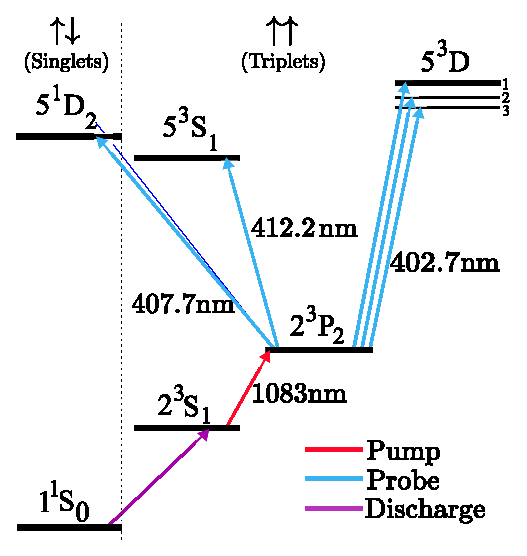
\includegraphics[width=\textwidth]{fig/Spectroscopy/level_diagram_tight_latex.eps}
% 	    \caption{A level diagram for the helium atom. The transitions measured in this work (blue), are driven by a tunable laser referred to in text as the 'probe'. The cooling transition (red) is referred to as 'pump' throughout the paper and populates the lower state of the target transitions.  The doubly forbidden $1\singlet S_0\rightarrow2\triplet  S_1$ transition is excited in a high voltage discharge cell. Transitions between the singlet and triplet manifolds (left and right of dotted line) are forbidden in the dipole approximation. The level splittings are not to scale.}
% 	    \label{fig:lvl_diag}
% 	\end{figure}

% \subsection{Detection scheme}\label{ssec:spec-detection}
% \begin{itemize}
% 	\item Setup - alignment
% 	\item Procedure
% 	\item Mechanism
% 	\item Calibrations
% 	\item Analysis
% \end{itemize}

% \subsubsection{Procedure}
% 	We use a micrometer translation mount on the final lens to align the beam on the Helium sample. We locate the transitions approximately by using the maximum available laser power at the predicted frequency, and then reducing the power and adjusting the frequency set point until the signal no longer saturates at the peak. We then scan the set point of the laser across the transition to obtain the transition signal.
% 	The beam was initially aligned by tuning the probe beam to the predicted value of the 53S1 transition and operating with the maximum available power. Although the uncertainy in wavemeter accuracy was larger than the transition linewidth, by operating well above the saturation intensity, the transition was broaded by tens of MHz and so the WM error was less significant. When scanning the beam pointing across the expected target region, approximate alignment was signaled by a dramatic loss of atom number. When the signal saturated, the power was lowered until the signal was just above the noise floor, and then scanning resumed. This process iterated a few times until the maximum attainable signal was below saturation - that is, when for fixed power one could not completely destroy the trap. Notice there are three kinds of saturation here: Atomic population saturation, detector saturation, and signal saturation when you run out of atoms. perhaps the term `dynamic range' would be more suited to the latter\ldots{} Something to think about.

% 	During the calibration shots, we also block the beam with a mirror mounted on an automatic translation mount. The profile and polarization of the beam are determined with lenses and waveplates prior to vacuum entry. The measurement sequence consists of measurement shots with each of the two magnetic field strengths followed by calibration shots, wherein the laser beam is blocked and switched off. We calibrate the wavemeter before each transition measurement. Analysis of the wavemeter stability suggests that calibration drift is not a significant source of error, as discussed in the supplementary materials.

% 	The method therefore consists of alternating measurement trials with control trials, wherein the laser beam is blocked before the fibre coupler with a flipper mirror. At the moment I use an interpolation, but I might want to try using a model-based estimate of the atom number. Either way, there is going to be some error in the number estimation. It's probably small. The difference between the interpolated, unperturbed atom number and the detected number in the measurement trials is affected by the quantum efficiency and the introduced uncertainty in atom number.

% 	The polarization of the light was fixed with the waveplates before the chamber. Can you tell handedness just by relative angle of waveplates? We hypothesized that the initial state of the atoms during the cooling phase was in the m=2 state, as the optics are configured to drive with a sigma+ beam during the in-trap cooling stage. I verified this by driving with plane-polarized light (in the atom frame - put some trap sim in to show where the field points), which is a linear combination of sigma+ and sigma- light. If there were atoms in initial states other than the m=2, then when driving to the 53S1 state, one would observe multiple peaks. Instead, only one peak was observed, which vanished when the probe beam was set to sigma+ light. (I think check the data).

% 	The measurements are taken at two different background field strengths. Therefore the detuning from cooling resonance is X and Y MHz in each stage, respectively. These values were calibrated independently by an RF spectroscopy technique. This allows empirical extrapolation to the field-free transition energy by correcting for the calculated Zeeman shift of the centre frequency of each measured line.


% % Peak intensity is ~ total power x 1e3 /m^2 for large beam
% \begin{table}
% \begin{tabular}{|c|c|c|c|c|}
% \hline
% Line & Beam waist (cm) & Beam power (mW) &  Peak intensity (W/m$^2$) & Exposure time (ms)\\
% \hline
% $5\triplet S_1$  & 4.1 &  2.73(1) & 3.1(2) & 100 \\
% $5\triplet D_1$  & 4.1 &  4.5(1) & 5.2(1) & 150\\
% $5\triplet D_2,3$& 4.1 &  8.6(1) & 9.9(1) & 250  \\
% $5\singlet D_2$  & 0.1 &  10(2) & 6.3E3 & 100 \\
% \end{tabular}
% \label{tab:spec-beamparams}
% \caption{Probe beam parameters}
% \end{table}
% \begin{table}
% \begin{tabular}{|c|c|c|c|c|}
% \hline
% Stage & Beam power & AOM detuning & Peak intensity & Transition detuning\\
% \hline
% \end{tabular}
% \label{tab:spec-pumpparams}
% \caption{Pump beam parameters}
% \end{table}

% \subsubsection{Data acquisition}
% 	\com{This probably goes in the Intro/BEC machine part}

% 	Following the laser interrogation, the remaining atoms are gradually outcoupled from the trap with a pulsed atom laser. At the beginning of each shot, the LabView control interface writes a line to the log file with the parameters \verb|timestamp, laser_setpt, shot_type| where \verb|shot_type| is either \verb|stage_1|, \verb|stage_2|, or \verb|calibration|. When importing the data into the processing scripts, the 

% 	 As the laser set point is fixed for sets of three shots (one per field setting), 


% \subsubsection{Mechanism of action}
% 	
% 	To drive the transitions from the 23P2 state to the states in the n=5 manifold, I use the probe beam to disturb the near-resonant optical molasses cooling stage of the experiment. This follows the MOT loading and precedes evaporative cooling, and operates with XYZ beam parameters for XXX ms, and then with ABC beam parameters for YYY ms. I calculate that during these stages, the excited-state population is ZZZ per cent, which are then susceptible to scattering photons from the probe beam.

% 	I used the evaporative cooling sequence as a transducer between scattering-induced heating of the cloud and the final condensed number. I will present a quantitative sketch of the mechanism below, but one can also take a heuristic understanding from the following argument:

% 	The evaporative cooling we use to achieve Bose-Einstein condensation has stringent tolerances on initial phase space density, which increases with number and at lower temperatures. Tuning a radio chirp to the spin-flip transition from a trapped to an untrapped state and sweeping down to lower energies, higher-energy atoms are removed, the cloud rethermalizes at a lower temperature, and the phase space density increases. Higher-energy atoms spend time further from the centre of a harmonic magnetic trap. So, scattering photons from the probe beam heat the cloud, leading widening the velocity distribution, which drives more of the atoms into resonance with the radio chirp. The final temperature is determined by the endpoint of the radio chirp. Resonance with the probe light manifests as a signal in a reduction of the final population of the condensate.

% 	As I said, an essential part of our BEC production is an optical cooling and spin-polarizing stage which precedes the loading of our magnetic trap. This ensures a nice large atom number and low temperature. This give us a nice big phase space density, a dimensionless number which compares the length scale of quantum interference, the de Broglie wavelength, with the interparticle spacing given by the particle density n.~So, disturbances to this initial condition by atom loss or heating will reduce the phase space density input to the evaporation stage. The Bose-Einstein condensation threshold occurs when the phase space density crosses about 2 - for comparison, atmosphere has a phase space density about one ten millionth of that. One can therefore think of the RF evaporation as a phase space amplifier in the following way:

% 	Evaporative cooling works by creating a resonance between trapped and untrapped magnetic states of atoms with a specific Zeeman splitting by exposing the cloud to radio frequency radiation. Energetic atoms travel up the magnetic field gradient, shown by the thickness of the purple lines, to the ellipsoidal shell defined by a fixed field strength at which the atoms resonate with the radio waves. The atoms are then transferred into free states and leave the trap, taking with an amount of energy greater than the ensemble average. This basically cuts out the upper tail of the Maxwell-Boltzmann distribution, driving down the atom number, but also the temperature once the cloud rethermalizes. If you get this right, you continuously increase the phase space density by making the cloud cooler and smaller, until you get to BEC. The endpoint of the RF chirp fixes an upper bound to the energy of the trapped atoms, and hence a temperature. Then the phase space density can be estimated by counting the number of atoms you have left. We measure this atom number using Helium's unique detectability - by applying broadband radio pulses to the trap we free about 0.5\% of the atoms at a time, creating a series of pulses of coherent matter waves, known as an atom laser. This resolves on our detector as a series of discrete particle detection events, which we sum up with an abacus. So by controlling our independent variable, the applied laser frequency, we have a gain mechanism that allows us to measure the dependent variable, which is the phase space density reduction by resonant scattering of photons from the probe beam.

% \subsubsection{Calibration measurements}

% 	After the probe is applied during the optical molasses cooling, we use a standard forced evaporative cooling procedure. At the end of the sequence the atoms are in the metastable $2^3S_1$ state which exhibits a 19.8eV ground state separation. This internal energy enables single-atom detection by a multi-channel plate and delay-line detector stack with an efficiency of 8 per cent\cite{Manning10} to determine the atom number loss. We use a pulsed atom laser \cite{Manning10,Henson18} to transfer atoms to the untrapped state and avoid detector saturation.


% 	A translation mount on the final lens gives us micrometer precision in the placement of the focal point on the beam, which we use to align the beam on the trap, threading a ten micron needle in the dark 20 micro-radian accuracy.


% 	\begin{table}
% 	\label{tab:aom_calibration}
% 	\begin{tabular}{|c|c|c|c|}
% 		\hline
% 		RF centre frequency & Calibrated field strength (G) & AOM frequency (MHz) & Detuning (MHz) \\
% 		\hline
% 		XXX & 18 & 138 & 0.5\\
% 		XXX & 11 & 133.6 & 2\\
% 		\hline
% 	\end{tabular}
% 	\end{table}
% 	AO offsets 138MHz and 133.6MHz ?
% 	cooling transition is split 25.55 MHz, and 16.002 in stage 2
% 	Therefore the beams are (ish) detuned 0.5 and 2MHz respectively

% \subsubsection{Analysis}
% 	In this section I describe the data processing method used for the peaks, using the $5\singlet D_2$ line as an example.

% \subsection{Findings}\label{ssec:spec-findings}

% \subsubsection{Results}

% 	\begin{figure*}
% 	  % \includegraphics[width=\textwidth]{fig/Spectroscopy/pub_lines_j1.eps}
% 	  \caption{Measured line profiles for the $\PStateManifold_2\rightarrow 5\triplet  S_1$ (left) and   $\PStateManifold_2\rightarrow 5\triplet  D_1$ (right) transitions, with Lorentzian fits. On the horizontal axis is the probe laser frequency $\nu$, relative to the theoretical prediction for the magnetic field-free splitting. The vertical axis is the response as measured by atom number loss relative to the calibration shots. Theoretical predictions (vertical bars) are Zeeman shifted from the zero-field value according to the field calibration, with uncertainty (horizontal bars) dominated by uncertainty in background field strength. Lines obtained by measuring against an 18G and 11G background field are shown in red and blue, respectively. }
% 	  \label{fig:simple_lines}
% 	\end{figure*}


% \subsection{Determination of transition energies}\label{ssec:spec-processing}


% \begin{figure}
% 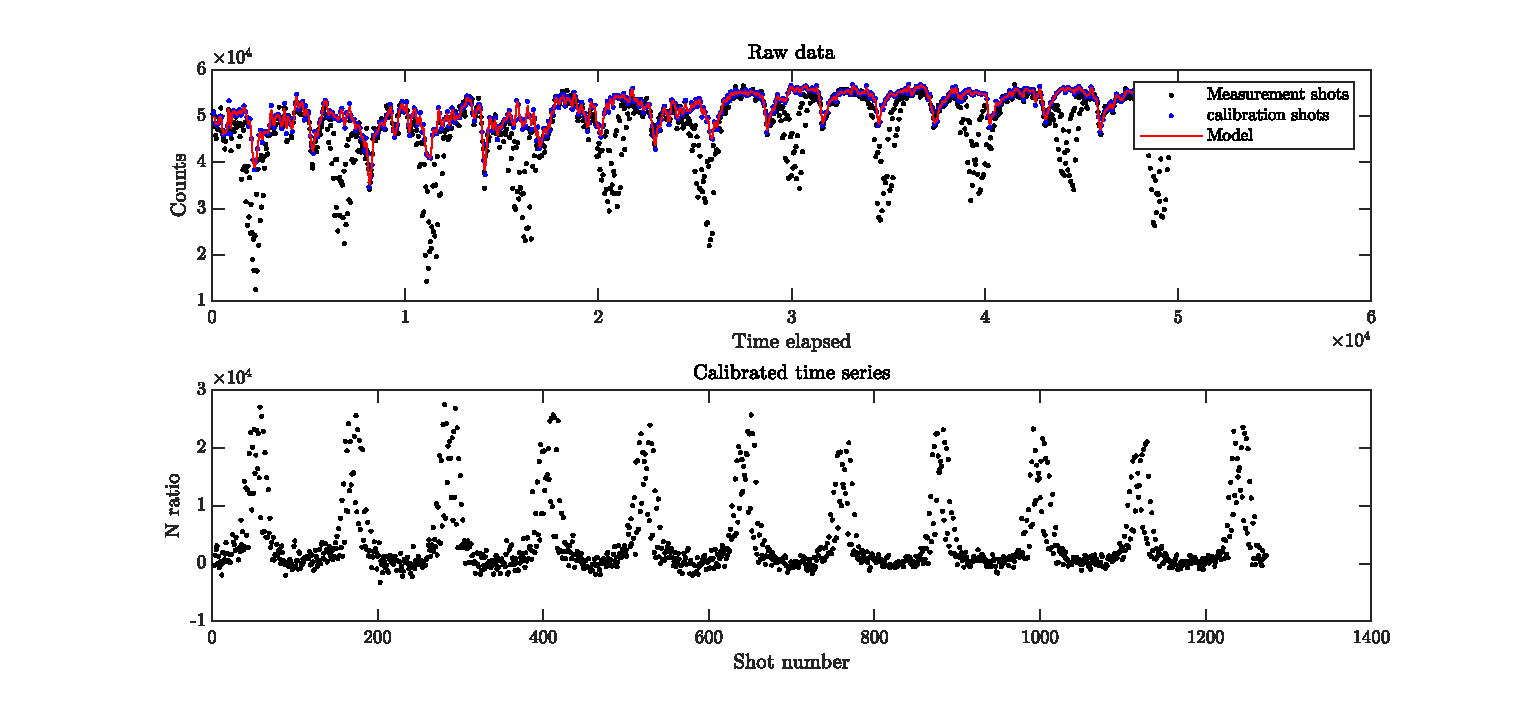
\includegraphics[width=\textwidth]{fig/spectroscopy/calib_model_51D2.eps}
% \label{}
% \caption{}
% \end{figure}

% \begin{figure}
% 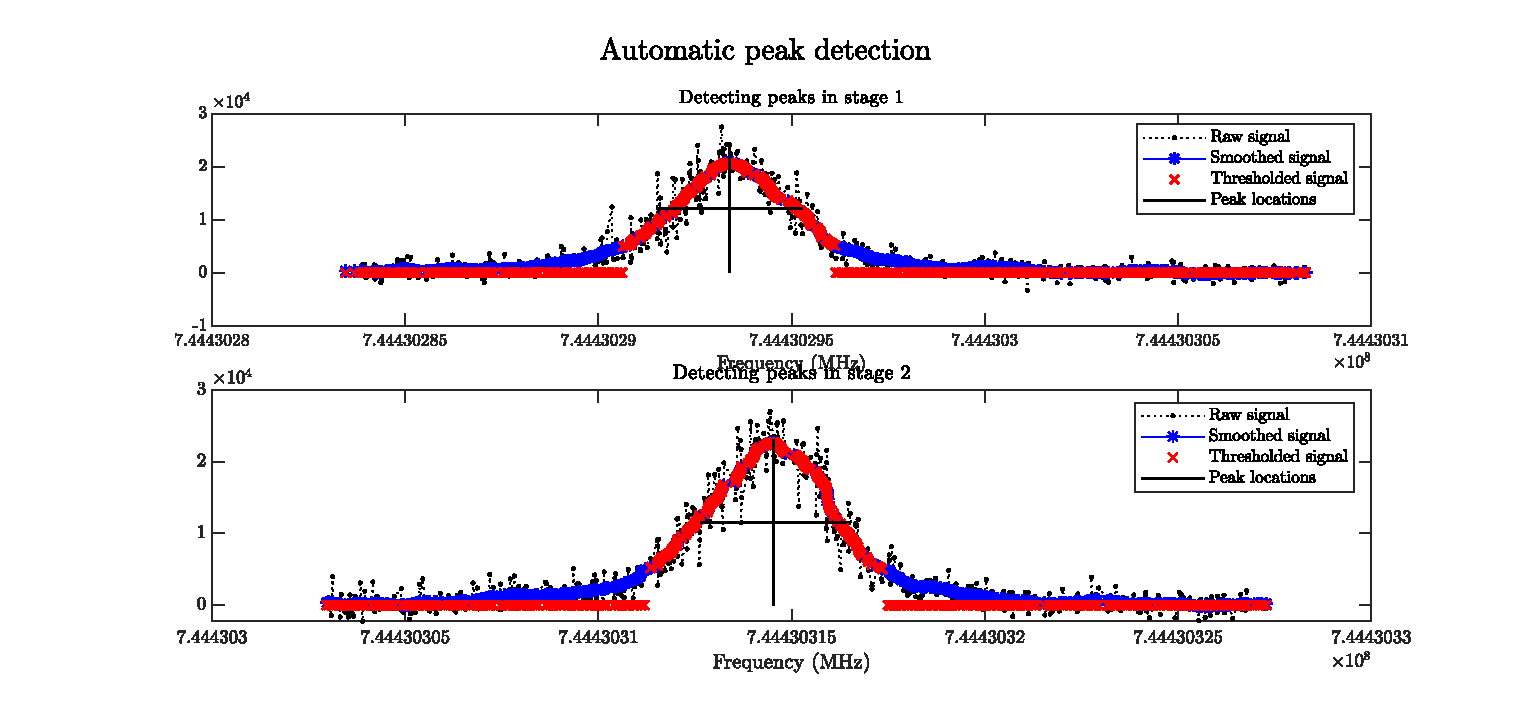
\includegraphics[width=\textwidth]{fig/spectroscopy/auto_peak_detect_51D2.eps}
% \label{}
% \caption{}
% \end{figure}

% \begin{figure}
% 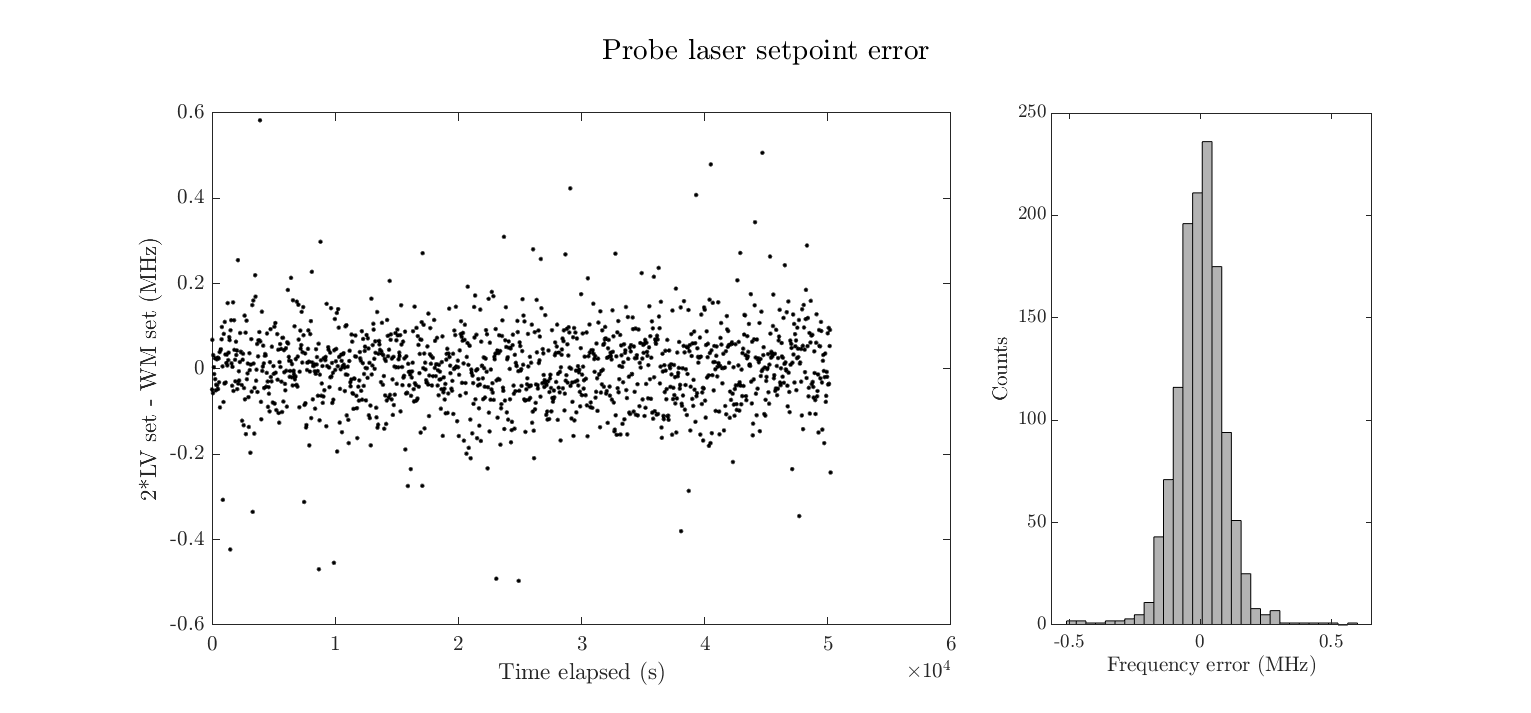
\includegraphics[width=\textwidth]{fig/spectroscopy/probe_set_err_51D2.eps}
% \label{}
% \caption{}
% \end{figure}

% \begin{figure}
% 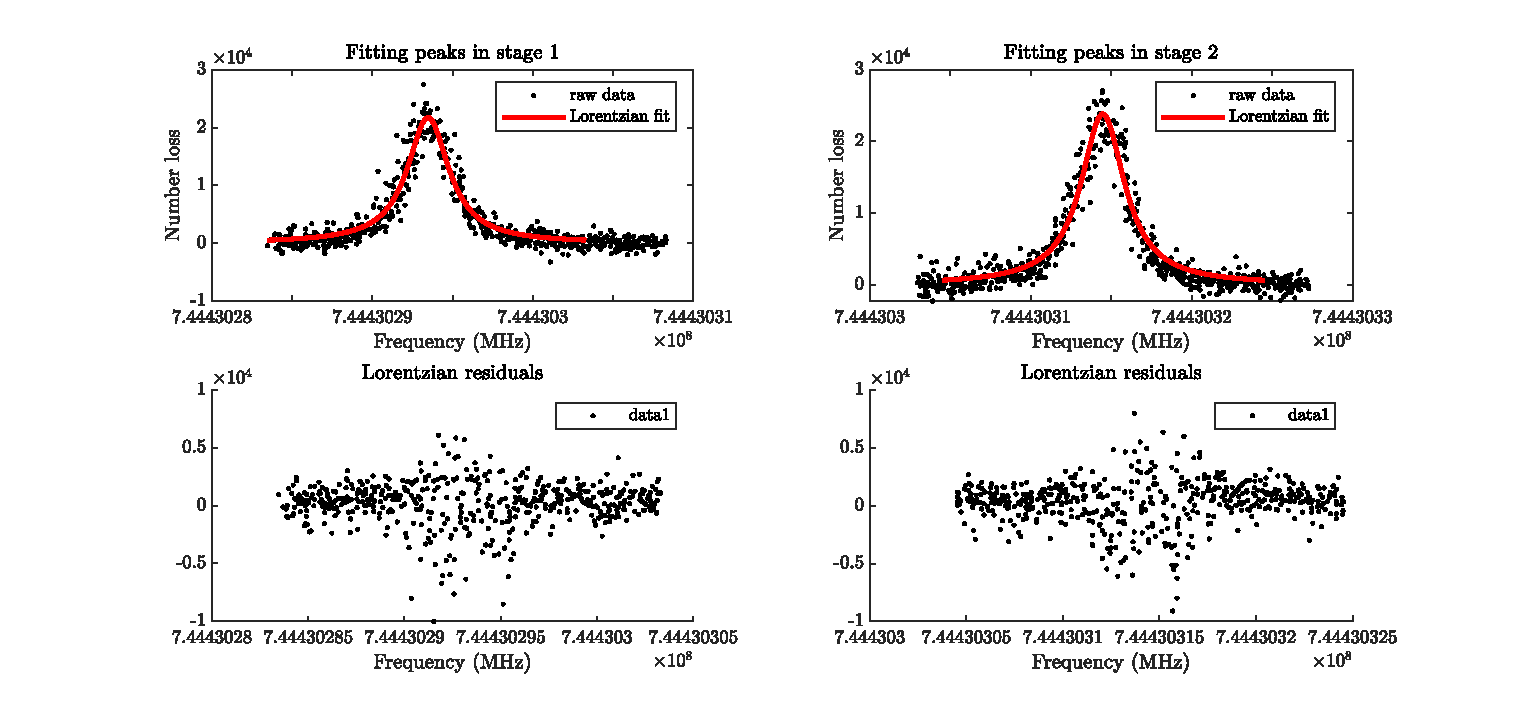
\includegraphics[width=\textwidth]{fig/spectroscopy/fitting_peaks_51D2.eps}
% \label{}
% \caption{}
% \end{figure}

% 	We empirically extrapolate to the field-free transition energy by correcting for the Zeeman shift in the observed lines. The exposure time and intensity varied among measurements to avoid saturation. 

% 	The table below displays the results of the measurements, including predicted linewidths. In the case of the 23S1-33S1, the measured Einstein A coefficient is also listed. These measurements are accurate to a few hundred parts per billion, and their accuracy is limited by the absolute accuracy of the wavemeter we used as a reference for the laser lock. Within the accuracy stated by the manufacturer, these results are consistent with the predictions of QED. Of the six lines measured, three have been resolved individually for the first time, and two have not been recorded elsewhere. The centre frequencies are obtained by fitting Lorentzian profiles to the atom loss spectra. Have a look at residuals; what are the expected broadening effects? What are the expected systematic errors? Error budget goes here also. 	

% 	Ah. The CG madness is only needed for the triplet D states. The singlet D and the triplet S have zero total angular momentum for the spin and orbital dof, respectively, so the basis is trivial and in these cases, we can use the linear extrapolation method with no worries. What about the 2 3P2? Oh - I missed a point, which is the presence of other nearby levels. For the singlet D, that's done, it's unique, as S=0. And for the triplet S, also, as L=0.  Not so for the 2 3P2. But they're several GHz away so that shouldn't be a problem at all. Well, then that's cleared up! Great. Now to write this nonsense up. Start concise in the paper, then we can expand it here. later.

% % A and Sum A from \cite{Drake07}
% % Triplet D: 8.3444E+02 1.3929E+07
% % 5 3S1 line 2.4738E+06 sum 9.2072E+06
% % 5 3DJ sum 1.6412E+07
% % 	Lines
% % 	J=1 3.2224E+05
% % 	J=2 2.8999E+06
% % 	J=3 1.1601E+07
% % 5 1D FROM 2 3P1 402.7151538 nm
% % the 2 3P J=1-2 interval is 2291.177 MHz from Zheng
% % line 8.3444E+02 sum 1.3929E+07
			
% % Two-peak results STAGE 1:

% % Widths: [4.30,5.73,3.03,3.14]
% % Two-peak results STAGE 2:
% % Centres: [744396208.29,744396204.67,744396182.37,744396224.64]
% % Widths: [4.94,4.26,3.91,3.60]

% % Centres_1: [744396195.49,744396191.21,744396160.46,744396223.01]
% % Centres_2: [744396208.29,744396204.67,744396182.37,744396224.64]

% % 3S_1 727303244.61
% % 3D_3 744396209.66
% % 3D_2 744396228.89
% % 3D_1 744396512.43
% % 1D_2 744430344.53

% \begin{table*}
% 	\begin{tabular}{|c||c c|c|c|c|c|}
%     \hline
%         $|e\rangle$ & $f_\textrm{meas,1}$ & $f_\textrm{meas,2}$ & $f_{\textrm{field-free}}$   & $\Delta_\mathrm{theory}$ & $\textrm{FWHM}_\textrm{obs.}$ & $\textrm{FWHM}_\textrm{pred.}$  \\
%     \hline\hline
%         $5^3\mathrm{S}_1$    & 727,303,223.89 &				& 727,303,249(5)   &   4.4    &  3.12(40)& 9.21\\ % A = 
%                              & 727,303,234.04 &				&		& 			 & 		&	\\
%         \hline
%         $5^3\mathrm{D}_1$    & 744,396,453.41 &				& 744,396,496(21) & -16  &  5.79(62) & 16.4\\
%                              & 744,396,477.82 &				& 		& 			 & 	&	\\
%         \hline
%         $5^3\mathrm{D}_2$    &  744,396,191.21 & 744,396,223.01  & 744,396,217(22)  &  -12 & 4.18(50)  &16.4\\
%                              &  744,396,204.67 & 744,396,224.64 & 		& 			 &  &	\\
%         \hline
%         $5^3\mathrm{D}_3$    & 744,396,160.46 & 744,396,195.49 & 744,396,201(21) &  -8.7 & 4.04(12)   &16.4\\
%             			     & 744,396,182.37 & 744,396,208.29  & 		& 			 & 		&\\
%         \hline
%         $5^1\mathrm{D}_2$    & 744,430,295.37 &				& 744,430,347(21) &  2.5  & 3.21(13)  & 13.9\\
%                              & 744,430,316.37 &				& 		& 			 & 		& \\
%         \hline
% \end{tabular}
% \label{tab:spec-results}
% \caption{Summary of results (all in MHz) For each transition. The measured frequencies are obtained in an ambient magnetic field of strength 18G (top row) and 11G (bottom row). After correcting for the AOM and vapor cell shifts we extract the centre frequencies $f_{meas}$ from Lorentzian fits with statistical error at the $~ 10\textrm{kHz}$ level. For the $5\triplet D_2$ and $5\triplet D_3$ states, each line shows the pair of transitions corresponding to the magnetic quantum number of the upper state $m_u=1$ and $m_u=2$, respectively. After correcting for Zeeman shifts, the field-free energies $f_{\textrm{field-free}}$ are obtained, and shown with statistical error in parentheses. We show the difference $\Delta_\mathrm{theory}$ between our measurements theoretical predictions \cite{Drake07}. Observed line widths are the mean full width at half maximum $\textrm{FWHM}_\textrm{obs.}$ of a Lorentzian fit to each line, with theoretical predictions $\textrm{FWHM}_\textrm{pred.}$ from \cite{Drake07}.}
% \end{table*}
% 	\begin{figure}
% 	  % \includegraphics[width=\textwidth]{fig/Spectroscopy/pub_lines_5D1.eps}
% 	  \caption{Line profile for the spin-forbidden $\PStateManifold_2\rightarrow 5\singlet D_2$ transition, presented similarly to figure \ref{fig:simple_lines}.}
% 	  \label{fig:3D_1_line}
% 	\end{figure}


% 	\begin{figure}
% 	  % \includegraphics[width=\textwidth]{fig/Spectroscopy/pub_lines_5D2_3.eps}
% 	  \caption{Line profiles for the $\PStateManifold_2\rightarrow 5\triplet  D_{2}$ and $\PStateManifold_2\rightarrow 5\triplet  D_{3}$ transitions, driven by a mixure of $\sigma^-$ and $\pi$- polarized light and presented similarly to figure \ref{fig:simple_lines} and \ref{fig:3D_1_line}. The large central peak is the overlap of two peaks, the transitions to the XXX and YYY lines, which are nearly degenerate for the entire operational range of our background magnetic field.}
% 	  \label{fig:3D_23_lines}
% 	\end{figure}
% 	Figure 2 shows the spectra measured using this technique. Table I summarizes the results of our measurements. An account of our error budget is given in the supplementary materials, and summarized in Table II.  While we are able to resolve the $5\triplet  D_1$ peak, the $5\triplet  D_2$ and $5\triplet  D_3$ resonance are sufficiently close together to cause significant quantum interference effects \cite{Marsman15}, and require special treatment to obtain the zero-field values. 

% \subsubsection{Error budget}

% 	The statistical error in the centre frequency of our Lorentzian fits is less than a MHz, fixing these transitions to some parts per billion, with MHz differences from theory. The last measurement of the 2\textsuperscript{3P-5}3D gap could not resolve the fine structure splitting, about 300MHz, but we resolve them with excellent visibility. To give credit where credit is due, the last measurement of these transitions used a discharge cell submerged in liquid nitrogen, passed through a window to an in-vacuum diffraction grating and illuminating a phosphor screen with lines whose splitting was measured with a ruler against a Mercury reference. Still, they were wrong.

% 	But, our ultimate accuracy is limited by the wavemeter to 20MHz in the worst case, or 4MHz when close enough to the calibration line. Unfortunately, we don't have the precision required to compete with the state of the art, but had we a frequency comb reference then we'd be in the game for tests of fundamental physics. Still, we correct the previous values by thirteen gigahertz, update four values in the NIST database, and add a new line to boot. We conclude that within our experimental uncertainty, QED is correct.

% 	The AC Stark effect from the probe beam varies between the measurements, but in all cases is calculated to be less than 1MHz, in agreement with an empirical determination described in the supplementary materials. The recoil shift is ambiguous in sign because of the counterpropagating pump beams, but the shift is at least an order of magnitude less than the absorption linewidth.

% 	\begin{table}[h]
% 	\begin{tabular}{|c|c|c|}
% 	    \hline
% 	        Source & Shift (MHz) & Unc. (MHz)  \\
% 	    \hline\hline
% 	        AC Stark (Pump) & $<$0.1 & -\\
% 	        AC Stark (Probe) & $<$1 & -\\
% 	        DC Stark & $<$0.1 & - \\
% 	        Mean field & $<$0.1 & -\\
% 	        Recoil & $\pm0.218$ & 1 \\ % assume angle accurate to 1deg
% 	        Wavemeter & 0 & Variable \\
% 	        Doppler & XX & YY \\
% 	        Pump lock & N/A & 0.3 \\
% 	        Probe lock & -190MHz & 0.1\\
% 	        Cs cell & -1.9 & 4 \\
% 	    \hline
% 	        Total & -1.9&4.1+WM\\
% 	    \hline
% 	\end{tabular}
% 	\caption{Error budget for the measured lines. }
% 	\end{table}

% \subsubsection{Discussion}

% 	We improve on previous measurements with an order of magnitude greater precision and report the first observation of the spin-forbidden $2\triplet  P_2\rightarrow5\singlet D_2$ transition in Helium. Our measurements constrain the $5\triplet  D$ and $5\singlet D$ ionization energies of $^4$He to 150 parts per billion, and the $5\triplet  S$ $5^3S$ to 28 parts per billion. The theoretical transition energies agree with the observed values within experimental error.

% 	We performed multilevel laser absorption spectroscopy of excited states with ultracold atoms in hard vacuum. Our measurements agree with current predictions within our error budget. A $93\sigma$ difference between Martin's measurement\cite{Martin60} and predictions \cite{Morton06} of the $\PStateManifold_2 \rightarrow \UpperS$ and $\PStateManifold_2 \rightarrow \UpperStateManifold$ intervals are resolved by this work.  Our measurements constrain the $5^3D$ and $5^1D$ ionization energies of 4He to 150 parts per billion, and the $5^3S$ to 28 parts per billion. This work provides four contributions to the NIST database of atomic spectral lines. 

% 	In Martin's original paper, he only quotes measurements from $\PStateManifold_2-5D$, indicating that his equipment did not have the resolving power to distinguish the fine structure of the $5D$ state. Martin's measurements were made using a nitrogen-cooled Helium discharge lamp fed through an in-vacuum prism onto photographic plates where line separations were measured with a ruler. 

% 	The apparatus used for this experiment is presently being upgraded to operate with $^3$He - $^4$He mixtures. This technique could be employed, along with an improved frequency reference such as a clock-stabilized frequency comb, to constrain the charge radius difference for comparison with other transitions.



% \section{Detection of the forbidden $2\triplet  S_1\rightarrow3\triplet  S_1$ transition}\label{sec:forbidden}

% 	After our measurement of the 2P-5L transitions, our eyes turned to the 427nm transition. To our knowledge, nobody had measured it. We found that we required ten orders of magnitude greater sensitivity in order to detect this transition - a few mW over a few ms wasn't going to cut it. After discussion we decided that the most promising method might be to look for heating or loss by directly illuminating a BEC - having found previously that weak trap lifetimes can in fact be several minutes. However, before we embarked on the measurement, I performed some simple calculations to estimate the order of magnitude of the best signal-to-noise ratio we could expect.

% 	We determined that this SNR would be sufficient to warrant making an attempt at the measurement.

% 	RECOUNT CALCULATION * 3 level measurement * Clebsch-gordan coefficients
% 	and net transition rates * Collection efficiency monte carlo

% 	For this measurement, the data processing methods were the similar to the 5L transitions - a drift model was created to predict the undisturbed atom number in a given shot, based on atom number measurements from the calibration shots. Wait - did the outcoupled fraction get used, counting the number dropped versus the number left in the trap? Were these things tried? Talk to Kieran.

% 	This method allows for the extraction of the line centre and width, which determines the state lifetime. However, the state lifetime is dominated by a fast decay to the 3P state, the oscillator strength of which is many orders of magnitude larger. The oscillator strength - which is proportional to the Einstein A coefficient - of the transition can be obtained by another method, described in the next section.

% 	We develop a second method to determine the Einstein A coefficient of the specific forbidden transition. We perform time-dependent thermometry of the a thermal cloud (above the critical temperature) while alternating shots with and without the probe beam blocked. During these sequences, we use RF pulses as per standard procedure (although in this case the term `laser' is especially misleading as the source is incoherent) and fit a Gaussian profile to each pulse. During the 25 second hold time, the cloud heats at a rate of X K/sec.~This is possibly due to: Penning ionization, magnetic field noise, background collisions, majorana leaks? How does it depend on number? Anyway. With the probe beam applied, the calculated scattering rate of up to Y Hz corresponds to a peak additional heating rate of Y J/sec.

% 	We fit the time evolution of the temperature of the thermal cloud with a linear model and obtain the change in heating rate with respect to the probe-free shots. We can then back-calculate via the specific heat of a harmonically trapped Bose gas to determine the energy transfer rate (which should just be proportional I think, when above the critical temperature?), hence the photon scattering rate. And so lo and behold we can determine the A coefficient, and look, it's really weak! What a great job we did. I wonder whether Kieran's method is a bit sketch because does heassume a certain density distribution??

% 	Power \& curvature measurements - what actually drives Quadrupole
% 	transitions?
% \subsection{Proof-of-feasibility calculation}\label{ssec:forbidden-feasibility}
% \subsection{Two detection methods}\label{ssec:forbidden-methods}
% \subsection{Findings}\label{ssec:forbidden-findings}
% \subsubsection{Error budget}
% \subsubsection{Results}

% 	Isotope shifts \& better reference 
% 	Different target transitions?

% https://physics.stackexchange.com/questions/430532/why-are-there-no-transitions-between-orthohelium-and-parahelium





% \chapter*{A: Forbidden}
% \chapter*{A: Tuneout}

% % % % \part*{Inflection point}

% \part{Many-body physics in ultracold gases}
% % \hypertarget{many-body-physics}{%
% \section{Many-body physics}\label{many-body-physics}}
% \chapter*{Interplay, emergence, complexity}
% \addcontentsline{toc}{chapter}{Interplay, emergence, complexity}
% \section*{There's always a bigger Hilbert space}%stat phys, Thermalization, coherence, quantum matter, state engineering
% \addcontentsline{toc}{section}{There's always a bigger Hilbert space}
\subsection*{It to bit}% QMI/condmat, QML, church-turing, Physics as a branch of computer science, process theories?
\subsection*{Over the horizon}% Exotic matter, quantum simulation, is this more like string theory or thermodynamics? 

\begin{adjustwidth}{3cm}{0cm}
\begin{flushright}
\emph{``From the Tao comes one,\\
from one comes two,\\
from two comes three, and\\
from three comes all things."}\\
 - Lao Tzu\footnote{Tao Te Ching, circa 4th-6th century BCE}
\end{flushright}
\end{adjustwidth}
    


	% [Many body phys] I bloch, J Dalibard, W Zwerger many-body physics with ultracold gases, rev mod phys 80, 2008
	% [Many body phys/scattering] C Chin et al, feschbach resoannces in ultracold gases, rev mod phys 82, 2010

	What actually happens when you add more particles? What do we mean things get more complex - what resources are there more of in the state, and what does it take more of to simulate etc
		% https://journals.aps.org/rmp/abstract/10.1103/RevModPhys.82.1225 feshbach resonance review
Oh look, this might be handy https://arxiv.org/pdf/1711.04105.pdf
	Ingo Peschel shows that one can determine reduced density matrices from correlation functions of lattice systems \cite{Peschel03} %https://iopscience.iop.org/article/10.1088/0305-4470/36/14/101/fulltext/ 	(reduced) density matrices of solvable models have the form $\exp(-H)$, where $H$ is a solvable operator confined to the chosen subsystem (this is in the context of dmrg). You just integrate/trace out the degrees of freedom outside the subsystem.


	% Kibble-Zurek mechanism and criticality?
	% Pichler et al 2010 nonequlibrium dynamcics of bosonic atoms in optical lattices: Decoherence of many-body states dues to spontaneous emissions, phys rev a, atomic molecular and optical phscs 82
	% Sachdev QPT book
	% RSP [97,96] classical phase transitions are accompanied by non-analytic free energy (deriv. of partition fn?) and micro fluctuations (thermal) actually cause the transition 
	% RSP in contrast to Quantum phase transitions occur when tuning g in H = H0 + g H1, where [H0,H1]!=0 - and can occur at T=0, usuall refer to ground state transitions, dominant character of state changes due to eg avoided crossing? 
Section introduction\\
Statistical physics Phase transitions\\
Thermal, quantum, dynamical, computable, semantic Emergent complexity

The third section of this thesis transitions from the study of atomic
structure to the emergent dynamics of interacting systems. In teh old
essay `More is different', there is an argument that when you put a lot
of thigns together they start acting in genuinely novel ways. A single
water molecule is not wet - nor does it mean anything to say it is any
given phase, or that is has a temperature. (this is of course
problematic because it ascribes a specific state but the idea's there I
guess). So ya. One of the watershed(?) moments in the history of physics
was the \emph{derivation} of thermodynamics from statistical mechancics
- the assumption of a set of postulates about the microscopic nature of
the world that led through the law of large numbers to a new
understanding of empirical laws of the past; this gave a framework to
understand and extend thermo, and it was a triumph to provide systematic
ways to determine macro physics from teh nature of interactions. What
was more profouond was the discovery of universality classes - that at
phase boundaries there were unifying properties across disparate
systems, things that tied together quite general phenomena in terms of
these scaling relationships. This is kind of garbled. But yeah, look, we
have agaaghagha this is just insane rambling - I wonder if I can push to
10k words in the process of smooshing out all this. Not an entirely
honest drive if I'm honest but w/e the thing is I'm here and I'm writing
even if it's completely useless and will get trashed. This is a start,
even if it's bogus and hard. Anyhow back to progress. So ya -
statistical mechnics also provided an actual understanding of
temperature as a sublime phenomenon in all the emergent phenomenon -
that really, at the end of the day, thermal equlibrium and the
`spontaneous' processes we see in nature are just outcomes of,
basically, the law of large numbers. Phase transitions have been noted
in all kinds of places now; the BEC transitiion is a classical phase
transition. The idea is that an \emph{order parameter} changes value
from zero - representing a kind of disorganization - to something
nonzero, representing an emergent order. These come in different
flavours and in different systems but tied together by their scaling
laws - universality classes. Something really beautifully profound
there. And of course, pepole have tried to take the numinous idea of the
phase transition, of the \emph{qualitative} change in the emergent
properties of otherwise unchanged constituents, just by fiddling how
they relate to each other - and staple it to all kinds of things. People
talk of phase transitions in general network theory, presumably in
social dynamics, and more recently even in the study of grammars,
arguing that meaningful language corresponds to a marked phase
transition in lexical trees. But turning back from flights of fancy -
thermodynamics unified these ideas (in the earlier days) with the idea
of \emph{Free energy} which has since run rampant. But the idea is that
- well, if you have tunable parameters, then are there different
solutions to some equation? How do you wind up with these multiple
free-energy landscapes from a microscopic basis? Or do you need to
staple models toether? Idk, this would have been a great topics for a
PhD, hey?

Regardless. The idea is that we should probably add more signposts to
this meandering mess. I want to lead from classical phase transitions to
order parameters - using BEC as an example, identify its universality
class, no need to list off a ton or ramble about them too much. Then say
hey, once you're in the ground state, you have different kinds of phase
transitions. Quantum phase transitions, which aren't driven thermally or
by statistical laws but by the structure of the gruond state, and they
were first observed in an optical lattice. Free energy comes up as
should correlations, I think, as they both come hand in hand with order
etc.


Information In which the prospects of a quantum simulator are outlined. Beginning
with the discussion of a qubit and then the purity of states, the quantum analog
algorithms will be described. The necessity of state purity i.e. low entropy should
be discussed, and the question of realizing a high-purity quantum register should be
suggestively posed.
 Turing machines
 qubits
 Bloch sphere and evolution
 Purity
 Density matrix and the trace operator
 entanglement
 decomposition (partial traces, Schmidt product)
 second quantization
 coherence
 entropy
 renormalization
 thermodynamics
 thermalization
Matter In which the realization of the quantum analog algorithm is fixed in the form of
an optical lattice. The theory of atom-light interactions should be presented, and
the content of any field theories describing the composite system. Where possible,
connections should be drawn to the preceding chapter, and also to experimental
considerations which will be treated in the next chapter.
 Atomic structure
 metastable helium
 light and two-level atoms (qubits)
 Scattering and the radiative force
 Dipole force
 Sublevels
 Zeeman effect
vii
viii
 Angular momentum, polarization, and spin
 Composite systems
 Matter fields
 Correlation functions
 Strongly correlated systems
 Effective field theories: Bogoliubov and Bose-Hubbard
 Information revisited
 Comments on thermodynamics of cold atom ensembles
{ Breakdown of the equipartition theorem and kinetic temperature
{ Efficiency of atomic refrigeration
{ Quantum propagators, thermodynamics, and imaginary time
 Comments on classical, semiclassical, and quantum models
{ Breakdown of assumptions of continuity
{ Classical and quantum dipoles
{
Neural Networks In which any work done on representation of the quantum system is
decribed, along with precursors to any calculations done with these methods. In
this section, connections should be drawn between deep learning/state representation/
tensor networks/renormalization/state production/physical computation. It's
the dream. It's where it all comes together, but also the chapter that will be the
hardest or least likely to produce.
 Matrix product states
 MERA
 quantum circuit model
 RBM, DBM, and representations
 Deep learning and renormalization
 algorithms: tradeoffs and advantages
 categorical formulation
 Equivalence of circuits, ANN states and quantum states
 Church-Turing in the age of QNN and ANNQS
 Curry-Howard and state preparation

 Introduction
Perspective
 Ultra low temperature atomic physics
 Scenic Tour: Computing, quantum challenges
 Quantum simulators
 Optical lattice
Process of physical science
 Game of regularity: New understanding for free
 Triumph of reason: expressivity from compression
 Engineering requires correspondence: unpacking
 Quantifying computational effort
Computing and physics
Machine-assisted Phenomenology
 Convenient to outsource calculations
 How do you accurately predict the future?
 How much does it cost to predict the future?
Cost of computation
 Resolution/memory/time tradeoff
 RSA relies on problems being hard
Going Quantum
Simplifying matters
 Renormalization retains information while reducing dimensions
 Strongly correlated systems: modest many body systems impossible on
classical computers
1
Going Quantum
 One resolution to exponential memory demands
 universal quantum computer models ANY QUANTUM PROCESS
Quantum supremacy
Where's my QC?
 decoherence: arbitrary phase noise
 quantum errors are continuous: harder than bit 
ips
 Error correction threshold unreached, adds overhead
 Universal quantum computing and effciency
 Google's 50 qubits
Comments on complexity
 "Best possible classical algorithm"
 Sorry there's no clear cut definitions
 What is different about quantum computers? Open question.
Feynman's Big Idea
 System replication
 Run experiments on the model system and translate them back
 Move the goal posts: Solve (simulate) specific problems
 hope the simulation is "more effcient" than anything else: difference be-
tween impossble and achievable
Optical Lattices
Lattice overview
 Atom-light interactions (lasers) provide control
 Versatile: HEP, condensed matter, quantum information
 Approaching strongly-correlated regime
2
Quantum Phase Transitions
 Potential depth determines importance of interactions
 Eventually tunnelling suppressed by interactions: MI
 partial localization leads to interference
 MI phase incoherent
Simulations
 Also: Artificial graphene, non-thermal states, negative temperatures
 Role of entanglement in thermalization
 In the pursuit of effective representations of physical systems we have built
devices that create small-scale controllable simulations of the quantum
fabric of the universe. Cool, huh?
 Fundamental quantum mechanics necessary for quantum engineering
Quantum supremacy?
Research at ANU
ANU lattice
 Dipole force creates lattice
 Dipole barely overcomes gravity: Atoms must be ultracold to remain
trapped
 laser cooling: 3 nobel. BEC: 3 nobel.
 condensation: Macroscopic wavefunction
Conclusion
 High-resolution quantum dynamics in artifical crystal
 Such systems hard to simulate with existing computers
 No universal quantum computer, so specialized simulator
 Other groups: Have data out of reach of modern computing!
 Not known whether this is 'supreme'
 Analog simulators probably bridge the gap between classical sims and
universal quantum



    https://journals.aps.org/prl/abstract/10.1103/PhysRevLett.124.073401 



% \chapter{Quantum depletion of a harmonically trapped Bose gas}
% % \hypertarget{quantum-depletion}{%
% \section{Quantum depletion}\label{quantum-depletion}}
\chapter{Quantum depletion of a harmonically trapped Bose gas}
\label{chap:QD}

\begin{adjustwidth}{3cm}{0cm}
\begin{flushright}
\emph{``Do not be content with the answer that is almost right; seek one that is exactly right...
	The Way is a precise Art.
	Do not walk to the truth, but dance."} - Eliezer Yudkowsky\footnote{\url{http://yudkowsky.net/rational/virtues/}}
\end{flushright}
\end{adjustwidth}


\section{Introduction} 
	One of Bogoliubov's seminal cotributions was to formalize the role of Bose-Einstein condensation in the physics of superfluidity \cite{Bogolubov47}.
	the mechanism underlying superfluid formation is the Bose-Einstein condensation of collective excitations.
	
	By transforming from the picture of a homogeneous system of interacting bosons to that of a free Bose gas of non-interacting quasiparticles, Bogoliubov showed that the macroscopically-occupied quasiparticle ground state corresponds to the superfluid part of the Landau two-fluid model.
	The population of excited quasiparticle modes then makes up the normal component of the fluid.
	
	This foundational theory is of broad relevance because the BEC and BCS regimes of superconductivity are characterized by superfluids of molecular dimers and of Cooper pairs, respectively.
	  

	In a bose gas, the collective excitations are constituted by oppositely-moving particles \cite{Vogels02}.
	
	Repulsive interactions between constituent particles lead to a zero-point population of quasiparticle modes, known as the quantum depletion, which persists even at zero temperature.
	
	The quantum depletion presents as an occupation of single particle modes with large momentum $p$ that decays like $p^{-4}$.
	In liquid helium, the depleted fraction is large (of order 90\% of the fluid) due to the strong interparticle interactions, but is generally very small in weakly-interacting dilute gases.
	Bogoliubov's theory makes accurate predictions of the total depleted population in ultracold atomic Bose-Einstein condensates (BECs) \cite{xu06,lopes17_depletion} and exciton-polariton condensates in solid substrates \cite{pieczarka20}.
	Therefore, detailed study of the quantum-depleted tails of the momentum distribution in ultracold gases is an attractive test for the Bogoliubov theory.

	This has been challenging to date because the tails are usually beneath the noise floor of optical imaging techniques, wherein the momentum spectrum is mapped onto the far-field density distibution following ballistic expansion.
	The use of Feshbach resonances to enhance the quantum depletion in strongly-interacting Bose gases has garnered recent attention \cite{Makotyn14,Fletcher17,Eigen18}.
	Measurements of the momentum distribution in these settings \cite{Makotyn14,Eigen18} found tails that deviate from the power-law behaviour, and a handful of theories have emerged \cite{Kira15_coherent,Colussi20,Smith14} in effort to understand this finding.
	
	While the particulars are still under debate, the general picture is that three-body interactions play important roles in the dynamical response of the gas to a switch to a large scattering length.
	In contrast, another meaurement in the a weakly interacting regime reported unexpectedly large momentum tails in the far-field density of a helium BEC released from a harmonic optical trap \cite{Chang16}.
	
	This is particularly surprising because conventional wisdom argues that the density decreases adiabatically during expansion, justifying treatment with a hydrodynamic approximation wherein the tails are predicted to vanish \cite{Qu16}.
	

	These observations are also in conflict with quantitative predictions of the tail shape drawn from the theory of contact interactions developed by Tan \cite{Tan08_energetics,Tan08_momentum,Tan08_virial}.
	The thermodynamic quantity called the \emph{contact} characterizes how s-wave contact interactions modify the short-range pair correlation function.
	
	The dual manifestation of this modification is that the contact determines the amplitude of the power-law decay of the momentum density in terms of the gas density and s-wave scattering length, which fully determine collisional dynamics in ultracold dilute gases.
	
	Two central properties of the contact, known as the adiabatic sweep theorem and generalized virial theorem \cite{Tan08_momentum,Tan08_virial}, have been verified via radio spectroscopy \cite{Baym07,Punk07,Braaten10} of degenerate Bose \cite{Wild12} and Fermi gases \cite{Stewart10,sagi12}.
	
	While the Bogoliubov prescription breaks down in strongly-correlated systems \cite{Lopes17_quasiparticle}, Tan’s theory applies for arbitrary spin mixtures at any density, temperature, and geometry, and so both theories are expected to agree in the weakly interacting regime.

	Thus, it is surprising that the prior work reported such strong tails as this apparently contravenes both the Tan and Bogoliubov theories in the weakly-interacting regime where both have otherwise been demonstrated to be accurate.
	One possible implication of this finding would be that some feature of harmonically trapped helium condensates violate the minimal assumptions of both theories, which would warrant further study.
	On the other hand, far-field measurements in general might not provide a straightforward means of examining the quantum depletion even in weakly interacting gases.
	As far-field measurements play a central role in study of ultracold gases, it is important to verify the anomaly and understand its origin in order to glean further insight.

	To this end, we revisit the measurement of the momentum distribution of a helium condensate expanding from a harmonic trap.
	
	We conducted experiments using a different apparatus, covering a range of densities twice as large as the prior work and using a magnetic trap in place of an optical dipole trap which ensures perfect spin-polarization of the condensate.
	
	We observe tails in the large-momentum part of the condensate wavefunction whose population is controllable in a manner consistent with the Tan and Bogoliubov theories.
	However, we show that not much can be said with certainty about the $p^{-4}$ decay due to inherent difficulties one faces when analysing power-law distributions in general.
	
	We describe, in detail, the limitations of inference of power-law parameters from empirical data with particlar emphasis on the relation between our findings and the results reported in \cite{Chang16}.
	
	Our measurements are complemented by simulations of the time-dependence of the momentum distribution using a stochastic Time-Adaptive Bogoliubov (STAB) method in the positive-P framework \cite{Deuar11,Kheruntsyan12}.
	
	These show that the non-adiabatic release of the trap is responsible for survival of the depletion, and that the depleted particles acquire additional kinetic energy from the mean-field energy of the condensate during the subsequent adiabatic expansion.
	
	These factors result in an amplification of the momentum tails relative to the in situ values, and are not captured in the hydrodynamic approximation.
	
	
	Finally, we discuss the concordance between our theoretical and experimental investigations in support of the visibility of the quantum depletion in the far-field and suggest productive means for future investigation.
	
\section{Background} 
	The Hamiltonian of a homogeneous system of interacting bosons can be written in terms of plane-wave field operators $\hat{a_\kvec}$, labeled by the wavevector $\kvec=\textbf{p}/\hbar$, as
	\begin{equation}
		\hat{H} = \sum_{\kvec} \frac{\hbar^2k^2}{2m}\hat{a}_{\kvec}^\dagger \hat{a}_\kvec + \frac{g n}{2}\sum_{\kvec,\kvec',{\bf l}}\hat{a}_{\kvec+{\bf l}}^\dagger\hat{a}_{\kvec'-{\bf l}}^\dagger \hat{a}_{\kvec'}\hat{a}_{\kvec},
	\end{equation}
	in terms of the particle density $n$ and the effective interaction strength $g=4\pi\hbar^2a^2/m$, where $a$ is the s-wave scattering length and $m$ is the atomic mass \cite{PitaevskiiStringari,PethickSmith}.
   
    This Hamiltonian can be diagonalized by the Bogoliubov transformation to a free Bose gas of collective excitations through the operator transformation $\hat{b}_{\kvec}^\dagger = u_k \hat{a}_\kvec^\dagger + v_k \hat{a}_{-\kvec}$ \cite{Bogolubov47,PethickSmith}, where the $u_k$ and $v_k$ coefficients are given by
	\begin{align}
		u_{k}^2 &= \frac{1}{2}\left(\frac{\hbar^2k^2/2m + gn}{\epsilon(k)} + 1\right)~\textrm{and}\\
		v_{k}^2 &= \frac{1}{2}\left(\frac{\hbar^2k^2/2m + gn}{\epsilon(k)} - 1\right),\\
	\end{align}
	and where the denominator is the quasiparticle dispersion
	\begin{equation}
		\epsilon(k) = \sqrt{\left(\frac{\hbar^2k^2}{2m}\right)^2 + gn\frac{ \hbar^2k^2}{m}}.
	\end{equation}
	In the non-interacting ($a\rightarrow0$) limit, $u_k=1$ and $v_k=0$, so the transformation reduces to the identity and the dispersion is that of free particles.
	
	In general, the single-particle momentum density can be found using the inverse transformation and is given by
	 \begin{align}
	 \rho(\kvec) &= \langle\hat{a}_\kvec^\dagger\hat{a}_\kvec\rangle\\
		 &=\left(u_{k}^{2}+v_{k}^{2}\right)\langle b_{\kvec}^{\dagger}b_{\kvec}\rangle + v_{k}^{2}.
		 \label{eqn:popstats}
	 \end{align}
	wherein the quasiparticle population statistics follow the canonical ensemble as $\langle \hat{b}^\dagger_\kvec\hat{b}_\kvec\rangle = (\exp(\epsilon(k))-1)^{-1}$ \cite{PitaevskiiStringari,Chang16}.
	At finite temperatures, quasiparticle modes are thermally populated and deplete the condensate.
	 Even at zero temperature, when the thermal fraction vanishes, the $v_k^2$ term in Eqn (\ref{eqn:popstats}) persists giving a zero-point population of the quasiparticle vacuum \cite{Decamp18,Chang16}, which decays as $\lim_{k\rightarrow\infty}\rho(\kvec)\propto k^{-4}$ \cite{PethickSmith,PitaevskiiStringari,Chang16}.

	In the case of a harmonically trapped gas, one can employ the local-density approximation (LDA) to compute the amplitude of the $k^{-4}$ tail by  integrating $v_k^2$ across a Thomas-Fermi distribution \cite{Chang16}.
	A simpler approach is afforded by Tan's original theorems.
	The two-body contact is defined by \cite{Tan08_momentum,Braaten11}
	\begin{equation}
		\mathcal{C} = \lim_{k\rightarrow\infty}k^4\rho(k),
		\label{eqn:MomentumDef}
	\end{equation}
	where the contact $\mathcal{C}$ is the volume average of the local \emph{contact intensity} $\hat{C} = 32 \pi^2 a^2 \hat{n}^2$ \cite{Werner12_boson}.
	The contact is also related to the total energy $E$ through the \emph{adiabatic sweep theorem} \cite{Tan08_energetics},
	\begin{equation}
		\mathcal{C} = \frac{8\pi m a^2}{\hbar^2}\frac{\partial E}{\partial a}.
	\end{equation}
	In the Thomas-Fermi approximation, the energy of $N_0$ condensed bosonic atoms is related to the chemical potential via
	\begin{equation}
		\frac{E}{N_0} = \frac{5}{7}\mu = \frac{5}{7} \frac{\hbar \bar{\omega}}{2} \left(\frac{15 N_0 a}{a_\textrm{HO}}\right)^{2/5},
		\label{mu}
	\end{equation}
	where $a_\textrm{HO} = \sqrt{\hbar/(m \bar{\omega})}$ is the harmonic oscillator length and $\bar{\omega}=\sqrt[\uproot{2}\scriptstyle 3]{\omega_x \omega_y \omega_z}$ is the geometric trapping frequency \cite{PitaevskiiStringari,PethickSmith}.
	The sweep theorem yields
	\begin{equation}
		\mathcal{C} = \frac{8\pi}{7} \left(15^{2}(a N_0)^{7} \left(\frac{m \bar{\omega}}{\hbar}\right)^{6}\right)^{1/5},
		\label{eqn:TotalHarmonicContact}
	\end{equation}
	which can be simplified as $\mathcal{C} = 64\pi^2a^2 N_0 n_0/7$ by dividing out the peak density of a harmonically trapped condensate,
	\begin{equation}
		n_0 = \frac{1}{8 \pi}\left( (15N_0)^2 \left(\frac{m \bar{\omega}}{\sqrt{a \hbar}}\right)	 ^{6}\right)^{1/5}.
		\label{eqn:n0}
	\end{equation}
	By substitution into Eqn.
	(\ref{eqn:MomentumDef}) one arrives at the expression
	\begin{equation}
		\lim_{k\rightarrow\infty}\rho(k) = \frac{64\pi^2a^2}{7} \frac{N_0n_0}{k^4}
		\label{eqn:pred_scaling}
	\end{equation}
	for the asympototic momentum distribution of a harmonically trapped gas spin-polarized bosonic atoms.
	

	
	

\section{Experiment} 
	Information about the momentum distribution of trapped gases is generally obtained by absorption-imaging measurements of the spatial distribution after some finite time of flight.
	In contrast, metastable helium affords single-particle detection in the far-field regime and thus gives direct access to microscopic momentum information.
	The metastable $\metastable$ state of helium, denoted He$^*$, is 19.8eV above the true ground state \cite{Hodgman09} which enables the use of a multichannel electron multiplier in combination with a delay-line detector (MCP-DLD) \cite{Manning10} for single-atom detection.
	Such setups have permitted the observation of many-body momentum correlations \cite{Hodgman11,Dall13} and the Hanbury Brown-Twiss effect in both condensed \cite{Schellekens05,Jeltes07,Manning10,Dall11} and quantum depleted atoms \cite{Cayla20}.
	
	
	Investigations of the quantum depletion in \mhe are challenging because the absence of a known Feshbach resonance precludes control over the contact $\mathcal{C}\propto((a N_0)^7\bar{\omega}^6)^{1/5}$ via the scattering length $a$.
	
	Given the small fixed $a=7.512$nm \cite{Moal06}, we test the validity of Eqn.
	(\ref{eqn:pred_scaling}) in the far-field by varying the density of the gas, $n\propto\left(N_{0}\bar{\omega}^3\right)^{2/5}$ (c.f.
	Eqn (\ref{eqn:pred_scaling}).
	
	We used two trap configurations with geometric frequencies $\bar{\omega} = 2\pi \cdot201$ rad Hz and $\bar{\omega} = 2\pi \cdot393$ rad Hz, and varied the endpoint of the evaporative cooling ramp to adjust the number of atoms in the condensate.
	
	
	Our experimental sequence, depicted schematically in Fig.
	\ref{fig:sequence}, began with BECs with between $2\times 10^5$ and $5\times 10^5$ $^4$He atoms polarized in the $\metastable(m_J=1)$ state and cooled to $\sim$ 300 nK by forced evaporative cooling in a harmonic magnetic trap generated by field coils in a Bi-planar Quadrupole Ioffe configuration \cite{Dall07}.
	
	After the trap is switched off, we transferred about one quarter of the atoms to the magnetically insensitive $m_J=0$ state with a radio-frequency (RF) Landau-Zener sweep to avoid distortion by stray magnetic fields.
	We deflected the $m_J=\pm 1$ clouds outside the detector field of view by implementing a Stern-Gerlach scheme immediately after the RF pulse.
	
	The centre of mass of the cloud then impacts on the detector after a $\tau = 417$ms time of flight following the trap switch-off.
	
	We interleaved the measurements just described with calibrations to determine the shot-to-shot variation in atom number, trapping frequencies, magnetic state transfer efficiency , and noise contributions.
	The technical aspects of these calibrations are discussed later in section \ref{sec:exp_details}.

	


	\begin{figure}[t]
	    \includegraphics[width=0.4\textwidth]{fig/depletion/exp_cartoon}
	    \caption{Sketch of experimental sequence.
	A BEC is released from a harmonic trap with (a) and expands during freefall before being split into a superposition of the $m_J\in\{-1,0,1\}$ states (b) by an RF chirp.
	A magnetic field gradient separates the clouds (c) ensuring that only the magnetically insentitive $m_J=0$ cloud lands on the detector (d), from which the momentum information is reconstructed.
	The quantum depletion lies in the dilute tails at large momentum (inset, solid line).}
	    \label{fig:sequence}
	\end{figure}

	


\subsection{Analysis} 

	\begin{figure}[t]
	        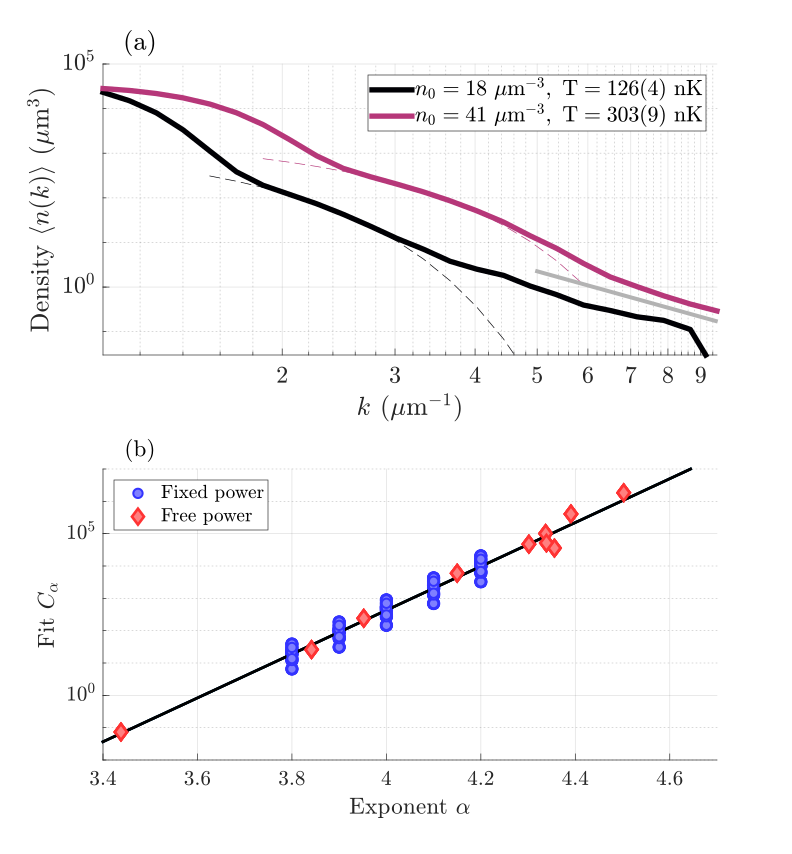
\includegraphics[width=0.5\textwidth]{fig/depletion/exp_density}
	        \caption{The empirical density of particle momenta for two traps (a), where the thermal parts (dashed lines) exponentially decay and give way to the depletion region, marked with grey dashed line proportional to $k^{-4}$.
	        In (b) we illustrate the large hidden systematic errors in a fit to the density which a power law.
	Leaving $\alpha$ as a free parameter gives a wide variation in best-fit exponents and scale coefficients.
	Blue squares show the amplitude coefficient $C_\alpha$ given a fixed exponent $\alpha$ fixed at five values within the range of fit results, applied to all data sets.
	The choice of $\alpha$ powerfully determines the coefficient $C_\alpha$, but the error bars (standard errors in fit parameters) are smaller than the markers in all cases.}
	        \label{fig:contact_determination_issues}
	\end{figure}


	In Fig.
	\ref{fig:contact_determination_issues} (a) we show the empirical density $n(k)$ for two data collection runs at the extreme values of $n_0$ we used.
	The three regimes of the condensate, thermal depletion, and quantum depletion span over five orders of magnitude in density.
	The thermal part of the distribution is well fitted by the momentum distribution of an ideal Bose gas,
	\begin{equation}
		n_T(k) =\frac{N_T}{\zeta(3)} ~\left(\frac{\lambda_{dB}}{2\pi}\right)^3 g_{3/2}\left(\exp\left(-\frac{k^2 \lambda_{dB}^2}{4\pi}\right)\right)
		\label{eqn:th_fun}
	\end{equation}
	wherein the thermal de Broglie wavelength $\lambda_{dB} = \sqrt{2\pi\hbar^2/(m k_B T)}$  yields an estimate of the temperature $T$ which ranges from 100 to 320 nK in our experiments.
	Here, $g_{3/2}(\cdot)$ is the standard Bose integral, $\zeta(\cdot)$ is the Riemann zeta function, and $N_T$ is the number of atoms in the thermal part.
	The thermal population decays exponentially with $k$, and hence cannot account for the counts we observe beyond $k\gtrsim 6~\micron^{-1}$.
	
	In rest of this section we present evidence in support of the identification of these counts with the quantum depletion.
	
	First, though, we show that the otherwise ubiquitous approach of a least-squares regression with a density function is inappropriate in this context.

\subsubsection{Issues with analysis of power laws}	
\label{sec:pow_issues}

	Proceeding with a routine fit of the $k$-space histogram with an additional term of the form $C/k^\alpha$ would appear to be an unobjectionable way to estimate the parameters of the purported quantum-depleted tail.
	However, fitting histograms with power laws is prone to return biased estimates of parameters and to drastically under-report uncertainties, especially when data is available over less than a couple of decades of dynamic range \cite{Clauset09,Virkar14}.
	
	As the authors of \cite{Clauset09} note, ``In practice, we can rarely, if ever, be certain that an observed quantity is drawn from a power-law distribution.
	The most we can say is that our observations are consistent with the hypothesis that $x$ is drawn from [a power law]"
	In this section, we demonstrate some of the problems with a least-squares regression using our data as a case study.
	In the next section we discuss our alternative approach and the inherent limitations of analysing data of this nature.
	
	If we augment the fit function (Eqn.
	(\ref{eqn:th_fun})) with power-law term and leave $\alpha$ as a free parameter, the average exponent of over all runs is 4.2(4).
	
	For comparison, the prior work \cite{Chang16} reported power-law tails with an exponent 4.2(2).
	At first glance, one could simply determine the amplitude of the tails by fixing the exponent to 4, and perhaps achieve better results by using a fit weighting proportional to $k^4$.
	 
	Indeed if we do so, we find an average $C_{\alpha=4}$ which is approximately 8(2) times greater than the coefficient of Eqn.
	(\ref{eqn:pred_scaling}), and in general agreement with ref.
	\cite{Chang16}.
	However, there are issues which undermine the reliability of this otherwise standard approach.

	First, in Fig.
	\ref{fig:contact_determination_issues} (b) we illustrate how the choice of scaling exponent $\alpha$ leads to an exponential change in the scale coefficient $C_\alpha$ that one obtains from fitting to a fixed dataset.
	The coefficient $C_\alpha$ varies over about three orders of magnitude \emph{either way} as one uses different exponents $\alpha$ which lie within the range of uncertainties reported here and in the prior work \cite{Chang16}.
	
	Furthermore, this problem is not reflected in the error estimates in the fitting routines: The error bars representing the uncertainty in fit amplitude are smaller than the markers used in Fig.
	\ref{fig:contact_determination_issues} (b).
	
	A linear fit shows that $d \log_{10} C/d\alpha \approx 6.8$, from which we can infer the exponent that would yield an amplitude in good agreement with Eqn.
	(\ref{eqn:pred_scaling}).
	
	This turns out to be approximately 3.9, which lies within one standard deviation from the mean exponent obtained from the regression we just described.
	
	Conversely, we can estimate that the best-fit exponents reported in the prior work would lead to scale coefficients a factor of about 23 greater than their conclusions, and the associated variance could be even larger.
	It is easy to see that a well-intentioned choice of $\alpha$, which is not statistically different from the best-fit estimates, can lead to  conclusion which either agrees perfectly or disagrees catastrophically with the predictions of Eqn.
	(\ref{eqn:pred_scaling}).
	In particular if one assumes that the data conforms to a power law with $\alpha=4$, one is forced to conclude that the Tan theory is wrong, but the inherent -- hidden -- uncertainty in this approach precludes the possibility of such a definitive statement.


	Second, a deceptively reassuring result can be found by multiplying the empirical density by $k^4$, observing a flat region, and adding a constant term in an appropriately scaled model of the thermal region (i.e.
	Eqn.
	(\ref{eqn:th_fun}) multiplied by $k^4$).
	
	In fact, this offers no recourse from the issues described above and is not a definitive test for the presence of a power law or a way t obtain its parameters.
	Suppose the density decays as some $C k^{-(\alpha+\epsilon)}$: then following the rescaling operation $k^\alpha n(k)$, one then has a density which would be expected to be have the form $C k^{-\epsilon}$.
	
	A variation in the (true) $\alpha$ within the systematic variation above leads difference of a factor of $O(2^{0.1})\approx1.07$ over the range $5\micron^{-1}\lesssim k\lesssim10\micron^{-1}$ range reported here and in \cite{Chang16}.
	This variation is dominated by the statistical fluctuations arising in the individual density profiles from random sampling, and is not distinguishable from the run-to-run variation in the power law.
	
	Despite this, fitting such a weighted distribution is similarly sensitive to the choice of weighting function
	For example, fixing the fit exponent at $\alpha=4$ and changing the \emph{weighting function} (not the form of the fit) in the fit from $k^4$ to $k^{4.1}$ returns a coefficient different by a factor of ten.
	This points to one of the primary challenges with power laws; the exponent are strongly entwined with the rate of occurrence of rare events, which by definition are subject to large statistical errors and thus subvert even the most meticulous investigations.

	In sum, these problems with fitting power laws are ubiquitous, and made more difficult by the small range of $k$ which are visible in the helium experiments.
	In general, estimating the exponent of a purported power law is difficult and requires data spanning several orders of magnitude in scale \cite{Goldstein04,Clauset09,Virkar14,Hanel17}, which are not present in either helium experiment.
	The preferred statistical tools for analysing power law distributions are maximum likelihood estimators, as discussed in lucid terms in Refs.
	\cite{Clauset09,Virkar14}.
	However, in these particle detection experiments the limited sampling region and presence of spurious detection events (described below) mean that such estimators are not appropriate.
	In the next section we describe an alternative approach which does not require -- and conversely cannot determine -- a precise value of the scaling exponent.
	We hope this discussion provides the theoretical and experimental community with an understanding of some problems with heavy-tailed distributions and points the way towards a sound analysis of such phenomena in future works.
	 % which neither assumes the data conforms to the theory under test nor requires precise determination of the exponent of the power law.
	
	
	\begin{figure}[t]
	\begin{center}
		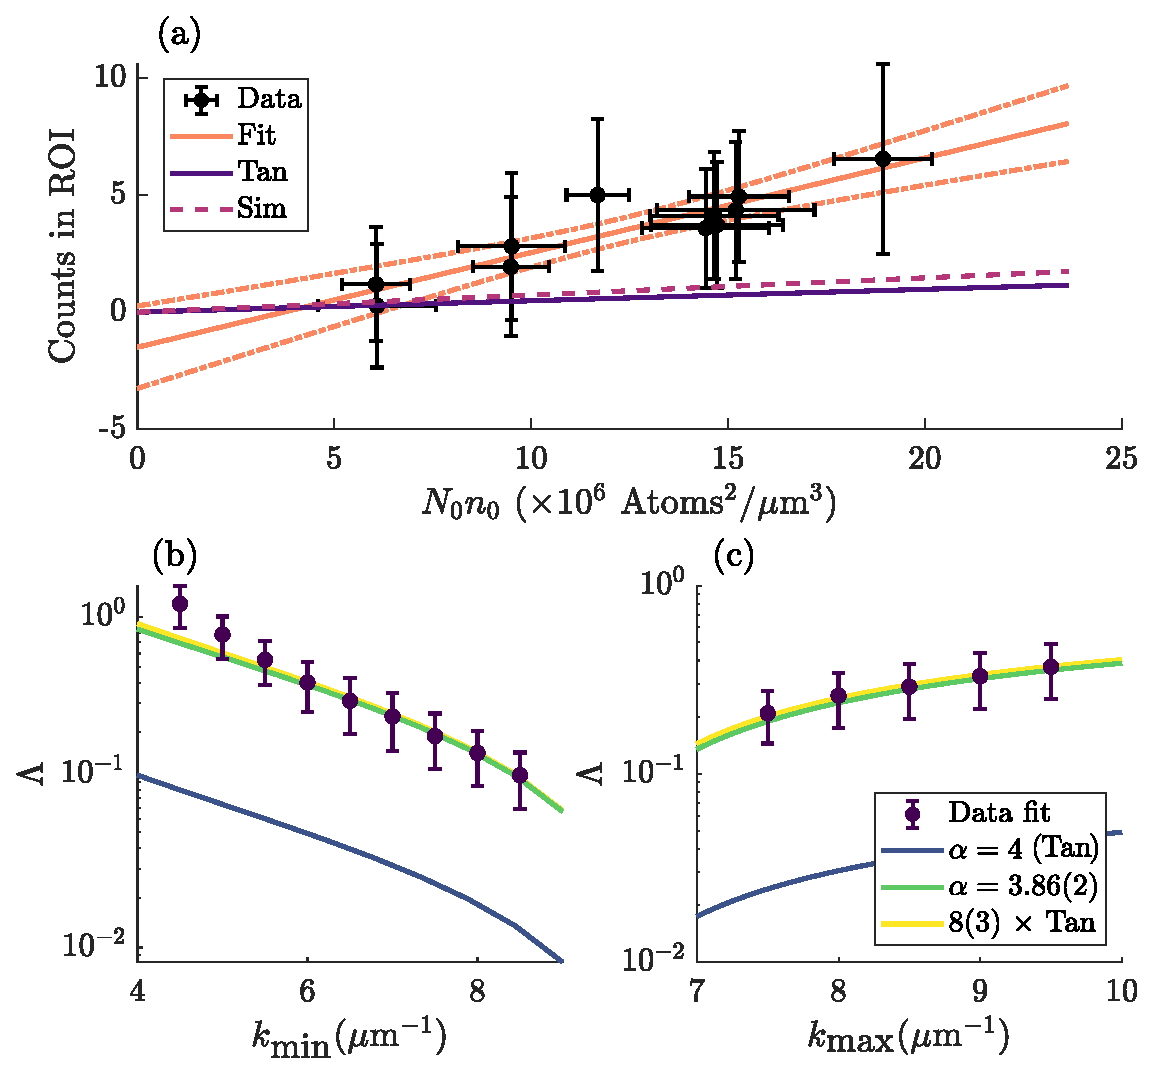
\includegraphics[width=\columnwidth]{fig/depletion/exp_results}
			\caption{A linear fit (a) shows that the product $N_0n_0$ is a good predictor of the number of counts within a region $(k_\textrm{min},k_\textrm{max})$, consistent with Eqn (\ref{eqn:pred_scaling}).
	The gradient $\Lambda_\textrm{fit}$ can be predicted using Eqn (\ref{eqn:pred_scaling}) but the two results disagree by a factor of about 8.
	The number of counts, hence $\Lambda$, depend on the choice of $k$ bounds, as shown in (b,c).
	This dependence does not provide estimates of $C$ or $\alpha$ because multiple hypotheses can produce indistinguishable behavior.
	In (b,c) we show predictions based on Eqn (\ref{eqn:pred_scaling}), along with the predictions of a density function $n(k)$ that is approximately 8(3) times Eqn.
	(\ref{eqn:pred_scaling}) and one that has exactly the amplitude $\mathcal{C}$ but a modified exponent.
	In (b), the deviation from the predictions at $k_\textrm{min}\lesssim6~\micron^{-1}$ is because the collection area starts to overlap with the thermal region.
			}

		\label{fig:exp_results}
	\end{center}
	\end{figure}

\subsubsection{Testing Tan's Tails}

	The prediction of the momentum tail shape (via Eqn.
	(\ref{eqn:pred_scaling})) captures a great deal of information, which can be split into two independently testable hypotheses.
	
	The first claim which we test is that the amplitude of this tail scales in proportion to the product $n_0 N_0$, and the second is the exponent of the density decay.
	Under the null hypothesis that the \emph{in situ} depletion survives the expansion and escapes the condensate undisturbed, one can integrate Eqn.
	(\ref{eqn:pred_scaling}) to predict the number of atoms whose wavevector has a modulus in the interval $k\in (k_\textrm{min}, k_\textrm{max})$, 

	\begin{equation}
		N_{k_\textrm{min},k_\textrm{max}} =\frac{\mathcal{C}}{2\pi^2}\left(\frac{1}{k_\textrm{min}}-\frac{1}{k_\textrm{max}}\right)
		\label{eqn:pred_num}
	\end{equation}
	Note that the integral of $n(k)$ is taken with the differential form $(2\pi^{-3})\d\kvec$ in spherical coordinates.
	For fixed $k_\textrm{min}$ and $k_\textrm{max}$, Eqn.
	(\ref{eqn:pred_num}) has the form $N_{k_\textrm{min},k_\textrm{max}} = \Lambda N_0n_0$ (c.f.
	Eqn.
	\ref{eqn:pred_scaling}).
	
	We can test this form directly by measuring the number of counts detected in the interval $(k_\textrm{min},k_\textrm{max})$ after producing a BEC of $N_0$ atoms with peak density $n_0$.
	
	The figure of merit for this description will be the goodness of fit of a simple linear regression.
	
	As above, we choose $k_\textrm{min}=6~\micron^{-1}$ which lies outside the thermal part for all our data sets.
	However, the $k$-space field of view is restricted by the detector radius to $k\lesssim5\times 10^6$ m$^{-1}$ in the $(x,y)$ plane, which is only just sufficient to reach past the edge of the thermal region.
	
	We thus face a tradeoff in the choice of $k_\textrm{max}$, therefore we define the bounds of our region of interest (ROI) by the minimum elevation angle $\phi_c=\pi/3$ rad and an upper bound of $k_\textrm{max} = 10\micron^{-1}$.
	This amounts to an ROI consisting of two vertically oriented conical sections, each with half-angle $\pi/6$, encompassing a total solid angle of $0.13\times 4\pi$ steradians.
	
	We must also account for the detector quantum efficiency of 0.08(2) and state-transfer efficiency of 25(2)\%, and combine all these factors into the total efficiency $\epsilon\approx0.23(5)\%$.
	After we discuss the results of this analysis, we will  examine the (lack of) effect of uncertainty in $\epsilon$ and the choice of $\phi_c$.
	% We find that the observed number $N_\textrm{exp}$ is 
	% Further, a straight line in a log-log plot is far from conclusive evidence of a power law as there exist other distributions (such as the log-normal and exponential distributions) which also present this way over larger domains than resolved in either of the helium experiments.	
	
	
	% Fixing the power at 3.86 yields 0.8(2) times the predicted contact
%     And at the 95% CI 
%         3.84 0.6(2) times Tan
%         3.88 1.1(3) times Tan
%     But it's not clear what this would mean, physically speaking...
%     so that would be approx 0.8(3) times Tan theor


	A linear fit of the form $\hat{N}_{k_\textrm{min},k_\textrm{max}} = \Lambda_\textrm{fit} n_0 N_0 + c$ yields a vertical intercept $c$ consistent with zero (c=-0.9,  95\% CI (-3.1, 1.2)) and a good correlation ($r^2\approx0.8$, $p=1\times10^{-3}$), providing evidence supporting the expected linear relationship.
	
	The correlation coefficient between the (normalized) variables $N_\textrm{exp}$ and $N_0n_0\propto(N_0^7\bar{\omega}^6)^{1/5}$ is 0.9.
	We conclude that the product $N_0n_0$ is a predictor of the depleted population, which is consistent with Eqn.
	\ref{eqn:pred_scaling}.
	We tested other combinations of the independent variables and found no physically-motivated combination provides a better fit.
	For comparison, a linear fit proves that the atom number itself is a poor predictor of the detected number ($r^2=0.05~,p=0.54$), as is the density alone ($r^2=0.4~,p=0.04$).

	The gradient $\Lambda_\textrm{fit}$ is of particular interest because it can be predicted using Eqn.
	\ref{eqn:pred_num}.
	Given an ROI, one can calculate $\Lambda_\textrm{pred} = 32 \epsilon a^2(k_{\textrm{min}}^{-1}-k_{\textrm{max}}^{-1})/7$.
	We find that the predicted slope disagrees with the empirical fit by a factor of $\Lambda_\textrm{fit}/\Lambda_\textrm{pred}= 8.3$, 95\% CI $(5.5,11)$.


	We are then tasked with reconciling the nonlinear scaling of the detected counts, which is consistent with the quantum depletion, and the disagreement over the absolute number of detected counts.
	We may look to understand the disagreement in terms of the deviation from Eqn.
	(\ref{eqn:pred_scaling}).
	We focus on the two most parsimonious alternatives: whether the tail amplitude is simply larger than expected (i.e.
	$n(k)=A\mathcal{C}/k^4$), or whether the tail decay is somehow modified (i.e.
	$n(k)=\mathcal{C}/k^{4+\delta})$.
	The former would imply that the derivation using the sweep theorem (or Bogoliubov theory in a local density approximation \cite{Chang16}) misses something essential about the system.
	The latter could point to some physical effect, either analogous to the prethermal dynamics of unitary gases \cite{Makotyn14,Eigen18,Colussi20,Kira15_coherent,Smith14} or another factor particular to the dilute regime.
	
	Ultimately, such a distinction between these hypotheses is not possible given the data at hand.
	
	% Specifically, through the appearance of the $k$ boundary values in Eqn.
	\ref{eqn:pred_num}, one could look to the $k$-depndence of $\Lambda_\textrm{pred}$ for a test of the density \emph{ansatze} above.
	Specifically, the density profiles $n(k)=A\mathcal{C}/k^4$ with $A=8(3)$ and $n(k)=\mathcal{C}/k^{\alpha}$ with $\alpha=3.86(2)$ both predict the variation of $\Lambda_{pred}$ with $k_\textrm{min}$ and $k_\textrm{max}$ with comparable accuracy (Fig.
	\ref{fig:exp_results} (b,c)).
	% In other words, if one insists on fitting a distribution of the form $k^{-4}$ then one concludes that the prediction for $\mathcal{C}$ is wrong by a factor of 8(3).
	It is thus not possible to tell whether we have a tail with the expected exponent but a greater weight, or the correct weight but a slower decay, or some combination of the two.
	% Indeed, the space of possible alternative hypotheses is practically infinite: One could find equally-apt distributions by modifying the power and coefficient together.
	Without the ability to precisely determine the exponent $\alpha$, there is insufficient evidence to conclude which of these is correct, therefore little can be said with certainty about which aspect of Eqn.
	(\ref{eqn:pred_scaling}) is incorrect or what physical effects might underpin this disagreement.
	Indeed, the predicted $k^{-4}$ behaviour is only a strict constraint inasmuch as it can be shown to persist (exactly) after the expansion, which as we argued above is not feasible, and argue below is not necessarily expected.
	One conclusion remains robust: There are about ten times as many detections in the depletion region as one would expect based on the Tan theory.
	
	Later in this section we provide technical details of our experiments and rule out several systematic factors which could lead to this disagreement.

	% Although our method provides a direct test of one aspect of Eqn.
	(\ref{eqn:pred_scaling}), it does not circumvent the fundamental challenges of analysing power laws.
	

	Nonetheless, the particular nonlinear scaling of detected counts with the predictor $N_0n_0$ is concordant with the tails' originating in the quantum depletion.
	Furthermore, our simulations indicate that the quantum depletion can survive the condensate expansion, presenting depleted tails in the far-field with modified amplitude.
	
	We are therefore faced with the conclusion that tails are indeed a signature of quantum depletion, albeit subject to some effect during expansion into which the present analysis can see no further.
	Given the similarity in settings and findings, the same could be said for the prior work \cite{Chang16}.
	% Comparing our work to \cite{Chang16}, given the similarity between experiments and consistency of the regression results above, our work can be said to corroborate their findings, albeit withthe prior work appears subject to the same limitations.
	
	
	% Our results could be seen as a count against the interpretation of these tails as a signature of the quantum depletion.
	
	% However, we note two pieces of evidence that give weight to this interpretation.
	
	% First, we are not aware of any other proposed physical effect which exhibits this specific nonlinear scaling relationship with respect to the atom number.
	% Second, we find evidence in our simulations (see below) that the momentum-space signature of the quantum depletion does survive the condensate expansion, and indeed appears in excess of the predicted \emph{in-situ} depletion.
	
	
	


\subsection{Experimental details}
\label{sec:exp_details}
\subsubsection{Trap configuration}

	We prepared our BECs with via forced evaporative cooling in a harmonic magnetic trap with trap frequencies $(45,425,425)$ Hz and a DC bias stabilized by our auxiliary field compensation coils \cite{Dall07,Dedman07}.
	For the tight trap we increased the coil current after the cooling sequence to obtain trapping frequencies $(71,902,895)$ Hz, ramping the field as a sigmoid step function to minimize in-trap oscillations.
	Note that the weak ($x$) axis of the trap is horizontal, with tight vertical confinement.
	The trap remained on for 150ms before switching the trap off with a $1/e$ time of $\approx38\mu$s.
	The condensates were allowed to expand for 2ms before we transferred some of the condensate into the magnetically insensitive $m_J=0$ state via Landau-Zener sweep to prevent distortion by stray magnetic fields.
	The RF pulse was created by a  function generator, amplified, and applied to the experiment chamber by a coiled antenna inserted into the BiQUIC coil housing.
	The pulse swept from 1.6-2.6MHz over 1ms and was centred on the fine structure resonance between the $m_J$ states.
	The determination of the transfer efficiencies $\eta_j$ for each of the $m_J = j$ states is discussed below.
	The sweep was $10^6$-fold wider than the Doppler broadening of the BEC which ensured uniform transfer at all momenta.
	Immediately after the RF sweep, the bias coils are switched off and auxiliary push coils in the vertical (Z) and weak horizontal (X) axes are activated using a fast MOSFET switch to implement a Stern-Gerlach separation of the $m_J = -1,~0,$ and $+1$ pulses.

	We use a Roentdek DLD80 multichannel plate and delay-line detector stack \cite{Manning10} located 859mm below the trap, which registers the arrival times and positions $(t_i,x_i,y_i)$ of each atom, indexed by $i$.
	
	The velocity of each atom relative to the centre of mass of each cloud is calculated by $(v_x,v_y,v_z) = t_{i}^{-1}(x_i-\bar{x},y_i-\bar{y},g_0(\tau^2-t_{i}^{2}))$, where $g_0$ is the local gravitational acceleration and the overbar denotes the within-shot average and $\tau$ ms is the time of flight of the centre of mass of the cloud.
	
	The far-field momentum is thus obtained via $m\textbf{v} = \hbar\kvec$.
	The velocity conversion assumes a point source but carries a negligible error of a few ppm as the in-trap BEC size is smaller than the detector resolution.
	
	The space and time resolution of the detector are 100 $\mu$m and 3 $\mu$s, respectively \cite{Henson18}, and the detector efficiency of $8(2)\%$ was determined from the collection efficiency of correlated atoms on the opposite sides of scattering halos \cite{shin19,shin20,Jaskula10}.
	

	\com{While the determination of the factor $\epsilon$ is important, the dominant uncertainty is the 25\% error in the detector efficiency.
	The collection area cutoff $\phi_c$ also factors in but this is precisely known.
	
	We performed the analysis described above for a range of $\phi_c$ and values of the QE and found that the excess of counts (expressed as $\Lambda_\textrm{fit}/\Lambda_\textrm{pred}$) was not significantly effected, which we summarize in Tab.
	\ref{tab:choice_indep}.}

	\begin{table}[b]
		\begin{tabular}{c c c c}
			\hline\hline
			% $k$ lim.
	($\micron^{-1}$) & fit $r^2$ &  $\Lambda_\textrm{fit}$ & $\Lambda_\textrm{fit}/\Lambda_\textrm{pred}$\\  
			% \hline
			% (6,7)  &  0.88     & 0.2(0.1,0.2) &   9.1(6.5,11.7)\\
			% (6,8)  &  0.85     & 0.3(0.2,0.3) &   8.4(5.7,11.1)\\
			% (6,9)  &  0.83     & 0.3(0.2,0.4) &   8.1(5.3,10.8)\\
			% (7,10)  &   0.79     & 0.2(0.2,0.3) &   7.8(4.8,10.8)\\
			% (8,10)  &   0.79     & 0.1(0.1,0.2) &   8.0(4.9,11.2)\\
			% \hline
			QE & fit $r^2$ &  $\Lambda_\textrm{fit}$ & $\Lambda_\textrm{fit}/\Lambda_\textrm{pred}$\\      
			\hline
			0.05    &   0.83   &   0.2(0.1,0.3)  &  6.8(4.5,9.1)\\
			0.06    &   0.83   &   0.3(0.2,0.4)  &  7.4(4.9,9.8)\\
			0.07    &   0.83   &   0.3(0.2,0.4)  &  7.8(5.2,10.5)\\
			0.08    &   0.83   &   0.4(0.3,0.5)  &  8.3(5.5,11)\\
			0.09    &   0.83   &   0.5(0.3,0.6)  &  8.7(5.8,11.6)\\
			0.1     &   0.83   &   0.6(0.4,0.7)  &  9.0(6.0,12.1)\\
			0.11    &   0.83   &   0.6(0.4,0.8)  &  9.4(6.2,12.5)\\
			\hline
			Half-angle & fit $r^2$ &  $\Lambda_\textrm{fit}$ & $\Lambda_\textrm{fit}/\Lambda_\textrm{pred}$\\
			\hline
			10$^\circ$    &   0.82   &   0.1(0.0,0.1) &  9.3(6.0,12.7)\\
			20$^\circ$    &   0.86   &   0.2(0.1,0.3) &  9.2(6.4,12)\\
			30$^\circ$    &   0.83   &   0.4(0.3,0.5) &  8.3(5.5,11)\\
			\hline\hline
		\end{tabular}
		\caption{The uncertainty in the detector quantum efficiency (QE) does not have a significant effect on the findings.
	Re-running the analysis using different QE yields fits that barely differ in the goodness of whose gradients do not significantly change.
	We also find that the choice of collection area has a weak effect, below statistical significance, on the result.
	Terms in brackets are the upper and lower 95\% confidence intervals.}
		\label{tab:choice_indep}
	\end{table}
	 % we show in Tab.
	\ref{tab:choice_indep}, this has no significant effect on the conclusion (namely, on the comparison $\Lambda_\textrm{fit}/\Lambda_\textrm{pred}$)
	% This could affect the outcome in two ways, first by changing the value of $\chi$ used in the prediction, and second through the factor of $N_{0}^7/5$ used to compute the condensate density $n_0$.
	



\subsubsection{Peak density calibration}

    The quantum depletion and contact are both predicted to depend solely on the condensed number and trapping frequencies via the condensate density, hence it is important to determine both quantities accurately.
	
    % In the Thomas-Fermi approximation, the peak density of the condensate can be written as $n_0 = \mu/g$, where $\mu$ is the chemical potential, $g=4\pi\hbar^2a_{1,1}/m$ is the effective interaction strength, $m\approx6.6\times10^{-27}$ kg is the atomic mass, and $a=7.512$ nm is the s-wave scattering length between pairs of atoms in the $m_J=1$ state \cite{Moal06}.
	
    The sole experimental parameters in the expression for the peak density (Eqn.
	\ref{eqn:n0}) are the geometric trap frequency $\bar{\omega} = \left(\omega_x\cdot\omega_y\cdot\omega_z\right)^{1/3}$, and $N_0$, the number of atoms in the condensate.
	
    We simultaneously determine the total atom number $N$ and trap frequency $\bar{\omega}$ in a single shot using a pulsed atom laser and use the thermal fraction (as below) to determine the condensed number $N_0$.
	

	The pulsed atom laser consists of a series of Fourier-broadened RF pulses centred on the minimum Zeeman splitting in the trap.
	
	The pulse transfers atoms in the trap to the untrapped $m_J=0$ state with an approximately constant transfer rate across the cloud.
	
	We outcouple approximately 2\% of the atoms per 100$\mu$s pulse for $\approx$200 pulses, which eventually depletes the entire trap.
	
	The atom laser thus prevents the detector from saturating and allows an accurate determination of the atom number, up to a factor of the quantum efficiency.
	
	We determine the trapping frequencies by inducing centre-of-mass oscillations with a magnetic impulse, and find the oscillation period from the atom laser pulses \cite{henson18ML}.


\subsubsection{Determining spin transfer efficiency}

	To calibrate the transfer efficiencies, we applied a weaker Stern-Gerlach than for the depletion measurement, resolving each $m_J$ cloud on the detector, as illustrated in Fig.
	\ref{fig:frac_cal}.
	

	\begin{figure}[!t]
	\begin{center}
		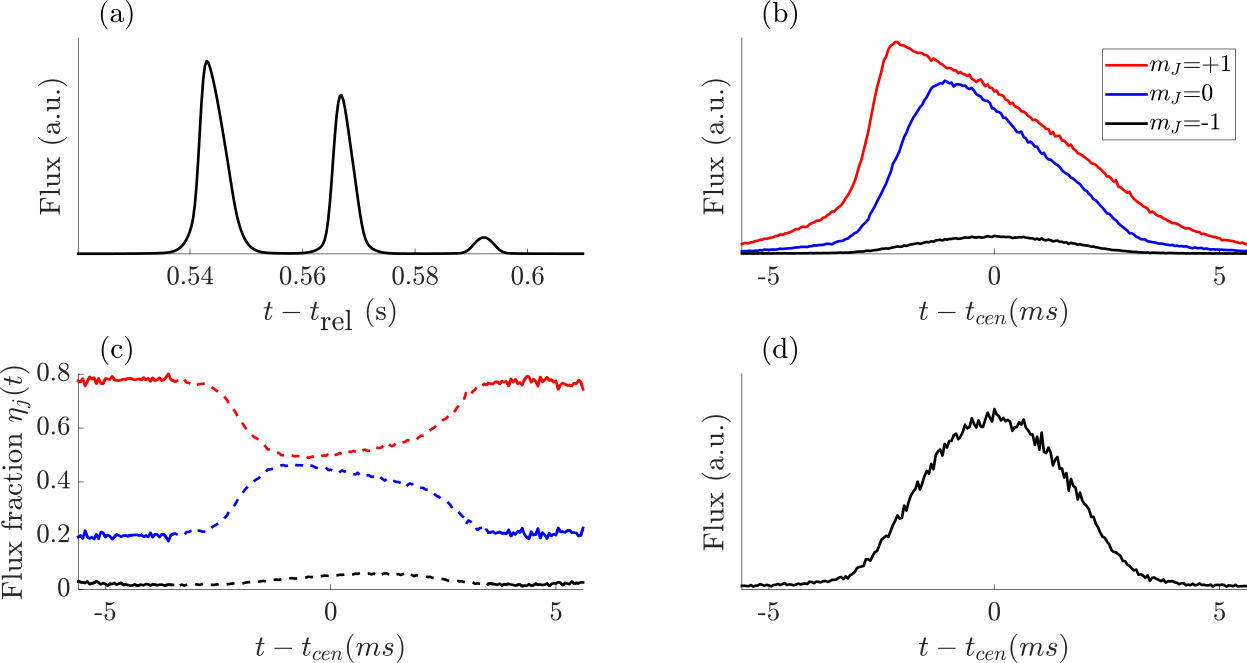
\includegraphics[width=\columnwidth]{fig/depletion/frac_cal_profile}
		\caption{Determining the RF transfer efficiency.
	The time-of-flight profiles of each pulse are resolved (a) by applying a weak Stern-Gerlach pulse during the time of flight.
	The pulses are aligned with respect their centre-of-mass (b) and used to determine the pointwise fraction ((c), dotted line).
	Detector saturation is evident in the peaks (dashed lines), but not in the thermal tails (solid lines), which are used to compute the transfer efficiency.
	Because of its lower flux, the $m_J=-1$ pulse does not show evidence of saturation (d) and is used to determine the thermal fraction.}
		\label{fig:frac_cal}
	\end{center}
	\end{figure}

	The efficiencies $\eta_J$ cannot be calculated by counting the atoms in each cloud because the detector saturates during the peak condensate flux, but we can compare the thermal parts.
	
	We align each cloud along the time (Z) axis and compute the pointwise fraction of the atomic flux $\phi(t)$ accounted for by each cloud, $\eta_j(t) = \phi_j(t)/\sum_j\phi_j(t)$, as depicted in Fig.
	\ref{fig:frac_cal}.
	
	The ratio of densities between the clouds is roughly constant in the thermal part, indicating the absence of important saturation effects and a spin transfer that is independent of $k$.
	
	The fraction of the original cloud transferred into each $m_J$ state is determined by taking the average $\langle\eta_j(t)\rangle$ over the thermal tails.
	
	We find these efficiencies are approximately 74\%, 24\%, and 2\% in all runs for the $m_J=+1$, 0, and -1 states, respectively.
	
	While the $m_J=0$ and $m_J=1$ clouds clearly saturate the detector, the small fraction ($\approx2\%$) of the atoms transferred to the $m_J=-1$ state does not (Fig.
	\ref{fig:frac_cal} (d)).
	
	A bimodal fit to the condensed and thermal parts, plus constant background, yields the thermal and condensed fractions.

	% \com{After a 2ms expansion the cloud is even more dilute than the trap, with a peak density that has approximately halved.
	Therefore the Because the contact in a mixed-species condensate \cite{Vassen16,Werner12_boson}, even if the condensate were still as dense as the in-trap distribution, the contact is reduced relative to the spin-polarized condensate.
	Considering also the reduced density after 2ms expansion, the production rate of quantum-depleted quasiparticles is expected to \emph{decrease} during this process, hence the observed effect is unlikely to emerge at this stage.}
	

% \subsection{Determination of thermal fraction}
	

% 	\begin{figure}[!h]
% 	\begin{center}
% 		\includegraphics[width=0.8\textwidth]{fig/depletion/m1_frac_anal}
% 		\caption{Comparison of thermal fits in the unsaturated $m_J=-1$ pulse including 138 shots.
	The weak (X) and strong horizontal (Y) trapping axes are shown in (a) and (b), respectively.
	\org{would be helpful to label $v_x$ and $v_y$ to make it self-evident at 1st glance.} Both projections display a bimodal peak, with the condensate (dotted lines) and thermal parts (thick solid lines) easily distinguished.
	Fitting a Gaussian profile (thin solid line) to the velocity distribution of the thermal part yields the thermal number and temperature.
	Subtracting the fit leaves the condensate profile (c) which can be \blu{\dots something\dots} yields the condensed number.}
% 		\label{fig:thermal_frac}
% 	\end{center}
% 	\end{figure}


\subsubsection{Noise sources}
\label{sec:spinpop}

	In early tests of our measurement sequence we noticed a contamination of the signal by spurious counts.
	
	We inferred these were remnant counts from the $m_J=+1$ cloud as they were still visible when we ran an experimental sequence without the Landau-Zener transfer.
	
	This contamination appeared in a particular region of our detection image, and as such we were able to correct for it by subtracting their contribution from the counts collected during measurement shots.
	
	Generally, fewer atoms can be attributed to this noise than would be required to explain the discrepancy described in the main text.
	
	While the cause of the cross-contamination is unclear, we observe that the count density outside the region of interest is similar in both the shots with the RF pulse and those without.
	
	We hypothesize that the remnant counts are atoms transferred into the $m_J=0$ state by non-ideal behaviour of the Stern-Gerlach pulses.
	
	We note that only about one in a million atoms from the $m_J=1$ cloud present in this manner in a given shot.

	\com{Such counts constitute about 10(5)\% of the detection events in the ROI.
	Because it is not possible to distinguish \emph{which} atoms are spurious and which are genuine quantum-depleted particles, the preferred power-law analysis (the maximum-likelihood estimator) is not available.
	Basic MLEs are built assuming one has a sample drawn from a distribution of a single category; the probabilistic combination of two different sources of events falls outside the scope of this framework.}


% \begin{table}
% 		\begin{tabular}{ccccccc}
% 		\hline \hline 
% 		$n_0$ ($\mu$m$^{-3}$)  & $N_0\times10^{-5}$ & $\eta_\textrm{Th}$ & T (nK) & $N_\textrm{det}$ & $N_\textrm{pred}$ & $N_\textrm{det}/N_\textrm{pred}$ \\ 
% 		\hline 
% 		17(2) & 3.6(3) & 0.09 & 130(20) & 1.2(1) & 0.3(1) & 5(2) \\ 
% 		17(3) & 3.6(6) & 0.08 & 190(20) & 0.3(04) & 0.3(1) & 1(1) \\ 
% 		19(1) & 5.1(3) & 0.18 & 150(10) & 1.9(1) & 0.3(1) & 6(3) \\ 
% 		19(2) & 4.9(5) & 0.09 & 150(10) & 2.8(1) & 0.4(1) & 7(4) \\ 
% 		20(1) & 5.7(2) & 0.1  & 137(9)  & 5.0(1) & 0.5(1) & 10(4) \\ 
% 		39(4) & 3.8(3) & 0.11 & 252(3)  & 3.7(1) & 0.6(1) & 6(4) \\ 
% 		39(4) & 3.9(3) & 0.11 & 268(2)  & 4.4(1) & 0.6(1) & 8(5) \\ 
% 		39(3) & 3.8(3) & 0.1  & 249(3)  & 4.1(1) & 0.5(1) & 8(4) \\ 
% 		39(3) & 3.7(3) & 0.09 & 237(3)  & 3.6(1) & 0.5(1) & 7(4) \\ 
% 		39(3) & 4.0(2) & 0.14 & 312(3)  & 4.9(1) & 0.5(1) & 10(5) \\ 
% 		41(2) & 4.6(2) & 0.12 & 302(3)  & 6.6(2) & 0.7(2) & 10(6) \\ 
% 		\hline \hline 
% 		\end{tabular}
% 		\caption{Summary of results for each data run.
	The peak density is determined from measurements of the trapping frequencies and the condensed number (via $N_0=N_\textrm{tot}(1-\eta_\textrm{Th})$, using the total number $N_\textrm{tot}$ and thermal fraction $\eta_\textrm{Th}$).
	The number $N_\textrm{Detect}$ of atoms detected in the region of interest (results shown here for the largest ROI) can be compared to the predictions of the Tan theory, as in the main text.}
% 		\label{tab:run_results}
% 	\end{table}

	


	

% \subsubsection{Barriers to employing MLEs}

% 	The presence of these counts is one factor preventing a straightforward application of a maximum-likelihood estimator (MLE) to determine parameters of the power-law region.
	
% 	The basic principle of the MLE is to assume a functional form for the probability distribution $p(x|\theta)$ underlying the observed data $x$, and dependent on some parameters $\theta$.
% 	The zero of the derivative of the \emph{likelihood} function $L(\theta|x)$ with respect to the parameters $\theta$ then yields the most-probable parameter values given a set of observations $x$.
	
% 	In our context, one can assume a functional form for the probability distribution underlying atomic detection events (via a wavefunction ansatz).
	
% 	The detector dark counts can also be incorporated by assuming a uniform distribution, although this entails a cumbersome procedure to retain proper normalization.
% 	However, the dark counts present less than one detection per shot, on average, and thus might be ignorable without major consequence.
% 	The major obstacle to implementing an MLE is the finite detection region.
	
% 	Specifically, because the normalization condition 
	

%     \begin{figure}[!b]
% 	\begin{center}
% 		\includegraphics[width=\columnwidth]{fig/depletion/spinpop}
% 		\caption{Measured contribution of the detector dark counts and spurious spin counts to the time-of-flight profile.
% 	We accounted for the pulse at around 550ms and subtracted it from the measured profiles when computing the contact.
% 	After removing this background term, the density profiles above and below the condensate agree, indicating convergence on the true signal.
% 	For reference, the peak flux of the $m_J=0$ condensate is about a thousandfold greater than the peak shown here.}
% % 		\label{fig:spinpop}
% % 	\end{center}
% % 	\end{figure}

% % 	\begin{figure}[!h]
% % 	\begin{center}
% % 		\includegraphics[width=\textwidth]{fig/depletion/profile_overlay}
% % 		\caption{Comparison of average time-of-flight profiles over a single data run for the quantum depletion measurement shots (blue, 871 shots), transfer efficiency calibration (black, 112 shots), detector dark counts (red, 871 shots), and spurious counts (dot-dash, 895 shots).
% 	The time window bounded by $|k|\leq 10\mu$m is indicated with dotted lines.
% 	Shaded area is the standard error over the entire run.}
% % 		\label{fig:tof_profile}
% % 	\end{center}
% % 	\end{figure}




% % Note that the temps disagree between axes, but within axes between clouds they are consistent(....ish).
% 	This means we can use the profile ratio method, which is also consistent with comparing the thermal number from the fits.
% % Perhaps comment on the thermal-subtracted part; the TF profile should have a sharp cutoff, but the smooth edges are suggestive evidence of this roll-off

% % \begin{figure}
% % 	\centering
% % 	\includegraphics[width=0.5\textwidth]{fig/depletion/counts_per_run}
% % 	\caption{Number of counts detected in the region of interest in the depletion measurement (a), the spin mixing calibration (b), and the dark count calibration (c).
% 	An average of 3.0(5) counts were detected in the ROI in the spin-mixing calibration shot, and the background count rate was 0.4(2) counts per shot.
% 	Separate lines indicate separate \emph{runs}, i.e.
% 	sequences of shots with fixed parameters.}
% % 	\label{fig:num_counts}
% % \end{figure}








\section{Numerical simulations}
\label{STAB}
	\begin{figure}[b]
	        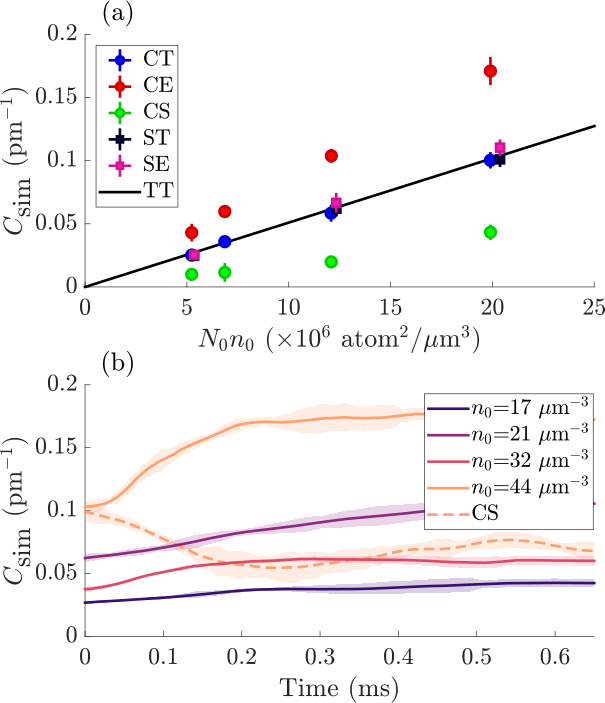
\includegraphics[width=\columnwidth]{fig/depletion/sim_results}
	        \caption{(a) Steady-state values of the simulated contact.
	Simulations of condensates released from a cigar-shaped trap (CT) are consistent with the Tan theory (TT) before release, and show an increase in contact after the trap release (CE).
	A slow relaxation of the transverse trapping frequencies (CS) shows a decrease in line with the predicted value of the lower density.
	Spherical traps (ST,SE) lack any directions of tight confinement, wherein a longer interaction time prevents the escape of depleted particles as seen in cigar traps.
	(b) the time-dependence of the contact stabilizes after a time on the order of $1/\omega_x$, several hundred $\mu$s.
	The difference between in-trap and expanded contact increases with the density of the condensate but is consistently about 1.7 times the Tan theory.
	For comparison, the experimental control pulses are implemented after 2ms of expansion.
	When the transverse trapping frequencies are reduced by half (dotted line), the in-situ contact relaxes.}
	        \label{fig:sim_fig}
	\end{figure}
	We performed simulations of the BEC expansion from harmonic traps using the first principles STAB method \cite{Deuar11,Kheruntsyan12}.
	
	The simulations included a cigar-shaped trap (marked CT in Fig.
	\ref{fig:sim_fig}) with parameters matched to the experimental conditions.
	
	The in-trap state was consistent with the adiabatic sweep theorem before release from the trap.
	
	Following expansion from the cigar trap (CE in Fig.
	\ref{fig:sim_fig})), the simulated tail amplitude increased and stabilized within a few hundred microseconds, much sooner than the 2ms delay between the trap release and application of the rf and Stern-Gerlach pulses.
	
	Fig.
	\ref{fig:sim_fig} shows time evolution of the tail amplitude for the simulated traps using the same ROI as the experimental setup.
	 
	In this configuration the steady-state value of the momentum tails was a factor of 1.64(9) above the predictions of Eqn.
	(\ref{eqn:pred_scaling}).
	

	To understand the disagreement with earlier theory \cite{Qu16}, which predicted no depletion survival, we also investigated the effect of adiabatic expansion on the in-trap depletion by simulating a slow decrease of the transverse trapping frequencies by a factor of two (CS), and found that the in-trap contact decreased roughly as predicted by Eqn.
	(\ref{eqn:pred_scaling}) in these instances --- see the dashed line in Fig.~\ref{fig:sim_fig}.
	
	We also found that the factor of disagreement (i.e.
	$C_\textrm{sim}/C_\textrm{Tan}$) between Eqn.
	(\ref{eqn:pred_num}) and the simulated tails depends on the angle choice of cutoff angle $\phi_c$.
	
	Put another way, the momentum distribution in the simulations is anisotropic and takes the form $f(\theta,\phi)/k^4$ - note that the average of an angle-dependent power law decay preserves the power-law behaviour.
	We find that $C_\textrm{sim}$ is larger for smaller collection regions that are more tightly concentrated about the vertical (strong) trapping axis, whereas larger collection angles (including areas closer to the weak axis) produce a lower $C_\textrm{sim}$.
	In particular, with cone half-angles of 10, 20, and 30 degrees, $C_\textrm{sim}$ was 2.2(3), 1.9(2), and 1.6(1) times $C_\textrm{Tan}$, respectively.
	We note that the experimental results (Tab.
	\ref{tab:choice_indep}) could be said to display a similar trend, but the result is not statisically significant.
	The implementation of the simulations is discussed in detail in the publication \cite{Ross21}.


\section{Discussion}
\label{sec:discussion}

	In sum, we find that the number of atoms in the large-$k$ tails is predicted by the product $N_0n_0\propto(N_{0}^7\bar{\omega}^6)^{1/5}$, in line with Tan's theory of the contact (Eqns.
	\ref{eqn:pred_scaling},\ref{eqn:pred_num}).
	
	However, the sensitivity of this relationship is significantly different than expected by a factor of order 8(3), which is not accounted for by any known systematic effects.
	The method we employ makes a clear distinction between what can and cannot be inferred about the form of the momentum tails, and indeed we find there is no decisive evidence in favour of tails that decay with $k^{-4}$.
	We do note that the prior work \cite{Chang16} reported results which fall within the uncertainty range of our analysis.
	Indeed, Fig.
	4 in \cite{Chang16} could be said to display the relevant scaling with respect to $N_0n_0$ but the reported values of the apparent contact should be considered along with the caveats discussed in Section \ref{sec:pow_issues}.
	
	Taken together with the simulations, our findings show that the survival of the quantum depletion into the far-field is plausible, but not as a straightforward mapping into the far-field density.
	In a non-interacting ballistic expansion, the far-field density distribution would be a direct realization of the in-trap momentum distribution of the cloud.
	
	However, this correspondence is known not to faithful because the dispersal of the mean-field energy into kinetic energy, known as the release energy, imparts some acceleration to the atoms during early expansion.
	
	This effect is responsible for the famous inversion of the cloud aspect ratio upon release from harmonic traps.
	

	As such we interpret our results as an indication that the depleted atoms are accelerated by the non-uniform mean-field energy of the condensate during the expansion.
	In detail, after a quench into the free particle regime, the condensate expands hydrodynamically on timescales of $1/\omega$.
	
	This is an adiabatic process for the low momentum depletion, whereby some depleted atoms are absorbed back into the condensate in agreement with \cite{Qu16}.
	However, the characteristic time for reabsorption is $\hbar/gn_0$, slow enough that quasiparticles in the particle branch of the Bogoliubov dispersion have sufficient velocity to escape the expanding cloud without being reabsorbed and thus transition to free atoms.
	
	This effect leads to the persistence of populated high-$k$ modes in the far-field, which were detected in the experiment.

	Moreover, an atom inside the BEC experiences an effective force from the gradient of the mean-field potential $\textbf{F} = -4\pi\hbar^2 m^{-1}a \nabla  n(x)$.
	
	This endows escaping depleted particles with a greater momentum, increasing the weight of the tails in the far-field.
	
	This effect is exacerbated in light atoms like $^{4}$He, whereas it would be suppressed by a $\sim500$-fold in $^{87}$Rb experiments \cite{Makotyn14} because the acceleration scales with $1/m^2$.
	
	Further, it is much easier for depletion atoms to escape and be accelerated in the transverse x-y directions from an elongated cloud because the distances $R_{TF}=\frac{1}{\omega}\sqrt{2gn_0/m}$ are reduced by $\bar{\omega}/\omega_{x,y}$, whereas the initial mean depletion velocities \textit{in situ} $v\sim \sqrt{2gn_0/m}$ are isotropic.
	Indeed, spherical clouds (SE) exhibit a much weaker effect than the elongated clouds (CE) owing to the longer escape time.
	This also presents as an increase in $C_\textrm{sim}$ for smaller collection regions.
	
	The statistical uncertainty in the experimental findings preclude a definitive comparison on this particular point.

	The interpretation just described is supported by another observation within the simulations:
	During the expansion we observe a decrease in the total number of depleted particles (reabsorption) and a simultaneous increase of the large-k population (forcing).
	
	This constitutes a partial explanation of the experimenal findings too, and results in tail amplitudes which are consistent with the quantum depletion multiplied by a constant factor.
	
	However, a mystery remains: Why is there an excess of particles in the depletion region which is so much greater than accounted for by this picture? 
	This issue should be resolved if far-field observations are to be interpreted in terms of the in-trap physics of interest.
	
	
	As we discussed, our systematic uncertainties are unable to account for the observed excess population of the quantum-depleted tails.
	Futher, despite the ultracold clouds being realized at finite temperatures, the thermal population of quasiparticles cannot account for the observed counts.
	
	The thermal quasiparticles in the Bogoliubov picture simply reflect a change of basis which maps identically onto the thermal population of constituent particles \footnote{See, for example, \cite{PethickSmith} Chap.
	8.3.}.
	
	Quasiparticles whose wavenumber exceeds that of the speed of sound lie within the particle-like branch of the bogoliubov spectrum, which for our considerations is on the order of $k\gtrsim2~\micron^{-1}$, well within the thermal velocities.
	
	Hence, given the exponential decay of thermally populated states, the large-$k$ tails are unambiguously \emph{not} thermal effects.
	

	In conclusion, our work expands the growing suite of far-field investigations of quantum depletion \cite{Cayla20,Chang16} and confirms that quantum depletion can, remarkably, survive past the lifetime of its original condensate.
	
	Our simulations clarify how the depletion can be visible in the far-field momentum distribution here and in earlier experiments, and that the hydrodynamic approximation does not capture sufficient short-wavelength information to make detailed predictions about the high-momentum behaviour.
	
	We thus find a partial explanation for the deviation of the far-field distribution from both the predicted in-situ depletion and the hydrodynamic reabsorption: The interplay between coherent absorption of Bogoliubov excitations and the dispersal of the chemical potential into kinetic energy, to which helium is particularly sensitive, result in a growth of the $k^{-4}$ tails of the momentum distribution during freefall.
	

	It would be informative to determine whether the outstanding discrepancy originates in the trapped condensate or is due to some unknown non-equilibrium effect during expansion.
	This question invites complementary studies of the \emph{in situ} depletion in \mhe BECs.
	
	Such an investigation requires an \emph{in situ} probe of the contact, such as RF spectroscopy or Bragg spectroscopy.
	The latter may be the most fruitful of the two simply because of the difficulty of interpreting the results from the former, which we sketch here.
	
	
	The basic principle of RF contact spectroscopy is to apply a monochromatic RF probe which is detuned from the resonance between two spin states, coupling atoms in the initial spin state to an untrapped channel.
	
	One then performs a differential measurement of the atom number and expects the signal strength to scale as $\omega_\textrm{RF}^{3/2}$ with the detuning from the RF resonance.
	The loss rate is also proportional to the difference of reciprocal scattering lengths $\Gamma\propto(1/a_\textrm{i,i}-1/a_\textrm{i,f})$ between pairs of atoms in initial-initial ($a_{i,i}$) and initial-final ($a_{i,f}$) spin states \cite{Braaten10,Wild12}.
	
	For He$^*$ (spin 1) the scattering lengths $a_{1,1}$ and $a_{1,0}$ are identical \cite{Leo01}, rendering the preferred $m_J=1-m_J=0$ transition unusable.
	
	On the other hand, $a_{1,-1} = 3/7 a_{1,1}$ \cite{Vassen16}, and the singlet transition can be driven without populating the $m_J=0$ state.
	
	In principle this could produce a detectable flux of atoms to perform sensitive in-trap contact measurements, however, collisions in the $^1\Sigma_{g}^{+}$ channel have large Penning ionization rates which lead to significant trap losses \cite{Leo01}.
	
	The ionization products would be detectable by in-vacuum channel electron multipliers but require theoretical work to disentangle from the spectroscopic signal.
	
	Further, while other atomic species offer Feshbach resonances by which to tune the inter-species scattering length (and hence signal or ionization rate), \mhe has no such feature.
	
	While such a measurement is not \emph{prima facie} impossible, Bragg spectroscopy may yield more readily interpretable results.



% \begin{abstract}

% Measurements of Tan's contact in expanding condensate conflict with predictions of the \emph{in situ} quantum depletion.
	% It is unclear how the depletion survives without a condensate, and even appears stronger in the far-field than before the trap release.
	% We confirm experimental observations of a slowly-decaying tails in the far-field, consistent with the survival of the quantum depletion.
	% Simulations of our experiment support shed light on the mechanisms behind the observations.
	% A gap between the numerical and empirical results remains an open question obstructing studies of quantum depletion in the far field.
% % max 600chars for PRL
% % \end{abstract}

% % \maketitle

% \section{Introduction} 
% 	The mechanism underlying superfluid formation is the Bose-Einstein condensation of collective excitations.
	
% 	This was formalized by Bogoliubov’s transformation \cite{Bogolubov47} of a homogeneous system of interacting bosons into a free Bose gas of collective excitations constituted by oppositely-moving particles \cite{Vogels02}.
	
% 	In a superfluid, the macroscopically-occupied quasiparticle ground state corresponds to the superfluid part, and population of excited quasiparticle modes constitute the normal component of the fluid.
	
% 	This foundational theory is of broad relevance because the BEC and BCS regimes of superconductivity are characterized by superfluids of molecular dimers and of Cooper pairs, respectively.
	  

% 	Interactions between constituent particles lead to a zero-point population of quasiparticle modes, known as the quantum depletion, which persists even at zero temperature.
	
% 	The quantum depletion presents as an occupation of single particle modes with large momentum $p$ that decays like $p^{-4}$.
% 	In liquid helium, the depleted fraction is large (of order 90\% of the fluid) due to the strong interparticle interactions, but is generally very small in weakly-interacting dilute gases.
% 	Bogoliubov's theory makes accurate predictions of the total depleted population in ultracold atomic Bose-Einstein condensates (BECs) \cite{xu06,lopes17_depletion} and exciton-polariton condensates in solid substrates \cite{pieczarka20}.
% 	Therefore, detailed study of the quantum-depleted tails of the momentum distribution in ultracold gases is an attractive test for the Bogoliubov theory.

% 	This has been challenging to date because the tails are usually beneath the noise floor of optical imaging techniques.
	
% 	A previous experiment \cite{makotyn14} sought to use a Feshbach resonance to produce a visible depleted fraction, but found that the momentum distribution saturated during expansion and did not display a power-law tail.
	
% 	% \com{This was because complex three-body effects play an important role in the pre-thermalization dynamics, and so the asymptotic momentum distribution is no longer characterized purely by two-body dynamics.
	% \cite{kira15_hyperbolic,kira15_coherent}}
% 	In contrast, another experiment found unexpectedly large momentum tails in the far-field of a weakly interacting helium BEC released from a harmonic optical trap \cite{chang16}.
	
% 	This is particularly surprising because conventional wisdom argues that the density decreases adiabatically during expansion, justifying treatment with a hydrodynamic approximation wherein the tails are predicted to vanish \cite{qu16}.
	

% 	These observations are also in conflict with anither successful and widely applicable theory of contact interactions developed by Tan \cite{tan08_energetics,tan08_momentum,tan08_virial}.
% 	The thermodynamic quantity called the \emph{contact} characterizes how s-wave contact interactions modify the short-range pair correlation function.
	
% 	A defining feature of the contact is that it determines the amplitude of the power-law decay of the momentum density in terms of the gas density and s-wave scattering length, which fully determine collisional dynamics in ultracold dilute gases.
	
% 	Two central properties of the contact, known as the adiabatic sweep theorem and generalized virial theorem \cite{tan08_momentum,tan08_virial}, have been verified via radio spectroscopy \cite{baym07,punk07,braaten10} of degenerate Bose \cite{wild12} and Fermi gases \cite{stewart10,sagi12}.
	
% 	While the Bogoliubov prescription breaks down in strongly-correlated systems \cite{lopes17_quasiparticle}, Tan’s theory applies for arbitrary spin mixtures at any density, temperature, and geometry, and both theories are consistent in the weakly interacting regime.

% 	Thus, it is surprising that the prior work observed such strong tails as this contravenes both the Tan and Bogoliubov theories in the weakly-interacting regime where both have otherwise been demonstrated to be accurate.
% 	This implies that either some feature of harmonically trapped helium condensates violate the minimal assumptions of both theories, or that far-field momentum measurements are not a straightforward means of examining the quantum depletion even in weakly interacting gases.
	
% 	It is important to verify and overcome this obstacle, as far-field measurements play a central role in study of ultracold gases.
	

% 	To this end, we revisit the measurement of the momentum distribution of a helium condensate expanding from a harmonic trap.
	
% 	We conducted experiments using a different apparatus and analysis, covering a range of densities twice as large as the prior work, and use a magnetic trap in place of an optical dipole trap which ensures perfect spin-polarization of the condensate.
	
% 	We observe tails in the large-momentum part of the condensate wavefunction which exhibit a $p^{-4}$-like scaling, and whose amplitude scales in proportion to the condensate population in a manner consistent with the Tan and Bogoliubov theories.
	% However, the absolute amplitude significantly exceeds the predictions of the in situ depletion by a constant factor, corroborating the prior work.
	

% 	Our measurements are complemented by simulations of the time-dependence of the momentum distribution using a stochastic Time-Adaptive Bogoliubov (STAB) method in the positive-P framework \cite{Deuar11,Kheruntsyan12}.
	
% 	These show that the non-adiabatic release of the trap is responsible for survival of the depletion, and that the depleted particles acquire additional kinetic energy from the mean-field energy of the condensate during the subsequent adiabatic expansion.
	
% 	These factors result in an amplification of the momentum tails relative to the in situ values, and are not captured in the hydrodynamic approximation.
	
% 	However, quantitative disagreement between our simulations and experimental data rule out the release energy as a complete explanation for the observed excess counts.
% 	We discuss some important qualitative factors which nonetheless support the identification of the high-momentum tails with the quantum depletion and suggest an informative complementary approach for future experiments.


% \section{Background} 
% 	The Hamiltonian of a homogeneous system of interacting bosons can be written in terms of plane-wave field operators $\hat{a_\kvec}$, labeled by the wavevector $\kvec=\textbf{p}/\hbar$, as
% 	\begin{equation}
% 		\hat{H} = \sum_{\kvec} \frac{\hbar^2k^2}{2m}\hat{a}_{\kvec}^\dagger \hat{a}_\kvec + \frac{g n}{2}\sum_{\kvec,\kvec',{\bf l}}\hat{a}_{\kvec+{\bf l}}^\dagger\hat{a}_{\kvec'-{\bf l}}^\dagger \hat{a}_{\kvec'}\hat{a}_{\kvec},
% 	\end{equation}
% 	in terms of the particle density $n$ and the effective interaction strength $g=4\pi\hbar^2a^2/m$, where $a$ is the s-wave scattering length and $m$ is the atomic mass \cite{PitaevskiiStringari,PethickSmith}.
   
%     This Hamiltonian can be diagonalized by the Bogoliubov transformation to a free Bose gas of collective excitations through the operator transformation $\hat{b}_{\kvec}^\dagger = u_k \hat{a}_\kvec^\dagger + v_k \hat{a}_{-\kvec}$ \cite{Bogolubov47,PethickSmith}, where the $u_k$ and $v_k$ coefficients are given by
% 	\begin{align}
% 		u_{k}^2 &= \frac{1}{2}\left(\frac{\hbar^2k^2/2m + gn}{\epsilon(k)} + 1\right)~\textrm{and}\\
% 		v_{k}^2 &= \frac{1}{2}\left(\frac{\hbar^2k^2/2m + gn}{\epsilon(k)} - 1\right),\\
% 	\end{align}
% 	and where the denominator is the quasiparticle dispersion
% 	\begin{equation}
% 		\epsilon(k) = \sqrt{\left(\frac{\hbar^2k^2}{2m}\right)^2 + gn\frac{ \hbar^2k^2}{m}}.
% 	\end{equation}
% 	In the non-interacting ($a\rightarrow0$) limit, $u_k=1$ and $v_k=0$, so the transformation reduces to the identity and the dispersion is that of free particles.
	
% 	In general, the single-particle momentum density can be found using the inverse transformation and is given by
% 	 \begin{align}
% 	 \rho(\kvec) &= \langle\hat{a}_\kvec^\dagger\hat{a}_\kvec\rangle\\
% 		 &=\left(u_{k}^{2}+v_{k}^{2}\right)\langle b_{\kvec}^{\dagger}b_{\kvec}\rangle + v_{k}^{2}.
% 		 \label{eqn:popstats}
% 	 \end{align}
% % 	wherein the quasiparticle population statistics follow the canonical ensemble as $\langle \hat{b}^\dagger_\kvec\hat{b}_\kvec\rangle = (\exp(\epsilon(k))-1)^{-1}$ \cite{PitaevskiiStringari,Chang16}.
% 	At finite temperatures, quasiparticle modes are thermally populated and deplete the condensate.
% 	The particles thus depleted are identical to the thermal fraction of the constituent particles \footnote{See, for example, \cite{PethickSmith} Chap.
% 	8.3.}.
% 	Even at zero temperature, when the thermal fraction vanishes, the $v_k^2$ term in Eqn (\ref{eqn:popstats}) persists giving a zero-point population of the quasiparticle vacuum \cite{Decamp18,Chang16}, which decays as $\lim_{k\rightarrow\infty}\rho(\kvec)\propto k^{-4}$ \cite{PethickSmith,PitaevskiiStringari,Chang16}.

% % 	In the case of a harmonically trapped gas, one can employ the local-density approximation (LDA) to compute the amplitude of the $k^{-4}$ tail by  integrating $v_k^2$ across a Thomas-Fermi distribution \cite{Chang16}.
% 	A simpler approach is afforded by Tan's original theorems.
% 	The two-body contact is defined by \cite{Tan08_momentum,Braaten11}
% % 	\begin{equation}
% % 		\mathcal{C} = \lim_{k\rightarrow\infty}k^4\rho(k),
% % 		\label{eqn:MomentumDef}
% % 	\end{equation}
% % 	where the contact $\mathcal{C}$ is the volume average of the local \emph{contact intensity} $\hat{C} = 32 \pi^2 a^2 \hat{n}^2$ \cite{Werner12_boson}.
% 	The contact is also related to the total energy $E$ through the \emph{adiabatic sweep theorem} \cite{Tan08_energetics},
% % 	\begin{equation}
% % 		\mathcal{C} = \frac{8\pi m a^2}{\hbar^2}\frac{\partial E}{\partial a}.
% % 	\end{equation}
% % 	In the Thomas-Fermi approximation, the energy of $N_0$ condensed bosonic atoms is related to the chemical potential via
% % 	\begin{equation}
% % 		\frac{E}{N_0} = \frac{5}{7}\mu = \frac{5}{7} \frac{\hbar \bar{\omega}}{2} \left(\frac{15 N_0 a}{a_\textrm{HO}}\right)^{2/5},
% % 		\label{mu}
% % 	\end{equation}
% % 	where $a_\textrm{HO} = \sqrt{\hbar/(m \bar{\omega})}$ is the harmonic oscillator length and $\bar{\omega}=\sqrt[\uproot{2}\scriptstyle 3]{\omega_x \omega_y \omega_z}$ is the geometric trapping frequency \cite{PitaevskiiStringari,PethickSmith}.
% 	The sweep theorem yields
% % 	\begin{equation}
% % 		\mathcal{C} = \frac{8\pi}{7} \left(15^{2}(a N_0)^{7} \left(\frac{m \bar{\omega}}{\hbar}\right)^{6}\right)^{1/5},
% % 		\label{eqn:TotalHarmonicContact}
% % 	\end{equation}
% % 	which can be simplified as $\mathcal{C} = 64\pi^2a^2 N_0 n_0/7$ by dividing out the peak density of a harmonically trapped condensate,
% % 	\begin{equation}
% % 		n_0 = \frac{1}{8 \pi}\left( (15N_0)^2 \left(\frac{m \bar{\omega}}{\sqrt{a \hbar}}\right)	 ^{6}\right)^{1/5}.
% % 		\label{eqn:n0}
% % 	\end{equation}
% % 	By substitution into Eqn.
% 	(\ref{eqn:MomentumDef}) one arrives at the expression
% % 	\begin{equation}
% % 		\lim_{k\rightarrow\infty}\rho(k) = \frac{64\pi^2a^2}{7} \frac{N_0n_0}{k^4}
% % 		\label{eqn:pred_scaling}
% % 	\end{equation}
% % 	for the asympototic momentum distribution of a harmonically trapped gas spin-polarized bosonic atoms.
	

% % 	In a non-interacting ballistic expansion, this momentum distribution would be realized directly in the far-field density distribution of the cloud.
% 	However, the far-field momentum distribution is known not to be a direct presentation of the in-trap momentum distribution because the dispersal of the mean-field energy into kinetic energy, known as the release energy, imparts some acceleration to the atoms during early expansion.
% 	This effect is responsible for the famous inversion of the cloud aspect ratio upon release from harmonic traps.
% 	Further, as we argue below, it plays an important role in explaining the discrepancy between the predictions of Eqn.
% 	(\ref{eqn:pred_scaling}) and the experimental data to date.
	
	

% % \section{Experiment} 
% % 	Information about the momentum distribution of trapped gases is generally obtained by absorption-imaging measurements of the spatial distribution after some finite time of flight.
% 	In contrast, metastable helium affords single-particle detection in the far-field regime and thus gives direct access to microscopic momentum information.
% 	The metastable $\metastable$ state of helium, denoted He$^*$, is 19.8eV above the true ground state \cite{Hodgman09} which enables the use of a multichannel electron multiplier in combination with a delay-line detector (MCP-DLD) \cite{Manning10} for single-atom detection.
% 	Such setups have permitted the observation of many-body momentum correlations \cite{Hodgman11,Dall13} and the Hanbury Brown-Twiss effect in both condensed \cite{Schellekens05,Jeltes07,Manning10,Dall11} and quantum depleted atoms \cite{Cayla20}.
	
	
% % 	Investigations of the quantum depletion in \mhe are challenging because the absence of a known Feshbach resonance precludes control over the contact $\mathcal{C}\propto(a N_0)^{7/5}\bar{\omega}^{6/5}$ via the scattering length $a$.
% 	Instead, we test the validity of Eqn.
% 	(\ref{eqn:pred_scaling}) in the far-field by varying the density of the gas, $n\propto\left(N_{0}\bar{\omega}^3\right)^{2/5}$.
% 	We used two trap configurations with geometric frequencies $\bar{\omega} = 2\pi \cdot201$ and rad Hz $\bar{\omega} = 2\pi \cdot393$ rad Hz, and varied the endpoint of the evaporative cooling ramp to adjust the number of atoms in the condensate.
	
	
% % 	Our experimental sequence, depicted schematically in Fig.
% 	\ref{fig:sequence}, began with BECs with between $2\times 10^5$ and $5\times 10^5$ $^4$He atoms polarized in the $\metastable(m_J=1)$ state and cooled to $\sim$ 300 nK by forced evaporative cooling in a harmonic magnetic trap generated by field coils in a Bi-planar Quadrupole Ioffe configuration \cite{Dall07}.
	
% % 	After the trap is switched off, we transferred about one quarter of the atoms to the magnetically insensitive $m_J=0$ state with a radio-frequency (RF) Landau-Zener sweep to avoid distortion by stray magnetic fields.
% % 	We deflected the $m_J=\pm 1$ clouds outside the detector field of view by implementing a Stern-Gerlach scheme immediately after the RF pulse.
	
% % 	The centre of mass of the cloud then impacts on the detector after a $\tau = 417$ms time of flight following the trap switch-off.
	
% % 	We interleaved the measurements just described with calibrations to determine the shot-to-shot variation in atom number, trapping frequencies, magnetic state transfer efficiency , and noise contributions.
% 	The techinical aspects of these calibrations are discussed in Appendix A.

	


% % 	\begin{figure}[t]
% % 	    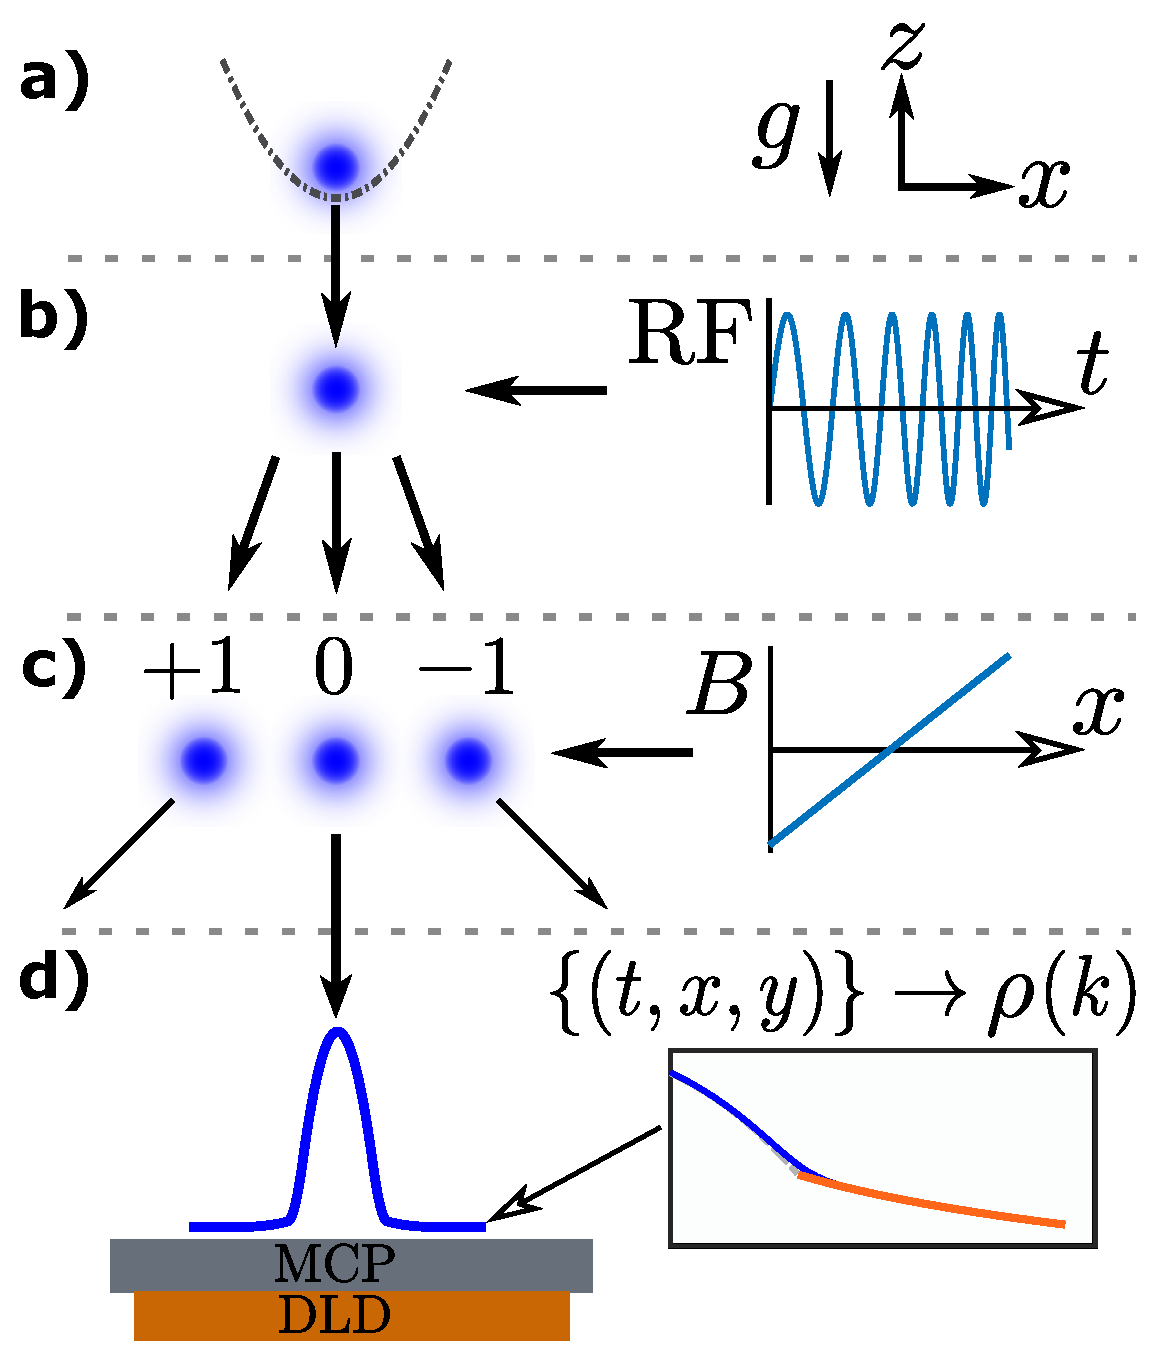
\includegraphics[width=0.4\textwidth]{fig/depletion/main/exp_cartoon}
% % 	    \caption{Sketch of experimental sequence.
% 	A BEC is released from a harmonic trap with (a) and expands during freefall before being split into a superposition of the $m_J\in\{-1,0,1\}$ states (b) by an RF chirp.
% 	A magnetic field gradient separates the clouds (c) ensuring that only the magnetically insentitive $m_J=0$ cloud lands on the detector (d), from which the momentum information is reconstructed.
% 	The quantum depletion lies in the dilute tails at large momentum (inset).}
% % 	    \label{fig:sequence}
% % 	\end{figure}

	


% % \section{Analysis} 

% % 	\begin{figure}[t]
% % 	        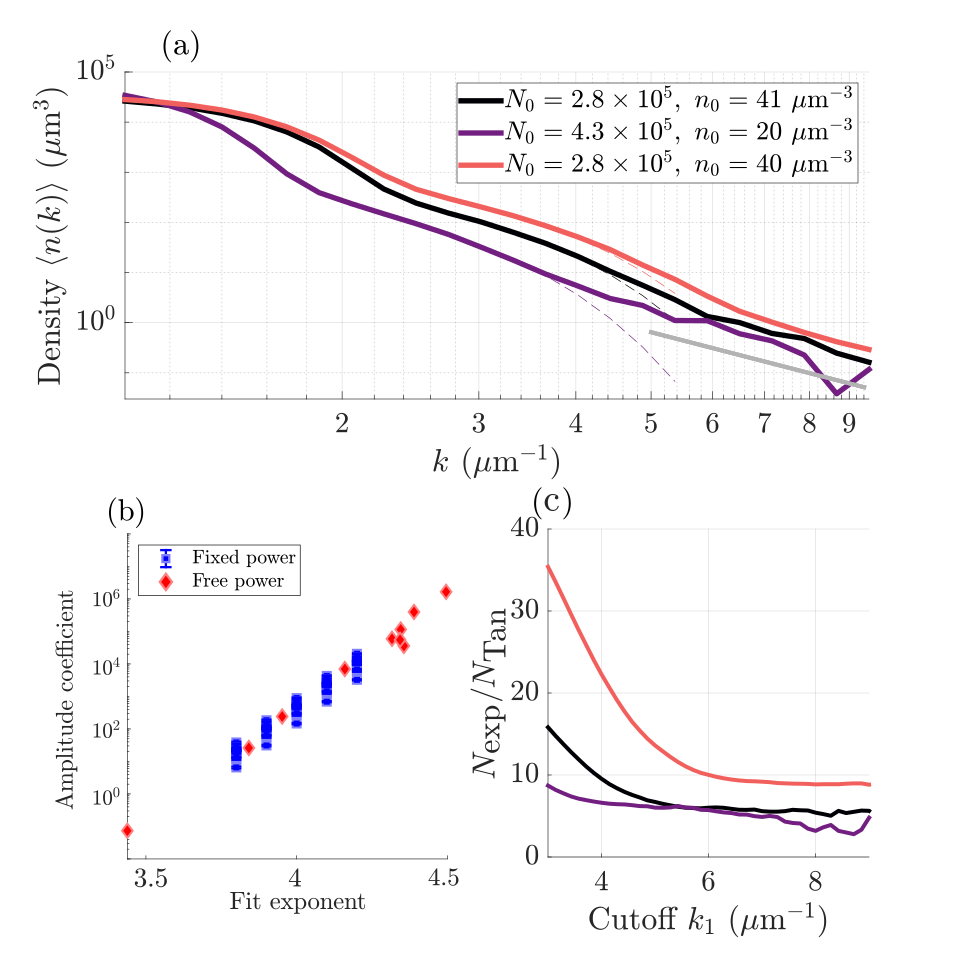
\includegraphics[width=0.5\textwidth]{fig/depletion/main/contact_determination_rev}
% % 	        \caption{The empirical density of particle momenta (a) for different peak densities, where fits to the thermal parts (dashed lines) display exponential decay, which give way to the depletion region, which decays appears to decay with $k^{-4}$ (grey dot-dashed line).
	
% % 	        In (b) we demonstrate the sensitivity of the fitting parameters to constraints in the power law.
% 	Blue squares show the amplitude coefficient $C$ given an exponent $\alpha$ fixed at five values in the range [3.8,4.2], applied to all data sets.
% 	For comparison, leaving $\alpha$ as a fit parameter gives a wide variation in best-fit exponents and scale coefficients.
% % 	        In (c) we show a way around this issue by comparing the number of atoms within the depletion region with the predictions of Eqn.
% 	(\ref{eqn:pred_num}).
% 	We fix $k_2=10\mu\textrm{m}^{-1}$ and $\phi_c=\pi/3$ to define the ROI, and show that $C_\textrm{exp}$ is not significantly dependent on $k_1$ in the depletion region $k\gtrsim6\micron^{-1}$.}
% % 	        \label{fig:cdfplot}
% % 	\end{figure}


% % 	In Fig.
% 	\ref{fig:cdfplot} (a) we show the empirical density $n(k)$ for three representative data collection runs.
% 	The three regimes of the condensate, thermal depletion, and quantum depletion span over five orders of magnitude in density.
% 	The thermal part of the distribution is well fitted by the momentum distribution of an ideal Bose gas,
% % 	\begin{equation}
% % 		n_T(k) = N_T \frac{g_{3/2}\left(\exp(-k^2 \lambda_{dB}^2/4\pi)\right)}{1.202(2\pi/\lambda_{dB})^3}
% % 		\label{eqn:th_fun}
% % 	\end{equation}
% % 	wherein the thermal de Broglie wavelength $\lambda_{dB} = \sqrt{2\pi\hbar^2/(m k_B T)}$  yields an estimate of the temperature $T$ (between 100 and 320 nK (accurate to order 10\%) in our experiments).
% 	Here, $g_{3/2}(\cdot)$ is the standard Bose integral and $N_T$ is the number of atoms in the thermal part.
% % 	The thermal population decays exponentially with $k$, as shown in Fig.
% 	\ref{fig:cdfplot} (a), and hence cannot account for the counts we observe beyond $k\gtrsim 5~\micron^{-1}$.
	
% % \subsection{Issues with analysis of power laws}	

% % 	However, fitting histograms with power-law functions is prone to biased estimates of parameters and drastic underestimation of uncertainties, especially when data is available over less than a couple of decades of dynamic range \cite{Clauset09,Virkar14}.
% 	We first demonstrate some issues with this approach, then discuss our alternative approach.
% % 	If we augment the fit function (Eqn.
% 	(\ref{eqn:th_fun})) with power-law term of the form $C/k^\alpha$, the average exponent of over all runs is 4.2(4).
	
% % 	For comparison, the prior work \cite{Chang16} reported power-law tails with an exponent 4.2(2).
% % 	At first glance, one could simply determine the amplitude of the tails by fixing the exponent to 4, and perhaps achieve better results by using a fit weighting proportional to $k^4$.
	 
% % 	However, as we argue here, there are two issues which preclude such an appealing approach.

% % 	First, in Fig.
% 	\ref{fig:cdfplot} (b) we illustrate how the exponential relationship between the scaling exponent $\alpha$ and the scale coefficient $C$, given the same data.
% % 	% hen fitting a power-law of the form $Ck^{-\alpha}$ to fixed data.
	
% % 	The coefficient $C$ varies over about three orders of magnitude as one uses different exponents $\alpha$ which lie within the range of uncertainties reported here and in the prior work \cite{Chang16}.
	
% % 	For example, fixing $\alpha=4$ in our fits (within the systematic variation) yields a fit amplitude which differs by from the best-fit value by up to a factor of order $100$.
	
% % 	Furthermore, this problem is not captured by the error estimates in the fitting routines: The error bars representing the uncertainty in fit amplitude are smaller than the markers used in Fig.
% 	\ref{fig:cdfplot} (b).
	
% % 	Finally, a linear fit shows that $d \log_{10} C/d\alpha \approx 6.8$, from which we can find the exponent that would yield an amplitude in agreement with Eqn.
% 	(\ref{eqn:pred_scaling}).
	
% % 	This turns out to be approximately 3.9, which is not distinguished with statistical significance from the results of the fitting procedures described here.
	
% % 	Conversely, we can estimate that the best-fit exponents reported in the prior work would lead to scale coefficients a factor of about 23 greater than their conclusions.
	
% % 	This demonstrates that the choice of fit exponent has an outsize influence on the estimate of the corresponding amplitude.
	
% % 	It would be easy to choose $\alpha$ which is not statistically significantly different from the best-fit estimates and arrive at a conclusion which agreed perfectly with the predictions of Eqn.
% 	(\ref{eqn:pred_scaling}), or indeed essentially any tail amplitude one wants.

% % 	Second, a deceptively reassuring result can be found by multiplying the empirical density by $k^4$, observing a flat region, and adding a constant term in an appropriately scaled model of the thermal region (i.e.
% 	Eqn.
% 	(\ref{eqn:th_fun}) multiplied by $k^4$).
	
% % 	In fact, this offers no such recourse.
% % 	Suppose the density decays as some $C k^{-(\alpha+\epsilon)}$: then the scaled density is simply $C k^{-\epsilon}$.
	
% % 	We showed above that a variation of the exponent on the order of a few per cent is both within the systematic error of the fitting procedure and also sufficient to yield drastically different conclusions.
% % 	A variation in $\alpha$ of this size would manifest as a difference of only a factor of order $2^{0.1}\approx1.07$ over the range $5\micron^{-1}\gtrsim k\lesssim10\micron^{-1}$, which is the entire region investigated both here and in the prior work.
% % 	This variation of less than $10\%$ is swamped by the noise in the individual density profiles and is not distinguishable from the run-to-run variation in the power law.

% % 	In sum, there are problems with fitting power laws and it is not clear that the conclusions drawn from such an analysis are insightful even at the best of times.
% % 	In general, determining the exponent of a power law is difficult and requires data over several orders of magnitude in scale \cite{Clauset09,Virkar14}.
% % 	\com{In this case, one could argue that there is a physical rationale for employing $\alpha=4$, but...}
% % 	The preferred statistical tools for analysing power law distributions are maximum likelihood estimators \cite{Goldstein04,Clauset09,Virkar14,Hanel17}, but these are unsuitable here because there are multiple  sources of detection events (discussed further in Appendix A).
	
% % 	Therefore it may not be possible to precisely determine the exponent of a putative power law decay for purposes of the comparison with theory.
	
% % 	We circumvent this issue by using a simpler point of comparison: the number of atoms detected within a region of interest (ROI).
% 	Moreover, we will show that the population of the tails depends on the condensate parameters in agreement with the theory of the contact, albeit up to a constant factor.
	
% % \subsection{Quantifying excess tail amplitude}

% % 	Under the null hypothesis that the \emph{in situ} depletion survives the expansion and escapes the condensate undisturbed, one can integrate Eqn.
% 	(\ref{eqn:pred_scaling}) to predict the expected number of atoms whose wavevector has a modulus in the interval $k\in (k_1, k_2)$, 

% % 	\begin{align}
% % 	\mathcal{N}_\textrm{Tan} &=\frac{\mathcal{C}}{2\pi^2}\left(\frac{1}{k_1}-\frac{1}{k_2}\right)
% % 	\label{eqn:pred_num}
% % 	\end{align}
% % 	 % The noise floor is set by the detector's dark count rate, which contributes an average of less than 1 counts to the region of interest per shot
	
% % 	The null hypothesis can be compared with the experimental results once the bounds of the ROI have been specified (namely, the values $k_1$ and $k_2$, and the solid angle of integration).
% 	We face a tradeoff in the choice of $k_2$ and the minimum elevation angle $\phi_c$ in defining the region of interest.
% 	This is because the field of view of our detector is limited by the 40mm radius of the circular detection surface to $\lesssim5\times 10^6$ m$^{-1}$ in the $(x,y)$ plane, which is only just sufficient to reach past the edge of the thermal region.
% 	The collection volume is maximized for $\phi_c=\pi/3$ rad and $k_2=10^7$ m$^{-1}$, centred on the BEC.
% 	This amounts to an ROI consisting of two vertically oriented conical sections, each with half-angle $\pi/6$, encompassing a total solid angle of $0.13\times 4\pi$ steradians.
	

	
% % 	In Fig.
% 	\ref{fig:cdfplot} (c) we compare the number of detected atoms, corrected for state transfer and detection efficiency, with the predictions obtained from Eqn.
% 	(\ref{eqn:pred_num}) as a function of the lower bound $k_1$ with $k_2=10~\micron^{-1}$ and $\phi_c=\pi/3$.
	
% % 	We consider the average of the quantity $C_\textrm{exp}=N_\textrm{exp}/N_\textrm{Tan}$ over the range $6~\micron<k<10~\micron$, outside the thermal region, as a test statistic for the null hypothesis.
% % 	The uncertainty in a single run is identified as the variance in the estimate over the ROI.
% % 	Averaging over all runs yields an average of 8(1) times as many counts as predicted by Eqn (\ref{eqn:pred_num}), where the final uncertainty is the standard error in the mean and only the most significant digit is shown.
% % 	Thus, while the observed momentum distribution appears consistent with a $k^{-4}$ asymptotic decay, the amplitude of these tails contradicts the null hypothesis of Eqn.
% 	(\ref{eqn:pred_num}) by 5.4$\sigma$.
% 	This would seem to be a count against the interpretation of these tails as a signature of the quantum depletion.
% 	However, we note two pieces of evidence that give weight to this interpretation.
	
% % 	% While at first glance this seems consistent with the fitting procedure, we find that the latter is not stable inasmuch as....	
	
% % \subsection{Consistency in effect size scaling}


% % 	First, the amplitude of the tails scales with $\bar{\omega}$ and $N_0$ in a manner consistent with Eqn.
% 	(\ref{eqn:TotalHarmonicContact}), which can be seen in Fig.
% 	\ref{fig:results_comp}, where we show the estimated contact $C_\textrm{exp}$ obtained by inverting Eqn.
% 	(\ref{eqn:pred_num}).
	
% % 	On one hand, the linear scaling of $C_\textrm{exp}$ with the product $N_0n_0$ is consistent with Eqn.
% 	(\ref{eqn:pred_scaling}).
	
% % 	In fact, this means $C_\textrm{exp}$ scales with $\left(\omega^6 N_0\right)^{1/5}$, i.e.
% 	as predicted by Eqn (\ref{eqn:TotalHarmonicContact}).
	
% % 	Indeed, if we consider the data from each trap configuration separately, the results are also consistent with the same scale factor as above.
% % 	In the absence of another known quantity which exhibits this specific nonlinear scaling relationship, we conclude this line of evidence is supportive of the tails as originating in the quantum depletion.
	
% % 	Second, we find evidence in our simulations (see next section) that the momentum-space signature of the quantum depletion does survive the condensate expansion, and indeed appears in excess of the predicted \emph{in-situ} depletion.
% 	Moreover, several features common to both experimental and simulated momentum distributions emerge, strengthening the identification of the momentum tails with the quantum depletion.
	

% % 		\com{Remarkably, if we do fix $\alpha=4$ then we find fit coefficients that are, on average, 7.8(1.7) times the predicted contact, whereas the fits with free exponents produce a wide range of coefficients, of the order of $4(8)\times10^3$ times the value of the contact calculated using Eqn.
% 	\ref{eqn:pred_scaling}, where the uncertainty is the standard deviation of the fit coefficients.

% % 		In short, it seems that fiddling with the exponent (even by only 0.2 our of 4) is not analytically justified.
% 	This might be ameliorated if there was good physical reason to assume that we are looking at a fourth-power decay, but this is motivated reasoning: In the question of whether or not this is quantum depletion, an almost-matching power law is not a smoking gun, and the sensitivity of the conclusions is remarkable.
% 	More remarkable is the fact that despite these methodological issues, in this specific instance the agreement with a more stable method should not be seen as vindication, but rather as good luck.}


% % 		 Don't seem to have the statistical strength to comment on the istortion of the profile
% % 		Second, we have similar deviation from the power-law distributed momenta in semiclassical simulations.
% 	By simulating the motion of particles with a power-law momentum distribution as they interact with an expanding parabolic mean-field potential in three dimensions, one finds increase in the weight of the momentum tails at small momentum, but the large-$k$ particles are unaffected.
% 	This causes a deviation from the power-law behaviour and a decay slightly faster than $k^{-4}$.
% 	Indeed, a note published by one of the authors of \cite{Chang16} found this effect in 1D \footnote{available via https://web.archive.org/web/20210506045825/https://github.com/rocksonchang/Helium-iPythonNotes/tree/master/20160629\%20-\%20Meanfield\%20kick} and we made similar observations in 3D semiclassical simulations.
% 	Therefore, the exponent slightly greater than 4 is not obviously inconsistent with the population arising from the quantum depletion.
% 	What is surprising is that the amplitude is so much greater than expected, and so we turn to our simulations for further insight.
	
% % 	\begin{figure}[t]
% % 	        \includegraphics[width=0.5\textwidth]{fig/depletion/main/results_comp}
% % 	        \caption{Comparison of simulations and experiments.
% 	The inset is a zoomed view.
% 	 From our empirical data (ED) we determine the empirical contact $C_\textrm{exp}$ which is linear in the product $N_0n_0$ (as predicted by Eqn.
% 	(\ref{eqn:pred_scaling})), but 8(1) times more sensitive (Av) than the prediction by the Tan theory (TT).
% 	The simulated contact of BECs in a cigar-shaped trap (CT) are consistent with (TT) before release and increases after expansion (CE), but by less than the experiment.
% 	A slow relaxation of the tight axes of the cigar trap (CS) leads to a reduction in the simulated contact.
% 	Simulations of a spherical trap (ST) show a negligible increase after expansion (SE).
% 	The prior \mhe result \cite{Chang16} (IO) is shown for comparison (dashed line)}
% % 	        \label{fig:results_comp}
% % 	\end{figure}

% % \subsection{Experimental details}

% % \subsubsection{Trap configuration and calibration}

% % 	We prepared our BECs with via forced evaporative cooling in a harmonic magnetic trap with trap frequencies $(45,425,425)$ Hz and a DC bias stabilized by our auxiliary field compensation coils \cite{Dall07,Dedman07}.
% 	For the tight trap we increased the coil current after the cooling sequence to obtain trapping frequencies $(71,902,895)$ Hz, ramping the field as a sigmoid step function to minimize in-trap oscillations.
% 	Note that the weak ($x$) axis of the trap is horizontal, with tight vertical confinement.
% 	The trap remained on for 150ms before switching the trap off with a $1/e$ time of $\approx38\mu$s.
% 	The condensates were allowed to expand for 2ms before we transferred some of the condensate into the magnetically insensitive $m_J=0$ state via Landau-Zener sweep to prevent distortion by stray magnetic fields.
% 	The RF pulse was created by a  function generator, amplified, and applied to the experiment chamber by a coiled antenna inserted into the BiQUIC coil housing.
% 	The pulse swept from 1.6-2.6MHz over 1ms and was centred on the fine structure resonance between the $m_J$ states.
% 	The transfer efficiencies $\eta_j$ for each of the $m_J = j$ states is discussed in the next section.
% 	The sweep was $10^6$-fold wider than the Doppler broadening of the BEC which ensured uniform transfer at all momenta.
% 	Immediately after the RF sweep, the bias coils are switched off and auxiliary push coils in the vertical (Z) and weak horizontal (X) axes are activated using a fast MOSFET switch to implement a Stern-Gerlach separation of the $m_J = -1,~0,$ and $+1$ pulses.

% % 	We use a Roentdek DLD80 multichannel plate and delay-line detector stack \cite{Manning10} located 859mm below the trap, which registers the arrival times and positions $(t_i,x_i,y_i)$ of each atom, indexed by $i$.
	
% % 	The velocity of each atom relative to the centre of mass of the cloud is calculated by $(v_x,v_y,v_z) = t_{i}^{-1}(x_i-\bar{x},y_i-\bar{y},g_0(\tau^2-t_{i}^{2}))$, where $g_0$ is the local gravitational acceleration and the overbar denotes the within-shot average and $\tau=417$ ms is the time of flight of the centre of mass.
	
% % 	The far-field momentum is thus obtained via $m\textbf{v} = \hbar\kvec$.
% % 	The velocity conversion assumes a point source but carries a negligible error of a few ppm as the in-trap BEC size is smaller than the detector resolution.
	
% % 	The space and time resolution of the detector are 100 $\mu$m and 3 $\mu$s, respectively \cite{Henson18}, and the detector efficiency of $8(2)\%$ was determined from the collection efficiency of correlated atoms on the opposite sides of scattering halos \cite{shin19,shin20,Jaskula10}.
	

% % \subsubsection{Determining transfer efficiency}

% % 	To calibrate the transfer efficiencies, we applied a weaker Stern-Gerlach than for the depletion measurement, resolving each $m_J$ cloud on the detector, as illustrated in Fig.
% 	\ref{fig:frac_cal}.
	

% % \begin{figure*}[!t]
% % 	\begin{center}
% % 		\includegraphics[width=\textwidth]{fig/depletion/main/frac_cal_profile}
% % 		\caption{Determining the RF transfer efficiency.
% 	The time-of-flight profiles of each pulse are resolved (a) by applying a weak Stern-Gerlach pulse during the time of flight.
% 	The pulses are aligned with respect their centre-of-mass (b) and used to determine the pointwise fraction ((c), dotted line).
% 	Detector saturation is evident in the peaks (dashed lines), but not in the thermal tails (solid lines), which are used to compute the transfer efficiency.
% 	Because of its lower flux, the $m_J=-1$ pulse does not show evidence of saturation (d) and is used to determine the thermal fraction.}
% % 		\label{fig:frac_cal}
% % 	\end{center}
% % 	\end{figure*}

% % 	The efficiencies $\eta_J$ cannot be calculated by counting the atoms in each cloud because the detector saturates during the peak condensate flux, but we can compare the thermal parts.
% 	We align each cloud along the time (Z) axis and compute the pointwise fraction of the atomic flux $\phi(t)$ accounted for by each cloud, $\eta_j(t) = \phi_j(t)/\sum_j\phi_j(t)$, as depicted in Fig.
% 	\ref{fig:frac_cal}.
% 	The ratio of densities between the clouds is roughly constant in the thermal part, indicating the absence of important saturation effects and a spin transfer that is independent of $k$.
% 	The fraction of the original cloud transferred into each $m_J$ state is determined by taking the average $\langle\eta_j(t)\rangle$ over the thermal tails.
% 	We find these efficiencies are approximately 74\%, 24\%, and 2\% in all runs for the $m_J=+1$, 0, and -1 states, respectively.
	
% % 	While the $m_J=0$ and $m_J=1$ clouds clearly saturate the detector, the small fraction ($\approx2\%$) of the atoms transferred to the $m_J=-1$ state does not (Fig.
% 	\ref{fig:frac_cal} (d)).
% 	A bimodal fit to the condensed and thermal parts, plus constant background, yields an estimate of the thermal and condensed fractions.
	


% % % \subsection{Determination of thermal fraction}
	

% % % 	\begin{figure}[!h]
% % % 	\begin{center}
% % % 		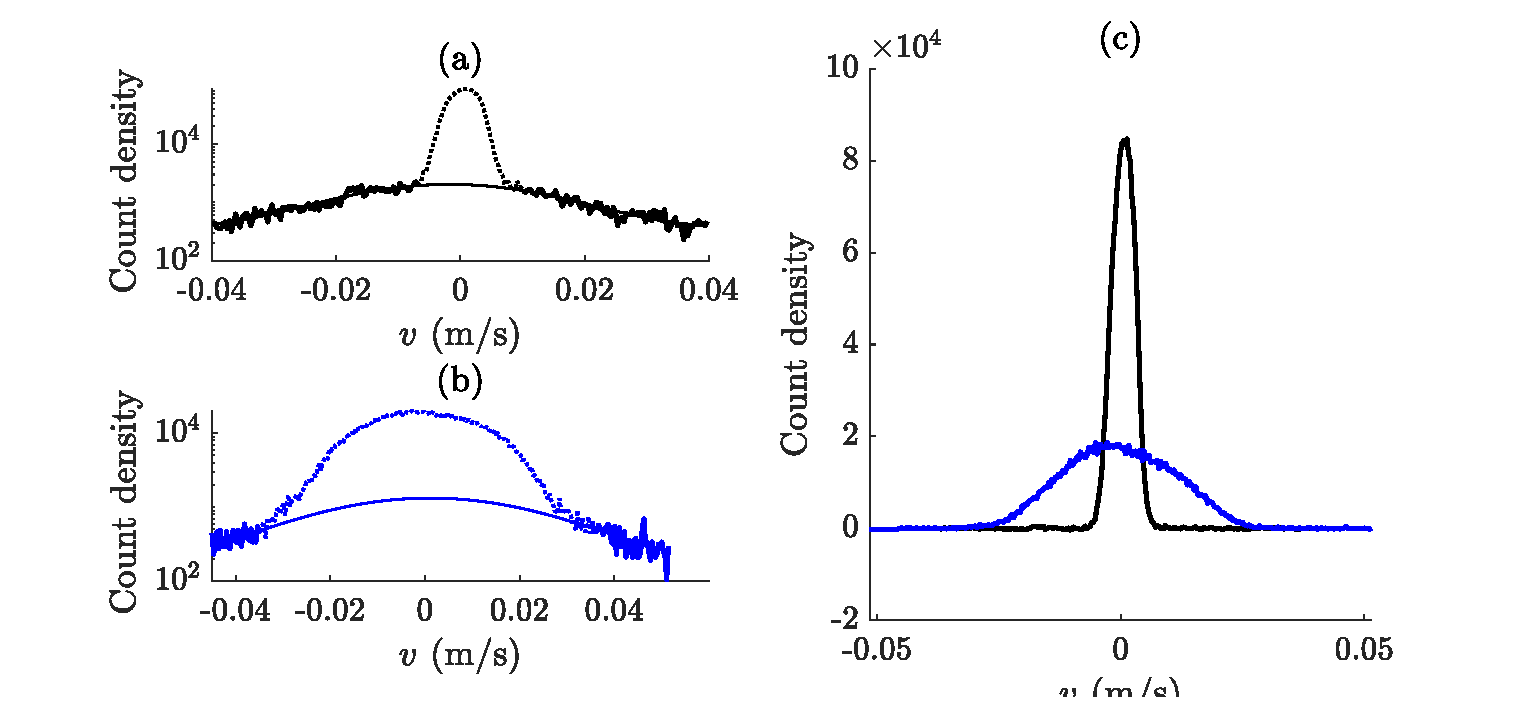
\includegraphics[width=0.8\textwidth]{fig/depletion/main/m1_frac_anal}
% % % 		\caption{Comparison of thermal fits in the unsaturated $m_J=-1$ pulse including 138 shots.
% 	The weak (X) and strong horizontal (Y) trapping axes are shown in (a) and (b), respectively.
% 	\org{would be helpful to label $v_x$ and $v_y$ to make it self-evident at 1st glance.} Both projections display a bimodal peak, with the condensate (dotted lines) and thermal parts (thick solid lines) easily distinguished.
% 	Fitting a Gaussian profile (thin solid line) to the velocity distribution of the thermal part yields the thermal number and temperature.
% 	Subtracting the fit leaves the condensate profile (c) which can be \blu{\dots something\dots} yields the condensed number.}
% % % 		\label{fig:thermal_frac}
% % % 	\end{center}
% % % 	\end{figure}



% % \subsubsection{Analysis of spin transfer measurements}

% % 	In early tests of our measurement sequence we noticed a contamination of the signal by spurious counts.
% 	We inferred these were remnant counts from the $m_J=+1$ cloud as they were still visible when we ran an experimental sequence without the Landau-Zener transfer.
% 	This contamination appeared in a particular region of our detection image, illustrated in Fig.
% 	\ref{fig:spinpop}.
% 	As such we were able to correct for it by subtracting their contribution from the counts collected during measurement shots.
% 	Generally, fewer atoms can be attributed to this noise ($\leq~1$ atom per shot, on average) than would be required to explain the discrepancy described in the main text ($5-10$ counts per shot).
% 	While the cause of the cross-contamination is unclear, we observe that the count density outside the region of interest is similar in both the shots with the RF pulse and those without.
% 	We hypothesize that the remnant counts are atoms transferred into the $m_J=0$ state by non-ideal behaviour of the Stern-Gerlach pulses.
% 	We note that only about one in a million atoms from the $m_J=1$ cloud present in this manner in a given shot.

% % 	As mentioned in the main text, the presence of these counts also prevents a straightforward application of a maximum-likelihood estimator (MLE) to determine parameters of the power-law region.
% 	The basic principle of the MLE is to assume a functional form for the probability distribution $p(x|\theta)$ underlying the observed data $x$, and dependent on some parameters $\theta$; the zero of the derivative of the \emph{likelihood} function $L(\theta|x)$ with respect to the parameters $\theta$ then yields the most-probable parameter values given a set of observations $x$.
% 	In our context, one can assume a functional form for the probability distribution underlying atomic detection events (via a wavefunction ansatz).
% 	The detector dark count rates can also be incorporated by assuming a uniform distribution, although this necessitates a cumbersome procedure to retain proper normalization.
% 	Such an analytical treatment does not readily permit the inclusion of an empirical density estimate which itself includes the aforementioned dark count rate.
% 	Instead, we opt for the simpler approach described in the main text.

% %     \begin{figure}[!b]
% % 	\begin{center}
% % 		\includegraphics[width=\columnwidth]{fig/depletion/main/spinpop}
% % 		\caption{Measured contribution of the detector dark counts and spurious spin counts to the time-of-flight profile.
% 	We accounted for the pulse at around 550ms and subtracted it from the measured profiles when computing the contact.
% 	After removing this background term, the density profiles above and below the condensate agree, indicating convergence on the true signal.
% 	For reference, the peak flux of the $m_J=0$ condensate is about a thousandfold greater than the peak shown here.}
% % 		\label{fig:spinpop}
% % 	\end{center}
% % 	\end{figure}

% % 	% \begin{figure}[!h]
% % 	% \begin{center}
% % 	% 	\includegraphics[width=\textwidth]{fig/depletion/main/profile_overlay}
% % 	% 	\caption{Comparison of average time-of-flight profiles over a single data run for the quantum depletion measurement shots (blue, 871 shots), transfer efficiency calibration (black, 112 shots), detector dark counts (red, 871 shots), and spurious counts (dot-dash, 895 shots).
% 	The time window bounded by $|k|\leq 10\mu$m is indicated with dotted lines.
% 	Shaded area is the standard error over the entire run.}
% % 	% 	\label{fig:tof_profile}
% % 	% \end{center}
% % 	% \end{figure}




% % % Note that the temps disagree between axes, but within axes between clouds they are consistent(....ish).
% 	This means we can use the profile ratio method, which is also consistent with comparing the thermal number from the fits.
% % % Perhaps comment on the thermal-subtracted part; the TF profile should have a sharp cutoff, but the smooth edges are suggestive evidence of this roll-off

% % % \begin{figure}
% % % 	\centering
% % % 	\includegraphics[width=0.5\textwidth]{fig/depletion/main/counts_per_run}
% % % 	\caption{Number of counts detected in the region of interest in the depletion measurement (a), the spin mixing calibration (b), and the dark count calibration (c).
% 	An average of 3.0(5) counts were detected in the ROI in the spin-mixing calibration shot, and the background count rate was 0.4(2) counts per shot.
% 	Separate lines indicate separate \emph{runs}, i.e.
% 	sequences of shots with fixed parameters.}
% % % 	\label{fig:num_counts}
% % % \end{figure}


% % \subsection{Peak density calibration}

% %     The quantum depletion and contact are both predicted to depend solely on the condensed number and trapping frequencies via the condensate density, hence it is important to determine both quantities accurately.
% 	In the Thomas-Fermi approximation, the peak density of the condensate can be written as $n_0 = \mu/g$, where $\mu$ is the chemical potential, $g=4\pi\hbar^2a_{1,1}/m$ is the effective interaction strength, $m\approx6.6\times10^{-27}$ kg is the atomic mass, and $a=7.512$ nm is the s-wave scattering length between pairs of atoms in the $m_J=1$ state \cite{Moal06}.
% 	The sole experimental parameters in the expression for the peak density (Eqn.
% 	\ref{eqn:n0}) are $\bar{\omega} = \left(\omega_x\cdot\omega_y\cdot\omega_z\right)^{1/3}$,  the geometric trap frequency, and $N_0$, the number of atoms in the condensate.
% 	During these calibration runs we simultaneously determine the total atom number $N$ and trap frequency $\bar{\omega}$ in a single shot using a pulsed atom laser and use the thermal fraction (as below) to determine the condensed number $N_0$.
	

% % 	The pulsed atom laser consists of a series of Fourier-broadened RF pulses centred on the minimum Zeeman splitting in the trap.
% 	The pulse transfers atoms in the trap to the untrapped $m_J=0$ state with an approximately constant transfer rate across the cloud.
% 	We outcouple approximately 2\% of the atoms per 100$\mu$s pulse for $\approx$200 pulses, which eventually depletes the entire trap.
% 	The atom laser thus prevents the detector from saturating and allows an accurate determination of the atom number, up to a factor of the quantum efficiency.
% 	We determine the trapping frequencies by inducing centre-of-mass oscillations with a magnetic impulse, and finding the oscillation period from the atom laser pulses \cite{henson18ML}.



% % \section{Numerical simulations}
% % \label{STAB}

% % 	We performed simulations of the BEC expansion from harmonic traps using the first principles STAB method \cite{Deuar11,Kheruntsyan12}.
% 	The simulations included a cigar-shaped trap (marked CT in Fig.
% 	\ref{fig:results_comp}) with parameters matched to the experimental conditions.
% 	The in-trap state was consistent with the adiabatic sweep theorem before release from the trap.
% 	Following expansion from the cigar trap (CE in Fig.
% 	\ref{fig:results_comp})), the simulated tail amplitude increased and stabilized within a few hundred microseconds, much sooner than the 2ms delay between the trap release and application of the rf and Stern-Gerlach pulses.
% 	Fig.
% 	\ref{fig:time_dep_theory} shows time evolution of the tail amplitude for the simulated traps using the same ROI as the experimental setup.
% 	 In this configuration the steady-state value of the momentum tails was a factor of 1.64(9) above the predictions of Eqn.
% 	(\ref{eqn:pred_scaling}).
	

% % 	To understand the disagreement with earlier theory \cite{Qu16}, which predicted no depletion survival, we also investigated the effect of adiabatic expansion on the in-trap depletion by simulating a slow decrease of the transverse trapping frequencies by a factor of two (CS), and found that the in-trap contact decreased roughly as predicted by Eqn.
% 	(\ref{eqn:pred_scaling}) in these instances --- see the dashed line in Fig.~\ref{fig:time_dep_theory}.
	

% % 	We also found that the factor of disagreement (i.e.
% 	$C_\textrm{sim}/C_\textrm{Tan}$) between Eqn.
% 	(\ref{eqn:pred_num}) and the simulated tails depends on the angle choice of cutoff angle $\phi_c$.
% 	Put another way, the momentum distribution in the simulations is anisotropic and takes the form $f(\theta,\phi)/k^4$.
% 	We note that the average of an angle-dependent power law decay over a region $\Omega$ is simply $\langle f(\theta,\phi)\rangle_\Omega/k^4$, preserving the power-law behaviour.
% 	We find a similar effect in the experimental data as well, albeit with low statistical significance owing to the small signal-to-noise.
% % 	Specifically, we find that $C_\textrm{exp}$ is larger for smaller collection regions that are more tightly concentrated about the vertical (strong) trapping axis, whereas larger collection angles (including areas closer to the weak axis) produce a lower $C_\textrm{exp}$.
% % 	We quantify this effect in Tab.
% 	\ref{tab:angle_dep} and propose physical origins of our observations in the next section.
	

% % 	\begin{figure}[t]
% % 	        \includegraphics[width=0.5\textwidth]{fig/depletion/main/time_dep_theory}
% % 	        \caption{Simulations of condensates released from a cigar-shaped trap show an increase in contact after the trap release, stabilizing after a time on the order of $1/\omega_x$, several hundred $\mu$s.
% 	The relative difference between in-trap and expanded contact increases with the density of the condensate.
% 	For comparison, the experimental control pulses are implemented after 2ms of expansion.
% 	In contrast, when the transverse trapping frequencies are reduced by half (dotted line), the in-situ contact relaxes.}
% % 	        \label{fig:time_dep_theory}
% % 	\end{figure}

% % 	\begin{table}[b]
% % 		\begin{tabular}{c c c}
% % 			\hline\hline
% % 			Half-angle &	$C_\textrm{exp}/C_\textrm{Tan}$ &	$C_\textrm{sim}/C_\textrm{Tan}$\\
% % 			\hline
% % 			10	&	9.3(3.3) &	2.2(3)\\
% % 			20 	&	8.7(1.8) &	1.9(2)\\
% % 			30	&	8.0(1.3) &	1.6(1)\\
% % 			\hline\hline
% % 		\end{tabular}
% % 		\caption{The excess of detection events over the expected number depends on the choice of angular bounds for the ROI.
% 	We show the average factor of disagreement between experimental and predicted counts for three half-angles defining the two vertically oriented conical sections.
% 	For comparison, we show the factor of disagreement for the $C_\textrm{sim}/C_\textrm{Tan}$simulated case where $n_0=44~\micron^{-3}$.}
% % 		\label{tab:angle_dep}
% % 	\end{table}

% % % \include{sim_part}


% % \section{Discussion}

% % 	We interpret these results as an indication that the depleted atoms are accelerated by the non-uniform mean-field energy of the condensate during the expansion.
% % 	In detail, after a quench into the free particle regime, the condensate expands hydrodynamically on timescales of $1/\omega$.
	
% % 	This is an adiabatic process for the low momentum depletion, whereby some depleted atoms are absorbed back into the condensate in agreement with \cite{Qu16}.
% % 	However, the characteristic time for reabsorption is $\hbar/gn_0$, slow enough that quasiparticles in the particle branch of the Bogoliubov dispersion have sufficient velocity to escape the expanding cloud without being reabsorbed and thus transition to free atoms.
	
% % 	This effect contributes to the disagreement between \emph{in situ} and measured tail amplitudes, hence $C_\textrm{exp}$.

% % 	Moreover, an atom inside the BEC experiences an effective force from the gradient of the mean-field potential $\textbf{F} = -4\pi\hbar^2a \nabla  n(x)/m$.
	
% % 	This endows escaping depleted particles with a greater momentum, increasing the weight of the tails in the far-field.
	
% % 	This effect is exacerbate in light atoms like $^{4}$He: because the acceleration scales with $1/m^2$, it would be suppressed by a $\sim500$-fold in $^{87}$Rb experiments \cite{Makotyn14}.
	
% % 	Further, it is much easier for depletion atoms to escape and be accelerated in the transverse x-y directions from an elongated cloud because the distances $R_{TF}=\frac{1}{\omega}\sqrt{2gn_0/m}$ are reduced by $\bar{\omega}/\omega_{x,y}$, whereas the initial mean depletion velocities \textit{in situ} $v\sim \sqrt{2gn_0/m}$ are isotropic.
% % 	Indeed, spherical clouds (SE) exhibit a much weaker effect than the elongated clouds (CE) owing to the longer escape time.
% % 	Furthermore, we find some evidence that this anisotropic feature is present in our experimental data.
	
% % 	The hypothesis that this conjunction underlies the observed effects is further supported by our simulations: We observe a decrease in the total number of depleted particles (reabsorption) and a simultaneous increase of the large-k population (forcing).
	
% % 	This constitutes a partial explanation of the experimenal findings too, exhibiting important similar features including the anisotropic distribution and nonlinear scaling consistent with the quantum depletion.
	

% % 	\com{Two factors to address: Detector efficiency and the Landau-Zener transfer}


% % 	However, a mystery remains: Why is the excess depletion some four times greater than accounted for by this picture? This issue should be resolved in order to interpret far-field observations in terms of the in-trap physics of interest.
	
% % 	This question invites complementary studies of the \emph{in situ} depletion in \mhe BECs.
	
% % 	The cause of the contact anomaly could be elucidated by determining whether it originates in the trapped condensate, or is generated during the trap release and expansion.
	
% % 	Such an investigation requires an \emph{in situ} probe of the contact, such as RF spectroscopy or Bragg spectroscopy.
% % 	The latter may be the most fruitful of the two simply because of the difficulty of interpreting the results from the former, which we sketch here.
	
	
% % 	The basic principle of RF contact spectroscopy is to apply a monochromatic RF probe which is detuned from the resonance between two spin states, coupling atoms in the initial spin state to an untrapped channel.
	
% % 	One then performs a differential measurement of the atom number and expects the signal strength to scale as $\omega_\textrm{RF}^{3/2}$ with the detuning from the RF resonance.
% % 	The loss rate is also proportional to the difference of reciprocal scattering lengths $\Gamma\propto(1/a_\textrm{i,i}-1/a_\textrm{i,f})$ between pairs of atoms in initial-initial ($a_{i,i}$) and initial-final ($a_{i,f}$) spin states \cite{Braaten10,Wild12}.
	
% % 	For He$^*$ (spin 1) the scattering lengths $a_{1,1}$ and $a_{1,0}$ are identical \cite{Leo01}, rendering the preferred $m_J=1-m_J=0$ transition unusable.
	
% % 	On the other hand, $a_{1,-1} = 3/7 a_{1,1}$ \cite{Vassen16}, and the singlet transition can be driven without populating the $m_J=0$ state.
	
% % 	In principle this could produce a detectable flux of atoms to perform sensitive in-trap contact measurements, however, collisions in the $^1\Sigma_{g}^{+}$ channel have large Penning ionization rates which lead to significant trap losses \cite{Leo01}.
	
% % 	The ionization products would be detectable by in-vacuum channel electron multipliers but require theoretical work to disentangle from the spectroscopic signal.
	
% % 	Further, while other atomic species offer Feshbach resonances by which to tune the inter-species scattering length (and hence signal or ionization rate), \mhe has no such feature.
	
% % 	While such a measurement is not \emph{prima facie} impossible, Bragg spectroscopy may yield more readily comprehensible results.

	
% % 	\section{Conclusion} 

% % 	Our work expands the growing suite of far-field investigations of quantum depletion \cite{Cayla20,Chang16} and confirms that quantum depletion can, remarkably, survive past the lifetime of its original condensate.
% 	Our findings clarify that how the depletion can be visible in the far-field momentum distribution here and in earlier experiments, and that the hydrodynamic approximation does not capture sufficient short-wavelength information to make detailed predictions about the high-momentum behaviour.
% 	We thus find a partial explanation for the deviation of the far-field distribution from both the predicted in-situ depletion and the hydrodynamic reabsorption: The interplay between coherent absorption of Bogoliubov excitations and the dispersal of the chemical potential into kinetic energy, to which helium is particularly sensitive, result in a growth of the $k^{-4}$ tails of the momentum distribution during freefall.
% 	It would be informative to determine whether this discrepancy originates in the trapped condensate or is due to some unknown non-equilibrium effect during expansion.


% % 	\section{Acknowledgements} We Would like to thank David Clement, Raphael Lopes, Jean Dalibard, and Karen Kherunstyan for their helpful discussions.
% 	This work was supported by Australian Research Council (ARC) Discovery Project Grants No.
% 	DP160102337 and No.
% 	DP190103021.
% 	S.
% 	S.
% 	H was supported by DECRA DE150100315,  J.A.R., D.
% 	K.
% 	S.
% 	by the Australian Postgraduate Award (APA), and K.F.T.
% 	by the Australian Government Research Training Program (RTP) Scholarship.
% 	The simulations by P.
% 	D.
% 	were supported by National Science Centre (Poland) grants No.
% 	2018/31/B/ST2/01871 and 2012/07/E/ST2/01389.

% % \nocite{Manning10,Henson18,shin19,shin20,Jaskula10,Dall07,Dedman07,Moal06,henson18ML,PethickSmith,braaten10,wild12,Leo01,vassen16,Deuar11,Kheruntsyan12,Drummond80,Deuar07,Sinatra00,Kheruntsyan12,Deuar11,Krachmalnicoff10,Lewis-Swan14,Lewis-Swan15,Deuar13,Deuar14,nstab-longpaper,Drummond80,Deuar11,tcorr,Deuar13,FINESS-Book-Ruostekoski,FINESS-Book-Sinatra,Martin10a,Martin10b,Sinatra02,Norrie06,Deuar11,DeuarPhD,Drummond20,stob,nstab-longpaper}

% % \bibliography{bibliography}
% % \appendix
% % %\section*{Supplementary Materials}

%\comment{sections just dumped from main text for now - clean up later}



%Our bespoke software interfaces with the LabView control environment and loops over a sequence of experiments, consisting in this case of: Atom number calibration, Trap frequency calibration, and RF transfer efficiency, followed by 10 data collection runs.

%To calibrate the atom number, we used an RF pulse sequence to create a pulsed atom laser with intensity well below the saturation threshold of our delay-line detector. We corrected the number of detected atoms to account for the quantum efficiency ($\sim$8\%) of our detector. 
%\comment{Should use QD measurements to compute condensate/thermal fraction relative sizes and further improve $N_0$ measurement}.
%\comment{how does this compare to our trap binning? What is the uncertainty of the QE?}

%Together with the atom number, a measurement of the centre-of-mass motional frequencies allowed us to compute the peak density of the condensate. We measured the trap frequency by transient magnetic field to the trapped condensate for $\sim 150\mu s$, forcing centre-of-mass motion in the lab frame. We used the same pulsed outcoupling scheme as in the number measurement, and measured the  centre-of-mass momentum of the cloud at the time of each pulse. Our outcoupling frequency is well below the natural frequency of the confining potential so we used a subsampled reconstruction method to recover the trap frequency. Prior to running experiments we varied the outcoupling pulse frequency to determine in which Nyquist zone the actual trap frequency lies relative to our sampling frequency. We can then obtain the trap frequency to within precision X in a single shot of the experiment by taking a Fourier transform of the centre of mass motion.

%Our calibration sequence provided accurate number and peak density measurements along with the condensate profile. We verified the spherical symmetry of the thermal and depleted fractions, and so compute the momentum density by an average over a large section of the momentum distribution. 

%We verified the fitting method by analysing a test data set of known parameters, which was generated by the Metropolis-Hastings algorithm, and find the method recovers the test set parameters within a factor less than our experimental uncertainties.  


%There may still be errors in the analysis. The fitting procedure apparently produces a good fit, but it may be possible to get indistinguishable or better fits by fixing the exponent of the power law to be some $\alpha\neq 4$. This would challenge the assertion that the cause of the observed profile is in fact quantum depletion.  Assuming the observed data does follow a power law, statistical fluctuations in the high-momentum region become amplified by the $k^4$ scaling procedure and could introduce further error in the estimated Tan constant. \comment{Y-error bars are computed in a fairly ad-hoc way, so ours and Chang may be drastically under-reported...)}Reliably estimating the parameters of a power-law distribution is nontrivial\cite{Clauset2009}, and the robustness of the fitting method above has not been exhaustively tested. The LDA prediction is essentially that the single-particle wavefunctions, hence the single-particle probability distribution over momentum, are affected by many-body effects. One computes the single-particle probability density by dividing the condensate density by the number of particles (hence the $N_0$ term in the LDA), and then the problem of extracting the contact parameter from the data is an exercise in statistical parameter estimation. As shown by Clauset et al \cite{Clauset2009}, fitting these functions tends to produce incorrect estimates of parameters. The method outlined in Clauset was proven to asymptotically converge with probability 1 to the correct fit parameters of a power law distribution, but would need to be extended to derive a maximum likelihood estimator for a power law overlaid on a constant background.


% % \end{document}


% % \begin{abstract}

% % Measurements of Tan's contact in expanding condensate conflict with predictions of the \emph{in situ} quantum depletion.
% 	It is unclear how the depletion survives without a condensate, and even appears stronger in the far-field than before the trap release.
% 	We confirm experimental observations of a power-law decay in the far-field, consistent with the survival of the quantum depletion.
% 	Simulations of our experiment support this conclusion and provide a partial explanation.
% 	A gap between the numerical and empirical results is an open question obstructing studies of quantum depletion in the far field.
% % % max 600chars for PRL
% % % \end{abstract}

% % % \maketitle

% % % \section{Introduction} 
% % A profusion of work on quantum degenerate matter is motivated by the promise of the prototypical coherent phenomenon, superfluidity.
% 	The underlying mechanism of superfluid formation is the Bose-Einstein condensation of collective excitations, which was realized by Bogoliubov \cite{Bogolubov47}.
% 	This finding is of broader importance because the BEC and BCS regimes of supercondictivty are characterized by condensation of molecular dimers and of Cooper pairs, respectively.
	

% % Bogoliubov formulated the problem of a homogeneous system of interacting bosons in terms of a free Bose gas of collective excitations, constituted by pairs of particles with opposite momenta \cite{vogels02}.
% 	The thermal population of quasiparticle modes produces the normal component of a superfluid, while the zero-point population, called the \emph{quantum depletion}, accounts for the large-momentum part of the wavefunction.
% 	The Bogoliubov spectrum exhibits a crossover from wavelike phonon modes to single-particle excitations at momenta larger than the speed of sound in the condensate \cite{steinhauer03}, but this description breaks down in strongly interacting systems \cite{lopes17_quasiparticle} whereas the Tan relations remain valid in the strongly-correlated regime.

% % In a modern addition to the theories of quantum matter, Tan explained how s-wave contact interactions modify the short-range pair correlation function and manifests as a power-law decay in the momentum density \cite{tan08_energetics,tan08_momentum,tan08_virial}.
% 	The contact underpins several universal relations between many-body features and microscopic information in aribitrary spin mixures at any density, temperature, and geometry \cite{combescot09,braaten08,braaten11,werner12_boson,werner12_fermion}.
% 	Emerging evidence for analogous relations in p-wave scattering \cite{luciuk16} and three-body interactions \cite{fletcher17} hints at the prospect of new systematic ways to design thermodynamic features by tailoring the interactions between particles.
	

% % Two defining properties of Tan's contact, known as the adiabatic sweep theorem \cite{tan08_momentum} and generalized virial theorem \cite{tan08_virial}, have been decisively verified via radio spectroscopy \cite{baym07,punk07,braaten10} of degenerate Bose \cite{wild12} and Fermi gases \cite{stewart10,sagi12}.
% 	Bragg spectroscopy has revealed the universality of scaling relations for the pair correlation function \cite{kuhnle10} and the behaviour of the contact across the superfluid phase transition \cite{kuhnle11,mukherjee19,carcy19}, yielding benchmarks for descriptions of strongly-correlated gases \cite{rakhimov20}.

% % The Bogoliubov theory has also yielded accurate predictions of the quasiparticle spectrum \cite{lopes17_quasiparticle,vogels02} and of the depleted population in ultracold atomic Bose-Einstein condensates \cite{xu06,lopes17_depletion} and exciton-polariton condensates in solid substrates \cite{pieczarka20}.
% 	The Bogoliubov spectrum exhibits a crossover from wavelike phonon modes to single-particle excitations at momenta larger than the speed of sound in the condensate \cite{steinhauer03}, but this description breaks down in strongly interacting systems \cite{lopes17_quasiparticle}.
% 	However, detailed study of the quantum-depleted tails of the momentum distribution has been challenging to date because the tails are beneath the noise floor of optical imaging techniques.
% 	A previous experiment sought to use a Feshbach resonance to produce a visible depleted fraction \cite{makotyn14}, but found that the momentum distribution saturated during expansion and did not display a power-law tail.
% 	This was because many-body effects shielded condensed atoms from excitation into the normal component \cite{kira15_hyperbolic,kira15_coherent}.


% % In contrast, another experiment found unexpectedly large momentum tails in the far-field of a Helium BEC released from a harmonic optical trap \cite{chang16}.
% 	This is particularly surprising because conventional wisdom argues that the density decreases adiabatically during expansion \cite{xu06}, justifying treatment with a hydrodynamic approximation wherein the tails are predicted to vanish \cite{qu16}.
% 	Instead, the study \cite{chang16} found momentum tails far stronger even than expected in the cloud before release.
% 	This contradiction implies that either helium condensates violate the minimal assumptions of Tan's theory of the contact \cite{tan08_energetics,tan08_momentum,tan08_virial}, or that far-field momentum measurements are not a straightforward means of examining the quantum depletion even in weakly interacting gases.
% 	It is important to verify and overcome this obstacle, as such measurement could play a central role in studying the microscopic physics of superfluids with ultracold gases.

% % To this end, we revisit the measurement of the momentum distribution of a helium condensate expanding from a harmonic trap.
% 	We conducted experiments using an independent apparatus and analysis, covering a range of densities twice as large as in the prior work \cite{chang16}.
% 	We observe power-law tails in the far field whose amplitude significantly exceeds the predictions of the \emph{in situ} depletion, corroborating the prior work.
% 	Our measurements are complemented by simulations of the time-dependence of the momentum distribution using a stochastic Time-Adaptive Bogoliubov (STAB) method in the positive-P framework \cite{Deuar11,Kheruntsyan12,SOM}.
% 	These show that the non-adiabatic release of the trap is responsible for survival of the depletion, and that the depleted particles acquire additional kinetic energy from the mean-field energy of the condensate during the subsequent adiabatic expansion.
% 	These factors result in an amplification of the momentum tails relative to the \emph{in situ} values and are not captured in the hydrodynamic approximation.
% 	However, quantitative disagreement between our simulations and experimental data rule out the release energy as a complete explanation for the observed excess counts.
% 	We conclude by suggesting an informative complementary approach.
	

% % \section{Experiment} Our experimental sequence, depicted schematically in Fig.
% 	\ref{fig:sequence}, began with BECs with between $2\times 10^5$ and $5\times 10^5$ $^4$He atoms polarized in the $\metastable(m_J=1)$ state and cooled to $\sim$ 300 nK by forced evaporative cooling in a harmonic magnetic trap generated by field coils in a Bi-planar Quadrupole Ioffe configuration \cite{Dall07}.
% 	The metastable $\metastable$ state, denoted He$^*$, which is 19.8eV above the true ground state \cite{Hodgman09}, enables single-particle detection in the far-field regime and thus affords direct access to microscopic momentum information.
% 	The use of a multichannel electron multiplier in combination with a delay-line detector (MCP-DLD)  \cite{Manning10} has permitted the observation of many-body momentum correlations \cite{Hodgman11,Dall13} and Hanbury Brown-Twiss bunching of both condensed \cite{Schellekens05,Jeltes07,Manning10,Dall11} and quantum depleted atoms \cite{cayla20}.

% % Investigations of the quantum depletion in \mhe are challenging because the absence of a known Feshbach resonance precludes control over the contact $\mathcal{C}\propto(a N_0)^{7/5}\bar{\omega}^{6/5}$ via the scattering length.
% 	We therefore test the prediction from Eqn.
% 	\ref{eqn:mom_dist} by varying the density of the gas, $n\propto\left(N_{0}\bar{\omega}^3\right)^{2/5}$.
% 	We used two trap configurations with geometric frequencies $\bar{\omega} = 2\pi \cdot201$ rad Hz $\bar{\omega} = 2\pi \cdot393$ rad Hz, and varied the endpoint of the RF evaporation ramp to adjust the number of atoms in the condensate.
% 	We interleaved the measurements just described with calibrations to determine the shot-to-shot variation in atom number, trapping frequencies, magnetic state transfer efficiency $\eta_0$, and noise contributions (see supplementary materials \cite{SOM} for more details).

% % After the trap is switched off, we transferred about one quarter of the atoms to the magnetically insensitive $m_J=0$ state with a radio-frequency (RF) Landau-Zener sweep to avoid distortion by stray magnetic fields.
% 	We deflected the $m_J=\pm 1$ clouds outside the detector field of view by implementing a Stern-Gerlach scheme immediately after the RF pulse.
% 	The atoms then ballistically expanded during the $\approx420$ ms freefall to the MCP-DLD detector $\approx850$ mm below the trap.
% 	The atomic velocity components in the in-plane $v_x$, $v_y$ and vertical $v_z$ directions were reconstructed from the $(x,y)$ position and the time-of-flight of individual atom detection events.
	


% % \begin{figure}[b]
% %     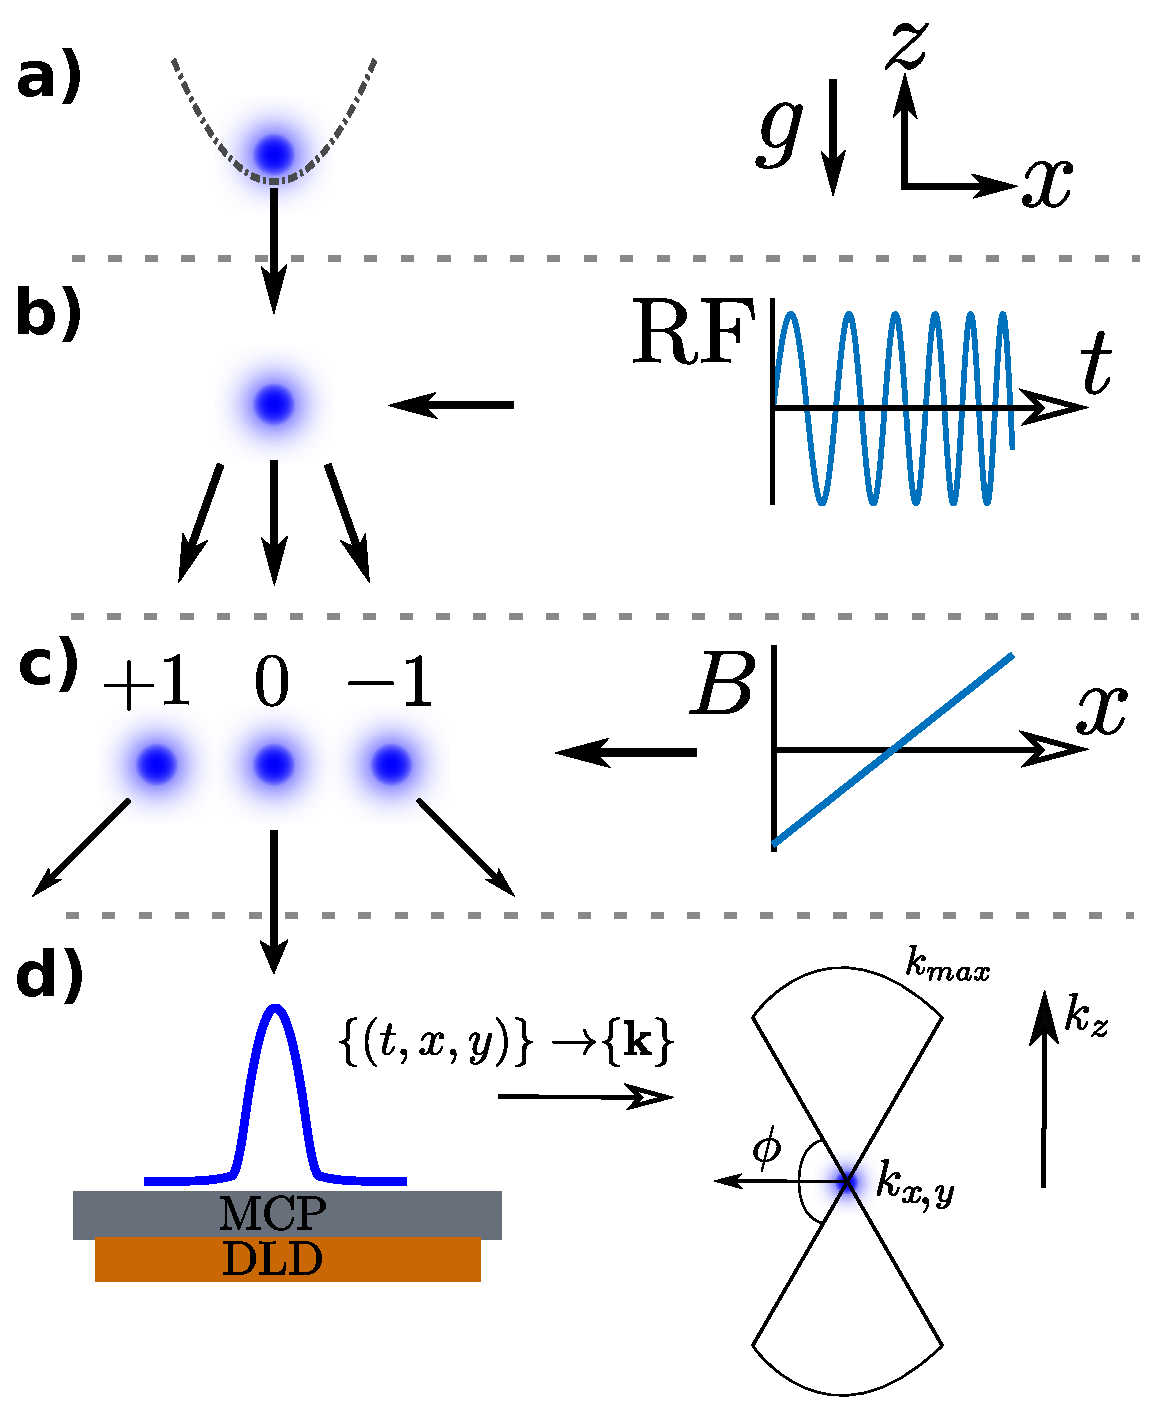
\includegraphics[width=0.4\textwidth]{fig/QD/exp_cartoon}
% %     \caption{Sketch of experimental sequence.
% 	A BEC is released from a harmonic trap (a) and expands during freefall before being split into a superposition of the $m_J\in\{-1,0,1\}$ states (b) by an RF chirp.
% 	A magnetic field gradient separates the clouds (c) ensuring that only the magnetically insentitive $m_J=0$ cloud lands on the detector (d), from which the momentum information is reconstructed.
% 	The quantum depletion lies in the dilute tails at large momentum (inset).}
% %     \label{fig:sequence}
% % \end{figure}


% % \begin{figure}[b]
% %         \includegraphics[width=0.5\textwidth]{fig/QD/contact_determination}
% %         \caption{The empirical density of particle momenta (a) for different peak densities, showing the transition between the condensed, thermal, and depletion regions (indicated for $n_0=20~\mu\textrm{m}^{3}$ with dotted lines).
% 	The number of atoms with wavevector $k\in\{k_1,k_2\}$ within the depletion region yields an estimate of the contact via Eqn.
% 	(\ref{eqn:c_est}).
% 	Fixing $k_2=10\mu\textrm{m}^{-1}$, we show $C_\textrm{est}$ as a function of the cutoff $k_1$ (b), which behaves consistently with a $k^{-4}$-like scaling of the momentum distribution.
% 	For each run we choose the $k_1$ at which $C_\textrm{est}$ is the most stable.}
% %         \label{fig:cdfplot}
% % \end{figure}

% % \section{Results} 
% % The single-particle detections can be used to construct an estimate of the far-field momentum density.
% 	However, estimating parameters of power-law distributions by fitting histograms is prone to bias and underestimation of uncertainties, especially when data is available over less than a decade of dynamic range \cite{clauset09,virkar14}.
% 	The preferred statistical tool for analysing power law distributions are maximum likelihood estimators \cite{goldstein04,clauset09,virkar14,hanel17}, but these are unavailable here because there are multiple sources of detection events, as detailed in \cite{SOM}.
% 	We present an approach that overcomes these issues, yielding the dependence of the tail amplitude on the condensate density in a straightforward way, along with a rigorous uncertainty estimate.
	

% % The Tan relations yield an expression for the asymptotic momentum density in terms of the \emph{contact} $\mathcal{C}$
% % \begin{equation}
% % \lim_{k\rightarrow\infty}\rho(k) = \frac{\mathcal{C}}{k^4}=\frac{64\pi^2a^2}{7} \frac{n_0 N_0}{k^4},
% % \label{eqn:mom_dist}
% % \end{equation}
% % where $n_0$ is the peak density of a condensate of $N_0$ atoms with s-wave scattering length $a$ \cite{tan08_energetics,tan08_momentum} (a detailed derivation is given in \cite{SOM}).
% 	Under the hypothesis that the \emph{in situ} depletion survives the expansion, one can integrate Eqn.
% 	(\ref{eqn:mom_dist}) to predict the expected number of atoms whose wavevector has a modulus in the interval $k\in (k_1, k_2)$, 

% % \begin{align}
% % \mathcal{N}_{k_1,k_2} &=\int_{k_1}^{k_2} \frac{\rho(k)}{(2\pi)^3}k^2~dk~d\theta~d\phi\\
% % 		&=\frac{\mathcal{C}}{2\pi^2}\left(\frac{1}{k_1}-\frac{1}{k_2}\right)
% % \label{eqn:pred_num}
% % \end{align}
% % where the $(2\pi)^3$ Jacobian ensures normalization in $k$-space.
% 	The inverse of Eqn.
% 	(\ref{eqn:pred_num}) thus yields an estimation of the tail amplitude (the contact)
% % \begin{equation}
% % C_\textrm{est} = \frac{2\pi^2N_{k_1,k_2}}{\eta}\cdot \frac{k_1 k_2 }{k_2-k_1},
% % \label{eqn:c_est}
% % \end{equation}
% % in terms the number of detected atoms $N_{k1,k2}$ and the total collection efficiency $\eta\approx0.3\%$, which accounts for the detector efficiency and geometric factors, as detailed in \cite{SOM}.
	

% % Fig.
% 	\ref{fig:cdfplot} (a) we show the empirical density $n(k)$ for three representative data collection runs.
% 	The three regimes of the condensate, thermal part, and depleted particles are visible, spanning over five orders of magnitude in density.
	

% % In Fig.
% 	\ref{fig:cdfplot} (b) we show the estimated contact $C_\textrm{est}$ as obtained from Eqn.
% 	(\ref{eqn:c_est}), as a function of the lower bound $k_1$ with $k_2=10~\micron^{-1}$.
% 	Indeed, Fig.
% 	\ref{fig:cdfplot} (b) and Eqn.
% 	(\ref{eqn:c_est}) provide a test for the presence of $k^{-4}$ scaling in the momentum density: Because Eqn.
% 	\ref{eqn:c_est} is derived assuming a $k^{-4}$ power law, any other behaviour would manifest as a clear dependence of $C_\textrm{est}$ on $k_1$.
% 	The invariance of $C_\textrm{est}$ in Fig.
% 	\ref{fig:cdfplot} therefore confirms the $k^{-4}$ power-law decay in the region of interest.
	

% % The value of $k_1$ must be determined for each run, as the crosssover over from thermal to quantum-depleted varies with the condensate density and temperature.
% 	We fix $k_1$ as the point where $dC_\textrm{est}/dk_1$ is minimized, ranging from $4.5-6.5\mu\textrm{m}^{-1}$ between runs.
% 	The uncertainty in the $C_\textrm{est}$ for each run is the standard error in the mean of $C_\textrm{est}$ over all the shots in that run.
% 	Across all runs, the average value of $C_\textrm{est}$ is 8(1) times \textit{in situ} predictions using Eqn.
% 	(\ref{eqn:pred_num}) and calibration parameters.
% 	The final uncertainty in this sensitivity is obtained by simple propagation of errors, avoiding the problem of total least-squares regression as encountered in the prior work \cite{chang16}.
% 	The empirical dependence of $C_\textrm{est}$ on the atom number and trapping frequencies is shown as a solid line in Fig.
% 	\ref{fig:results_comp}, with the uncertainty shown as a shaded area.
% 	Thus, while the observed momentum distribution is consistent with a $k^{-4}$ asymptotic decay, the amplitude of these tails contradicts the hypothesis of Eqn.
% 	(\ref{eqn:pred_num}) by 7$\sigma$.

    
% % 	\begin{figure}[t]
% % 	        \includegraphics[width=0.5\textwidth]{fig/QD/results_comp}
% % 	        \caption{Comparison of simulations and experiments.
% 	The inset is a zoomed view.
% 	 From our empirical data (ED) we determine the empirical contact $C_\textrm{est}$ which is linear in the product $N_0n_0$ (Eqn.
% 	(\ref{eqn:mom_dist})), but 8(1) times more sensitive (Av) than the prediction by the Tan theory (TT).
% 	The simulated contact of BECs in a cigar-shaped trap (CT) are consistent with (TT) before release and increases after expansion (CE), but by less than the experiment.
% 	A slow relaxation of the tight axes of the cigar trap (CS) leads to a reduction in the simulated contact.
% 	Simulations of a spherical trap (ST) show a negligible increase after expansion (SE).
% 	The prior \mhe result \cite{chang16} (IO) is shown for comparison (dashed line)}
% % 	        \label{fig:results_comp}
% % 	\end{figure}


% % 	\begin{figure}[b]
% % 	        \includegraphics[width=0.5\textwidth]{fig/QD/time_dep_theory}
% % 	        \caption{Simulations of condensates released from a cigar-shaped trap show an increase in contact after the trap release, stabilizing after a time on the order of $1/\omega_x$, several hundred $\mu$s.
% 	The relative difference between in-trap and expanded contact increases with the density of the condensate.
% 	For comparison, the experimental control pulses are implemented after 2ms of expansion.
% 	In contrast, when the transverse trapping frequencies are reduced by half (dotted line), the in-situ contact relaxes.}
% % 	        \label{fig:theory_time_dep}
% % 	\end{figure}
% % 	% \

% % 	\section{Simulations} To understand the excess contact here and in earlier experiments \cite{chang16}  
% % 	we performed simulations of the BEC expansion from harmonic traps using the first principles STAB method \cite{Deuar11,Kheruntsyan12}.
% 	The simulations included a cigar-shaped trap (marked CT in Fig.
% 	\ref{fig:results_comp}) with parameters matched to the experimental conditions (see \cite{SOM} for details).
% 	The in-trap state was consistent with the adiabatic sweep theorem before release from the trap.
% 	Following expansion from the cigar trap (CE), the simulated tail amplitude increased and stabilized at a factor of 1.64(9) above the predictions of Eqn.
% 	(\ref{eqn:mom_dist}).
% 	The steady-state occurs within a few hundred microseconds, much sooner than the 2ms delay between the trap release and application of the rf and Stern-Gerlach pulses.
% 	To understand the disagreement with earlier theory \cite{qu16}, which predicted no depletion survival, we also investigated the effect of adiabatic expansion on the in-trap depletion by simulating a slow decrease of the transverse trapping frequencies by a factor of two (CS), and found that the in-trap contact decreased roughly as predicted by Eqn.
% 	(\ref{eqn:mom_dist}) in these instances --- see the dashed line in Fig.~\ref{fig:theory_time_dep}.
% 	Details of the method and calculations are in supplementary material \cite{SOM}.
	

% % 	We interpret our results as an indication that the depleted atoms are accelerated by the non-uniform mean-field energy of the condensate during the expansion, and that this contributes to the disagreement between \emph{in situ} and measured contact.
% 	In detail, after a quench into the free particle regime, the condensate expands hydrodynamically on timescales of $1/\omega$.
% 	This is an adiabatic process for the low momentum depletion, whereby some depleted atoms are absorbed back into the condensate in agreement with \cite{qu16}.
% 	However, the characteristic time for reabsorption is $\hbar/gn_0$, slow enough that quasiparticles in the particle branch of the Bogoliubov dispersion have sufficient velocity to escape the expanding cloud without being reabsorbed and thus transition to free atoms.
	
	
% % 	Moreover, an atom inside the BEC experiences an effective force from the gradient of the mean-field potential $\textbf{F} = -4\pi\hbar^2a \nabla  n(x)/m$.
% 	This endows escaping depleted particles with a greater momentum, increasing the weight of the tails in the far-field.
% 	This effect is exacerbate in light atoms like $^{4}$He: because the acceleration scales with $1/m^2$, it would be suppressed by a $\sim500$-fold in $^{87}$Rb experiments \cite{makotyn14}.
% 	This picture is supported by our simulations, in which we observe a decrease in the total number of depleted particles (reabsorption) and a simultaneous increase of the large-k population (forcing).
% 	Further, it is much easier for depletion atoms to escape and be accelerated in the transverse x-y directions from an elongated cloud because the distances $R_{TF}=\frac{1}{\omega}\sqrt{2gn_0/m}$ are reduced by $\bar{\omega}/\omega_{x,y}$, whereas the initial mean depletion velocities \textit{in situ} $v\sim \sqrt{2gn_0/m}$ are isotropic: Indeed, spherical clouds (SE) exhibit a much weaker effect than the elongated clouds (CE) owing to the longer escape time.
	 

% % 	\section{Discussion} 
% % 	Our work expands the growing suite of far-field investigations of quantum depletion \cite{cayla20,chang16} and confirms that quantum depletion can, remarkably, survive past the lifetime of its original condensate.
% 	Our findings clarify that how the depletion can be visible in the far-field momentum distribution here and in earlier experiments, and that the hydrodynamic approximation does not capture sufficient short-wavelength information to make detailed predictions about the high-momentum behaviour.
% 	We thus find a partial explanation for the deviation of the far-field distribution from both the predicted in-situ depletion and the hydrodynamic reabsorption: The interplay between coherent absorption of Bogoliubov excitations and the dispersal of the chemical potential into kinetic energy, to which helium is particularly sensitive, result in a growth of the $k^{-4}$ tails of the momentum distribution during freefall.
% 	However, a mystery remains: Why is the excess depletion some four times greater than accounted for by this picture? This issue should be resolved in order to interpret far-field observations in terms of the in-trap physics of interest.
% 	This question invites complementary studies of the \emph{in situ} depletion in \mhe BECs.
% 	The important question of whether the far-field anomaly originates in the trapped state or during expansion would be best pursued with Bragg spectroscopy, given the complications of radio spectroscopy of Helium as discussed in \cite{SOM}.


% % \section{Detection}

% % 	We use a Roentdek DLD80 multichannel plate and delay-line detector stack \cite{Manning10} with a quantum efficiency of $\approx8\%$, and space and time resolutions of 100 $\mu$m and 3 $\mu$s, respectively \cite{Henson18}.
% 	After the atoms are released from the trap, they fall 859mm to the detector stack, which registers the arrival times and positions $(t_i,x_i,y_i)$ of each atom, indexed by $i$.
% 	The centre of mass of the cloud arrives after a $\tau = 417$ms time of flight following the trap switch-off.
% 	The velocity of each atom relative to the centre of mass of the cloud is given by $(v_x,v_y,v_z) = t_{i}^{-1}(x_i-\bar{x},y_i-\bar{y},g_0(\tau^2-t_{i}^{2}))$, where $g_0$ is the local gravitational acceleration and the overbar denotes the within-shot average.
% 	The velocity conversion assumes a point source but carries a negligible error of a few ppm as the in-trap BEC size is smaller than the detector resolution.
% 	We centre the counts from each realization and detection sequence (termed a \emph{shot}) and transform the counts from cartesian velocity space to spherical polar coordinates with radius $k$ (in $m^{-1}$), polar angle $\theta$ and elevation angle $\phi$, relative to the centre of the cloud, where the velocity-to-wavevector transformation follows from  $\textbf{p}=m\textbf{v}=\hbar\textbf{k}$.
	



% % 	The detector efficiency was $\chi=0.08(2)$, as we determined from the collection efficiency of correlated atoms on the opposite sides of scattering halos \cite{shin19,shin20,Jaskula10}.
% 	The solid angle in k-space available to detect the depleted tails is limited by the 40mm radius of the circular detection surface.
% 	The field of view of our detector in the $(x,y)$ plane is $\lesssim5\times 10^6$ m$^{-1}$, which is only just sufficient to reach past the edge of the thermal region.
% 	Therefore, we sample data from the segments of the sphere with elevation angle $|\phi|>\pi/3$ rad and $|k|<10^7$ m$^{-1}$, centred on the BEC, which encompasses a total solid angle of $0.13\times 4\pi$ steradians.
% 	The noise floor is set by the detector's dark count rate of $0.56(1)$ Hz cm$^{-2}$, which contributes an average of 0.4(2) counts to the region of interest (ROI) per shot.
% 	 A summary of the results for each data run are shown in Tab.
% 	\ref{tab:results}.






% % % \todo{Density plots out to larger $|k|$ to show descent into noise floor? How far could we push it until we hit dark counts?}

% % % \section{Spin mixing}
% % % Also lets us determine thermal fraction - note it isn't determinable from the PAL because of the mean-field broadening (but one could just make fits and subtract the thermal part, yes?).
% 	I think the mean-field expansion is particularly bad for Helium, and wasn't reported much before, because we are 5% the mass of popular species like Rb so much more subject to mean-field acceleration!

% % \section{Trap configuration and calibration}

% % 	We prepared our BECs with via forced evaporative cooling in a harmonic magnetic trap with trap frequencies $(425,425,45)$ Hz and a DC bias stabilized by our auxiliary field compensation coils \cite{Dall07,Dedman07}.
% 	For the tight trap we increased the coil current after the cooling sequence to obtain trapping frequencies $(902,895,71)$ Hz, ramping the field as a sigmoid step function to minimize in-trap oscillations.
% 	The trap remained on for 150ms before switching the trap off with a $1/e$ time of $\approx38\mu$s.
% 	The condensates were allowed to expand for 2ms before we transferred some of the condensate into the magnetically insensitive $m_J=0$ state via Landau-Zener sweep to prevent distortion by stray magnetic fields.
% 	The RF pulse was created by a  function generator, amplified, and applied to the experiment chamber by a coiled antenna inserted into the BiQUIC coil housing.
% 	The pulse swept from 1.6-2.6MHz over 1ms and was centred on the fine structure resonance between the $m_J$ states.
% 	The transfer efficiencies $\eta_j$ for each of the $m_J = j$ states is discussed in the next section.
% 	The sweep was $10^6$-fold wider than the Doppler broadening of the BEC which ensured uniform transfer at all momenta.
% 	Immediately after the RF sweep, the bias coils are switched off and auxiliary push coils in the vertical (Z) and weak horizontal (X) axes are activated using a fast MOSFET switch to implement a Stern-Gerlach separation of the $m_J = -1,~0,$ and $+1$ pulses.

% % \subsection{Determining transfer efficiency}

% % 	To calibrate the transfer efficiencies, we applied a weaker Stern-Gerlach than for the depletion measurement, resolving each $m_J$ cloud on the detector, as illustrated in Fig.
% 	\ref{fig:frac_cal}.
	

% % \begin{figure*}[!t]
% % 	\begin{center}
% % 		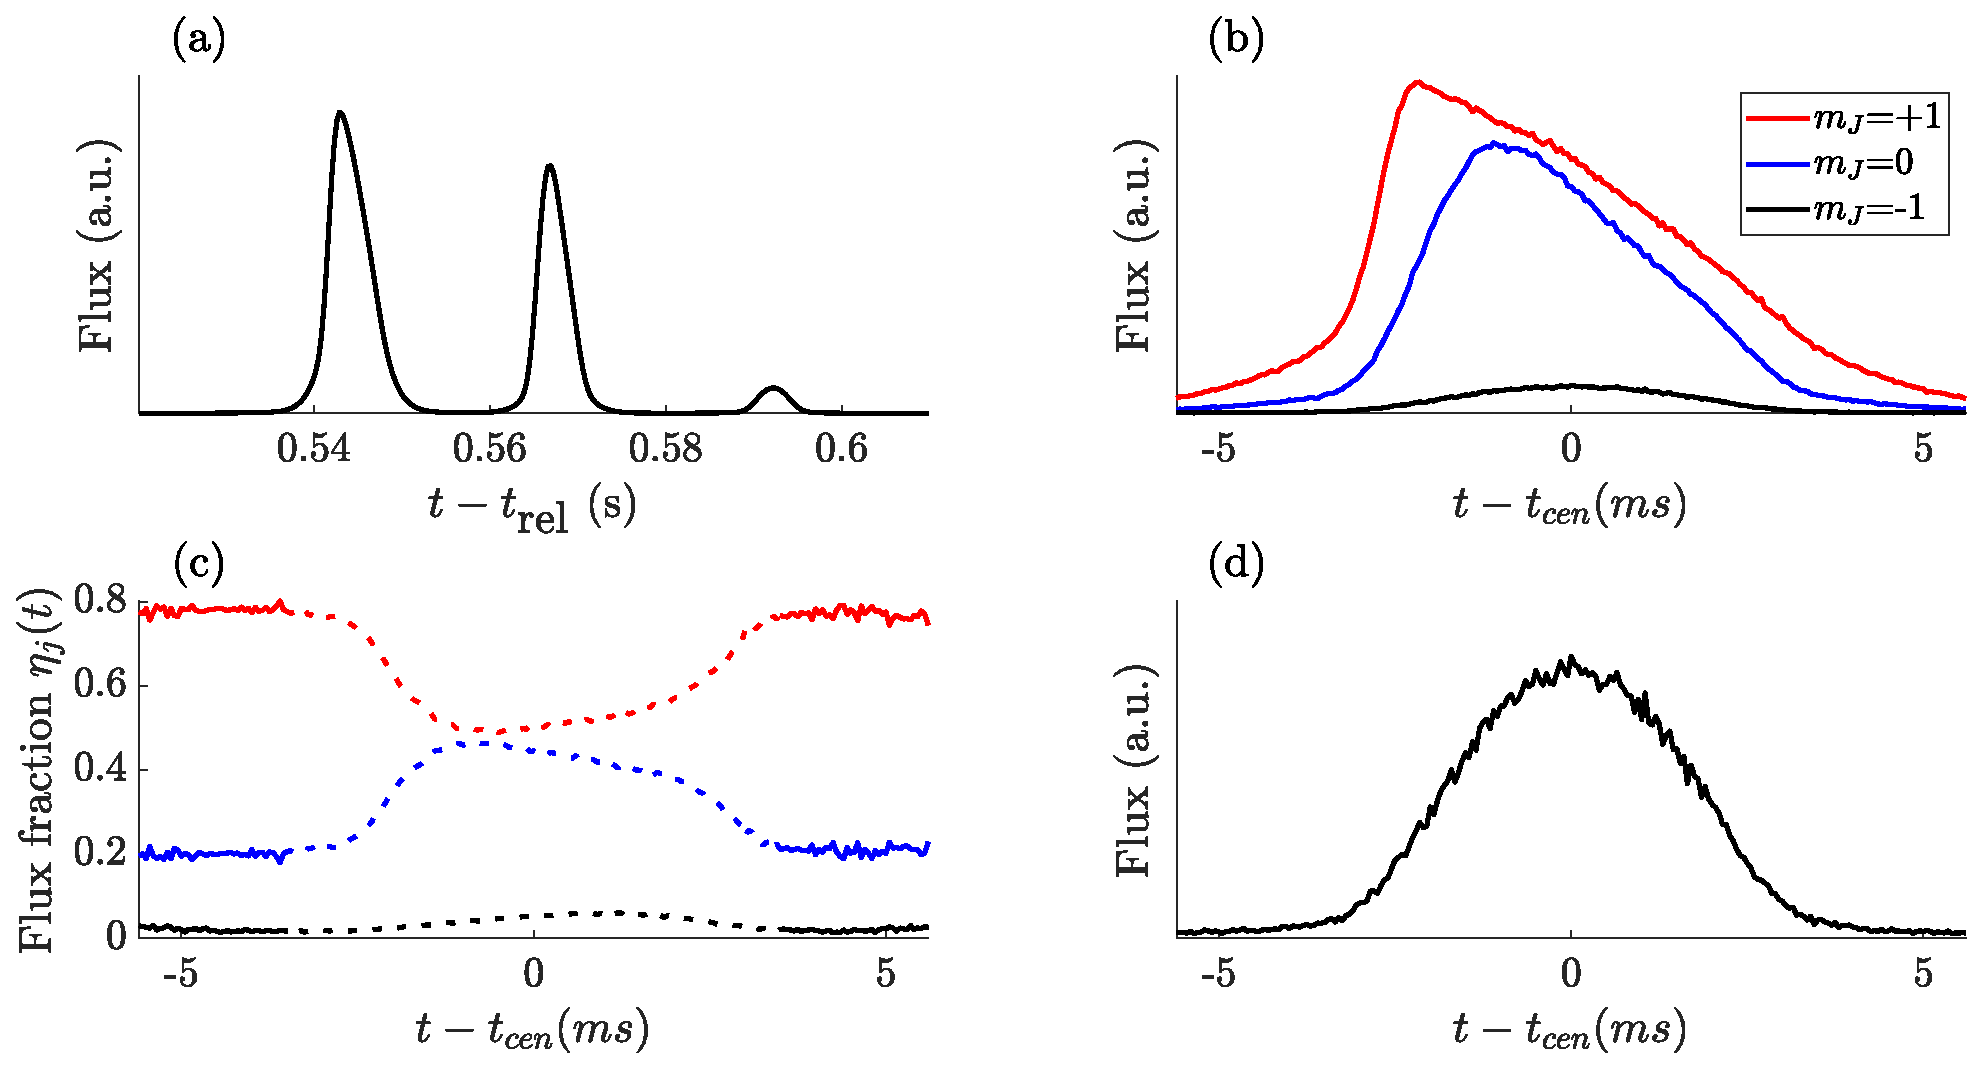
\includegraphics[width=\textwidth]{fig/QD/frac_cal_profile}
% % 		\caption{Determining the RF transfer efficiency.
% 	The time-of-flight profiles of each pulse are resolved (a) by applying a weak Stern-Gerlach pulse during the time of flight.
% 	The pulses are aligned with respect their centre-of-mass (b) and used to determine the pointwise fraction ((c), dotted line).
% 	Detector saturation is evident in the peaks (dashed lines), but not in the thermal tails (solid lines), which are used to compute the transfer efficiency.
% 	Because of its lower flux, the $m_J=-1$ pulse does not show evidence of saturation (d) and is used to determine the thermal fraction.}
% % 		\label{fig:frac_cal}
% % 	\end{center}
% % 	\end{figure*}

% % 	The efficiencies $\eta_J$ cannot be calculated by counting the atoms in each cloud because the detector saturates during the peak condensate flux, but we can compare the thermal parts.
% 	We align each cloud along the time (Z) axis and compute the pointwise fraction of the atomic flux $\phi(t)$ accounted for by each cloud, $\eta_j(t) = \phi_j(t)/\sum_j\phi_j(t)$, as depicted in Fig.
% 	\ref{fig:frac_cal}.
% 	The ratio of densities between the clouds is roughly constant in the thermal part, indicating the absence of important saturation effects and a spin transfer that is independent of $k$.
% 	The fraction of the original cloud transferred into each $m_J$ state is determined by taking the average $\langle\eta_j(t)\rangle$ over the thermal tails.
% 	We find these efficiencies are approximately 74\%, 24\%, and 2\% in all runs for the $m_J=+1$, 0, and -1 states, respectively.
	
% % 	While the $m_J=0$ and $m_J=1$ clouds clearly saturate the detector, the small fraction ($\approx2\%$) of the atoms transferred to the $m_J=-1$ state does not (Fig.
% 	\ref{fig:frac_cal} (d)).
% 	A bimodal fit to the condensed and thermal parts, plus constant background, yields an estimate of the thermal and condensed fractions.
	


% % % \subsection{Determination of thermal fraction}
	

% % % 	\begin{figure}[!h]
% % % 	\begin{center}
% % % 		\includegraphics[width=0.8\textwidth]{fig/QD/m1_frac_anal}
% % % 		\caption{Comparison of thermal fits in the unsaturated $m_J=-1$ pulse including 138 shots.
% 	The weak (X) and strong horizontal (Y) trapping axes are shown in (a) and (b), respectively.
% 	\org{would be helpful to label $v_x$ and $v_y$ to make it self-evident at 1st glance.} Both projections display a bimodal peak, with the condensate (dotted lines) and thermal parts (thick solid lines) easily distinguished.
% 	Fitting a Gaussian profile (thin solid line) to the velocity distribution of the thermal part yields the thermal number and temperature.
% 	Subtracting the fit leaves the condensate profile (c) which can be \blu{\dots something\dots} yields the condensed number.}
% % % 		\label{fig:thermal_frac}
% % % 	\end{center}
% % % 	\end{figure}



% % \subsection{Analysis of spin transfer measurements}

% % 	In early tests of our measurement sequence we noticed a contamination of the signal by spurious counts.
% 	We inferred these were remnant counts from the $m_J=+1$ cloud as they were still visible when we ran an experimental sequence without the Landau-Zener transfer.
% 	This contamination appeared in a particular region of our detection image, illustrated in Fig.
% 	\ref{fig:spinpop}.
% 	As such we were able to correct for it by subtracting their contribution from the counts collected during measurement shots.
% 	Generally, fewer atoms can be attributed to this noise than would be required to explain the discrepancy described in the main text, as illustrated in Fig.
% 	\ref{fig:num_counts}.
% 	While the cause of the cross-contamination is unclear, we observe that the count density outside the region of interest is similar in both the shots with the RF pulse and those without.
% 	We hypothesize that the remnant counts are atoms transferred into the $m_J=0$ state by non-ideal behaviour of the Stern-Gerlach pulses.
	

% % 	As mentioned in the main text, the presence of these counts also prevents a straightforward application of a maximum-likelihood estimator (MLE) to determine parameters of the power-law region.
% 	The basic principle of the MLE is to assume a functional form for the probability distribution $p(x|\theta)$ underlying the observed data $x$, and dependent on some parameters $\theta$; the zero of the derivative of the \emph{likelihood} function $L(\theta|x)$ with respect to the parameters $\theta$ then yields the most-probable parameter values given a set of observations $x$.
% 	In our context, one can assume a functional form for the probability distribution underlying atomic detection events (via a wavefunction ansatz).
% 	The detector dark count rates can also be incorporated by assuming a uniform distribution.
% 	Such an analytical treatment does not readily permit the inclusion of an empirical density estimate which itself includes the aforementioned dark count rate.
% 	Instead, we opt for the simpler approach described in the main text.

% %     \begin{figure}[!b]
% % 	\begin{center}
% % 		\includegraphics[width=\columnwidth]{fig/QD/spinpop}
% % 		\caption{Measured contribution of the detector dark counts and spurious spin counts to the time-of-flight profile.
% 	We accounted for the pulse at around 550ms and subtracted it from the measured profiles when computing the contact.
% 	After removing this background term, the density profiles above and below the condensate agree, indicating convergence on the true signal.
% 	For reference, the peak flux of the $m_J=0$ condensate is about a thousandfold greater than the peak shown here.}
% % 		\label{fig:spinpop}
% % 	\end{center}
% % 	\end{figure}

% % 	% \begin{figure}[!h]
% % 	% \begin{center}
% % 	% 	\includegraphics[width=\textwidth]{fig/QD/profile_overlay}
% % 	% 	\caption{Comparison of average time-of-flight profiles over a single data run for the quantum depletion measurement shots (blue, 871 shots), transfer efficiency calibration (black, 112 shots), detector dark counts (red, 871 shots), and spurious counts (dot-dash, 895 shots).
% 	The time window bounded by $|k|\leq 10\mu$m is indicated with dotted lines.
% 	Shaded area is the standard error over the entire run.}
% % 	% 	\label{fig:tof_profile}
% % 	% \end{center}
% % 	% \end{figure}




% % % Note that the temps disagree between axes, but within axes between clouds they are consistent(....ish).
% 	This means we can use the profile ratio method, which is also consistent with comparing the thermal number from the fits.
% % % Perhaps comment on the thermal-subtracted part; the TF profile should have a sharp cutoff, but the smooth edges are suggestive evidence of this roll-off

% % \begin{figure}
% % 	\centering
% % 	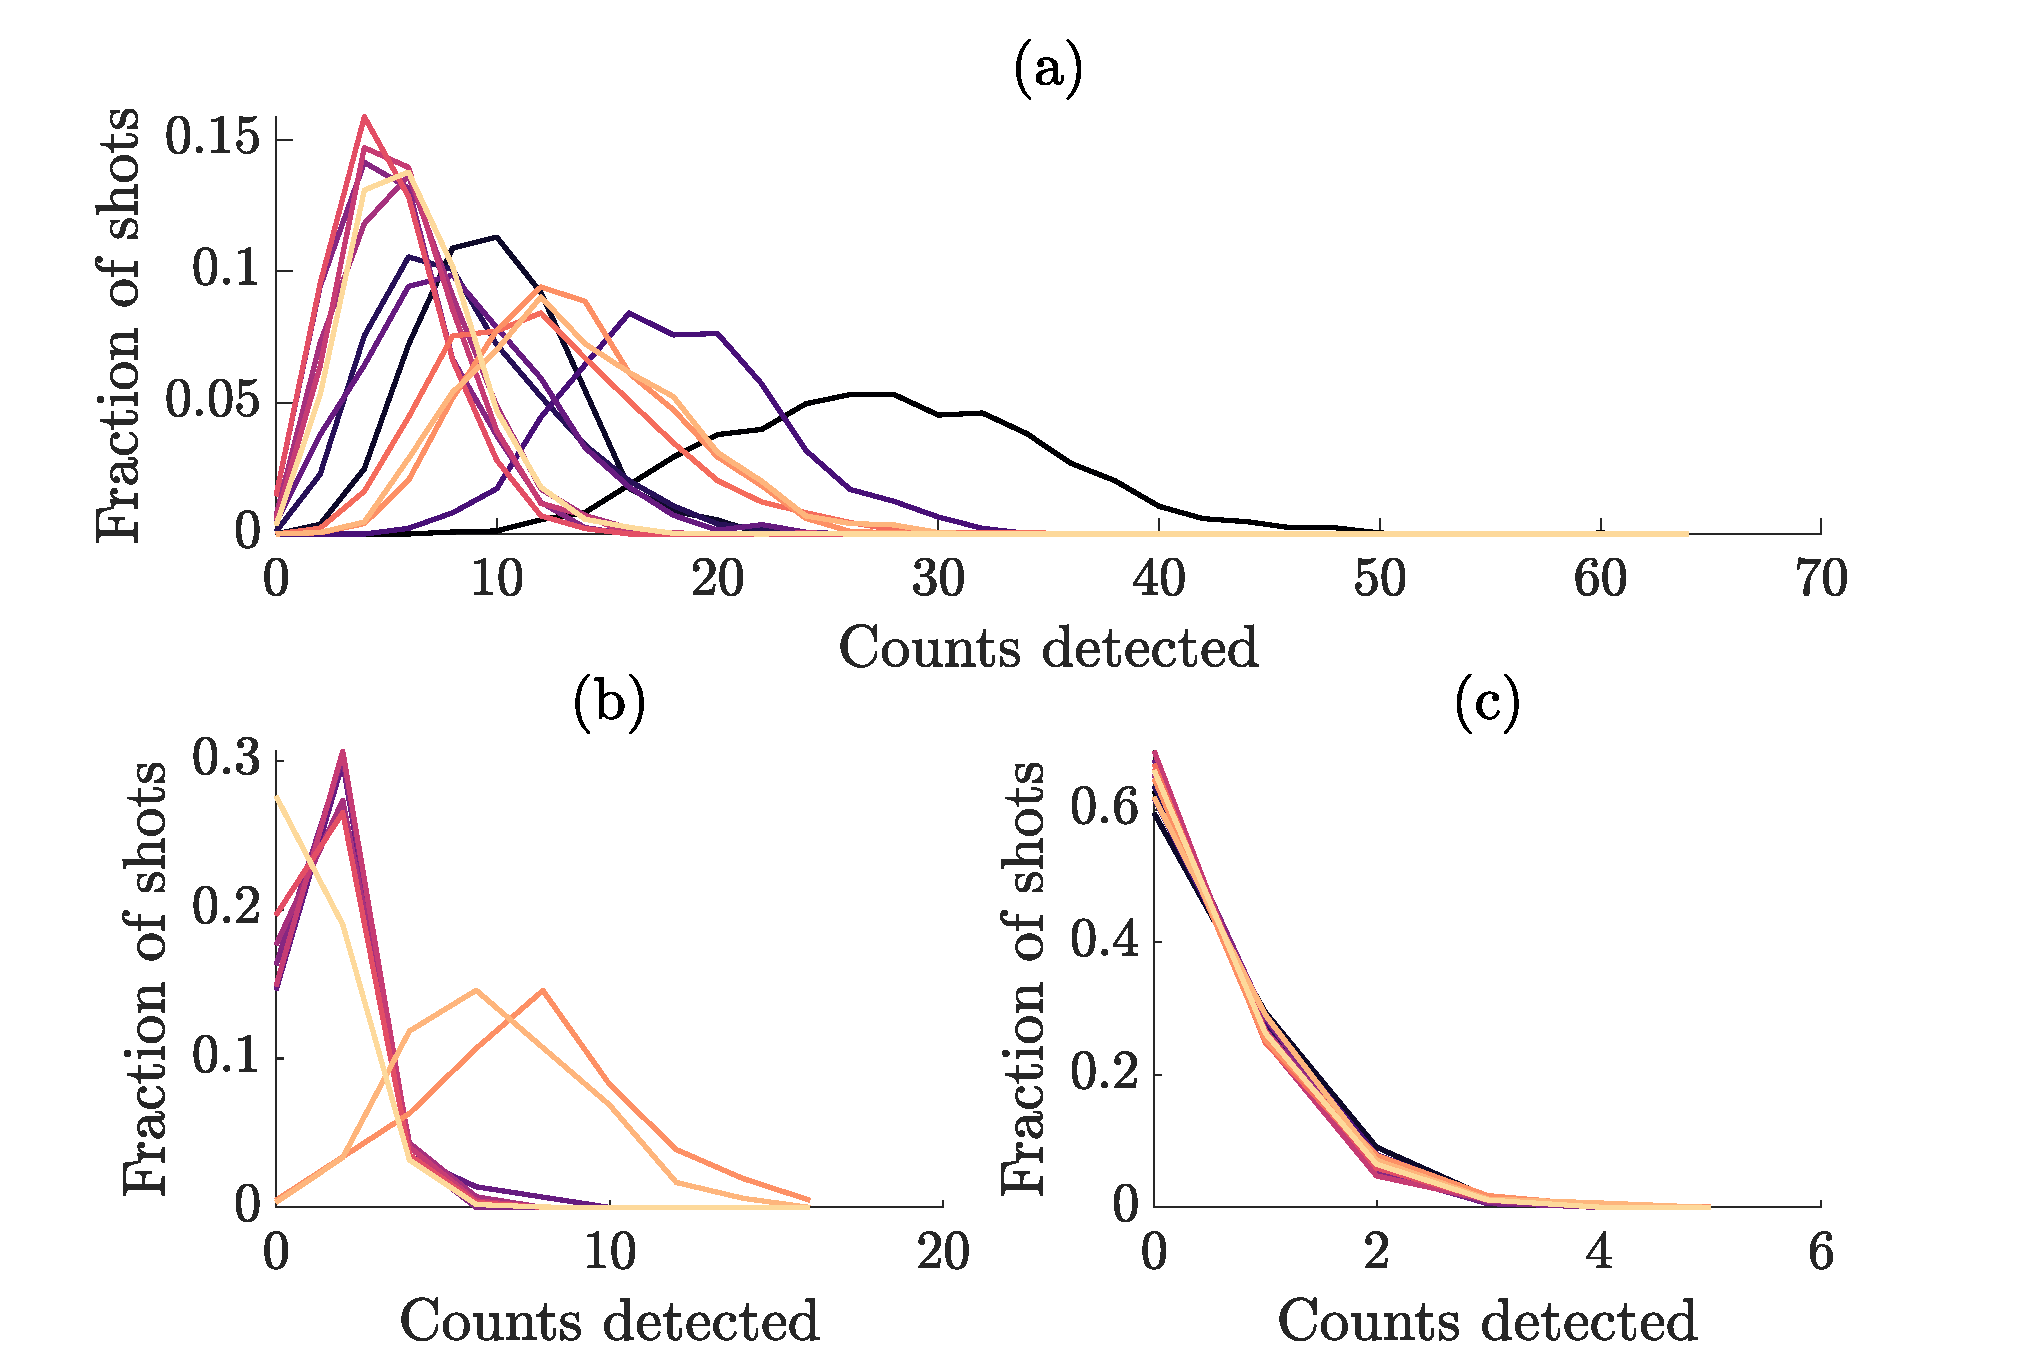
\includegraphics[width=0.5\textwidth]{fig/QD/counts_per_run}
% % 	\caption{Number of counts detected in the region of interest in the depletion measurement (a), the spin mixing calibration (b), and the dark count calibration (c).
% 	An average of 3.0(5) counts were detected in the ROI in the spin-mixing calibration shot, and the background count rate was 0.4(2) counts per shot.
% 	Separate lines indicate separate \emph{runs}, i.e.
% 	sequences of shots with fixed parameters.}
% % 	\label{fig:num_counts}
% % \end{figure}


% % \subsection{Peak density calibration}

% %     The quantum depletion and contact are both predicted to depend solely on the condensed number and trapping frequencies via the condensate density, hence it is important to determine both quantities accurately.
% 	In the Thomas-Fermi approximation, the peak density of the condensate can be written as $n_0 = \mu/g$, where $\mu$ is the chemical potential, $g=4\pi\hbar^2a_{1,1}/m$ is the effective interaction strength, $m\approx6.6\times10^{-27}$ kg is the atomic mass, and $a=7.512$ nm is the s-wave scattering length between pairs of atoms in the $m_J=1$ state \cite{Moal06}.
% 	The expression for the peak density can be expanded as
% % 	\begin{equation}
% % 		n_0 = \frac{1}{8 \pi}\left( (15N_0)^2 \left(\frac{m \bar{\omega}}{\sqrt{a_{1,1}} \hbar}\right)	 ^{6}\right)^{1/5}
% % 		\label{eqn:n0}
% % 	\end{equation}
% % 	where $\bar{\omega} = \left(\omega_x\cdot\omega_y\cdot\omega_z\right)^{1/3}$ is the geometric trap frequency and $N_0$ is the number of atoms in the condensate.
% 	During these calibration runs we simultaneously determine the total atom number $N$ and trap frequency $\bar{\omega}$ in a single shot using a pulsed atom laser and use the thermal fraction to determine the condensed number $N_0$.
	

% % 	The pulsed atom laser consists of a series of Fourier-broadened RF pulses centred on the minimum Zeeman splitting in the trap.
% 	The pulse transfers atoms in the trap to the untrapped $m_J=0$ state with an approximately constant transfer rate across the cloud.
% 	We outcouple approximately 2\% of the atoms per 100$\mu$s pulse for $\approx$200 pulses, which eventually depletes the entire trap.
% 	The atom laser thus prevents the detector from saturating and allows an accurate determination of the atom number, up to a factor of the quantum efficiency.
% 	We determine the trapping frequencies by inducing centre-of-mass oscillations with a magnetic impulse, and finding the oscillation period from the atom laser pulses \cite{henson18ML}.

% % % 	\begin{figure}[!h]
% % % 	\centering
% % % 		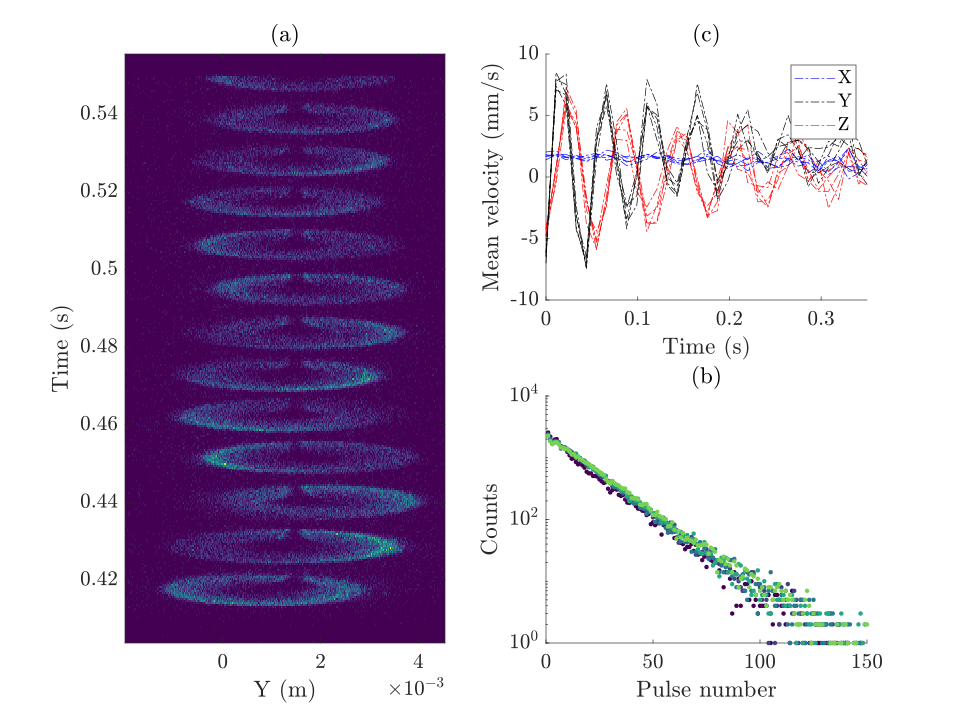
\includegraphics[width=0.8\textwidth]{fig/QD/pal_shot}
% % % 		\caption{A kicked pulsed atom laser with motion sampled at 11ms intervals.
% 	The oscillations in the centre-of-mass position of each pulse are shown along the Y axis over time (a).
% 	The apparent frequency can be determined for each axis (b).
% 	The outcoupling efficiency is fixed throughout the sampling sequence (c), producing a geometric decay of the number of atoms in each pulse.
% 	The straight line on a logarithmic scale shows that detector saturation saturation is negligible and that the BEC population does not affect the transfer rate.}
% % % 		\label{fig:pal_shot}
% % % 	\end{figure}
	
% % % \subsection{Measuring the trapping frequencies}

% % % 	To illustrate how we obtain the trapping frequencies, consider an undamped harmonic oscillator in one dimension.
% 	The centre-of-mass momentum $p(t) = A \cos(2\pi f t))$ oscillates at a frequency $f$ Hz, and the centre of mass of a pulse outcoupled at time $t'$ lands on the detector at a position $x'(t+\tau) = p(t')\tau/m$, where $\tau$ is the time of flight of the centre of mass.
% 	Sampling the cloud motion with a sampling period T starting at initial time $t_0$ produces a series of pulses whose centres of mass land at $\{x_n = (A\tau/m) \cos(\omega(t_0+nT))\}$.
% 	The sampling frequency $f_s=1/T$ determines the \emph{Nyquist frequency} $f_N=f_s/2$, which is the maximum frequency that can be reconstructed unambiguously from such a sampling regime.
% 	When $f>f_N$ the signal manifests as a lower-frequency oscillation known as the \emph{alias} of the signal.
% 	The aliased frequency $f_a$ is

% % % 	\begin{equation}
% % % 	 f_a =
% % % 	  \begin{cases}
% % % 	   \frac{Z_n f_s}{2} - f & \text{if } Z_n \text{ even} \\
% % % 	   f - \frac{(Z_n-1)f_s}{2}       & \text{if } Z_n \text{ odd},
% % % 	  \end{cases}
% % % 	  \label{eqn:Z_N}
% % % 	\end{equation}
	
% % % 	where $Z_n = \lceil{f/f_N}\rceil$ is the Nyquist zone number, as described in numerous RF engineering references.\org{Indeed ;-) probably needs rephrasing though}.
% 	While it is not possible to determine $Z_N$ for a signal with an unknown (not necessarily stationary) $f$ from samples taken at a fixed $f_s$, one can vary $f_s$ and determine both $Z_N$ and $f$ from the gradient $d f_a / d f_s$.
	
% % % \begin{figure}[!h]
% % % 	\centering
% % % 		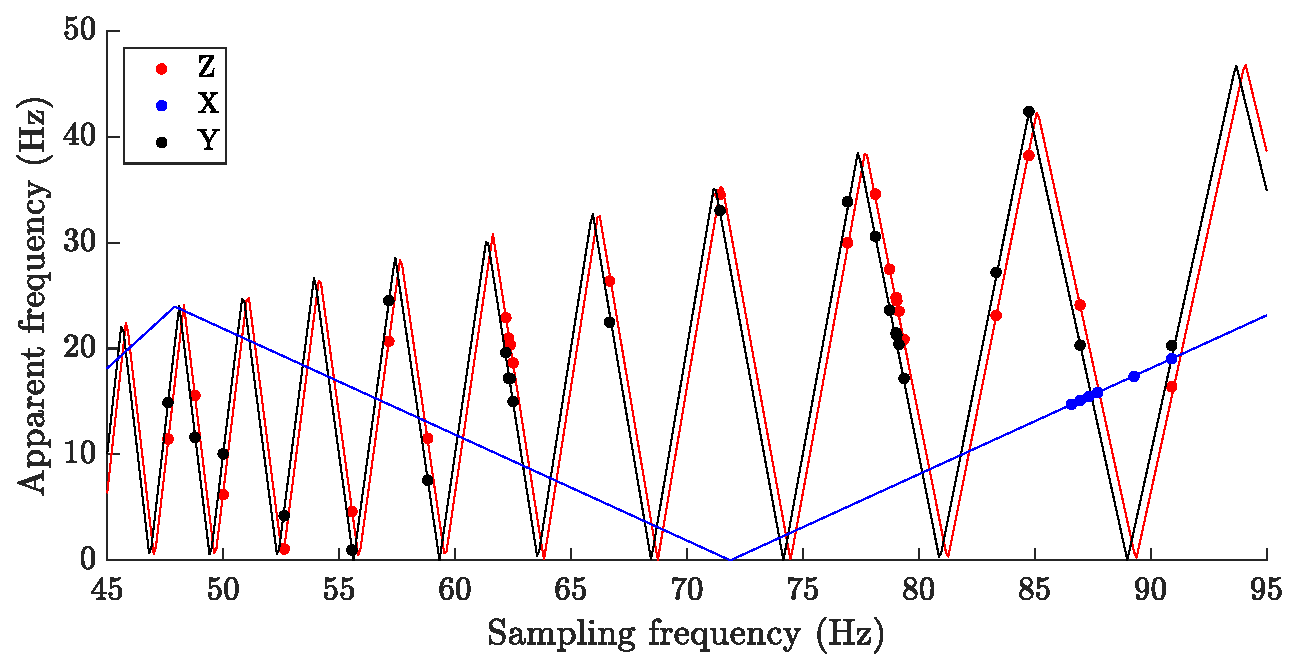
\includegraphics[width=0.8\textwidth]{fig/QD/sawtooth_plot}
% % % 		\caption{Aliasing of the trap frequency oscillations under different sampling regimes.
% 	The fitted oscillation frequency is shown in each axis for a range of sampling frequencies.
% 	The sawtooth function is a one-parameter fit which determines the underlying frequency of the centre-of-mass oscillations.}
% % % 		\label{fig:sawtooth_plot}
% % % 	\end{figure}	

% % % 	We induce oscillations of the BEC in all three axes by briefly displacing the trap centre with a perturbation to the trapping field.
% 	The maximum sampling frequency is limited by the temporal width of the BEC pulse landing on the detector to about 100Hz, yielding a Nyquist frequency too low to resolve the un-aliased oscillations.
% 	We fit the apparent oscillation frequency in each axis as a function of sampling frequency as shown in Fig.
% 	\ref{fig:sawtooth_plot}, along with a one-parameter fit of Eqn.
% 	\ref{eqn:Z_N}.
% 	\blu{We thus} determine that the frequencies $(\omega_x,\omega_y,\omega_z)$ of each of the traps used in the experiment are $2\pi\times(45,425,425)$ and $2\pi\times(72,889,893)$, respectively, which are stable to within 5\% throughout the duration of the data collection and to better than $1\%$ in a given run.


% % \begin{table*}
% % 	\begin{tabular}{c c c c c c c}
% % 	\hline\hline
% % 	Peak density ($\micron^{-3}$) & $N_\textrm{tot}$ ($\times10^5$) & Thermal fraction & $N_\textrm{Detect}$ & $N_\textrm{pred}$ & $C_\textrm{est}$ (pm$^{-1}$)  &$C_\textrm{est}/\mathcal{C}$  \\ 
% % 	\hline 
% % 	16(1) & 3.5(4) & 0.09 & 5.6(0) & 0.7(1) & .2(1)& 7(3) \\ 
% % 	18(1) & 5.0(4) & 0.17 & 6.8(1) & 0.9(2) & .2(1)& 7(2) \\ 
% % 	19(2) & 4.9(6) & 0.08 & 8.1(1) & 1.0(2) & .3(1)& 7(3) \\ 
% % 	20(1) & 5.7(3) & 0.09 & 14.(1) & 1.3(3) & .5(1)& 10(3) \\ 
% % 	38(2) & 3.9(3) & 0.14 & 4.9(0) & 0.4(1) & .6(3)& 10(5) \\ 
% % 	38(3) & 3.7(4) & 0.09 & 3.5(0) & 0.4(1) & .4(2)& 7(4) \\ 
% % 	38(3) & 3.8(4) & 0.11 & 3.7(1) & 0.6(1) & .4(2)& 6(3) \\ 
% % 	38(3) & 3.7(4) & 0.09 & 4.1(0) & 0.5(1) & .5(2)& 7(4) \\ 
% % 	39(4) & 3.8(5) & 0.10 & 4.3(0) & 0.5(1) & .5(3)& 7(4) \\ 
% % 	41(2) & 4.5(4) & 0.12 & 6.5(1) & 0.6(1) & .8(4)& 9(5) \\ 
% % 	\hline\hline
% % 	\end{tabular}
% % 	\caption{Summary of results for each data run.
% 	The peak density is determined from measurements of the condensed number (via the total number $N_\textrm{tot}$ and condensate fraction) and trapping frequencies, which in turn is used to predict the contact $\mathcal{C}$.
% 	The number $N_\textrm{Detect}$ of atoms detected in the region of interest can be used to determine the empricial contact $C_\textrm{est}$ from the $k^{-4}$-like tail, as in the main text, and can be compared to the predicted number of counts $N_\textrm{pred}$.
% 	The final column shows the ratio of the estimated to predicted contact, also equal to the ratio of the detected and predicted counts.}
% % 	\label{tab:results}
% % \end{table*}

% % \section{Theory}

% % The Hamiltonian of a homogeneous system of interacting bosons, with plane-wave field operators $\hat{a_\kvec}$ labeled by the wavevector $\kvec=\textbf{p}/\hbar$, can be diagonalized by the Bogoliubov transformation to a free Bose gas of collective excitations with operators $\hat{b}_\kvec$ \cite{Bogolubov47}.
% 	This permits the single-particle momentum density to be written as $\rho(k) = \langle\hat{a}_\kvec^\dagger\hat{a}_\kvec\rangle=\left(u_{\kvec}^{2}+v_{\kvec}^{2}\right)\langle b_{\kvec}^{\dagger}b_{\kvec}\rangle + v_{\kvec}^{2}$, where $\hat{a}_\kvec = u_\kvec \hat{b}_\kvec + v_{-\kvec}\hat{b}^\dagger_\kvec$, $\hat{a}^\dagger_\kvec = v_\kvec \hat{b}_\kvec + u_{-\kvec}\hat{b}^\dagger_\kvec$ and the $u_\kvec$ and $v_\kvec$ terms are fixed by the condensate density, atomic mass, and s-wave scattering length \cite{PitaevskiiStringari,PethickSmith}.
% 	In the ground state, devoid of thermal excitations, the quasiparticle modes are populated by the $v_{\kvec}^{2}$ term \cite{decamp18,chang16}.

% % While the local-density approximation (LDA) can be employed to compute the amplitude of the $k^{-4}$ tail using the Bogoliubov disperson \cite{chang16}, the approach opened by Tan's original theorems is simpler than integrating $v_\kvec^2$ across a Thomas-Fermi distribution.
% 	The two-body contact is defined by \cite{tan08_momentum}
% % \begin{equation}
% % \mathcal{C} = \lim_{k\rightarrow\infty}k^4\rho(k),
% % \label{eqn:MomentumDef}
% % \end{equation}
% % where the contact $\mathcal{C}$ is the volume average of the local \emph{contact intensity} $\hat{C} = 32 \pi^2 a^2 \hat{n}^2$ \cite{werner12_boson}.
% 	The contact is related to the total energy $E$ through the \emph{adiabatic sweep theorem} \cite{tan08_energetics},
% % \begin{equation}
% % \mathcal{C} = \frac{8\pi m a^2}{\hbar^2}\frac{\partial E}{\partial a},
% % \end{equation}
% % where $a$ is the s-wave scattering length.
% 	In the Thomas-Fermi approximation, the energy per particle of $N_0$ condensed bosonic atoms is 
% % \begin{equation}
% % \frac{E}{N_0} = \frac{5}{7}\mu = \frac{5}{7} \frac{\hbar \bar{\omega}}{2} \left(\frac{15 N_0 a}{a_\textrm{HO}}\right)^{2/5},
% % \label{mu}
% % \end{equation}
% % where $a_\textrm{HO} = \sqrt{\hbar/(m \bar{\omega})}$ is the harmonic oscillator length and $\bar{\omega}=\sqrt[\uproot{2}\scriptstyle 3]{\omega_x \omega_y \omega_z}$ is the geometric trapping frequency \cite{PitaevskiiStringari,PethickSmith}.
% 	The sweep theorem yields
% % \begin{equation}
% % \mathcal{C} = \frac{8\pi}{7} \left(15^{2}(a N_0)^{7} \left(\frac{m \bar{\omega}}{\hbar}\right)^{6}\right)^{1/5},
% % \label{eqn:TotalHarmonicContact}
% % \end{equation}
% % which shares many factors with the peak density of a harmonically trapped condensate (Eqn.
% 	\ref{eqn:n0}), whereby one has
% % \begin{equation}
% % 	\frac{\mathcal{C}}{n_0} = \frac{64\pi^2a^2}{7} N_0.
% % \end{equation}

% % By substitution into Eqn.
% 	(\ref{eqn:MomentumDef}) one arrives at the expression

% % \begin{equation}
% % \rho(k) = \frac{64\pi^2a^2}{7} \frac{N_0n_0}{k^4}
% % \end{equation}

% % Higher-order effects are negligible in our experiments.
% 	The Lee-Huang-Yang (LHY) corrected condensate energy $E'$ for a uniform condensate with density $n$ yields an estimate of the worst-case contribution
% % $$
% % \frac{\partial E'}{\partial a} = \mathcal{C}\left(1+\frac{64\sqrt{na^{3}}}{3\sqrt{\pi}}\right),
% % $$
% % Where $\mathcal{C}$ is the contact computed neglecting the LHY term, and the second term in brackets is the LHY correction which amounts to at most a correction of order 1\%, using the highest $n_0$ observed in our experiments.
% 	In reality the correction will be smaller as the density is not uniform and is bounded above by $n_0$.


% % \subsection{Radio spectroscopic prospects}
% % The cause of the contact anomaly could be elucidated by determining whether it originates in the trapped condensate, or is generated during the trap release and expansion.
% 	Such an investigation requires an \emph{in situ} probe of the contact, such as the radio and Bragg spectroscopic techniques.
% 	The latter may be the most fruitful of the two simply because of the difficulty of interpreting the results from the former, which we sketch below.
% 	The basic principle of RF contact spectroscopy is to apply a monochromatic RF probe which is detuned from the resonance between two spin states, coupling atoms in the initial spin state to an untrapped channel, and then perform a differential measurement of the atom number.
% 	The signal strength scales with the difference of reciprocal scattering lengths $\Gamma\propto(1/a_\textrm{i,i}-1/a_\textrm{i,f})$ between pairs of atoms in initial-initial ($a_{i,i}$) and initial-final ($a_{i,f}$) spin states \cite{braaten10,wild12}, which can be manipulated via Feshbach resonance to obtain a good signal.
% 	For He$^*$ (spin 1) however, the scattering lengths $a_{1,1}$ and $a_{1,0}$ are identical \cite{Leo01}, rendering the preferred $m_J=1-m_J=0$ transition unusable.
% 	On the other hand, $a_{1,-1} = 3/7 a_{1,1}$ \cite{vassen16}, and the singlet transition can be driven without populating the $m_J=0$ state.
% 	In principle this could produce a detectable flux of atoms to perform sensitive in-trap contact measurements, however, collisions in the $^1\Sigma_{g}^{+}$ channel have large Penning ionization rates which lead to significant trap losses \cite{Leo01}.
% 	The ionization products would be detectable by in-vacuum channel electron multipliers but require theoretical work to disentangle from the spectroscopic signal.
% 	Further, such an experiment could not take advantage of a Feshbach resonance to increase signal strength or decrease the ionization rate.
% 	While such a measurement is not \emph{prima facie} impossible, Bragg spectroscopy may yield more comprehensible results.

% % % ? See Pitaevskii Stringari p34 for expressions for the Bogoliubov coefficients; can plug in the dispersion relation and show the asymptotic behaviour for uniform system at least
% % % Healing length defines the phonon-particle crossover - where does this sit wrt the depletion and thermal parts?
% % % Look into beliaev decay again, be more specific about mechanism
% % % Have the Bogo transform the wrong way around!!!

% % \section{Abstract}
% % A recent measurement of Tan's contact \cite{chang16} exceeded predictions based on the characteristics of the trapped condensates, in contrast to arguments that the dilute tails of the momentum distribution should vanish in the far-field.
% 	We measure Tan's contact in another laboratory and apply a distinct analysis method.
% 	The high-$k$ tails are visible and consistent with a $k^{-4}$ decay, and larger than a straightforward prediction, but the difference is less than that of the prior work.
% 	Our data and simulations of the expansion dynamics indicate that mean-field interactions between condensed and quantum depleted atoms are significant in the early expansion following release from the trap.
% % % max 600chars for PRL
% % % 597chars including spaces...
	


% % % See Mewes97 for analysis of landau-zener sweep in three-level system

% % % \maketitle

% % % 3,750 word limit !!

% % \section{Introduction} 
% % % Need better hook, cf "A fundamental question raised by the observation of natural systems is how macroscopic and collective properties depend on microscopic few-body interactions"
% % The controlled realization of quantum degenerate systems is a triumph of  both engineering and abstract models of matter.
% 	A modern supplement to the theories of quantum matter, the \emph{contact}, \cite{tan08_energetics,tan08_momentum,tan08_virial} links several universal relations between many-body features and microscopic information in aribitrary spin mixures at any density, temperature, and geometry \cite{combescot09,braaten08,braaten11,werner12_boson,werner12_fermion}.
% 	Originally formulated for low-energy scattering in the s-wave regime, emerging evidence for analogous relations in p-wave scattering \cite{luciuk16} hints at the existence of new systematic ways to connect and control thermodynamic properties by manipulating intensive details.
	

% % The profusion of work on degenerate matter is motivated by the promise of the prototypical coherent phenomenon, superfluidity.
% 	In a seminal contribution, Bogolubov identified \cite{Bogolubov47} the formation of a Bose-Einstein condensate (BEC) of collective excitations as the underlying mechanism of superfluid formation, which is of immediate importance for understanding condensation of molecular dimers and of  Cooper pairs in the BEC and BCS regimes of superconductivity.
% 	Beyond the revolutionary prospects of mastering superconductivity, evidence of superfluidity in the hot, dense nuclear matter of neutron stars \cite{baym69,martin16,page11} imbues laboratory-scale cold-atom experiments with a peculiar cosmological significance.
	

% % Bogolubov's key innovation \cite{Bogolubov47} was to diagonalize the Hamiltonian of a system of interacting bosons with field operators $\hat{a_\kvec},\hat{a_\kvec}^\dagger$ free Bose gas of collective excitations by the eponymous transformation $\left(\hat{b_\kvec},\hat{b_\kvec}^\dagger\right) = \left(\begin{smallmatrix} u_\kvec&v_\kvec\\v_\kvec^*&u_\kvec^*\end{smallmatrix}\right)\left(\hat{a_\kvec},\hat{a_\kvec}^\dagger\right)$.
% 	This permits the occupation of single-particle modes to be written as $\rho(k) = \left(u_{k}^{2}+v_{k}^{2}\right)\langle b_{k}^{\dagger}b_{k}\rangle + v_{k}^{2}$, where the $u_\kvec$ and $v_\kvec$ terms are fixed by the condensate density, and the atomic mass and s-wave scattering length.
% 	The expected population $\langle b_{k}^{\dagger}b_{k}\rangle$ of the quasiparticle modes follow Bose-Einstein statistics \cite{decamp18,chang16}, and in the global ground state devoid of thermal depletion of the condensate, the quasiparticle modes are populated by the zero-point energy of the quasiparticle vacuum.
% 	This corresponds to the $v_{k}^{2}$ term which decays asymptotically as $\rho(k)\propto k^{-4}$.
% 	 This feature has roots in the commutation relation of the bosonic field operators, and the resulting population of the normal component of the superfluid is called the \emph{quantum depletion}.
% 	An ultraviolet catastrophe is avoided because this description is valid only for wavelength scales larger the inverse of the van der Waals length scale $r_0$.
	

% % Early studies of condensation in superfluid $^4$He found low condensate fraction, because the high density results in a large quantum-depleted population, which Bogolubov's theory predicts to scale with the \emph{gas parameter} $\sqrt{n a^{3}}$, where $n$ is the density of atoms and $a$ is the s-wave scattering length.
% 	In contrast, BECs in cold atom laboratories are at least ten orders of magnitude more dilute and can thus be extremely pure.
% 	As a result, the quantum depletion is challenging to detect in these settings.
% 	One way to increase the gas parameter is by using an optical lattice to increase the density, as in an early experiment with a $^{23}$Na BEC \cite{xu06}.
% 	Another is by using a Feshbach resonance to tune the scattering length $a$, as in a more recent demonstration with bosonic $^{39}$K in a homogeneous trap \cite{lopes17_depletion} which achieved excellent quantitative agreement with Bogolubov theory.
% 	Beyond ultracold gases, the recent detection of quantum depletion in an exciton-polariton BEC \cite{pieczarka20} establishes the connection to solid-state systems as well.
	 

% % In any realization, the Bogolubov spectrum exhibits a crossover from wavelike phonon modes to single-particle excitations at momenta larger than the speed of sound in the condensate \cite{steinhauer03} , but this description breaks down in strongly interacting systems \cite{lopes17_quasiparticle}.
% 	On the other hand, the Tan relations known as the adiabatic sweep theorem \cite{tan08_momentum} and generalized virial theorem \cite{tan08_virial} remain valid in the strongly-correlated regime.
% 	These macroscopic relations have have been decisively verified via radio spectrocopy \cite{baym07,punk07,braaten10} of a degenerate Fermi gases of $^{40}K$ \cite{stewart10,sagi12} and $^{85}$Rb BECs \cite{wild12}.
% 	Universal scaling relations for the pair correlation function  in a strongly interacting Fermi gas \cite{kuhnle10} and the behaviour of the contact across the superfluid phase transition \cite{kuhnle11} have been explored by Bragg spectroscopy, and refined by recent advances in homogenous Fermi gases \cite{mukherjee19,carcy19} yielding benchmarks for theoretical methods in the strongly-correlated regime \cite{rakhimov20}.
% 	The three-body contact of a Bose gas was finally revealed by inter-species Ramsey spectroscopy \cite{fletcher17} in $^{39}K$, simultaneously resolving the open question of the stability of a unitary Bose gas.
% 	Tan noted the possibility of measuring the equation of state of a degenerate gas solely by measurements of the tail amplitude under different conditions via the contact $\mathcal{C} = \lim_{k\rightarrow\infty}k^4\rho(k)$ .
% 	At its core, Tan's contact captures how the short-range pair correlation structure has a dual manifestation at high momentum and constrains emergent statistical properties.

% % Measurements of macroscopic properties like the depleted population and contact are thus accessible to conventional cold-atom imaging techniques.
% 	However, microscopic information is less readily available.
% 	In-situ imaging of the depletion densify is precluded because depleted atoms are indistinguishable from condensed ones, and the momentum density of the quantum depletion is difficult to detect in the far-field beneath the noise floor of optical imaging techniques.
% 	A previous experiment \cite{makotyn14} sought to overcome the limitations of optical imaging by using a Feshbach resonance to produce a $^{85}$Rb BEC in the unitary ($a\rightarrow\infty$) regime, where the large scattering length was expected to produce a visible depleted fraction.
% 	Instead, the authors found that the momentum distribution saturated during the expansion and did not display the anticipated power-law dependence on $k$.
% 	This was later explained by coherent many-body interactions which shield the atoms in the BEC from excitation into the normal component \cite{kira15_hyperbolic,kira15_coherent}.
	
% % % First derived with novel methods, rederived in terms of OPE leading to local n^2 operator expression, Braaten08 exact relations paper, density of pairs scales unexpectedly like separation^4 rather than ^6 as volume-like scaling in absence of interactions


% % Within the zoo of atomic species available to the cold-atom experimentalist, $^4$He is distinguished by its highly energetic and metastable $\metastable$ excited state, denoted He$^*$.
% 	This state has a lifetime of $\sim7800$ seconds, far longer than the typical experimental cycle, and is separated from the ground state by a 19.8eV gap \cite{Hodgman09}.
% 	This large internal energy enables the detection of the momentum of single particles in the far-field regime with our multichannel electron multiplier and delay-line detector stack \cite{Manning10}.
% 	Direct access to microscopic momentum information has permitted the observation of Hanbury Brown-Twiss bunching of quantum depleted atoms \cite{cayla20} and unexpectedly large momentum tails in the far-field of BEC released from a harmonic optical trap \cite{chang16}.
% 	The latter result is particularly surprising because conventional wisdom argues that the expansion dynamics are adiabatic relative to the trapping frequencies \cite{xu06}, justifying treatment with a hydrodynamic approximation wherein the tails are predicted to vanish \cite{qu16}.
	

% % In this work, we revisit the measurement of the momentum distribution of a \mhe condensate expanding from a harmonic trap using an independent apparatus and analysis.
% 	 Our measurements are complemented by simulations of the time-dependence of the momentum distribution using the positive-P framework, which agree well with our data, and shed light on the mechanism underlying the deviation of the far-field distribution from the predicted in-situ depletion.

% % % First, we connect the momentum distribution of the condensate to experimentally determinable parameters.
% 	Second, we present our observations of      % -> Bilaev decay of phonons?% The k^-4 behaviour was already recognized for fermions (P&S sec 16.3, among others), but cast in a different light by Tan's derivations and subsequent connections to other important quantities.
% 	The extension to Bosonic gases amounted to a new prediction for Bose gases (did it?), albeit one that can also be derived in the Bogolubov picture.
	
% % %  Double check: What is the range r_0 of the potential? is it the scat len? Are we looking in the right part of the spectrum?
% % % in BCS regime (small negative scat len, attractive interactions, which can physically arise from mutual attraction to lattice ions, mediated by phonons, or by Feshbach resonance in trapped gases.) a condensate of Cooper pairs forms.
% 	In BEC phase (small positive scat len, required for BEC stability but not DFG), molecular dimers form.
% 	In both cases, the singlet pairs display bosonic statistics and in the former case, condensation of cooper pairs underpins the BCS theory of superconductivity.
% 	In BCS, cooper pairs are spatially distinct electrons with correlated momenta, but in the BEC phase they are tightly bound diatomic molecules.
	
% % % 

% % % and is connected to superconductivity re: BEC-BCS crossover - basic principles of the Bogolubov theory have been verified in several experiments \todo{cite more experiments}.
	

% % % NB.
% 	\emph{simply measuring the coefficient
% % % of the  tail at various scattering lengths, one could pin down the whole equation of state of this
% % % novel Fermi gas} \cite{tan08_momentum} - is this true for bosons?

% % \section{Experiment} 
% % Our experimental sequence, depicted in Fig.
% 	\ref{fig:sequence}, began with BECs of $\approx5\times 10^5$ He$^*$ atoms polarized in the $m_J=1$ state and cooled to $\sim$ 300 nK by forced evaporative cooling in a harmonic magnetic trap generated by field coils in a Biplanar Quadrupole-Ioffe configuration \cite{dall07}.
% 	After the trap is switched off, we tranferred about one quarter of the atoms to the magnetically-insentive $m_J=0$ state with an rf chirp.
% 	We deflected the $m_J=\pm 1$ clouds outside the detector field of view with a Stern-Gerlach scheme implemented by a strong magnetic field gradient applied immediately after the rf pulse.
% 	The atoms then ballistically expanded while freely falling $\approx850$mm to the detector in $\approx420$ms.
% 	The atomic velocity components in the in-plane $v_x$, $v_y$ and vertical $v_z$ directions were resolved from the $(x,y)$ position and the time-of-flight of individual atom detection events.
	

% % Investigations of the quantum depletion in \mhe gas is challenged by the absence of a known feshbach resonance by which to control the small scattering length.
% 	The sole control over the gas parameter is the density of the gas, which scales as $n\propto\left(N_{0}\bar{\omega}^3\right)^{2/5}$ for a condensate of $N_0$ atoms in a harmonic trap with geometric frequency $\bar{\omega}=\sqrt[\uproot{2}\scriptstyle 3]{\omega_x \omega_y \omega_z}$.
% 	We controlled the condensate density by varying the trapping frequencies via the coil current,  and by shifting the endpoint of the rf evaporation ramp to control the number of atoms in the condensate.

% % % by operating at trapping frequencies $2\pi\cdot(45,425,425)$Hz and $2\pi\cdot(72,889,893)$Hz, and by varying both the thermal fraction and the total trapped population.

% % \begin{figure}[b]
% %     \includegraphics[width=0.4\textwidth]{fig/depletion/main/main/exp_cartoon}
% %     \caption{Sketch of experimental sequence.
% 	A BEC is releaed from a harmonic trap (a) and expands during freefall before being split into a superposition of the $m_J\in\{-1,0,1\}$ states (b) by an rf chirp.
% 	A magnetic field gradient separates the clouds (c) ensuring that only the magnetically insentitive $m_J=0$ cloud lands on the detector (d), from which the momentum information is reconstructed.
% 	The quantum depletion lies in the dilute tails at large momentum (inset).}
% %     \label{fig:sequence}
% % \end{figure}

% % We interleaved the measurements just described with calibrations to determine the atom number, trapping frequencies, state transfer efficiency, and noise contributions (see supplementary materials for details).
% 	The trapping frequencies are stable to better than 1\% and the transfer efficiency was $\sim25\%$ in all runs, with an absolute variation of order $2\%$ within runs.
% 	We observed that a few remnant atoms from the $m_J=+1$ cloud were not completely removed from the detector.
% 	We minimized this effect by careful configuration of the magnetic field switching sequence, and calibrated for it by repeating the main measurement sequence without the rf transfer to the $m_J=0$ state.
% 	While readily measurable, the dark count rate was not significant.

% % % The k^4 thing naively induces an ultraviolet divergence, but this is avoided by considering microscopic details at momentum scales inacessible to this experiment

% % \section{Theory}
% % The two-body contact, the expectation value of the local density of pairs $\hat{C} = 32 \pi^2 a^2 \hat{n}^2$ \cite{werner12_boson}, can be written in terms of the total energy $E$ through the \emph{adiabatic sweep theorem} \cite{tan08_energetics},
% % \begin{equation}
% % \mathcal{C} = \frac{8\pi m a^2}{\hbar^2}\frac{\partial E}{\partial a}.
% % \end{equation}
% % The contact for a harmonically trapped gas in the Thomas-Fermi approximation is 
% % % which fixes the asymptotic momentum density as $\lim_{|\kvec|\rightarrow\infty}  n(\kvec) = \mathcal{C}/|\kvec|^4$ \cite{tan08_momentum}, where $\kvec = m\vec{v}/\hbar$ is the single-particle wavenumber and $m$ is the atomic mass.
	
% % \begin{equation}
% % \mathcal{C} = \frac{8\pi}{7} \left(15^{2}(a N_0)^{7} \left(\frac{m \bar{\omega}}{\hbar}\right)^{6}\right)^{1/5},
% % \label{eqn:TotalHarmonicContact}
% % \end{equation}
% % which yields the asymptotic momentum density 
% % \begin{equation}
% % \lim_{|\kvec|\rightarrow\infty}  \rho(k) = \frac{64\pi^2a^2 }{7} \frac{n_0 N_0}{k^4},
% % \label{eqn:mom_dist}
% % \end{equation} where $n_0$ is the peak density of a condensate of $N_0$ atoms in a harmonic trap.
% 	Eqn.
% 	\ref{eqn:mom_dist} can be integrated to predicte the expected number of bosons with wavenumbers  $k\in (k_1, k_2)$.,
% % \begin{equation}
% % \mathcal{N}_{k_1,k_2} =\frac{\mathcal{C}}{\pi^2}\left(\frac{1}{k_1}-\frac{1}{k_2}\right),
% % \label{eqn:pred_num}
% % \end{equation}

% % The number $N_{k_1,k_2}$ of atoms detected in the region of interest thus directly yields an estimate of the contact via $C = \frac{\pi^2}{\chi\eta_0\Omega}\cdot \frac{k_1 k_2 N_{k_1,k_2}}{k_2-k_1}$, accounting for the detector efficiency $\chi$, the transfer rate $\eta_0$ into the $m_J=0$ pulse, and where $\Omega$ denotes the fraction of the spherical shell contained within our detector field of view and radially bounded by $k_1$ and $k_2$.
% 	 We chose $k_2=10\micron^{-1}$ to maximize the spherical collection volume while accounting for the limited field of view.
	


% % \section{Results} 
% % Fig.
% 	\ref{fig:cdfplot} (a) shows the number of detected atoms $N_{k_1,k_2}$, exhibiting the transition from the thermal to quantum-depleted region and asymptotic behaviour consistent with the prediction $\mathcal{N}_{k_1,k_2}$.
% 	Eqn.
% 	\ref{eqn:pred_num} provides a test for the presence of $k^{-4}$ scaling in the momentum density: Any other asymptotic scaling would manifest as a dependence of $C$ on $k_1$.
% 	Indeed, the empirical contact $C$ is not significantly dependent on $k_1$ in the region $k_1\in(6\micron^{-1},10\micron^{-1})$, as shown in \ref{fig:cdfplot} (b).
% 	Thus, despite detecting only a dozen atoms per shot on average, we find good evidence of the power-law decay in the region of interest.
% 	The uncertainty-weighted mean of the contact determined from the number of counts in the tail is 1.9(3) times the predictions from Eqns.
% 	\ref{eqn:pred_num} and \ref{eqn:TotalHarmonicContact} using parameters from the calibration measurements.
% 	The results of analysing our entire dataset are summarized in Table \ref{tab:results}.

% % \begin{figure}[t]
% %         \includegraphics[width=0.5\textwidth]{fig/depletion/main/main/contact_determination}
% %         \caption{Number of atoms detected in the region of interest.
% 	In (a), the mean of $N_{k_1,k_2}$ is shown for each run (solid lines), along with the predicted $\mathcal{N}_{k_1,k_2}$ (dotted lines), for fixed $k_2=10\micron^{-1}$.
% 	The tail amplitude computed via Eqn.
% 	\ref{eqn:pred_num} is shown in (b) as a function of the cutoff $k_1$, which behaves consistently with a $k^{-4}$-like scaling of the momentum distribution.}
% %         \label{fig:cdfplot}
% % \end{figure}







% % % Linear regression model:
% % %     y ~ 1 + x1

% % % Estimated Coefficients:
% % %                     Estimate        SE         tStat      pValue  
% % %                    __________    _________    _______    _________

% % %     (Intercept)         1.769      0.46851     3.7758    0.0054207
% % %     x1             2.3935e-08    3.927e-08    0.60949      0.55911


% % % Number of observations: 10, Error degrees of freedom: 8
% % % Root Mean Squared Error: 0.391
% % % R-squared: 0.0444,  Adjusted R-Squared: -0.0751
% % % F-statistic vs.
% 	constant model: 0.371, p-value = 0.559
    
% % \begin{figure}[b]
% %         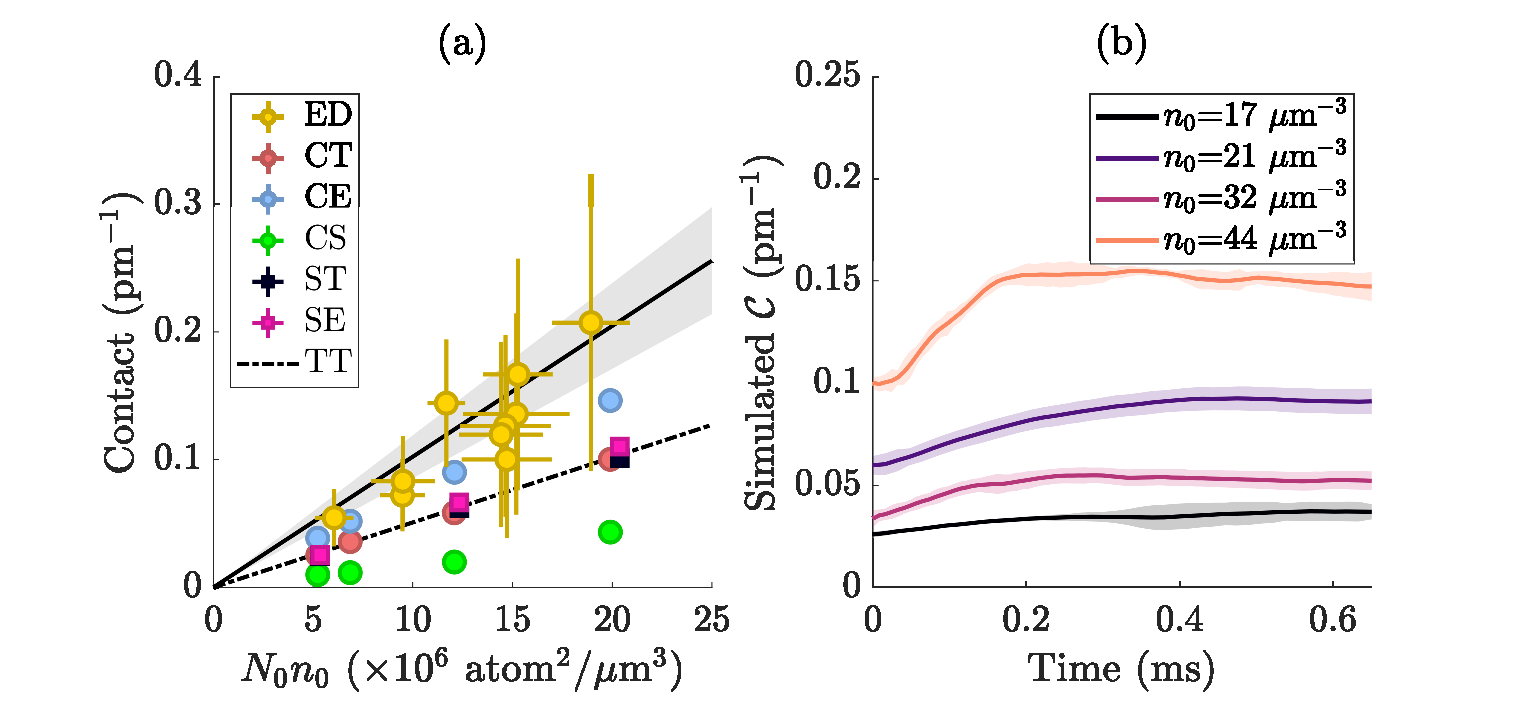
\includegraphics[width=0.5\textwidth]{fig/depletion/main/main/contact_plot_with_theory}
% %         \caption{Comparison of simulations and experiments.
% 	(a) The contact from empirical data (ED) exceeds the prediction by the Tan theory (TT), with trend (and 1$\sigma$ confidence interval) shown as a solid line (grey area).
% 	The simulated contact of BECs in a cigar-shaped trap (CT) are consistent with (TT) before release but compare well with our measurements after expansion (CE).
% 	A slow relaxation of the tight axes of the cigar trap (CS) show a reduction in the large-momentum tails.
% 	Simulations of a spherical trap (ST) show a modest increase after expansion (SE).
% 	(b) Simulations of condensates released from a cigar-shaped trap show an increase in contact after the trap release, stabilizing after a time on the order of 100$\mu$s.}
% %         \label{fig:theory_fig}
% % \end{figure}

% % \begin{table*}[!t]
% %     \begin{tabular}{c c c c c c c}
% %     \hline\hline
% %     Peak density ($\micron^{-3}$) & $N_\textrm{tot}$ ($\times10^5$) & Thermal fraction & ROI counts & Expected counts & $C_\textrm{est}$ ($\times10^{11} m^{-1}$) &$C_\textrm{est}/\mathcal{C}$  \\ 
% %     \hline 
% %     16.9(1.8) & 3.5(4) & 0.09 & 5.6(0.1) & 2.8(0.6) & 5.4(2) & 1.9(0.8) \\ 
% %     18.7(1.4) & 5.0(4) & 0.17 & 6.8(0.1) & 3.7(0.8) & 7.2(3) & 1.8(0.7) \\ 
% %     19.3(2.1) & 4.9(6) & 0.08 & 8.1(0.2) & 4.3(0.9) & 8.3(4) & 1.8(0.8) \\ 
% %     20.4(1.0) & 5.7(3) & 0.09 & 14.8(0.1) & 5.5(1.2) & 1.4(5) & 2.6(0.9) \\ 
% %     38.6(2.6) & 3.9(3) & 0.14 & 4.9(0.1) & 1.9(0.4) & 1.6(9) & 2.5(1.3) \\ 
% %     38.6(3.4) & 3.7(4) & 0.09 & 3.5(0.04) & 1.9(0.4) & 1.1(7) & 1.7(1.0) \\ 
% %     38.6(3.5) & 3.8(4) & 0.11 & 3.7(0.1) & 2.4(0.5) & 1.0(6) & 1.5(0.9) \\ 
% %     38.7(3.4) & 3.7(4) & 0.09 & 4.1(0.1) & 2.1(0.4) & 1.2(7) & 1.8(1.0) \\ 
% %     39.0(4.1) & 3.8(5) & 0.10 & 4.3(0.1) & 2.2(0.4) & 1.3(8) & 1.9(1.1) \\ 
% %     41.3(2.2) & 4.5(4) & 0.12 & 6.5(0.2) & 2.6(0.5) & 2.0(1) & 2.4(1.3) \\ 
% %     \hline\hline
% %     \end{tabular}
% %     \caption{Summary of results for each data run.
% 	The peak density is determined from measurements of the condensed number (via the total number $N_\textrm{tot}$ and condensate fraction) and trapping frequencies, which in turn is used to predict the contact $\mathcal{C}$.
% 	The number of atoms detected in the region of interest can be used to determine the empricial contact $C$ from the $k^{-4}$-like tail by inverting Eqn.
% 	\ref{eqn:pred_num}}
% %     \label{tab:results}
% % \end{table*}

% % \section{Simulations} 
% % To gain further insight we performed simulations of the BEC expansion from a harmonic trap using the Positive-P method, including a cigar-shaped trap with parameters matched to the experimental conditions, and a spherically symmetric trap with identical peak density $n_0$.
% 	The results of these simulations are consistent with the adiabatic sweep theorem before release from the trap, and agree well with our experimental data, as shown in Fig.
% 	\ref{fig:theory_fig} (a).
% 	Following release from the trap, the simulated tail amplitude increased and stabilized at a factor of 1.46(5) above the predictions of \ref{eqn:TotalHarmonicContact} in a few hundred microseconds, much smaller than the 2ms delay between the trap release and application of the rf and Stern-Gerlach pulses.
% 	We also investigated the effect of adiabatic expansion on the in-trap contact by simulating a slow decrease of the trapping frequencies by a factor of two, and found that the in-trap contact decreased in these instances.
	


% % \section{Discussion} We interpret our results as an indication that dispersal of the mean-field energy of the condensate into kinetic energy of the depleted atoms is the mechanism responsible for the disagreement between predicted and measured contact.
% 	In detail, following the quench of the condensate into the free particle regime, the condensate expands hydrodynamically.
% 	This adiabatic reduction in density reduces the local contact density, whereby some depleted atoms are absorbed back into the condensate.
% 	However, the quasiparticles with large $k$ (in the particle branch of the Bogolubov dispersion) have sufficient velocity to escape the cloud before reabsorption.
% 	The relevant timescale for hydrodynamic expansion is on the order of millseconds, while the supersonic depleted particles leave the condensate in microseconds.
% 	Moreover, an atom inside the BEC experiences a force given by the gradient of the mean-field potential (and consequently the density) $F = 4\pi\hbar^2a \nabla  n(x)/m$.
% 	This increases the number of depleted particles with enough energy to escape reabsorption into the condensate, and endows the depleted particles with a greater velocity, leading to an increase in the weight of the tails in the far-field, and of particular relevance to lighter atoms because the acceleration scales with $1/m^2$.
% 	This picture is supported also by the simulations, in which we observe a decrease in the total number of depleted particles coincident with an increase in the large-k population.
	


% % \section{Conclusion}
% % In conclusion, our findings suggest that the quantum depletion is indeed visible in the far-field momentum distribution, and that the hydrodynamic approximation does not capture sufficient microscopic information to make detailed predictions about the high-momentum behaviour.
% 	The interplay between coherent absorption of Bogolubov excitations and the dispersal of the chemical potential into kinetic energy, to which Helium is particularly sensitive, result in overpopulation of the $k^{-4}$ tails of the momentum distribution.
	

% % \section{Future work}
% % The growing suite of far-field investigations \cite{cayla20,chang16} supplemented by this work invite complementary studies of the quantum depletion and contact in situ with ultracold \mhe.
% 	Measurements of the structure factor via Bragg spectroscopy may greatly benefit from the single-particle detection afforded by metastable Helium, which is compelling in light of complications of radio spectroscopy of Helium (discussed in the supplementary material).
% 	An intriguing goal for future studies in Helium is the resolution of particle pairs with opposite momenta in the depleted fraction.
% 	 Such an observation would be challenging because the correlation peak height decreases with the collection efficiency and is broadened by the expnsion dynamics.
% 	Nonetheless, insight into pairing mechanisms in a cold bosonic gas would bear fruit for wider coherent phenomena in condensed matter.


% %     % Leo 2001: The M pairings (1,1),(1,0),(-1,-1), and (-1,0) the collision is dominated by a $^5\Sigma_g ^+$ potential, hence \emph{inelastic processes can occur only via the weak relativistic spin-dipole interaction}.
% 	The scatteering lengths are then almost identical to $a_5$ but with small imag part.
% 	Ilastic rates for (0,0) and (1,-1) from which ionization can occur, are much larger and dominate the total ionization rate for an unpolarized gas.
	
% %     % Ergo - could use RF spectroscopy by modulating the ion production rate via the (1,-1) channel?
% %     % Vassen: $a_{1,-1} \approx 60a_0, a_{1,1} \approx 140 a_0$.
% 	But the chemical potential for each species is different - does this shift the RF resonance? Or affect the ion production rate?
% %     % -> Ion production rate in terms of scattering lengths, spin pol etc?
% %     % -> Find ion production rate from majorana flips: Majorana flip rate x 
% %     % I wonder if contact measurements could just be extracted from the data that Vassen took in 2016?



% % \section{Appendices}
% % \section{Detection}
% %     We use a Roentdek DLD80 multichannel plate and delay-line detector stack \cite{Manning10} with a quantum efficiency of $\sim8\%$, and space and time resolutions of 100 $\mu$m and 3 $\mu$s, respectively \cite{Henson18}.
% 	After the atoms are released from the trap, they fall 859mm to the detector stack, which registers the arrival times and positions $(t_i,x_i,y_i)$ of each atom, indexed by $i$.
% 	The centre of mass of the cloud arrives after a $\tau = 417$ms time of flight.
% 	The velocity of each atom relative to the centre of mass of the cloud is $(v_x,v_y,v_z) = t_{i}^{-1}(x_i,y_i,g_0(\tau^2-t_{i}^{2}))$, where $g_0$ is the local gravitational acceleration.
% 	The velocity conversion carries a negligible error of a few ppm.
% 	We then centre the counts from each realization and detection sequence (termed a \emph{shot}) and transform the counts from cartesian velocity space to spherical polar coordinates with radius $k$ (in $m^{-1}$), polar angle $\theta$ and elevation angle $\phi$, relative to the centre of the cloud, where the velocity-to-wavevector transformation follows from  $\textbf{p}=m\textbf{v}=\hbar\textbf{k}$.
	

% %     The solid angle in k-space available to detect the depleted tails is limited by the 40mm radius of the circular detection surface.
% 	The field of view of our detector is $|k_{x,y}|\approx5\times 10^6$ m$^{-1}$ in the XY plane, which is only just sufficient to reach past the edge of the thermal region.
% 	We sample data from the segments of the sphere with elevation angle $|\phi|>\pi/3$ rad and $|k|<10^7$ m$^{-1}$, centred on the BEC, which encompasses a total solid angle of $0.22\times 4\pi$ steradians.
% 	The detector's dark count rate of $0.56$ Hz cm$^{-2}$ sets the noise floor and contributes an average of 0.4(2) counts to the region of interest per shot.
% 	The distribution of the number of counts in each shot are shown in Fig.
% 	\ref{fig:num_counts}


% % \begin{figure}[!h]
% %     \centering
% %     \includegraphics[width=0.7\textwidth]{fig/depletion/main/som/counts_per_run}
% %     \caption{Number of counts detected in the region of interest across in the depletion measurement (a), the spin mixing calibration (b), and the dark count calibration (c).
% 	An average of 3.0(5) counts were detected in the ROI in the spin-mixing calibration shot, and the background count rate was 0.4(2) counts per shot.}
% %     \label{fig:num_counts}
% % \end{figure}

% % % \todo{Density plots out to larger $|k|$ to show descent into noise floor? How far could we push it until we hit dark counts?}

% % % \section{Spin mixing}
% % % Also lets us determine thermal fraction - note it isn't determinable from the PAL because of the mean-field broadening (but one could just make fits and subtract the thermal part, yes?).
% 	I think the mean-field expansion is particularly bad for Helium, and wasn't reported much before, because we are 5% the mass of popular species like Rb so much more subject to mean-field acceleration!

% % \section{Trap configuration and calibration}

% %     We prepared our BECs with a standard sequence, achieving condensation via forced evaporative cooling in a harmonic magnetic trap with trap frequencies $\sim(425,425,45)$ Hz and a DC bias stabilized by our auxiliary field compensation coils \cite{Dedman07}.
% 	For the tight trap we increased the coil current after the cooling sequence to obtain trapping frequencies $\sim(902,895,71)$ Hz, using a sigmoid step function which to minimize in-trap oscillations.
% 	The trap remained on for 150ms before switching the trap off with a $1/e$ time of $\approx38\mu$s.
% 	The condensates were allowed to expand for 2ms before we transferred some of the condensate into the magnetically insensitive $m_J=0$ state to prevent distortion by stray magnetic fields.
% 	The rf RF sweep generated by a RIGOL function generator, amplified, and applied to the experiment chamber by a coiled antenna inserted into the BiQUIC coil housing.
% 	The pulse swept from 1.6-2.6MHz over 1ms and was centred on the fine structure resonance between the $m_J$ states and transfers atoms into the $m_J = j$ states with efficiencies $\eta_j$.
% 	The sweep was $10^6$-fold wider than the Doppler broadening of the BEC which ensures uniform transfer at all momenta.
% 	Immediately after the RF sweep, the bias coils are switched off and auxiliary push coils in the vertical (Z) and weak horizontal (X) axis are activated using a fast MOSFET switch to implement a Stern-Gerlach separation of the $m_J = -1,~0,$ and $+1$ pulses

% % \subsection{Determining transfer efficiency}

% %     To calibrate the transfer efficiencies, we applied the Stern-Gerlach field for a shorter time, resolving each cloud on the detector.
% 	While the efficiencies $\eta_J$ cannot be calculated by counting the atoms in each cloud because the detector saturates, we can compare the thermal parts.
% 	We align each cloud along the time axis and compute the pointwise proportion of the atomic flux accounted for by each cloud, as depicted in Fig.
% 	\ref{fig:frac_cal}.
% 	The flux fraction of each cloud is roughly constant in the thermal part, indicating the absence of important saturation effects and a spin transfer that is independent of $k$.
% 	The fraction of the total flux of each pulse is identified with the fraction of the original cloud which has been transferred into the respective spin state.
% 	We find these efficiencies are approximately 74\%, 24\%, and 2\% in all runs for the $m_J=+1$, 0, and -1, respectively.
	 
    
% % \begin{figure}[!h]
% %     \begin{center}
% %         \includegraphics[width=0.7\textwidth]{fig/depletion/main/som/frac_cal_profile}
% %         \caption{Determining the rf transfer efficiency.
% 	The time-of-flight profiles of each pulse are aligned with respect their centre-of-mass (a).
% 	The pointwise fraction ((b), dotted line) is uniform where saturation is not evident (solid lines).
% 	Detector saturation is apparent in the peaks of the $m_J=+1$ and $m_J=0$ pulses, but not in the $m_J=-1$ pulse.}
% %         \label{fig:frac_cal}
% %     \end{center}
% %     \end{figure}


% % \subsection{Determination of thermal fraction}
% %     While the $m_J=0$ and $m_J=1$ clouds clearly saturate the detector, the small fraction ($\sim2\%$) in the atoms to the $m_J=-1$ state  does not.
% 	We fit the density outside the condensate with a Gaussian distribution plus constant background and obtain an estimate of the thermal atom number.
% 	Subtracting the number of thermal atoms from the total number in the $m_J=-1$ cloud, minus background counts, yields a estimate of the thermal and condensed fraction, as illustrated in Fig.
% 	\ref{fig:thermal_frac}.

% %     \begin{figure}[!h]
% %     \begin{center}
% %         \includegraphics[width=0.7\textwidth]{fig/depletion/main/som/m1_frac_anal}
% %         \caption{Comparison of thermal fits in the unsaturated $m_J=-1$ pulse including 138 shots.
% 	The weak (X) and strong horizontal (Y) trapping axes are shown in (a) and (b), respectively.
% 	Both projections display a bimodal peak, with the condensate (dotted lines) and thermal parts (thick solid lines) easily distinguished.
% 	Fitting a Gaussian profile (thin solid line) to the velocity distribution of the thermal part yields the thermal number and temperature.
% 	Subtracting the fit leaves the condensate profile (c) which can be yields the condensed number.}
% %         \label{fig:thermal_frac}
% %     \end{center}
% %     \end{figure}



% % \subsection{Analysis of spin transfer measurements}

% %     In early tests of our measurement sequence we noticed a contamination of the signal by spurious counts from the $m_J=+1$ cloud.
% 	We calibrate for this contamination by running the depletion measurement without the RF transfer.
% 	While the cause of the cross-contamination is unclear, we observe that the count density outside the region of interest is similar in both the shots with the RF pulse and those without.
% 	We infer that the remnant counts may be atoms transferred into the $m_J=0$ state by a side effect of the finite switching time of the magnetic fields.
	

% %     % \begin{figure}[!h]
% %     % \begin{center}
% %     %   \includegraphics[width=\textwidth]{fig/depletion/main/som/profile_overlay}
% %     %   \caption{Comparison of average time-of-flight profiles over a single data run for the quantum depletion measurement shots (blue, 871 shots), transfer efficiency calibration (black, 112 shots), detector dark counts (red, 871 shots), and spurious counts (dot-dash, 895 shots).
% 	The time window bounded by $|k|\leq 10\mu$m is indicated with dotted lines.
% 	Shaded area is the standard error over the entire run.}
% %     %   \label{fig:tof_profile}
% %     % \end{center}
% %     % \end{figure}




% % % Note that the temps disagree between axes, but within axes between clouds they are consistent(....ish).
% 	This means we can use the profile ratio method, which is also consistent with comparing the thermal number from the fits.
% % % Perhaps comment on the thermal-subtracted part; the TF profile should have a sharp cutoff, but the smooth edges are suggestive evidence of this roll-off


% % \subsection{Peak density calibration}

% %     The peak density of the condensate can be written as $n_0 = \mu/g$, where $\mu$ is the mean-field energy in the Thomas-Fermi approximation and $g=4\pi\hbar^2a_{1,1}/m$ is the effective interaction strength, in terms of the atomic mass $m$ and $a=7.512$ nm is the s-wave scattering length between pairs of atoms in the $m_J=1$ state \cite{Moal06}.
% 	The expression for the peak density can can be expanded as
% %     \begin{equation}
% %         n_0 = \frac{1}{8 \pi}\left( (15N_0)^2 \left(\frac{m \bar{\omega}}{\sqrt{a_{1,1}} \hbar}\right)   ^{6}\right)^{1/5}
% %         \label{eqn:n0}
% %     \end{equation}
% %     where $\bar{\omega} = \left(\omega_x\cdot\omega_y\cdot\omega_z\right)^{1/3}$ is the geometric trap frequency and $N_0$ is the number of atoms in the condensate.
% 	We simultaneously determine the total atom number $N$ and trap frequency $\bar{\omega}$ in a single shot using a pulsed atom laser and use the thermal fraction to determine the condensed number $N_0$.
	

% %     The pulsed atom laser consists of a series of Fourier-broadened RF pulses centred on the minimum Zeeman splitting in the trap.
% 	The pulse transfers atoms in the trap to the untrapped $m_J=0$ state with an approximately constant transfer rate across the cloud.
% 	We outcouple approximately 2\% of the atoms per 100$\mu$s pulse for $\sim$200 pulses, which eventually depletes the entire trap.
% 	The atom laser thus prevents the detector from saturating and allows an accurate determination of the atom number, up to a factor of the quantum efficiency.
% 	A typical outcome of this procedure is shown in Fig.
% 	\ref{fig:pal_shot}

% %     \begin{figure}[!h]
% %     \centering
% %         \includegraphics[width=0.7\textwidth]{fig/depletion/main/som/pal_shot}
% %         \caption{A kicked pulsed atom laser with motion sampled at 11ms intervals.
% 	The oscillations in the centre-of-mass position of each pulse are shown along the Y axis over time (a).
% 	The apparent frequency can be determined for each axis (b).
% 	The outcoupling efficiency is fixed throughout the sampling sequence (c), producing a geometric decay of the number of atoms in each pulse.
% 	The straight line on a logarithmic scale shows that detector saturation saturation is negligible and that the BEC population does not affect the transfer rate.}
% %         \label{fig:pal_shot}
% %     \end{figure}
    
% % \subsection{Measuring the trapping frequencies}

% %     To illustrate how we obtain the trapping frequencies, consider an undamped harmonic oscillator in one dimension.
% 	The centre-of-mass momentum $p(t) = A \cos(2\pi f t))$ oscillates at a frequency $f$ Hz, and the centre of mass of a pulse outcoupled at time $t'$ lands on the detector at a position $x'(t+\tau) = p(t')\tau/m$, where $\tau$ is the time of flight of the centre of mass.
% 	Sampling the cloud motion with a sampling period T starting at initial time $t_0$ produces a series of pulses whose centres of mass land at $\{x_n = (A\tau/m) \cos(\omega(t_0+nT))\}$.
% 	The sampling frequency $f_s=1/T$ determines the \emph{Nyquist frequency} $f_N=f_s/2$, which is the maximum frequency that can be reconstructed unambiguously from such a sampling regime.
% 	When $f>f_N$ the signal manifests as a lower-frequency oscillation known as the \emph{alias} of the signal.
% 	The aliased frequency $f_a$ is

% %     \begin{equation}
% %      f_a =
% %       \begin{cases}
% %        \frac{Z_n f_s}{2} - f & \text{if } Z_n \text{ even} \\
% %        f - \frac{(Z_n-1)f_s}{2}       & \text{if } Z_n \text{ odd},
% %       \end{cases}
% %       \label{eqn:Z_N}
% %     \end{equation}
    
% %     where $Z_n = \lceil{f/f_N}\rceil$ is the Nyquist zone number, as described in numerous rf engineering references.
% 	While it is not possible to determine $Z_N$ for a signal with an unknown (not necessarily stationary) $f$ from samples taken at a fixed $f_s$, one can vary $f_s$ and determine both $Z_N$ and $f$ from the gradient $d f_a / d f_s$.
	
% % \begin{figure}[!h]
% %     \centering
% %         \includegraphics[width=0.7\textwidth]{fig/depletion/main/som/sawtooth_plot}
% %         \caption{Aliasing of the trap frequency oscillations under different sampling regimes.
% 	The fitted oscillation frequency is shown in each axis for a range of sampling frequencies.
% 	The sawtooth function is a one-parameter fit which determines the underlying frequency of the centre-of-mass oscillations.}
% %         \label{fig:sawtooth_plot}
% %     \end{figure}    

% %     We induce oscillations of the BEC in all three axes by briefly displacing the trap centre with a perturbation to the trapping field.
% 	The maximum sampling frequency is limited by the temporal width of the BEC pulse landing on the detector to about 100Hz, yielding a Nyquist frequency too low to resolve the un-aliased oscillations.
% 	We fit the apparent oscillation frequency in each axis as a function of sampling frequency as shown in Fig.
% 	\ref{fig:sawtooth_plot}, along with a one-parameter fit of Eqn.
% 	\ref{eqn:Z_N}.
% 	We thys determine that the frequencies $(\omega_x,\omega_y,\omega_z)$ of each of the traps used in the experiment are $2\pi\times(45,425,425)$ and $2\pi\times(72,889,893)$, respectively, which are stable to within 5\% throughout the duration of the data collection and to better than $1\%$ in a given run.


% %     \section{Theory}

% % In the Thomas-Fermi approximation, the energy per particle of $N_0$ condensed bosonic atoms is
% % \begin{equation}
% % \frac{E}{N_0} = \frac{5}{7} \mu = \frac{5}{7} \frac{\hbar \bar{\omega}}{2} \left(\frac{15 N_0 a}{a_\textrm{HO}}\right)^{2/5},
% % \end{equation}
% % in terms of the chemical potential $\mu$, where $a_\textrm{HO} = \sqrt{\hbar/(m \bar{\omega})}$ is the harmonic oscillator length \cite{PethickSmith}.
% 	Via the sweep theorem it follows that
% % \begin{equation}
% % \mathcal{C} = \frac{8\pi}{7} \left(15^{2}(a N_0)^{7} \left(\frac{m \bar{\omega}}{\hbar}\right)^{6}\right)^{1/5}.
% % \label{eqn:TotalHarmonicContact}
% % \end{equation}

% % Which by substitution of Eqn \ref{eqn:n0} leads to the expression
% % \begin{equation}
% % \mathcal{C} = \frac{64\pi^2a_{1,1}^{2}}{7}\frac{n_0N_0}{k^4}.
	
% % \label{eqn:TotalHarmonicContact}
% % \end{equation}

% % The Lee-Huang-Yang (LHY) correction to the condensate energy is negligible in our experiments.
% 	The LHY correction for the chemical potential of a uniform condensate with density yields an estimate of the worst-case contribution
% % $$
% % \frac{\partial E}{\partial a_{1,1}} = \mathcal{C}_0\left(1+\frac{64\sqrt{na_{1,1}^{3}}}{3\sqrt{\pi}}\right),
% % $$
% % Where $\mathcal{C}_0$ is the contact computed neglecting the LHY term, and the second term in brackets is the LHY correction which amounts to at most a correction of order 1\%, using the highest $n_0$ observed in our experiments.
% 	In reality the correction will be smaller as the density is not uniform and is bounded above by $n_0$.

% % \subsection{Radio spectroscopic prospects}
% % The basic principle of rf contact spectroscopy is to apply an rf tone which is detuned from the resonance between two spin states, whereby atoms in the initial spin state are coupled to an untrapped channel, thus enabling a differential measurement of the atom number.
% 	The signal strength scales with the difference of reciprocal scattering lengths $\Gamma\propto(1/a_\textrm{i,i}-1/a_\textrm{i,f})$ between initial-initial and initial-final spin states \cite{braaten10,wild12}, which can be manipulated via Feshbach resonance to obtain a good signal.
% 	For He$*$ (spin 1) however, the scattering lengths $a_{1,1}$ and $a_{1,0}$ are identical \cite{Leo01}, rendering the preferred $m_J=1-m_J=0$ transition unusuable.
% 	On the other hand, $a_{1,-1} = 3/7 a_{1,1}$ \cite{vassen16}, and the singlet transition can be driven without populating the $m_J=0$ state.
% 	In principle this could produce a detectable flux of atoms to perform sensitive in-trap contact measurements, however, collisions in the $^1\Sigma_{g}^{+}$ channel have large Penning ionization rates which lead to significant trap losses \cite{Leo01}.
% 	 The ionization products would be detectable by in-vacuum channel electron multipliers but require theoretical work to disentangle from the spectroscopic signal.
% 	Further, such an experiment could not take advantage of a Feschach resonance to increase signal strength or decrease the ionization rate, but it is not \emph{prima facie} impossible.

% % \section{Theoretical methods}
% % To fill in with details of how the P+ simulations were done by Piotr

% % \section{Old material}


% % \subsection{Detection of ultradilute momentum spectra}
% % \label{ssec:qd-model}

% %     Our experiments start with a condensate of helium atoms in the $m_J = +1$ state of the metastable $2^3 S_1$ manifold in a BiQUIC magnetic trap \cite{Dall2007}.
% 	The strongest signal of the depleted tails could be obtained by releasing the BEC from the trap and examining the tails of the detected flux on the detector.
% 	However, the presence of stray DC and transient fields in the chamber would distort the BEC profile and thus also the depletion, in ways that may not be feasible to characterize.
% 	For instance, it is known that our freefall zone contains what is colloquially known as a 'magnetic aperture', which deflects atoms from their freefall trajectory if their transverse momentum is great enough.
% 	This effect is visible in NONEXISTANT FIGURE, which shows the distortion of a thermal cloud, which would otherwise be isotropic.
% 	Indeed, this feature proved problematic in determining the detected count rate from the depleted fraction, because .
% 	Following the method described by Chang \emph{et al} \cite{Chang16}, substantial distortions to the condensate can be avoided by transferring part of the sample to the $m_J=0$ state, which is insensitive to stray magnetic fields.
	

% %     Since for these experiments a precise knowledge of the total atom number and trap frequency is important, we measure the trapped population and trapping frequency at regular intervals throughout each experimental run, using a procedure that avoids detector saturation to measure the atom number and precise determination of the trap frequency.
% 	We identified a contamination of the depletion signal by stray counts attributable to the $m=+1$ state, and calibrate for this by including shots without the RF transfer step.
% 	We also apply corrections for the detector dark count rate and an increased background rate on the leading edge of the condensate, which is attributed to a steady-state leakage of atoms from the trap, due to Majorana flips, Penning ionization, or other collisional effects driving loss.
	

% %     A magnetic field gradient is switched on 5ms after the state transfer pulse, which ensures the magnetically sensitive $M_J = \pm 1$ states are deflected enough to miss the detector.

% %     Since for these experiments a precise knowledge of the total atom number and trap frequency is important, we developed an experimental procedure to regularly calibrate the trapped population and trapping frequency at regular intervals throughout each experimental run, using a procedure that avoids detector saturation to measure the atom number (see supplementary material).
% 	We varied total atom number between 1 and $5\times 10^5$ atoms per condensate by varying the endpoint of the evaporative cooling ramp.

% %     We use two trap configurations with characteristic frequencies $\sim 2\pi\cdot (312,312,52)$ and $2\pi\cdot 666,666,69)$ Hz, which were calibrated on setup by the pulsed atom laser method described earlier in chapter XXX.
	

% %     As in previous chapters, data acquisition shots are interleaved with calibration measurements to predict the key variables 

% %     The trap is switched off in $\sim 100\mu s$ and the atoms allowed to fall 848mm, where they are detected with a multi-channel plate and delay line detector \cite{Manning2010}.
% 	To avoid distortion of the condensate by stray magnetic fields, we transferred approximately 25 - of the condensate into the magnetically insensitive $M_J=0$ state by applying a chirped sine wave 2ms after trap switch-off, swept from 1.6 to 2.6 MHz in 1ms, while a DC magnetic field remained on to preserve the Zeeman splitting between $M_J = {0,\pm 1}$ states.
% 	A magnetic field gradient is switched on after the state transfer pulse, which ensures the magnetically sensitive $M_J = \pm 1$ states are deflected enough to miss the detector.
	

% %     After release from the trap the atoms expand ballistically into the far-field regime, where their position on the detector corresponds to their momentum at trap release.
% 	Therefore we can reconstruct the far-field momentum distribution $n^*(\textbf{k})$ from our detector data.
% 	The observed momentum profile $n^*(\textbf{k})$ cannot be identified completely with the in-trap momentum distribution $n_0(\textbf{k})$ as repulsive interatomic forces distort the profile immediately after release from the trap.
% 	Structure is visible over five orders of magnitude in density, comprised of the condensed, thermal, and depleted fraction before the signal drops below the dark-count background noise.
% 	There is some saturation evident around the low momentum values due to the high atom flux during BEC impact.
% 	Our analysis does not include this part of the momentum profile, and we find evidence that saturation is only an issue during the peak flux, not in the thermal or depleted fractions.

% % The count density from the falling BECs depend explicitly on the trapped population and on the trapping frequencies, necessitating regular calibration of the peak condensate density.
% 	The correction from the detected $m_J=0$ counts to the full condensate profile also requires a measurement of the transfer efficiency of the RF pulse, and a diagnostic of any other sources of detection events, such as detector dark count rate or remnant atoms from the $mJ=\pm 1$ condensates.
% 	In the remainder of this section, I describe the means by which the relevant parameters are calibrated and how they are combined into a model of the detector flux which includes the Tan contact as a free parameter.
% 	In the next section, I describe the algorithm I designed to transform the atomic detection events into an appropriate format to correspond with the model and determine the Tan contact.

% % \subsubsection{Contributions to the model}
    
    
% % \subsubsection{Depletion}
% %     In an ideal world, the experimental procedure is trivial: Form a BEC in a desired trapping configuration, and then release the trap instantaneously and fit the atomic density profile obtained from the DLD image.
% 	Unfortunately, nature intervenes: Because our condensates are formed in a weak-field-seeking state, they are subject to deflection during freefall by stray DC and transient magnetic fields.
% 	These distortions to the BEC profile may be significant at large momenta, although we did not characterize this.
% 	A second potential issue is detector saturation, whereby the trailing side of the BEC is detected with a lower quantum efficiency because of a depletion of charge carriers in the MCP, artificially attenuating the depletion signal.
% 	Both of these issues are ameliorated by transferring a fraction of the condensate into the magnetically insensitive $m_J=0$ shortly after the trap release.
% 	This is achieved by sweeping an RF pulse from 1.6MHz to 2.6MHz, as in \cite{Chang16}, with a DC bias field held on by the Nuller coils.
% 	This field is close to uniform over the scale of the BEC and its freefall path, so by the time the condensate is split into the three spin states, distortions to the cloud would be minimal.

% %     The detection sequence therefore proceeeds with a standard BEC production sequence (as described in INTRODUCTION), with a modified end sequence, pictures in figure QD-SEQUENCE.
% 	The DC bias field is ramped on over 300ms in an exponential ramp with time constant 40ms.
% 	This ensures that no centre-of-mass oscillations are induced in the BEC because of sudden displacements of the trap centre.
% 	The BEC is held for XXX ms to damp out any residual oscillations and is then released.
% 	After 2ms of freefall, the RF chirp is generated by a RIGOL function generator, amplified, and applied to the experiment chamber by a coiled antenna inserted into the BiQUIC coil housing.
% 	The nuller coils are switched off, and the auxiliary push coils in the vertical (Z) and weak horizontal (X?) axis are activated via fast MOSFET switch.
% 	The pulse timing and duration of the push coils required some finessing to minimize the scatter of atoms from a \emph{magnetic aperture} inside the freefall path, as described in later in this section.
% 	The push coils remove the $m_J=\pm 1$ atoms from the detector, so the detector signal is dominated by the undistorted $m_J=0$ cloud.
% 	The cloud then falls freely under gravity through the vacuum chamber, completing the 848mm fall in 417ms.
	

% %     It is important to align the condensates carefully in order to faithfully extract the large-momentum tails.
% 	With an ideal detector, one could simply take the mean of all detected counts.
% 	Because of detector saturation, however, the mean position is heavily biased toward the leading edge of the BEC, and indeed the median (which is robust to outliers) is biased also (it is less robust to skewness).
% 	A workaround can be found in the threefold reflection symmetry of the condensate: The parabolic profile in each principal axis means that if one can identify the edges of the condensate, the centre of mass is at the midpoint along each axis.
% 	This is the basis of the following centering algorithm: For each axis, the atomic detection events are compiled into a histogram as a discrete approximation to the continuous atomic flux.
% 	The region where atomic flux exceeds the background rate by a factor of X is determined to be the BEC region - the extremal positions (or times) with flux above the threshold determine the edges of the condensate, and the mean of these two values determines the centre.
% 	The stages of this algorithm are depicted in figure CENTERING, along with the variation of the BEC centre over the course of a run.
	 

% %     We are concerned with the momentum-space distribution of counts.
% 	The atomic wavevector is related to the in-trap velocity by $\textbf{p}=\hbar\textbf{k} = m\textbf{v}$.
% 	The tranformation from $\textbf{r}-\textbf{r}_0$, where $\textbf{r}_0$ is the centre-of-mass position, is simply a linear transformation $\textbf{v} = \frac{\textbf{r}-\textbf{r}_0}{t_{tof}}$ in the $x$ and $y$ directions.
% 	For $z$, corrections must be made for gravitational acceleration instead given by solving the ballistic trajectories $v_z=-h/t_{tof}-\frac{1}{2}g*t_{tof}$ where $h$ is the fall distance and $g$ is the acceleration under gravity.
% 	\todo{txy-to-vel vs linear error?}

% %     The centred velocity-space counts are then transformed into spherical polar coordinates.
% 	The algorithm is described here is also used for the spin-mixing and dark count calibrations, where the spherical coordinate system is centred at the mean BEC centre-of-mass position in TXY coordinates.
	
% %     \begin{equation}
% %     	(r_i,\theta_i,\phi_i) = (\sqrt{x_{i}^{2}+y_{i}^{2}+z_{i}^{2}},\tan^{-1}(y_i/x_i),\tan^{-1}(z_i/\sqrt{x_{i}^{2}+y_{i}^{2}})
% %     \end{equation}

% %     The counts for each BEC are then compiled into a spherical histogram
% %     \begin{equation}
% %     	N(R(n),\Theta(l),\Phi(m)) = |\{(r_i,\theta_i,\phi_i:r(n)\geq r_i<r(n+1),\theta(l)\geq \theta_i<\theta(l+1),\phi(m)\geq \phi_i<\phi(m+1)\}
% %     \end{equation}
% %     Where $n,l,m$ are indices of the histogram with edges $r(n)$.
% 	Ergh, get this notation sorted out.
	
% %     The memory demands can get exhaustive - holding large TXY datasets and also lots of large 3D histograms - can reduce the by lots of writing to disk, but the cheater way around this was to compute the mean by adding to the histogram by looping over each shot, and ditto the squared number of counts to find the variance later.
% 	There would also be a biasing effect by including the empty bins which are defined outside the detector area.
% 	These are found by a messy case analysis in \verb|find_final_bin_idx.m| (hyperlink to dox html?).
% 	 These are excluded from subsequent sums over profiles.
% 	The bins are normalized by the spherical volume element
% %     % \begin{equation}
% %     \begin{align}
% %     	V(n,l,m) &= \int_{R(n)}^{R(n+1)} d r \int_{\Theta(l)}^{\Theta(l+1)} d \theta \int_{\Phi(m)}^{\Phi(m+1)} d \phi r^2 \sin(\phi)\\
% %     	&= (\Theta(l+1)-\Theta(l))(Cos(\Phi(n)+\frac{pi}{2})-Cos(\Phi(n+1)+\frac{pi}{2}))(\frac{r(n+1)^3-r(n+1)^3}{3})
% %     \end{align}
% %     % \end{equation}
% %     \todo{CHECK THIS 3.}

    

% % \subsubsection{Flux model}

% %     The pointwise density of atom detection events in momentum space can be described by the expression
% %     \begin{equation} 
% %     n(\textbf{k}) = \sum_{m=-1}^{1} n_m(N,\omega_{x,y,z},T,\textbf{k}) + \delta(\textbf{k}) + \lambda(N,\bar{\omega},\textbf{k})\Theta(-\theta)
% %     \end{equation}
% %     The first terms $n_m$ refer to the detected density of atoms from the $m_J=m$ condensates, which depends on the momentum vector  on the total atom number N, the temperature T , and harmonic trapping frequencies $\omega_{x,y,z}$.
% 	The dark count rate $\delta$ is momentum-dependent due to its non-uniformity on the detector.
% 	While the BEC is held in the magnetic trap, it is subject to loss mechanisms such as Majorana transitions, Penning ionization, or three-body recombination, and so `leaks' at a rate rate $\lambda$, which may also manifest a momentum-dependence because of its spatial non-uniformity on the face of the detector.
% 	 When the trapped gas is released, the leak stops, hence the Heaviside theta function $\Theta(-\theta)$ ensures this term only contributes on the lower side of the falling BEC.
% 	The distortion-free depletion signal is found in the contribution $n_{0}(\textbf{k},N,\omega_{x,y,z},T)$.
% 	The calibration protocol described in this section is designed to extract this by subtracting away the various sources of background counts, and also ensure accurate calibration of the experimental parameters $N$, $T$, and $\omega_{x,y,z}$


% %     \begin{figure}
% %     \includegraphics[width=\textwidth]{fig/depletion/main/partition_QD_files_profile_overlay_st.eps}
% %     \label{fig:qd-tof1}
% %     \end{figure}
% %     \begin{figure}
% %     \includegraphics[width=\textwidth]{fig/depletion/main/partition_QD_files_profile_overlay_hf.eps}
% %     \end{figure}

% % \subsubsection{Peak density}
% %     The peak density of the condensate can be derived from the expression for the chemical potential $\mu = g \rho(0)$: (see \cite{PitaevskiiStringariBook16}, pp.181)
% %     % \begin{equation}
% %     \begin{align}
% %     \rho_0 &= \frac{\mu}{U}\\
% %         &= \frac{\hbar\bar{\omega}}{2}\left(\frac{15N_0a_0}{\bar{a}}\right)^{2/5} / 4\pi\hbar^2a_0/m
% %     \end{align}
% %     % \end{equation}
% %     % NB: The N a_0/a_h0 is discussed in \cite{Dalfovo99} and is what determines the interaction/kinetic energy ratio
% %     % for fun: calculate the total energy of the condensate (sum over kinetic energies) - and for different segments?
% %     % what is the healing length 1/sqrt(8 pi n a) and corresponding k scale
% %     Where $N_0$ is the total condensed number, $\bar{\omega} = \left(\omega_x\cdot\omega_y\cdot\omega_z\right)^{1/3}$ is the geometric trap frequency, $a_0=7.512$ nm is the interatomic scattering length \cite{Moal06}, $m$ is the atomic mass, and $\bar{a} = \sqrt{\frac{\hbar}{m\bar{\omega}}}$ is the harmonic oscillator length .
% 	Thus the peak density of the condensate can be determined by a measurement of the trapping frequencies and the total condensate number.
% 	Fortunately, these parameters can be measured simultaneously with the pulsed atom laser method described in chapter TUNEOUT.
% 	As shown in chapter TUNEOUT, the trap frequency is stable to XXX accuracy.
% 	Therefore, even over runs of several hours, the trap frequency variation contributes only YYY much variation in peak density.
% 	The variation in atom number can be as much as XXX per cent, which corresponds to a YYY per cent variation in peak density.
	

% %     \begin{figure}
% %     \includegraphics[width=\textwidth]{fig/depletion/main/calibrate_QD_shots_01_stats.eps}
% %     \label{fig:qd-n0_by_time}
% %     \caption
% %     \title
% %     \end{figure}


% % \subsubsection{Dark counts}
% %     Even when the Helium source is not active, the MCP-DLD detector stack stil registers detection events.
% 	These may be genuine, spontaneous electron detection events seeded by background gas in the chamber or thermal excitation in the MCP, or indeed by transients in the DLD lines that are sufficient to trigger a digital pulse from the discriminator.
% 	These are referred to as \emph{dark counts}, by analogy to the Poissonian electronic noise in digital camera sensors like CMOS arrays.
% 	Indeed, the detector dark counts are uncorrelated events and so form a Poisson distribution \todo{Clarify \& graph of dark count statistics}.
% 	The correction for detector dark counts is entirely analogous to \emph{darkfielding} in precision photography, where images are taken without a light source to correct for detector noise.
% 	The spatial distribution of dark counts is shown in figure FIGURE, the time profile in figure PROFILES, and the calibration procedure is described in the next section.

    
% %     % average dark count rate of 5.6228 kHz/m$^2$.
% 	The evident structure in the dark count rate is accounted for in 

% %     The dark count rate is assumed to be uniform in time.
% 	It may be altered by high atomic fluxes of the condensate itself, but this is not a concern for the following reasons: One, we observe very similar thermal tails both above and below the condensate, suggesting that, at least, the quantum efficiency and dark count rates are not significantly different.
% 	Two, although there are some temporary hotspots on the detector during the peak BEC flux, these are only observed co-temporally with the falling BEC.
% 	The quantum depletion is detected far beyond the regions where this effect is noticable, and so they are not expected to contaminate the signal.

% %     A second source of background counts is the so-called \emph{trap leakage}, which is a measurable increase in the steady-state count rate while a BEC is held in the trap, which is visible in figure \ref{fig:qd-tof1}.
% 	Unlike the dark counts, the trap leakage has no obvious spatial structure.
% 	Correcting for these counts is therefore a matter of computing an average spurious count rate and then subtracting this from the detected count density, as described in the next section.
% 	Because the trap leakage stops when the trap is released, this correction is applied only to the leading side of the condensate.
    
% %     The best way to deal with it would be to extend the hold for ages, and then get heaps of statistics, but in the end I wound up using the 20-odd ms window of hold before drop in each case.
% 	This still gets to within ??? some margin of error when using all the data I have for a given run.
% 	In reality, the leak rate should depend on the BEC number, as, for instance, Majorana losses would induce an exponential decay of the trapped atom number, and Penning ionization losses scale with the squared density.
% 	There would also be density-dependent collision effects feeding the trap leak rate driven by changing the trapping frequencies, and different trap configurations would change the trap centre position, which could affect the detected density of the trap leakage.
% 	However, the count rates are so low that we do have the sensitivity to these effects, and so take a relatively simplistic treatment of the trap leakage, described in the next section.

% % \subsubsection{Transfer efficiency}

% %     The efficiency $\eta_0$ of the population transfer to the $m_J=0$ state is critical in determining the Tan contact, as the factor $1/\eta_0$ is the correction applied to the final signal in order to estimate the true signal density in the original condensate.
	

% %     The RF chirp transfers atoms into the $m_J = m$ states with efficiencies $\eta_m$.
% 	The chirp was adopted because, as described in \cite{Chang16}, it would minimize the momentum-dependence of the spin transfer pulse.
% 	The transfer efficiency cannot be calculated by counting the detected number in each cloud, as the condensates still saturate, leading to incorrect estimates.
% 	This is illustrated in figure SATCH-FRACTION.

% %     Instead, we can take advantage of the fact that the condensates have identical spatial profiles (to within a good approximation), albeit with different amplitudes, c.f.
% 	hydrodynamic expansion - density-dependent effects v small after 2ms?


% %     The momentum distribution of the thermal fraction of a degenerate Bose gas is known to be isotropic (see \cite{PitaevskiiStringariBook16} pp.
% 	160) and constitutes less than 5\% of the total population throughout this experiment.
% 	The momentum distribution of the thermal fraction takes the form

% %     \begin{equation}
% %         n_T(\textbf{k}) = \frac{1}{\lambda_T m \bar{\omega}}g_{3/2}\left(e^{-\beta (\hbar) k^2/2m}\right),
% %     \end{equation}

% %     which is manifestly invariant under rotations about the centre of momentum.
% 	Therefore, integrating over the $k_x$ and $k_y$ directions resolves the $k_z$-dependence of the momentum distribution.
% 	(You can talk through the physics better than this matey).
% 	After centering the clouds using a thresholding procedure described in the \textbf{Depletion} section, the time-of-flight profile of each cloud is divided pointwise by the sum of all the time-of-flight profiles.
% 	In the regions where the detector is unsaturated, the ratios $n_m(\textbf{k})/n(\textbf{k})$, where $n_m(\textbf{k})$ and $n(\textbf{k})$ are the momentum-space density of the $m_J=m$ clouds and the original BEC, respectively, are estimates of the transfer efficiency $\eta_m$, as shown in figure \href{fig:qd-fraction_calibration}.
% 	This figure also shows that detector saturation is not apparent in the thermal fraction of the trailing side of the BEC, and therefore suggests that saturation would be negligible in the depleted wings in the trailing edge.
% 	Further, the uniformity of the determined ratio across the thermal fraction is evidence that the RF transfer efficiency is independent of the particle momentum.

% %     \begin{figure}
% %     \includegraphics[width=\textwidth]{fig/depletion/main/frac_cal.eps}
% %     \label{fig:qd-fraction_calibration}
% %     \caption
% %     \title
% %     \end{figure}

    

% % \subsubsection{Spin-mixing}

% %     In the depletion detection shots, we have observed a remaining presence of $mJ=1$ atoms.
% 	These are visible in figure PROFILES, as the step-up in flux rate at 0.56s in a) and the peak in detector flux at 0.55s in b).
% 	The cause of which is unclear but is suspected to be due to a collision process with a feature inside the chamber, as illustrated in figure CLOUDSMASH.
% 	Regardless of the cause, we calibrate for this contamination (also called \textit{spin mixing}).
% 	by running the depletion measurement without the RF transfer, instead measuring the time-of-flight profile of the $m_J=1$ cloud.
% 	After subtracting the background rates as appropriate, this provides a suitable calibration image for the spurious counts, which is subtracted from the measurement profiles, weighted by the transfer efficiency $\eta_1$.

% %     The count density of the $mJ=1$ states depends on the trapping frequencies, as shown by the clear difference between their contributions to figure PROFILES a) and b).
% 	This is likely because the trap centre and BEC width shifts with changing trap frequencies, so the push coil sequence would, left unchanged, result in different spray patterns on the detector.
% 	Unfortunately, we cannot rule out the presence of $mJ=-1$ counts on the detector without additional calibration (for example, taking yet another shot with a different RF transfer fraction).
% 	However, as the $m_J=-1$ clouds are determined to have about one tenth of the total atom population, and the $m_J=+1$ counts are suppressed by nearly three orders of magnitude by the push coils, if we assume a similar suppression of the $m_J=-1$ cloud then \todo{Worst-case bias of -1 counts}


    


% % \section{Determination of the Tan constant}\label{ssec:qd-processing}


% % 	The fit to the depletion profile $\tilde{n_0(k)}$ is obtained by taking the weighted sum of the k-space images for the depletion, spin-mixing, and dark count rates:

% % 	\begin{equation}
% % 		\tilde{n}_0(k) \approx \frac{1}{\eta_0}\left(n_0(k) - \eta_1(n_1(k)-\delta(k))-\delta_k-\lambda(k)\right)
% % 	\end{equation}

% % 	To avoid detector hotspots and to ensure we only use angular bins which extend far enough in k-space to capture some depletion, we specify the spherical sample region $\{(r_k,\theta,\phi): 1E6<r_k<3E7,\theta_{range},\phi_{range}\}$.
% 	Averaging over the angular bins commutes with the image summation because they're all linear.
% 	This produces one-dimensional radial profiles, as shown in figure K-PROFILES.
% 	The depletion and the thermal tails are isotropic, but the BEC is not, so the BEC peak is not physically representative.
% 	Or, remove it from the plot so it's just thermal - i.e.
% 	plot from the largest TF momentum.
	
    

% %     As in \cite{Chang16} we find the large-$\textbf{k}$ momentum distribution is isotropic, unlike the in-trap mean-field interactions, and conclude that the extreme momenta are not strongly affected by the mean-field.
% %     A typical condensate profile shown in Fig.
% 	\ref{k_profile}.
% 	Structure is visible over five orders of magnitude in density, comprised of the condensed, thermal, and depleted fraction before the signal drops below the dark-count background noise.
% 	There is some saturation evident around the low momentum values due to the high atom flux during BEC impact, however this part of the histogram is not used for the analysis.

% %     The Tan contact parameter is extracted by a fit to BEC density profile after subtracting the calibrated noise profiles.
% 	The functional form
% % 	$$
% %     n_{fit}(k) = \frac{N_{th}g_{3/2}exp(-k^2 \lambda_{dB} ^2 /4\pi)}{1.202(2\pi/\lambda_{dB})^3} + \frac{C}{(2\pi)^3 k^4} + const,
% %     $$

% %     includes contributions from the thermal fraction and depleted fraction and includes the free parameters $N_{th}$ the number of thermal atoms, $\lambda_{dB} = h/\sqrt{2\pi m k_B T}$ the thermal de Brogliewavelength, $const$ a constant to account for the detector background count rate, and $C$ is the scale of the fitted power law assumed to correspond to the Tan contact parameter.
% 	In the local density approximation, $C \approx C_{LDA} = \int d\textbf{r} [16\pi^2 \rho^2(\textbf{r},t)a^2]$, where $a$ is the scattering length and $\rho$ the atomic density.
% 	The initial guess for the fit constant $C$ is set to Tan constant predicted by the peak density and number calibrations.
% 	The initial temperatures are set manually for each directory.
% 	The thermal and the depleted parts of the profile are fitted individually to better constrain fitting parameters, and then a joint function is fitted to find the best overall parametrization.
	
    
% %     We verified the fitting method by analysing a test data set of known parameters, which was generated by the Metropolis-Hastings algorithm, and find the method recovers the test set parameters within a factor less than our experimental uncertainties.
    
% % \subsection{Verifying the method}
    
% %     Reliably estimating the parameters of a power-law distribution is nontrivial\cite{Clauset09}, and the robustness of the fitting method above has not been exhaustively tested.
% 	The LDA prediction is essentially that the single-particle wavefunctions, hence the single-particle probability distribution over momentum, are affected by many-body effects.
% 	One computes the single-particle probability density by dividing the condensate density by the number of particles (hence the $N_0$ term in the LDA), and then the problem of extracting the contact parameter from the data is an exercise in statistical parameter estimation.
% 	As shown by Clauset et al \cite{Clauset09}, fitting these functions tends to produce incorrect estimates of parameters.
% 	The method outlined in Clauset was proven to asymptotically converge with probability 1 to the correct fit parameters of a power law distribution, but would need to be extended to derive a maximum likelihood estimator for a power law overlaid on a constant background.

% % \section{Discussion}
% % \label{qd-discussion}

% % \subsection{Findings}
    
% %     According to theoretical predictions based on the local density approximation \cite{Chang16}, the contact constant $C_{LDA}$ of the depleted fraction should vary linearly with the peak condensate density $n_0$.
% 	This was found in previous experiments\cite{Chang16}, although their scaling factor greater by a factor of $\sim$6.5.
% 	In Fig.
% 	XX, we plot our measured values of $C$ and $n_0$ , identifying the fit parameter $C$ with the contact constant $C_{LDA}$ .
% 	A linear fit to the contact constant variation finds a gradient approximately 1.7 times more than the theory predicts.

% %     Our findings suggests that the visibility of the quantum depletion in the far-field momentum distribution is indeed a real physical effect.
% 	Our findings are corroborated by theoretical work.
% 	However, the question remains open as to why the observed population of the quantum depletion is greater than predicted by the otherwise successful Bogoliubov theory.
% 	Possible confounding factors:
% %     \begin{itemize}
% %     	\item Intra-cloud scattering
% %     	\item Trap switchoff or early-falltime dynamics,switch-off timescale may be relevant (compare \cite{Chang16} with \cite{Qu16}).
% %     	\item $m_J=-1$ counts
% %     \end{itemize}

% % 	We have assumed that the RF transfer is momentum-independent, but this could be violated by inhomogeneities or transients in the magnetic field.
% 	The RF pulse may increase the Penning ionization rate in the depolarized sample, even though the density is low, which would alter the momentum profile.
% 	While applying the magnetic separation pulse, the condensates may scatter off each other.


    


% % \subsection{Future work}
	
% %     A possible future experimental extension is to outcouple atoms using a broadened Raman transition.
% 	This would have the benefit of moving the outcoupled atoms through the cloud rapidly, minimising the effects of repulsive inter-atomic interactions that normally affect the outcoupled profiles.
% 	This should shed some light on whether interactions during trap switch off are the origin of the momentum tails.
% 	One could test the importance of particle scattering or Penning ionization by delaying the Rabi transfer to the $M_J = 0$ state, but this could increase vulnerability to stray magnetic fields.
% 	There is scope to optimize the RF transfer sequence to achieve much higher transfer efficiency for a stronger signal
    
    

    


% \hypertarget{optical-lattice}{%
% \section{Optical lattice}\label{optical-lattice}}
% \chapter{Towards an optical lattice for quantum simulation}
% \section{Quantum $\cap$ Complexity}\label{sec:lat-introduction}
% \section{Optical lattices}\label{lat-history}
% % \subsection{Helium's promise}\label{lat-helium}
% \section{Lattice construction at ANU}\label{ssec:lat-motivation}
% \section*{Future work}\label{lat-futurework}


\chapter{Towards an optical lattice trap for helium}
    


\section{Motivation}
% keep to 1 page
	A keystone in the endeavour of physical science is the ability to foresee physical properties of substances that do not yet exist.
	The art and science of materials engineering dates back at least as far as early ceramic or metallurgical work.
	As humankind has developed more sophsticated and reliable understanding of the mechanisms underlying physical properties, so too has the design of new materials become guided more by principle and prediction than random combinatorial search.
	In the solid-state domain, where large numbers of constituent particles are correlated by non-negligible interactions, this project is particularly challenging because analytical models may be conceivable but analytically intractable, and the typical recourse to numerical computing is prohibited by the onerous demands on computer memory or runtime or both.
	Parallel to the trend of increasing precision and scale of physical models is the widening perspective of theoretical physics founded on the premise that \emph{information is physical}.
	Long has it been said that the workings of nature conform to mathematical language; the welcome infiltration of computer science into physical science now offers bridges from the physical to the computational.
	The concept of \emph{abstraction} is central in computer science and formalizes the notion of substrate-independence.
	This is what allows the realization of universal computing in the Von Neumann architecture, instantiated in enormous variety from the prototypical Colossus and ENIAC to the Summit supercomputer and Arduino microcontrollers.
	Abstracting the notion of abstraction away from computer science and into physics provides grounds for the growing field of \emph{quantum simulators}: If you care about the physics, you care about the Hamiltonian, not the objects that the summation indices refer to.
	The hope, then, is that one can build systems that are governed by  particular (or, perhaps, arbitrary) equations of motion such that your experimental system can generate useful data to constrain the search for new material design at a more affordable rate than conventional computing, when measured in some combination of time, energy, or some other convenient currency.
	One flourishing branch of this field of inquiry is the use of \emph{optical lattices} to synthesize artificial crystals, scaled up some 10,000 times and many orders of magnitude colder than conventional solids.
	The ultracold atoms in such systems then play the role of electrons bound in the ion lattice of solid systems.
	In some of these devices, the sophstication and subtlety of the experiments surpasses direct simulations of solid-state models and encroaches on the central questions about emergent complexity, fundamental particle physics and the arrow of time.
	For all their dizzying capabilities, optical lattices have to date relied upon only coarse measurements of momentum-space information, precluding access to detailed dynamical information such as particle currents and aspects of quasiparticle formation.
	Ultracold metastable helium thus offers a dramatic extension of the questions one can ask of optical lattice simulators.
	This chapter details the early development and ongoing efforts at the ANU \mhe group towards realizing this potential.


\begin{adjustwidth}{1.5cm}{0cm}
\begin{flushright}
\emph{``It might be noted here, for the benefit of those interested in exact solutions, \\
that there is an alternative formulation of the many-body problem:\\
How many bodies are required before we have a problem? \\
G.
	E.
	Brown points out that this can be answered by a look at history.
	\\
In eighteenth-century Newtonian mechanics, the three-body problem was insoluble.
	\\
With the birth of general relativity and quantum electrodynamics
in 1930,\\ the two- and one-body problems became insoluble.
	
And within modern\\
 quantum field theory, the problem of zero bodies
(vacuum) is insoluble.
	\\
So, if we are out after exact solutions, no bodies at all is already too many!"}\\
 - Richard Mattuck\footnote{R.
	Mattuck, \emph{A Guide to Feynman Diagrams in the Many-Body Problem}, Dover Books on Physics (1992)}
\end{flushright}
\end{adjustwidth}

\section{The many-body problem}
\subsubsection*{There's always a bigger Hilbert space}

	it from bit

	The prospect of simulating one quantum system by another goes back at least as far as Feynman \cite{feynman82}, who noted in the 80s that the rapid growth of the Hilbert space with the number of objects $N$ presented a serious obstacle to computational physics.
	More concretely, given two quantum systems $A$ and $B$ with $d_A$ and $d_B$ degrees of freedom each, the natural way to represent the composite of the two systems is the tensor product $\mathcal{H}_C$ of their respective Hilbert spaces $\mathcal{H}_A$ and $\mathcal{H}_B$, whose basis can be written as
	\begin{equation}
		\{\ket{e_C}\} = \{\ket{e_A e_B}\} = \{\ket{a_A}\otimes\ket{e_C}\},
	\end{equation}
	where the dimension of the composite system $d_C = |\{\ket{e}\}| = d_A d_B$; a simple illustration of the resource challenge is that a system of $N$ two-level systems thus has a total dimension $2^N$.
	A pure state can be represented as a vector with $2^N-1$ coefficients (the asymptotically trivial reduction by 1 owing to the normalization of the wavefunction), but a general mixed state must be encoded in a density matrix while tracking $2^{2N-1}-1$  coefficients\footnote{While the density matrix has $2^N\times2^N$ entries, the normalization condition and symmetry properties reduce this slightly, but this is no general recipe for ameliorating the many-body problem.}.
	The Hamiltonian, if similarly stored as a full matrix, has comparable memory requirements.
	If the complex coefficients are to be represented by pairs of floating-point number with single precision (for 8 bytes per coefficient), the memory of a consumer-grade laptop is exhausted by the state vector of 16 two-level systems; the density matrix and hamiltoniane exceed available memory for even smaller systems.
	

	Fortunately it is not always necessary to store the full state vector, density matrix, or Hamiltonian in memory.
	For the latter, a sparse representation suffices as most systems of interest exhibit local coupling only, and so most coupling constants are zero.
	However, matrix diagonalization algorithms exploit tradeoffs between memory use and compute depth, which one must confront when dealing with time-dependent problems or parametrized Hamiltonians.
	The memory requirements for the state vector can also be reduced for purposes of simulations by using inventive representations.
	A full review of numerical techniques is far beyond the scope of this thesis, but we will note that exact diagonalization \cite{zhang10} is complemented by an expanding suite of techniques including matrix product states \cite{schollwoeck11} employing the density-matrix renormalization group iterative method \cite{dechiara08}, the Multiscale entanglement renormalization ansatz \cite{}, more general tensor-network representations, quantum Monte Carlo simulations, and emerging techniques using artificial neural network representations of many-body states \cite{}.
	

	Common classes of computational approach; ground-state solving (variational algorithms), time evolution, ...?
	Physical insight -> dimensionality reduction; where these not obvious, neural networks can do well...
	% -> Sometimes many-body systems are tractable because one can reduce the degrees of freedom; eg meanfield, thermodynamics in the extreme case...
	occasionally one is limited by insoluble equations or intractable integrals, but where exact solutions are absent sometimes asymptotically-correct approximations do OK...
	occasionally we are limited by ingenuity, but in general we are compression-limited in dealing with strongly-correlated systems
	% state of the art of QMC - people have done 3D bose hubbard right, and done exceptionally well.
	

	Quantum-native platforms offer a route by which to circumvent some of these issues; clearly Nature has no trouble evolving the state of some $\mathcal{O}(10^23)$ spins in solid materials; if one encodes the physics of interest \emph{directly} into another quantum system, then the space (memory) requirements of simulating quantum systems is obviated.
	This does present another challenge, which is the means of instantiating the state and the means of implementing state evolution.
	Among a wide class of specialized algorithms with less obvious physical counterparts, such as prime factoring or graph partitioning, quantum simulation is within the purview of universal quantum computers.
	A fairly direct translation of classical techniques to digital quantum computers is \emph{Trotterization}, whereby one approximates the time evolution of the state vector
	\begin{equation}
		\ket{\psi(t)} = \hat{U}(t)\ket{\psi(0)} = \exp(-i\hat{H}t/\hbar)\ket{\psi(0)}
	\end{equation}
	by breaking the unitary evolution into iterative application of an approximate unitary operator with time step $\Delta t$ as
	\begin{equation}
		U_{k} = \exp(-i\hat{H}k\Delta t/\hbar).
	\end{equation}
	More modern and quantum-native approaches include qubitization....
	Quantum simulation basically quantum-state monte carlo for some approaches...

	As of the time of writing this dissertation, the largest digital quantum computers have around 50 qubits, and are not able to implement fault tolerant quantum computation at a physically meaningful scale.
	While the early results claiming a quantum advantage have made it to press, the public sphere has not been informed of any simulations of physical systems that are definitively beyond the reach of modern or near-term classical computers.
	Important milestones have been reached along the way in trapped ions \cite{} and superconducting cirtuits \cite{}
% various forms of isolated quantum systems...
	such that information doesn't leak in (unless you're building a sensor, you want your state to be independent of what's going on around it, other than your controlled inputs)
% 	Optical Nicely isolated, but (??) roadblocks?
% 		% Garanovich et al, Light propagation and localization in modulated photonic lattices and waveguides, physics reports 518, 2012
% 		% Recent xanadu paper?
% 		% Boson sampling result
% 	Trapped ion  fast and high fidelity but envt decoherence is a challenge:
% 		% Blatt et al, Quantum simulation with trapped ions, nature physics 8, 2012
% 		lanyon, universal digial sim https://science.sciencemag.org/content/334/6052/57
% 	Superconductors fast and high fidelity but envt decoherencfe is a challenge:
% 		% Houck et al, on-chip quantum simulation with superconducting circuits, nature pysics 8, 2012

	An important counterpart to universal digital quantum simulation is \emph{analogue} simulation\footnote{So called as they rely on the prinicple of controlling physical systems analogous to the systems of interest, not because of the use of analog signals as in the digital/analog dichotomy.}.
	The closest analogy in classical computing is the ASIC, or application-specific integrated circuit: analogue simulators are direct and dedicated simulations of a specified family of Hamiltonians for exploration of that system in particular.
	The prominent physical platforms for such simulation are in trapped ions \cite{}, others \cite{}, and optical lattices, which are the focus of this chapter.
	While schemes have been proposed for universal quantum computing with neutral atoms in optical lattices \cite{brennen99,henriet20}, this potential is still some way off \cite{markov00}.
	Meanwhile, analog simulation in optical lattices is flourishing.
	For the second time, we will note that `any attempt to produce a comprehensive review is out of date by the time it is published' and, in the below, survey some pivotal results in order to clarify the specific contributions that metastable helium atoms could make to the suite of capabilities in optical lattices.

% 	% ah yes; QMC and the sign problem...
% 	% 	that gravity paper? Sign problem is topological? But so far only a barrier to 'general' solutions?
% 	% 	\cite{ringel17} %https://advances.sciencemag.org/content/3/9/e1701758, https://advances.sciencemag.org/content/6/33/eabb8341.abstract,		https://journals.aps.org/prresearch/abstract/10.1103/PhysRevResearch.2.032060

% high energy phys models, exotic states of matter; forecast to quantum-active matter with native cellular compute...
	insertion of 'agents' directly into a synthetic physical envt

\subsubsection{Quantum simulation with optical lattices}

	Optical lattices found their use in cold-atom science for spectroscopic, interferometric, and atom-optical applications before they burst onto the scene as quantum simulators.
	However, that rich history is beyond our scope here.
	The first headline-grabbing experiment was the achievement of the Mott insulating state\footnote{A hallmark of the Mott insulator is the suppression of number fluctuations at each lattice site (i.e.
	\emph{number squeezing}), which was first observed a year prior in \cite{orzel01}.
	However, the later result was the first to eliminate number fluctuations in 3D - see \cite{morsch06} for discussion.} in a lattice filled with ultracold bosonic atoms \cite{greiner02}, realizing the proposition by Dieter Jaksch \emph{et al.} from three years prior \cite{jaksch98}.
	 The subsequent few years saw an explosion of foundational research and technical development, summarized in the reviews \cite{morsch06,bloch08}, and the following decade heralded many major advances in quantum simulation \cite{bloch12,gross17}.
	Theoretical foundations of the myriad models realized in lattices, and their context in a more general condensed-matter setting, are discussed in \cite{LewensteinLattices, lewenstein07}.

	The central principle of an optical lattice is the careful deployment of the optical dipole force \cite{grimm00} to `paint' a potential energy landscape with a persistent periodic structure.
	A stable laser is reflected back on itself, creating a standing.
	Atoms in this optical field thus subject to a periodic potential along the axis of propagation of the laser.
	For a red-detuned beam, the potential energy is minimized at the intensity maxima, providing transverse confinement as inherited by the structure of the beam.
	If the lasers are in the TEM(0,0) mode, the Gaussian profile provides an approximately harmonic confinement when the kinetic temperature is small.
	At ultralow temperatures, the site-to-site variation of the potential energy is nearly constant.
	Additional laser beams can break the axial symmetry and induce two- or three-dimensional periodic structures.
	The simplest of these is a square lattice, but more complicated geometries can be realized by different optical arrangements.
	Hexagonal honeycomb \cite{jotzu14} and triangular geometries complete the simple tiling structures in 2D, which is extended by the Kagome lattice and the recently-emerging quasicrystal lattices.
	Disorder can be introduced to intentionally break translational symmetry by superposing the speckle pattern of another laser or by collinear propagation of another laser whose wavelength is close to an irrational multiple of the main lattice.
	

	An ever-expanding suite of additional allow the experimentalist to furnish their lattices with sophisticated control over the dynamics.
	For example, by synthesizing complex coefficients in the coupling constants between neighbouring sites, neutral atoms can be made to mimic the motion of charged particles in electromagnetic fields.
	Such synthetic fields underpin the realization of numerous paradigmatic consended-matter models \cite{aidelsburger13,tai17,endres11,rispoli19,jo09,simon11,miyake13,folling07,jotzu14}.
	Efforts are ongoing to extend the reach of the cold-atom lab to simulations of high-energy phenomena like matter coupled to non-abelian gauge fields \cite{zohar16,schweizer19,tagliacozzo13} and the Schwinger effect of particle-antiparticle pair production.
	Through varying parameters such as the ratio of the tunnelling and interaction energies (the latter often achieved via Feshbach resonances), optical lattices permit direct realization of quantum phase transitions \cite{greiner01,eckardt05,jordens08,jo09,haller10,simon11,baumann10,leonard17,landig16,sachdevQPT,endres12,anquez16,clark16} and topological phase transitions \cite{goldman16,nakagawa14}.
	The former occurs when the ground state of a Hamiltonian of the form $H = H_0 + g H_1$ assumes a different character on either side of some critical value $g_c$.
	The latter is concerned emergence of a nonlocal order parameter capturing the long-range entanglement structure inherent in different topological phases.

	Modern work in lattices also permits direct inquiry into the role of entanglement in many-body systems out of equilibrium \cite{amico08,eisert15}.
	Direct observations of the growth and propagation of entanglement coincident with the onset of thermalization \cite{clos16,kaufman16} from an initially pure state cement principles of quantum information into the foundations of thermodynamics \cite{osborne02,osterloh02,isakov11,jiang12,dalessio16,goold16,srednicki94}.
	Further outlining this connection is the utility of so-called `algorithmic cooling' whereby high-entropy portions of the many-body quantum state are explicitly identified and removed \cite{bakr11,rodriguez-briones17,boyin02}.
	The application of disordered and quasirandom lattices has permitted direct inquiry into wavefunction localization \cite{anderson58,dalessio16,goold16,srednicki94,clos16,kaufman16}, wherein the presence of disorder prevents the system from thermalizing and instead retains local information about its initial state over long timescales.

\subsubsection{Quantum state microscopy}

	A key enabler of the myriad studies described above are the techniques of quantum gas microscopy \cite{bakr09,cheuk15,endres11,haller15,miranda15,parsons15,rispoli19,sherson10,miranda17,preiss15a} including single-site measurements of spin and particle parity (and recently even population up to $N=4$ \cite{preiss15a}).
	These techniques also permit site-resolved state preparation.
	Direct access to microscopic information renders density correlations readily measurable \cite{endres11,rispoli19}, and sophisticated interferometric techniques even resolve the degree of entanglement (via the R\`{e}yni entropy) between sites \cite{brydges19,daley12,mouraalves04,palmer05}.
	One aspect which has otherwise been absent from the cold atom toolbox is \emph{momentum microscopy}, as afforded by metastable helium.
	During the course of my PhD, a helium lattice was constructed, and achieved the Mott insulating state, at the Institut d'Optique in Palaiseau \cite{ClementLattice}.
	As shown by the abundance of research based on site-resolved microscopy, as described above, there is a wealth of study that could be done with access to microscopic momentum information; more than one machine will surely not be enough to cover all the interesting ground.
	Moreover, the existence of independent apparatus will permit independent replication of experiments that might yield highly surprising results.
	The remainder of this chapter deals with the particular prospects, and progress towards, an optical lattice for ultracold metastable helium at the ANU.


		Correlation functions factorize in simple cases; Bethe ansatz when things reduce to 2 body??
		Experiment exploit corrfuns 
			\cite{schweigler17}
			\cite{hodgman17}

			Single atom detection
	\cite{ott16} review - entirely position-space?


\section{Realizing the Bose-Hubbard model}
	\cite{grimm00}% optical dipole traps 
	\cite{miller93}% Far-off-resonance optical trap- ping of atoms,'' Phys.
	Rev.
	A 47, R4567–R4570 (1993).
	\cite{barrett01}% ``All-Optical Formation of an Atomic Bose-Einstein Condensate,'' Phys.
	Rev.
	Lett.
	87, 010 404 (2001).
	\cite{cabrera}%-gutierrez18 calibration by sudden phase shift of trapping beam; similar in spirit to trap freq measurements in earlier chap
	\cite{celi14}% proposes use of quantized internal states as an additional lattice dimension, but we would prefer to opt for spatial dimensions here
	\cite{gadway18}% momentum spae lattice even proposed
	\cite{ghose03}% magneto-optical lattice for studies of quantum chaos
	floquet prob worth mentioning?
		perhaps move these alt models up with discussions of various geometries 
	\cite{hooley04}
		difference in density of states due to presece of harmonic potential, even in the strength->0 limit
	\cite{kastberg95}
		lattices briefly held the record for the lowest kinetic temperature record; early (temporary) confinement?
		lattice potentials were actually used a fair bit (eg depletion paper) well before Mott insulator transition realized, which catapulted them into the forefront of the physics community
	\cite{machholm03}
		band structure and excitations of BEC in optical lattice (early work; what did this do first??);
		bloch solns (as in machholm03) are unstable and give way to soliton trains machholm04
	ditto, two level atom in periodic optical potential
		\cite{wilkens91}
	introduction to maximally localized wannier fns
		\cite{marzari00}
	\cite{pavarini11}
		wannier fns tutorial
	original wannier paper
		\cite{wannier37}
	\cite{peik97}
		Early use of lattice for kapitza-dirac scattering?? bloch oscillations of atoms in optical potentials



	\begin{figure}[h]
	\centering
	\includegraphics[width=\textwidth]{fig/apparatus/dipole_optics}
	\caption{Schematic 1550nm optics used in the upstairs experiment.}
	\label{fig:dipole_optics}
	\end{figure}

\subsection{Wannier functions}


\section{Construction of experimental apparatus}

\begin{adjustwidth}{1cm}{0cm}
\begin{flushright}
\emph{``It is not necessary to succeed in order to persevere.
	As long as there is a margin of hope, however narrow, we have no choice but to base all our actions on that margin"}\\
- Leo Szilard\footnote{\emph{LIFE magazine} volume 51, issue 9, 1961 }\\
\end{flushright}
\end{adjustwidth}

This experiment did not start from scratch: An existing helium beamline and MOT chamber formed the foundation for the rest of the construction.
	After some years of disuse, the optics were dirty and certainly required realignment or replacement.
	The optical distribution hardware was present but not functional.
	This section documents the extensions I built towards the goal of reaching BEC in this machine

\subsection*{Infrastructure upgrade}

\subsubsection{First MOT}
\subsubsection{Vacuum system renovation}
% wiki/December_2018_Bake
% wiki/Mid-December_2018_Bake
\subsubsection*{Absorption imaging}

While the greatest comparative advantage of helium, with respect to other atomic species, is the far-field detectability via the MCP-DLD, the more conventional technique of absorption imaging is of great utility for diagnostics.
	Principally, direct imaging of atoms in traps is possible, and the possibly large field of view means rather hihg-temperature clouds can be detected.
	In our apparatus, the absorption imaging setup was particularly advantageous because we were unable to install the MCP-DLD for some time as we were waiting for parts to be machined.
	Meanwhile, absorption imaging proved to be instrumental.

A simple characterization of absorption imaging is that one `takes a photo of the shadow of the atoms' by illuminating the sample with a collimated laser beam, and then projecting the beam onto an appropriate sensor.
	In our apparatus we used a Bobcat model camera manufactured by Xenics.
	The photosites are InGaAs substrate with a 20 $\mu$m pixel pitch, and a 320x256 pixel sensor array.
	The camera received light from the absorption imaging setup depicted in Fig.
	\ref{fig:abs_img}.
	Detailed discussions of the physical principles of this technique are presented in \cite{MakingProbingUnderstanding,TychkovThesis}.
	Here we present a simple picture.

A laser tuned close to resonance with the atomic sample is coupled via optic fibre to the absorption imaging setup.
	The light passes through a polarizing beam splitter and then a half-wave plate to set the polarization, which is useful when imaging in the presence of a bias field.
	The beam is then magnified by a 4:1 telescope to a $\approx1$ cm waist and directed at the atomic sample through the vacuum windows.
	Light on the exit side of the cloud will have been attenuated by a factor $e^{i\phi}A$.
	 The attenuation factor $A=\exp(-\frac{\tilde{n}\sigma_0}{2}\frac{1}{1+\delta^2})$ depends on the column density integrated along the beam axis $\tilde{n} = \int n(x) dx$, the detuning $\delta=2(\omega-\omega_0)/\Gamma$ of the laser from resonane as measured in half-linewidths, and the absorption cross-section which is $3\lambda^2/2\pi$ in the two-level approximation.
	The phase $\phi$ also depends on the atomic density and detuning from resonance, and is in principle useful for techniques like phase contrast imaging, but is not presently used in our experiment.
	The light intensity is recorded by the camera in an exposure time of XXXms in our system.
	The resulting `shadow' image is then followed, within a few milliseconds, with a second laser pulse.
	By this point the atoms have scattered many photons and left the laser path.
	The second image is used as a reference to compute the absorption along each column delineated by the edges of the pixels.
	A light-free image can be used as a `darkfield' to reduce the camera's inherent noise profile.
	The pixel-wise absorption is then found by
\begin{equation}
	\frac{I_\textrm{abs}-I_\textrm{dark}}{I_\textrm{ref}-I_\textrm{dark}}:=t^2(x,y),
\end{equation}
which can be processed by appropriate filtering or smoothing to remove image artefacts.
	The 2D absorption profile can be fitted for further quantitative analysis for purposes of thermometry or determining the atomic population.
% http://www.heliumbec.com/wiki/2017/05/09 - first image?
% wiki/2017/05/31  alignment using vertical BOBCAT creating the 'helium comet'

\subsubsection{Second MOT \& Magnetic trap}
% http://www.heliumbec.com/wiki/2017/02/10
% http://www.heliumbec.com/wiki/2017/04/04
% http://www.heliumbec.com/wiki/2017/06/22
% wiki 2017/06/05 some OK image of magnetic trap; may do better
% wiki/Magnetic_trap no imgs but an old lifetime measurement; looks bad, must have had high pressure
\subsubsection{Dipole trap}
% more detail about these.
	Some examples of absorption imaging results.
% http://www.heliumbec.com/wiki/2017/05/19
	% The saturation intensity of the transition is 0.16 mW/cm$^2$.
	Our imaging power is well below this.
% We observe a weird problem that when the RF evaporator is set to the initial 500ms of 34MHz constant radiation, the frequency to the vertical dipole AOM shifts, causing the beam to move far enough that it no longer hits the fibre.
	Further investigation show that this effect is present between 34-38MHz, but seems to disappear for 33MHz and below as well as 40MHz.
	Oddly though, for the higher initial frequencies when the ramp is swept through the trouble region we see no deviation (although it might be too quick to observe).
	Anyway, for now we just set the initial frequency at 33MHz and move on, and will investigate further some other day.
% LOL
% http://www.heliumbec.com/wiki/2017/07/03 first crack sighting

% http://www.heliumbec.com/wiki/2017/07/04 beam profiling
% http://www.heliumbec.com/wiki/2017/08/14 pesky ion signals..
% http://www.heliumbec.com/wiki/2017/08/16 better traces
% evidence against dipole nature; various 'maxima', short steps led to large variation, diminishing peak shape over consecutive runs despite stable alignment and power etc - eventually found unexpectedly high N2 and CO2, perhaps some organic compound 'ablating' from the laser heat http://www.heliumbec.com/wiki/2017/10/20
% http://www.heliumbec.com/wiki/2017/10/26 first sighting of dipole - abandoned idea of optimizing on ion signal and just took a ton of images while stepping through focus lens posn
% http://www.heliumbec.com/wiki/2017/10/27 img simultaneous with resonant exposure, nice narrow beam, shows diff posn to dipole -> diff refractive index
% http://www.heliumbec.com/wiki/2017/11/20 vert alignment?
% http://www.heliumbec.com/wiki/2017/11/28 vert resonance
% http://www.heliumbec.com/wiki/2017/11/22 horz resonant beam with properly alignd img beam (straight channel)
% http://www.heliumbec.com/wiki/2017/11/24 img of double dipole
% http://www.heliumbec.com/wiki/2017/12/01 nice single dipole? pics
\subsection{Subsequent progress}
\section{Future work}
\subsection*{Construction}

Well, dipole, maybe better automation, certainly better envt controls...
	
\subsection*{Scientific aims}

\section*{Workspace}


		
	Often used in conjunction with eg.
	feshbach resonance 
	have their own noise sources
		\cite{pichler10}% nonequlibrium dynamcics of bosonic atoms in optical lattices: Decoherence of many-body states dues to spontaneous emissions
	Complex potentials with additional optical fields, creating synthetic gauge fields
		\cite{aidelsburger11,aidelsburger13,miyake13}


* Cut my teeth on AO alignment and eventually building
a MOT with an old-school security camera * Assembling new vacuum system
Construction Bakeouts - logs? Ti Sub and NEG improvements * LVIS * MOT 2
* Absorption Imaging * Dipole alignment * Misadventures and eventual
fluke - thanks to Patrick
Vacuum chamber

Optics build inc dipole So when I started, we actually didn't have a
working MOT.
	THere were the optis but they were dirty and eyah.
	So they
didn't have light either.
	Had to build a few AO arms - everything except
the collimator and zeeman slower I think, and the ZS was set up
according to the old paper about that lab, right? THe `optimized' one.
Altough one could certainly design a chirped system to increase yield,
but then I wonder what the density/number limits for a MOT are.
	How much
could we actually obtain, given that we then have to push through the
feed hold into another chamber? SO yeah.
	Two MOTs.
	Anythign exciting to
write about? Maybe not - just ballpark the capture velocities maybe.
	The
dipole diagram and control woudl be worth describing.
	The theory of
dipole trapping would belong here as it's not really relevant? Oh, no,
I'll have to put it in the alignment chapter - well it realyl sits in
the polz part of the tuneout chapter.
	So that'll cover that I guess.
Look over the simulations of the dipole potential.
	Maybe some
simulations of evaporative cooling in the dipole.
	Open source 'em of
course.
	Would be a fun way to try some auto-optimization algorithms for
path optimization.
	Another way to burn some time, I guess, there are a
lot of things in here that are becoming big to-do items! Bu Sequence up
to evap \& dipole Imaging system Diagram, some example images and
calculation of number Small simulations \#\# Progress meanwhile\\
New coils, solder catastrophe, new plates \#\# Issues/What next
Stability: Vibration, temp, vacuum Optics: Power, profile Automatic
optimization Broad goals Fermions Quasirandom lattices Are these
actually resources or what? Next generation laser tech?

Condensed matter models/phenomena; 
	\cite{aidelsburger13}% Realization of the hofstatder hamiltonian with ultracold atoms in optical lattices, phys rev lett 111, 2013
	\cite{tai17}% microscopy of the harper-hofstadter model
	\cite{endres11}% Endres et al, observation of correlated particle-hole pairs and string order in low-dimensional Mott insulatros, science 334, 2011
	\cite{rispoli19}% quantum critical behaviour at the MBL transition
	\cite{jo09}%, itinerant ferromagnetism in a fermi gas of ultracold atoms
	\cite{simon11}%, quantum simulation of antiferromagnetic spin chains in an optical lattice
	\cite{miyake13}% - Hofstader-Harper hamiltonian, realizes a topological insulator that breaks time reversal symmetry, ie a quantum hall insulator -> spintronics
	\cite{folling07}% evidence of microscopic effects 2nd order tunnelling
Bose-Hubbard model
	\cite{ramakumar07}%		numerical study of thermodynamics; exactly diagonalized up to 3D (!) up to 1000 atoms in 1000 sites (!!!) in 1D, 540 sites and 3840 bosons in 2D, and 2500 bosons in 50^3 3D lattice.		how??? supercomputer or smart numerics?
	\cite{freericks94}% phase diagram 
	\cite{hopjan20}% MBL in 1D		numerical paper
	\cite{jaksch05}% 'cold atom hubbard toolbox'		predates gauge field, gas microscopes, dipoles...
	\cite{larcher11}% momentum-space localization in incommensurate lattices (aubry-andre model)
	\cite{rispoli19}% disordered BHM
Phase transitions; classical, quantum, topological, dynamical
		\cite{greiner01}% uantum phase transition from a superfluid to a mott insulator in a gas of ultracold atoms, nature 415
		\cite{eckardt05} transition can also be induced by periodic driving
		\cite{jordens08}% a Mott insulator of fermionic atoms in an optical lattice
		\cite{jo09}%, itinerant ferromagnetims in a fermi gas of ultracold atoms;	emergence of ferromagnetic scale in a gas, not a lattice, with repulsive interactions
		\cite{haller10}% pinning quantum phase transition for a Luttinger liquid of strongly interacting bosons
		\cite{simon11}% quantum simulation of antiferromagnetic spin chains in an optical lattice
		\cite{baumann10}%  Dicke quantum phase transition with a superfluid gas in an optical cavity;Open system, light-matter interactions
		\cite{leonard17}% supersolid formation in a quantu mgas breaking a continuous translational symmetry, nature 543
		\cite{landig16}% quantum phases from competing short- and long-rante interactions in an optical lattice, nature 532
		\cite{sachdevQPT}%, Quantum phase transitions, cambridge univ press
		\cite{endres12}% Higgs mode in SF/MI transition
		\cite{anquez16}% quantum kibble-zurek mechanism in a spin-1 bose-einstein condensate
		\cite{clark16}%, universal space-time scaling symmetry in the dynamics of bosons across a quantum phase transition
		\cite{goldman16}% review of topologial matter in optical lattices
		\cite{nakagawa14}% - non-equilibrium, topological phase transition...
	
		% L D Landau 1937, on the theory of phase transitions, Zh Eskp Teor Fiz 7
Out-of-equilibrium physics
		\cite{eisert15}% review quantum many-body systems out of equilibrium, nature physics 11, 2015
	HEP/particle/novel physical synthesis
		\cite{keilmann11}% proposal for creation of anyons in 1D?
		lattice gauge theories
			proposal
				\cite{zohar16}%
			experiments
				\cite{schweizer19}%, gorg19
		in the pursuit of non-abeliean gauge theories to study quark confinement etc
			\cite{tagliacozzo13}% - optical lattice of rydberg atoms
molecules in lattices
		\cite{yan13} dipolar spin-exchange in lattice confined polar molecules
		\cite{yang19} molecular feshbach resonances
		\cite{yan20} ultracold dipolar molecules with microwave-dressed resonant interaction; enhances interaction above s-wave scattering limit for controlled interactions and immediately applicable in lattices
		\cite{balakrishnan16} review of cold chemistry 
		\cite{yelin06, micheli06} %proposals for QC in dipolar molecules in lattices
foundations
	Thermalization/emergence of thermodynamics
		\cite{anderson58}% anderson localization in random lattices 
		\cite{dalessio16}%, from quantum chaos and eigenstate thermalization to statistical mechancis and thermodynamics, advances in physics 65, 2016
		\cite{goold16}% role of quantum information in thermodynamics
		\cite{srednicki94}% chaos and quantum thermalization, phys rev E 50, 1994
		\cite{clos16}% time-resolved observation of thermalization in an isolatd quantum system, - uses trapped ions
		\cite{kaufman16}%, quantum thermalization through entanglement in isolated many-body systems, science 353, 2016
		Coerent superposition and statistical distributions RSP
			Differentiate between them by the presence of off-diagonal terms in the density matrix - accessible by interferometry (put things in superposition) or changes of basis, right? and captured formally by purity, related to VNE 
	Role of entanglement in the emergence of entropy; many-body information (VNE); ETH/MBL
		\cite{kaufman16}%, quantum thermalization through entanglement in isolated many-body systems, science 353, 2016
		\cite{nandkishore15}% review: many-body localization and thermalization in quantum statistical mechanics, annaual review of condensed matter physics 6
			VNE and the quantum breaking of additive entropy
		\cite{chiu18}%	'direct' measurements of entropy
Jaynes; how much info in a quantum state? landauer; that thesis; 
Entanglement in many-body structure
	\cite{amico08} review 
	Entanglement is a thing!%,	Aspect et al 1982 experimental test of bell's inequalities using time-varying analysers,	Aspect et al 1981 experimental tests of realistic local theories via bell's theorem,	Giustina et al, 2015 significant loophole-free test of bell's theorem with entangled photons,	Hensen et al 2015, loophole-free bell inequailty violation using electron spins separated by 1.3km, nature 562,	Shalm et al, 2015 strong loophole-free test of local realism, phys rev lett 115
	Realism vs locality in many-body systems?
		\cite{osborne02}% entanglement in a simple quantum phase transition, phys rev A 66, 2002
		\cite{osterloh02}%  scaling of entangement cose to a quantum phase transition ??
			shows scaling behaviour in analog to correlation functions at classical phase transitions
		\cite{amico08} entanglement in many-body systems, rev mod phys 80, 2008
	local order parameters not obviously applicable to (eg) quantum hall states RSP 
		\cite{jiang12}%, identifiying topological order by entanglement entropy, nature physics 8
	or spin liquids , but non-local entanglement works.
	
		\cite{isakov11}% topological entanglement entropu of a bose-hubbard spin liquid
			numerical paper on kagome lattice
		\cite{jiang12}%
			numerical study on kagome lattice
	While repeatability of ions and qubits means one can exhaustively computer the density matrix , 
		\cite{neill16}% ergodic dynamics and thermalization in an isolated quantum system
		% Haffner et al, scalable multiparticle entanglement of trapped ions, nature 438
	no known state tomography for lattices of itinerant particles, 
	and instead interferometry techniques are employted, usually by realizing identical copies in parallel
		\cite{brydges19}%  probing reyni entanglement entropy via randomized measurements, science 364
		\cite{daley12}% theoretical proposal: measuring entanglement growth in quench dynamics of bosons in an optical lattice
			using parallel copies and like-site parity measurements to determine reyni entropy
		\cite{mouraalves04}% multipartite entanglement detection in bosons, phys rev lett 93
		\cite{palmer05}% detection and characterization of multipartite entanglement in optical lattices
	Collision of quantum information and condensed matter and computing...
		\cite{bakr11}%	Realization of algorithmic cooling in lattices 
		\cite{rodriguez-briones17}% and exploting interactions for deeper cooling
		\cite{boyin02}% first implementation using NMR spins


gas microscopes; 
	\cite{bakr09}  quantum gas microscope for detecing single atoms in a hubbard-regime optical lattice
	\cite{cheuk15}  quantum-gas microscope for fermionic atoms
	\cite{endres11} observation of correlated particle-hole pairs and string order in low-dimensional Mott insulatros, science 334, 2011
	\cite{haller15}  single atom imaging of fermions in a quantum gas microscope, nature physics 11
	\cite{miranda15} site resolved imaging of ytterbium atoms in a two-dimensional optical lattice phys rev A
	\cite{parsons15} site-resolved imaging of fermionic 6Li in an optical lattice phys rev lett 114
	\cite{rispoli19} quantum critical behaviour at the MBL transition
	\cite{sherson10} single-atom resolved fluorescence imaging of an atomic Mott insulator
	\cite{miranda17} achieve imaging without the laser-cooling required to keep atoms pinned during fluorescence; extends possibility to other species
	\cite{preiss15a} - QGM of bosonic 87Rb, but with two planes resolvable, enabling number measurements beyond parity -> greater dyn range in density correlations
facilitating quantum-state engineering
	\cite{chiu18}%
	\cite{kozlowski17}% proposal for unconventional state engineering via weak measurements
	\cite{preiss15a}% - actually a quantum walk demonstration; somewhere there's a paper showing you can do UQC with walks on strange graphs...
correlation funs
	\cite{endres11}%, observation of correlated particle-hole pairs and string order in low-dimensional Mott insulatros, science 334, 2011
	\cite{rispoli19}% quantum critical behaviour at the MBL transition

% \chapter{Conclusion}
% % \hypertarget{conclusion}{%
% \section{Conclusion}\label{conclusion}}

\chapter{Conclusion}
\markboth{CONCLUSION}{}

\begin{flushright}
\emph{``Good judgment depends mostly on experience, and\\ experience usually comes from poor judgment"} \\- Anonymous\footnote{The origin of this frequently misattributed aphorism is unknown \url{https://quoteinvestigator.com/2017/02/23/judgment/}}
\end{flushright}

\todo{Actually write a conclusion i.e. summary and outlook for the various themes and the field in general.}

\section{Synthesis}\label{sec:synthesis}
\section{Outlook}\label{sec:outlook}
\section{Afterword}\label{sec:afterword}
\section*{Gratitude}\label{sec:gratitude}
\addcontentsline{toc}{section}{Gratitude}

This thesis describes work that consists of the following scientific
contributions: * Martin was wrong * New lines * Weakest transition *
Test of QED * Partial resolution of QD which didn't answer much and
isn't decisive re: theory * work towards a new regime of condensed
matter simulation

It is instructive to reflect on the efficiency of these machines as generators of quantum matter.
	The mass input is X to produce Y condensed atoms and detect only 10\% of them.
	The COP is complicated by the atom loss along the way but if we consider the change in energy of only the charge of atoms distilled to the BEC, then we find a COP of X.
	The duty cycle of about 30mHz means that even with large BECs the average flux rate is only X.
	These are low, but one would do well to recall that the first steam engines had efficiencies below 1\%, and several engineering breakthroughs later brought them towards several tens of percent, and gasoline engines followed a similar trend.
	In the production of BEC in the new machine, the duty cycle is reduced by a factor of ten and the atom number by a factor of two, an increase in the time-coherence product of a factor of twenty.
	The downscaling of helium condensate machines is a nontrivial challenge, but one is brought to wonder about the prospects of future fast-cycling, compact devices routinely creating and manipulating large quantum states.
	As James Watt could not conceive of the full implications of a developed rail network, we too are surely blind to the world we may be building


Lord Kelvin's famous remark - 'aside from two clouds, physics is done' - his arrogance aside, we are in a different position: Rather than a 'nearly done' job with a few details to work out, we are vividly aware of the sites of our ignorance.
	As Einstein (?) said, a well-formulated question contains its own answer; but we are still some ways from determining whether we are even asking the right questions!

\begin{itemize}
% \tightlist
\item
  future specroscopy - prospects for helium 3
\item
  Lattices - possible directions
\item
  Quantum correlations \& foundations experiments
\end{itemize}


A personal reflection.
	Was lured in to the academy by the promise of
questions like `what is the difference between simplicity and
complexity' - when are things simple? When is something intrinsically
hard to represent, even if it exists effortlessly in its own right? This
drew me to lattice - to build something with the hands that would be so
elusive for theory and computing.
	But yeah - that might have been
possible, but I hadn't the background to make reasonable progress in the
three year timeframe of an Australian PhD.
	Also, frankly, I didn't have
the tuition or support and so was left alone for most of the time,
crushing motivation and without praise and squirreled my time away in a
simulation that was much more to my theoretical tastes.
	But hey.
	I have
to find a nice way to dress this up.
	Most of these words won't make it.
So having got these ones out of the way, the hope is that I can move on
from them and think more deliberately about what it is that I would say
here.

The chronological order of work is reversed.
	I should perhaps detail the
actual sequence of events - and frame them as pragmatic decisions from
which I learned some useful things about scoping projects properly.
There isn't really much that window dressing can add here.
	But that's
okay - rather than telling the entire truth, just tell enough of it.
	But
don't let the complexity frighten you out of doing your best to be
honest, at least in this tiny sliver, the final vestiage of the
self-expression that you'd hoped you'd find the opportunity to explore.
This has been an exercise in shedding the ego, however incomplete that
process may yet remain.

\#\#\#A critical reading of science Technology evidently brings us great
things.
	But let us not lose sight of the implicit `right to know' - that
we still embody the notion of a conquest over nature, of mastery of the
other, the greater, the ultimately incomprehensible.
	Let us not fall
victim to our own arrogances, and recall that in our turbulent times,
our investigations come at cost.
	The nature of reality will, according
to our ultimate foundations, remain.
	But the conditions of society in
which we have the ability to pursue them are not guaranteed.
	One can
never predict the outcomes of discoveries, or what miraculous things may
be born of new technologies, but in the problem of allocating compute
power from human wetware - which still retains a certain je ne sais
quois that has not been replicated by industrial-scale algorithms
running in silico - we should be mindful of the hubris of endless
pursuit of the mastery of nature.
	This remains ingrained in our
mythology - that more advanced technology is always worth the price that
is paid.
	In the limit of free, clean energy and post-scarcity
manufacture whereby human labour is eliminated, this may be true.
	But,
unlike the atoms in this thesis, we do not live in vacuum.


\footnote{mathematical models - could be thought of as the quantitative storytelling part of humanity, the things that make it unique - and so there's something really sublime about the exactness of the correspondence with the world}, written extensively about in things like `the unreasonable effectiveness of mathematics' and this correspondence is still explored in the problems of foundations of QM: what exactly does this mathematics say abotu the nature of the world? Why does it run this way? This deep inquiry will always be part of the human spirit, I think, but yeah.
The frontiers of physics now marry the fundamental concepts of matter, energy, and information, and we now find much value in the comptuational perspective even at the quantum level...

Why is it,
	for example, so difficult to efficiently simulate quantum processes?
	Where is the border between efficient and intractable? The proof of
	genuine quantum advantages in certain processes may be one of the most
	profound statements about the nature of reality of this generation.
	Wherefore the nature of this advantage? Perhaps we will know before the
	century is out - perhaps, if ongoing crises arenot addressed - we will
	never know, and the cosmos may miss its chance to delve most deeply into
	its own self-awareness.... Particularly consider the confluence of embedded AI etc etc...


			On new physics: We are searching for a revolution in the margins.
	A hair's width between complex theory and calculations.
	Let's assume the calculations are perfect and the experimental errors are overly cautious.
	What do we find - another term in the standard model? Very well.
	It's true that the Higgs detection was a spectacular vindication.
	Was it a revolution? Did it change how we think of our place in the world, alter what we thought was possible? Maybe if you are a theoretical particle physicist.
	And so with these results; they may contribute to an advance in physics, defined as a change in our model of the world in a more profound way than better precision in the fundamental constants.
	Forgive my skepticism; the 'new physics' we find in these experiments may extend the standard model, but for the 'pure' scientist, the goal is not to extend SM, but to supercede it.
	Of course, if we knew where the revelations were, we would spend our money very differently, but in some sense *search* is inseparable from re*search*, with apologies to etymologists.


Whereas millenia have passed without significant evolution, each generation living the same lives as the last, we are surrounded/circumscribed/immersed in the pervasive myth of progress.
	The undescoring narrative always invites the conscientious scientist to ask the impossible question; \emph{what} is the future we are building? \emph{For whom} are we building it, and \emph{why}? <- perhaps better placed in the afterword, gels with notion we are not in vacuum
	

Let us put ourselves in Pythagoras' shoes. What was it like to have such a rudimentary understanding of mathematics? To be so far away from the interplay of geometry and algebra that we have now? These proofs must have seemed magic - what are we scratching at in these labs of the modern quantum endeavour? Pythagoras was practically deified for discovering what is now taught to ten year olds. Where are we going? What is going to happen next? What are we becoming?

% Schrodinger quote goes here?

\begin{center}
\emph{``The key to discoveries is to look at those\\
 places where there is still a paradox.\\
It’s like the tip of an iceberg.\\
If there is a point of \\
dissatisfaction, \\
take a closer \\
look at it.'' \\}
 \end{center}
\begin{center}
~E. Arikan
 \end{center}

\newpage
\vfill
\begin{centering}
\emph{``We shall not cease from exploration\\
And the end of all our exploring \\
Will be to arrive where we started \\
And know the place for the first time."\\} 
- T. S.	Eliot
\end{centering}
\vfill
% \backmatter
\printbibliography
% \bibliography{bibliography}
% The following publications resulted from works undertaken during the course of this scholarship. Works (1) and (4) constitute the major works of this dissertation. Works (2) and (3) were undertaken in the same measurement campaign as (1) and are discussed at length in the dissertations of their leading authors. Works (5) though (7) are not otherwise included in this dissertation.

% Takes: Title, authors, Journal, Year
\begin{enumerate}
\item{Frequency measurements of transitions from the $2\triplet P_2$ state to the $5 \singlet D_1$, $5\triplet S_1$, and $5\triplet D$ states in ultracold helium, J. A. Ross, K. F. Thomas, B. M. Henson, S. S. Hodgman, A. Truscott, K. G. H. Baldwin, {Physical Review A} (2020) }
\item{Direct measurement of the forbidden $2\triplet S_1 – 3\triplet S_1$ atomic transition in helium,  K. F. Thomas, J. A. Ross, B. M. Henson, S. S. Hodgman, A. G. Truscott, {Physical Review Letters} (2020)}
\item{Testing quantum electrodynamics by measuring a \mhe tune-out wavelength, B. M. Henson, J. A. Ross, K. F. Thomas, C. N. Kuhn, D. K. Shin, S. S. Hodgman, Li-Yan Tang, G. W. F. Drake, A. Truscott, K. G. H. Baldwin, {In preparation}}
\item{Tan's contact and quantum depletion of a condensate expanding from a harmonic trap, J. A. Ross, D. K. Shin, B. M. Henson, S. S. Hodgman, A. G. Truscott, {In preparation}}
\item{Entanglement-based 3D magnetic gradiometry with an ultracold atomic scattering halo, D. K. Shin, J. A. Ross, B. M. Henson, S. S. Hodgman, A. G. Truscott, New Journal of Physics (2020)}
\item{Approaching the adiabatic timescale with machine learning, B. M. Henson, D. K. Shin, K. F. Thomas, J. A. Ross, M. R. Hush, S. S. Hodgman, A. G. Truscott, {Proceedings of the National Academy of Science} (2018)}
\item{Widely tunable, narrow linewidth external-cavity gain chip laser for spectroscopy between 1.0-1.1 $\micron$, D. K. Shin, B. M. Henson, R. I.  Khakimov, J. A. Ross, C. J.  Dedman, S. S.  Hodgman, K. G. H.  Baldwin, A. G.  Truscott, {Optics Express} (2016)}
\end{enumerate}


% In Preparation:
% Trap frequency metrology with Bose-Einstein condensates, B. M. Henson, J. A. Ross, D. K. Shin, K. F. Thomas, S. S Hodgman, A. G. Truscott












% \appendix
\end{document}